\documentclass{article}
\usepackage[latin1]{inputenc}
\DeclareMathAlphabet{\mathrm}{OT1}{cmss}{m}{n}
%try typewrite font instead of roman (mathrm) for clarity
% I guess this must be defined at each math statement since defining it above as mathtt does not work

%\usepackage{amsmath}
%\usepackage{amsfonts}
%\usepackage{amssymb}

%Fix up for poorly hyphenated words.
\hyphenation{meas-ured Micro-wave}

\usepackage[dvips]{geometry}
\usepackage{hyperref}

\usepackage[pstricks,squaren,cdot]{SIunits}	% used for SI units and other symbols like mu

\geometry{
	verbose,
	noheadfoot,
	paperwidth=24in,
	paperheight=36in,
	top=0.0in,
	bottom=0.0in,
	left=0.0in,
	right=0.0in
}

%	textwidth=24in,
%	height=36in

\newfont{\titlefont}{cmssbx10 at 50pt}    %Title Font
%\newfont{\titlefont}{cmbx10 at 50pt}    %Old Title Font
%\newfont{\peoplesize}{cmss10 at 4pt}    %People Font

\usepackage{pstricks,pst-poly,pst-3d,pst-node,pst-tree,pst-grad,pst-plot}
% \usepackage{pstricks,pst-poly,pst-3d,pst-node,pst-tree,pst-grad,pst-char,pst-plot}
% \usepackage{pstricks,pstcol,pst-poly,pst-3d,pst-node,pst-tree,pst-grad,pst-char,pst-plot}
\usepackage{color}
\usepackage{calc}
\usepackage{multido}
\usepackage{graphicx} %for the includegraphics function

%Allow polar co-ordinates (radius,angle) with pstricks
\SpecialCoor

%\pagecolor{Black}
\pagestyle{empty}	% suppress page numbering

\definecolor{Black}{rgb}{0.0,0.0,0.0} %Printer uses this layer as CMYK. For testing, alter the values from 0,0,0.
  
%Some backgrounds must be same black as gradient, cannot use CMYK black.
%Try this trick to make an RGB black for the printhouse, use a black that is not quite black.
\definecolor{RGBBlackBegin}{rgb}{0.001,0.001,0.001}
\definecolor{RGBBlackEnd}{rgb}{0.002,0.002,0.002}

\definecolor{IonizingYellow}{rgb}{.88,.88,0}
\definecolor{Itinerant}{rgb}{0.5,1.0,0.5} %Itinerant frequency color


\definecolor{Brown}{rgb}{0.65,0.16,0.16}
\definecolor{DarkBrown}{rgb}{0.463,0.141,0}
\definecolor{BrightGreen}{rgb}{0.5,1,.5}
\definecolor{LineGray}{rgb}{0.6,0.6,0.6}
\definecolor{Gray80}{rgb}{0.8,0.8,0.8}
\definecolor{Gray20}{rgb}{0.2,0.2,0.2}

\definecolor{FColor}{rgb}{0.8,0.8,1.0} %Frequency label colour
\definecolor{WColor}{rgb}{0.8,1.0,0.8} %Wavelength label colour
\definecolor{EColor}{rgb}{1.0,0.8,0.8} %Energy label colour

\definecolor{DarkRange}{rgb}{0.2,0.2,0.2}
\definecolor{LightRange}{rgb}{0.3,0.3,0.3}

\newlength{\VerticalSeparation}  \setlength{\VerticalSeparation}{.15in} %vertical separation of text boxes

\newlength{\EMRPosition}  \setlength{\EMRPosition}{-1.1in} %vertical centerline for arrows
\newlength{\EMRPositionA} \setlength{\EMRPositionA}{\EMRPosition-0.2in}
\newlength{\EMRPositionB} \setlength{\EMRPositionB}{\EMRPosition+0.1in}
\newlength{\EMRPositionC} \setlength{\EMRPositionC}{\EMRPosition-0.4in} %Far left side of box
\newlength{\EMRPositionD} \setlength{\EMRPositionD}{\EMRPosition+0.3in} %vertical centerline for alternative arrows
\newlength{\EMRPositionE} \setlength{\EMRPositionE}{10.1in} %far right side grey backgrounds on chart

\newlength{\AudioPosition}    \setlength{\AudioPosition}{10.4in} % xpos centerline
\newlength{\AudioPositionA}   \setlength{\AudioPositionA}{\AudioPosition-0.1in} %label left side
\newlength{\AudioPositionB}   \setlength{\AudioPositionB}{\AudioPosition+0.1in} %label right side
\newlength{\AudioPositionC}   \setlength{\AudioPositionC}{\AudioPosition-0.2in} %display box left side
\newlength{\AudioPositionD}   \setlength{\AudioPositionD}{\AudioPosition+0.6in} %display box right side
\newlength{\AudioPositionE}   \setlength{\AudioPositionE}{\AudioPosition+0.2in} %right side of piano keys
\newlength{\AudioPositionF}   \setlength{\AudioPositionF}{\AudioPosition-0.5pt} %left side of centerline
\newlength{\AudioPositionG}   \setlength{\AudioPositionG}{\AudioPosition+0.5pt} %right side of centerline


% set normal size text for math fonts
\newcommand{\D}{\displaystyle}

% Erbium-Doped Fiber Amplifier
% \edfa{center Xpos, bottom Ypos}
  \newcommand{\fiberoptics}[2]{
  \rput(#1){
	\psset{fillstyle=solid,fillcolor=yellow,framesep=2pt,linearc=0,linestyle=none}
	%\psframe[fillstyle=solid,fillcolor=yellow](-.175,.05)(.175,.25)
	\psline[fillstyle=none,linestyle=solid,linewidth=1.5pt,linecolor=yellow](-.17,0)(-.17,.2)(.17,.2)(.17,0)
	\rput(0,.15){\psframebox[fillstyle=solid,framesep=1pt]{\textcolor{Black}{#2}}}
  }}


  %draw a tiny submarine{location}{text}
  % The submarine was drawn using xfig then exported as an "Latex picture + epic macros" then the co-ordinates copied into here below
  \newcommand{\submarine}[2]{
  	\rput(#1){\rput(-.27,-.07){
	\psline[unit=.0006in,linecolor=green,fillstyle=solid,fillcolor=WColor,linestyle=solid,linearc=0]{-}(29,190)(240,217)(268,336)
        (403,315)(414,217)(718,201)
        (957,163)(989,244)(1016,250)
        (1016,158)(1027,152)(1027,104)
        (1016,98)(1016,12)(984,17)
        (957,104)(729,50)(528,28)
        (154,28)(40,55)(18,82)
        (12,158)(29,190)}}
	\rput(#1){\textcolor{Black}{#2}}}

  \newcommand{\timestandard}{\psset{linecolor=Black,linewidth=1pt,linearc=0}
	\psframebox[linestyle=none]{%
		\pscircle[linestyle=none,fillstyle=solid,fillcolor=white]{.11}
		\pscircle[fillstyle=none,linestyle=solid]{.1}
		\psline[fillstyle=none,linestyle=solid]{c-c}(.07;150)(0;0)(.05;30)
		\psline[linestyle=solid](.07;0)(.1;0)
		\psline[linestyle=solid](.07;90)(.1;90)
		\psline[linestyle=solid](.07;180)(.1;180)
		\psline[linestyle=solid](.07;270)(.1;270)
		}
	}

  \newcommand{\weatherstation}{
	\psset{linecolor=white,linewidth=1pt,linestyle=solid,fillstyle=solid,fillcolor=white,linearc=0}
	\psframebox[linestyle=none,fillstyle=none]{
		\pscircle(-.03,0.03){.05}
		\pscircle(0.03,0.03){.05}
		\pscircle(-.03,-.03){.05}
		\pscircle(0.03,-.03){.05}
		\psline(-.12,.05)(0.0,.05)
		\psline(-.11,.02)(0.01,.02)
		\psline(-.10,-.01)(0.02,-.01)
		\rput(0,0){\black W}
		}
  }

  \newcommand{\pager}{
	\psset{linecolor=green,linewidth=0.7pt,linestyle=solid,fillstyle=solid,fillcolor=red,linearc=0}
	\psframebox[linestyle=none,fillstyle=none]{
		\psline(0,0)(0,-.1)
		\pscircle(0,0){.05}
		\rput(0,0){\tiny\black P}
	}
  }


  \newcommand{\wirelessmic}{
	\psset{linecolor=Gray20,linewidth=0.7pt,linestyle=solid,fillstyle=solid,fillcolor=DarkBrown,linearc=0}
	\psframebox[linestyle=none,fillstyle=none]{
		\pscurve[linearc=0.04,linewidth=0.5pt,fillstyle=none](-0.015,0.06)(0,0.07)(0,0.09)(0,0.12)
		\psline[linewidth=1.8pt](0,0.1)(0,0.2)
		\pscircle(0,0.2){.03}
	}
  }


  \newcommand{\astrofilter}[2]{
	\rput(#1){\black\bfseries%\tiny
		%\psline[fillstyle=solid,fillcolor=white,linestyle=none](.10;90)(.10;234)(.10;18)(.10;162)(.10;306)(.10;90)
		%\rput(0,0){\pscircle[fillstyle=solid,fillcolor=white,linestyle=none](0,0){.1}}
		%\rput(0,0){#2}
		%\rput(0,0){\psdots[linecolor=white](.15;0)(.15;40)(.15;80)(.15;120)(.15;160)(.15;200)(.15;240)(.15;280)(.15;320)}
		\psline[linecolor=white,linestyle=solid,linewidth=1pt](-.1,-.07)(-.1,.07)
		\psline[linecolor=white,linestyle=solid,linewidth=1pt](.1,-.07)(.1,.07)
		\psframe[fillcolor=white,fillstyle=solid,linestyle=none](-.1,-.05)(.1,.05)
		\rput(0,0){#2}
	}
  }

  \newcommand{\blip}[2]{
	\rput(#1){
		\pscurve[linestyle=solid,linewidth=.8pt,linecolor=black,fillstyle=solid,fillcolor=white](-.1,0)(-.08,.02)(0,.2)(.08,.02)(.1,0)
		\psline[linestyle=solid,linewidth=.8pt,linecolor=white](-.12,0)(.12,0)
		\rput(0,0.09){\textcolor{Black}{#2}}
	}

  }



%%%%%%%%%%%%%%%%%%%%%%%%%%%%%%%%%%%%%%%%%%%%%%%%%%%%%%%%%%%%%%%%%%%%%%%%%%%%%%%%%%%%%
% Notes:
%  - Calibration of the paper size is done with the "\psset{unit=Xin}" setting below
%    where X should be close to 1.000 depending on your printer.
%  - All rows are spaced 0.5" apart.
%  - All columns are determined by dividing the desired width by 12.
%  - The width should be determined by measuring the circumference of the tube that
%    the chart is to be wrapped around.
%    Measure this accurately or use trial and error to line up the sheet once wrapped
%    around cylinder.
%%%%%%%%%%%%%%%%%%%%%%%%%%%%%%%%%%%%%%%%%%%%%%%%%%%%%%%%%%%%%%%%%%%%%%%%%%%%%%%%%%%%%

\begin{document} %===================================================================
\flushleft

%\tiny
%\scriptsize
%\footnotesize
\small
%\normalsize
%\large
%\Large
%\LARGE
%\huge
%\Huge

\sffamily

\psset{unit=1in}% scaling factor for perfect printer to equal 1.000"
%\psset{unit=1.0041841in}% scaling factor for Home Roland Raven printer to equal 1.000"

\begin{pspicture}(-1,-1)(23,35)

  %black background
  \psframe[fillstyle=solid, fillcolor=Black, linestyle=none, linewidth=0pt](-.8,-.8)(22.8,34.8)

  \rput{0}(-.35,-.6){%Sources of EMR
%This is displayed as a column of images and text

%The sun and most stars produce a wide range of frequencies in the spectrum (almost filling this entire chart). Many of the frequencies are filtered by our atmosphere.

% Sources shown as images in a vertical strip
{\white

\psset{%old style (pre 2005-07-28
	fillcolor=black,
	fillstyle=solid,
	cornersize=absolute,
	linearc=4pt,
	linestyle=solid,
	linewidth=2pt,
	linecolor=FColor}

\psset{%new style after 2005-07-28
	cornersize=absolute,
	linearc=4pt,
	linestyle=solid,
	linewidth=2pt,
	linecolor=FColor,
	fillstyle=gradient,
	gradangle=0,
	gradbegin=RGBBlackBegin,
	gradend=RGBBlackEnd,
	gradmidpoint=1.0}


\psline(0,0)(0,35.1)

\rput{0}(0,35.1){\psframebox{\parbox[t]
	{0.5in}{\centering Sources of EMR}}}
\rput{0}(0,0.1){\psframebox{\parbox[t]
	{0.5in}{\centering Sources of EMR}}}

\rput{0}(0,3){\psframebox{\parbox[t]
	{0.5in}{\centering
\includegraphics{sources/brain.eps} Human Brain}}}

\rput{0}(0,5.65){\psframebox{\parbox[t]
	{0.5in}{\centering
\includegraphics{sources/powerline.eps} Power Lines (50,60Hz)}}}

%50Hz - 25KHz
\rput{0}(0,7.9){\psframebox{\parbox[t]
	{0.5in}{\centering
\includegraphics{sources/induction.eps} Induction Heating}}}

\rput{0}(0,17.6){\psframebox{\parbox[t]
	{0.5in}{\centering
\includegraphics{sources/cellphone.eps} Cell phone}}}

% 2.4GHz
\rput{0}(0,18.595){\psframebox{\parbox[t]
	{0.5in}{\centering
\includegraphics{sources/microwave.eps} Microwave oven}}}

\rput{0}(0,20){\psframebox{\parbox[t]
	{0.5in}{\centering
\includegraphics{sources/radar.eps} Radar}}}

\rput{0}(0,27.2){\psframebox{\parbox[t]
	{0.5in}{\centering
\includegraphics{sources/light1.eps} Light bulb}}}

%unneccessary clutter
%\rput{0}(0,27.8){\psframebox{\parbox[t]
%	{0.5in}{\centering
\includegraphics{sources/light2.eps} Flourescent light bulb}}}

\rput{0}(0,25){\psframebox{\parbox[t]
	{0.5in}{\centering
\includegraphics{sources/people.eps} People}}}

\rput{0}(0,13){\psframebox{\parbox[t]
	{0.5in}{\centering
\includegraphics{sources/radio.eps} Radio tower}}}

\rput{0}(0,32){\psframebox{\parbox[t]
	{0.5in}{\centering
\includegraphics{sources/xray.eps} X-Ray machines}}}

\rput{0}(0,34){\psframebox{\parbox[t]
	{0.5in}{\centering
\includegraphics{sources/radiation.eps} Radioactive elements}}}


}
}

  \rput{0}(.4,-.6){% Sizes shown as images in a vertical strip

% from http://www.cellsalive.com/howbig.htm
% hair = 100um
% dust mite = 200um
% ragweed pollen = 20um
% lymphocite = 17um
% red blood cell = 10um
% bakers yeast = 5um
% E. coli bacteria = 3um
% staphylococcus = 800nm
% ebola virus = 1200nm
% rhinovirus = 30nm

% from http://www.brooklyn.cuny.edu/bc/ahp/CellBio/SaS/SandS.html
% bacteria 1um - 5um

% from http://science.howstuffworks.com/virus-human1.htm
% virus = 17 - 300 nm

\psset{%
	fillcolor=white,
	fillstyle=solid,
	cornersize=absolute,
	linearc=4pt,
	fillstyle=solid,
	fillcolor=white,
	linestyle=solid,
	linewidth=2pt,
	linecolor=WColor}

%\rput{90}(0,0){\psframebox(0,3){
\includegraphics{sizes/earth.eps}}}

\psline(0,0)(0,35.1)

%\psframe[fillstyle=crosshatch,hatchangle=45,hatchcolor=WColor,linewidth=1pt,linestyle=solid, hatchwidth=1pt, hatchsep=8pt](-.25,0)(0.25,35.1)

\rput{0}(0,35.1){\psframebox{\parbox[t]
	{0.5in}{\centering Sizes of EMR}}}
\rput{0}(0,0.1){\psframebox{\parbox[t]
	{0.5in}{\centering Sizes of EMR}}}

% 12,756.32 kilometers
\rput{0}(0,5.277){\psframebox{\parbox[t]
	{0.5in}{\centering
\includegraphics{sizes/earth.eps} Earth 12,756 km}}}

% 100m
\rput{0}(0,13.758){
\psframebox{\parbox[t]
	{0.5in}{\centering
\includegraphics{sizes/field.eps} Football Field 100m}}}

% Buildings (Radio)

% 30 ft (12m)
\rput{0}(0,15.287){
\psframebox{\parbox[t]
	{0.5in}{\centering
\includegraphics{sizes/house.eps} House 12m}}}

% 1ft 308mm
\rput{0}(0,17.929){
\psframebox{\parbox[t]
	{0.5in}{\centering
\includegraphics{sizes/football.eps} Football 308mm}}}


%from http://hypertextbook.com/facts/2000/DannyDonohue.shtml  from World Book Encyclopedia. Chicago: World Book
%proton diamater is too small to include on this chart
%0.000000000001 mm
%0.000000001 um
%0.000001 nm
%0.001 pm
%1 fm
%
%
%The electron diameter is 1/1000 times smaller than the proton
% 1 atto meter
%
%Also from Pauling, Linus. College Chemistry. San Francisco: Freeman, 1964: 57, 4-5.
% The radius of the electron has not been determined exactly but it is known to be less than 1 x 10-13 cm


%baseball 76mm

% 6ft 1.8m
\rput{0}(0,16.656){
\psframebox{\parbox[t]
	{0.5in}{\centering
\includegraphics{sizes/people.eps} People 1.8m}}}% Humans (Radio)


% 1.2cm
\rput{0}(0,20.270){
\psframebox{\parbox[t]
	{0.5in}{\centering
\includegraphics{sizes/bee.eps} Honey Bee 1.2cm}}}% Honey Bee (Microwave)

% Pin Head (Infrared)

% dot on page

% Protozoans (Visible)

% 10um Molecules (Ultraviolet)
\rput{0}(0,25.385){
\psframebox{\parbox[t]
	{0.5in}{\centering
\includegraphics{sizes/cell.eps} Single Cell 10\micro \meter}}}

\rput{0}(0,32.897){
\psframebox{\parbox[t]
	{0.5in}{\centering
\includegraphics{sizes/H2O.eps} Water Molecule 0.3\nano \meter}}}



%3um - 800nm
\rput{0}(0,26.582){
\psframebox{\parbox[t]
	{0.5in}{\centering
\includegraphics{sizes/bacteria.eps} Bacteria 3\micro \meter - 800\nano \meter}}}

%protien

%17-300nm
\rput{0}(0,28.374){
\psframebox{\parbox[t]
	{0.5in}{\centering
\includegraphics{sizes/virus.eps} Virus 17-300\nano \meter}}}

% Atoms (Xray)

% Atomic Nuclei  (Gamma Ray)
}

  \rput{0}(2.4,-.7){\small  % Bands of radio waves (encompassing many other bands)
  %
  %y position = xpos_xvalue/9.8 * 0.5" + nearest xpos_yvalue
  %Ex. xpos results for  750e12 937e12   =    (3.72,27.55)(6.62,27.75)   (5.17,27.65)
  %    3.72/9.8 * 0.5 + 27.5 = 27.690
  %\psframe[fillstyle=solid, fillcolor=BoxColor, linecolor=BoxColor](-0.1,27.690)(9.9,27.838)


  % \wrapuparrow{color}{Ypos 2 decimal places}
  \newcommand{\wrapuparrow}[2]{\rput(9.8,#2){\pscurve[linecolor=#1,fillstyle=none,linewidth=1pt,linestyle=solid]{->}(0,0)(0.1,0.05)(0.02,0.12)}}
  \newcommand{\wrapdnarrow}[2]{\rput(0,#2){\pscurve[linecolor=#1,fillstyle=none,linewidth=1pt,linestyle=solid]{->}(0,0)(-0.1,-0.05)(-0.02,-0.12)}}
  \newcommand{\wrapbtarrow}[2]{
  	\rput(9.8,#2){\pscurve[linecolor=#1,fillstyle=none,linewidth=1pt,linestyle=solid]{->}(0,0)(0.1,0.05)(0.02,0.12)}
  	\rput(0,#2){\pscurve[linecolor=#1,fillstyle=none,linewidth=1pt,linestyle=solid]{->}(0,0)(-0.1,-0.05)(-0.02,-0.12)}}


  %define colours used in this file
  \definecolor{HumanAudioColor}{rgb}{0.2,0.2,0.6}

  \psset{fillstyle=solid,linestyle=none}

  % Bottom end of spectrum fade to black
  \psframe[fillstyle=solid, fillcolor=Black, linecolor=Black](\EMRPositionC,-0.1)(2.9,0.4)
  \psframe[fillstyle=gradient,gradangle=90,gradbegin=Black,gradend=Black,gradmidpoint=1.0,linewidth=0pt,linestyle=none](1.9,-0.1)(2.9,0.4)

  % ULF	Ultra Low Frequency  3 - 30Hz  source  http://www.haarp.alaska.edu/haarp/elf.html
  \psframe[fillcolor=LightRange](\EMRPositionC,3.792)(\EMRPositionE,5.453)

  % ELF	Extremely Low Frequency  30 - 3kHz
  \psframe[fillcolor=DarkRange](\EMRPositionC,5.453)(\EMRPositionE,8.776)

  % VLF	Very Low Frequency	100km - 10km	3kHz - 30kHz
  \psframe[fillcolor=LightRange](\EMRPositionC,8.776)(\EMRPositionE,10.436)

  % LF 	Low Frequency		10km - 1km	30kHz - 300kHz
  \psframe[fillcolor=DarkRange](\EMRPositionC,10.436)(\EMRPositionE,12.097)

  % MF 	Medium frequency 	1km - 100m	300-3000 kHz
  \psframe[fillcolor=LightRange](\EMRPositionC,12.097)(\EMRPositionE,13.758)

  % HF 	High frequency 		100m - 10m	3-30 MHz
  \psframe[fillcolor=DarkRange](\EMRPositionC,13.758)(\EMRPositionE,15.419)

  % VHF	Very High Frequency	10m - 1m	30 - 300 MHz
  \psframe[fillcolor=LightRange](\EMRPositionC,15.419)(\EMRPositionE,17.080)

  % UHF	Ultra High Frequency	1m - 10cm	300MHz - 3GHz
  \psframe[fillcolor=DarkRange](\EMRPositionC,17.080)(\EMRPositionE,18.741)

  % SHF Super High Frequency	10cm - 1cm	3GHz - 30GHz
  \psframe[fillcolor=LightRange](\EMRPositionC,18.741)(\EMRPositionE,20.402)

  % EHF Extremely High Frequency 1cm - 1mm	30GHz - 300GHz
  \psframe[fillcolor=DarkRange](\EMRPositionC,20.402)(\EMRPositionE,22.063)

  % Near Ultraviolet (NUV)		400-300nm  750-1000THz
  \psframe[fillcolor=DarkRange](\EMRPositionC,27.707)(\EMRPositionE,27.916)

  % Medium Ultraviolet (MUV)		300-200nm 1000-1500THz
  \psframe[fillcolor=LightRange](\EMRPositionC,27.916)(\EMRPositionE,28.207)

  % Far Ultraviolet (FUV)		200-100nm 1500-3000THz
  \psframe[fillcolor=DarkRange](\EMRPositionC,28.207)(\EMRPositionE,28.705)

  % Extreme Ultraviolet (EUV)	200-10nm  1500THz - 30PHz
  \psframe[fillcolor=LightRange](\EMRPositionC,28.705)(\EMRPositionE,30.368)




%Large Labels defining the major ranges of EMR
{\large\yellow
\psset{linecolor=yellow,linestyle=solid}
\newlength{\LargeLabelPosition}  \setlength{\LargeLabelPosition}{\EMRPosition+0.7in}
\newlength{\LargeLabelRightPosition}  \setlength{\LargeLabelRightPosition}{\EMRPosition+1.2in}

\newlength{\LargeLabelPositionLeft}  \setlength{\LargeLabelPositionLeft}{\LargeLabelPosition-0.2in}
\newlength{\LargeLabelPositionRight}  \setlength{\LargeLabelPositionRight}{\LargeLabelPosition+0.2in}
%\psframe(\LargeLabelPositionLeft,1)(\LargeLabelPositionRight,34.5)

\uput[180]{0}(\LargeLabelPosition,34.14){GAMMA RAYS}
\psline[linecolor=LightRange](\EMRPositionC,33.690)(\LargeLabelRightPosition,33.690)
\psline{<-}(\LargeLabelPosition,33.690)(\LargeLabelPosition,35.5)


\psline{<->}(\LargeLabelPosition,33.690)(\LargeLabelPosition,30.368)
\uput[180]{0}(\LargeLabelPosition,32.03){X-RAYS}

\psline{<->}(\LargeLabelPosition,30.368)(\LargeLabelPosition,27.707)
\uput[180]{90}(\LargeLabelPosition,29.04){ULTRAVIOLET}

%760-400nm (394-749 THz)
\psline[linecolor=LightRange](\EMRPositionC,27.243)(\LargeLabelRightPosition,27.243)
\psline{<->}(\LargeLabelPosition,27.707)(\LargeLabelPosition,27.243)
\uput[180]{0}(\LargeLabelPosition,27.48){VISIBLE}

\psline[linecolor=LightRange](\EMRPositionC,23.724)(\LargeLabelRightPosition,23.724)
\psline{<->}(\LargeLabelPosition,27.243)(\LargeLabelPosition,23.724)
\uput[180]{0}(\LargeLabelPosition,25.48){INFRARED}

%0.3GHz bottom
\psline{<->}(\LargeLabelPosition,23.724)(\LargeLabelPosition,17.080)
\uput[180]{90}(\LargeLabelPosition,20.40){MICROWAVE}

\psline{<->}(\LargeLabelPosition,17.080)(\LargeLabelPosition,9.144)
\uput[180]{90}(\LargeLabelPosition,13.11){RADIO WAVES}

}


\psset{linestyle=solid}% put linestyle back to the way it was


%Change below two lines to this for angled lines
\rput{2.92}{%
\pstilt{87.08}{% angle_for_rput = arctan (0.5"/pspicture_width), pstilt_angle = 90-rput_angle

%change above two lines to this for straight lines
%\rput{0}{%
%{

  % Make grid lines
  \multido{\nYPosition=0.0+0.5,\nYEndPosition=0.3+0.5}{69}{%  change the last number here to identify number of rows high
  	  \psline[linecolor=LineGray]{C-C}(0.000,\nYPosition)(0.000,\nYEndPosition)
  	  \psline[linecolor=LineGray]{C-C}(0.817,\nYPosition)(0.817,\nYEndPosition)
  	  \psline[linecolor=LineGray]{C-C}(1.633,\nYPosition)(1.633,\nYEndPosition)
  	  \psline[linecolor=LineGray]{C-C}(2.450,\nYPosition)(2.450,\nYEndPosition)
  	  \psline[linecolor=LineGray]{C-C}(3.267,\nYPosition)(3.267,\nYEndPosition)
  	  \psline[linecolor=LineGray]{C-C}(4.083,\nYPosition)(4.083,\nYEndPosition)
  	  \psline[linecolor=LineGray]{C-C}(4.900,\nYPosition)(4.900,\nYEndPosition)
  	  \psline[linecolor=LineGray]{C-C}(5.717,\nYPosition)(5.717,\nYEndPosition)
  	  \psline[linecolor=LineGray]{C-C}(6.533,\nYPosition)(6.533,\nYEndPosition)
  	  \psline[linecolor=LineGray]{C-C}(7.350,\nYPosition)(7.350,\nYEndPosition)
  	  \psline[linecolor=LineGray]{C-C}(8.167,\nYPosition)(8.167,\nYEndPosition)
  	  \psline[linecolor=LineGray]{C-C}(8.983,\nYPosition)(8.983,\nYEndPosition)
  	  \psline[linecolor=LineGray]{C-C}(9.800,\nYPosition)(9.800,\nYEndPosition)
       \psline[linecolor=white]{C-C}(0,\nYPosition)(9.8,\nYPosition)%
   }
%  \psline[linecolor=LineGray]{C-C}(9.8,-0.5)(9.8,-0.2)% wraparound on first line only


  \uput{2pt}[270]( 4.9,-0.1){\psframebox[fillstyle=solid,fillcolor=FColor,linecolor=FColor]{\textcolor{Black}{Frequency}}}
  \uput{2pt}[270]( 5.7,-0.1){\psframebox[fillstyle=solid,fillcolor=WColor,linecolor=WColor]{\textcolor{Black}{Wavelength}}}
  \uput{2pt}[270]( 6.5,-0.1){\psframebox[fillstyle=solid,fillcolor=EColor,linecolor=EColor]{\textcolor{Black}{Energy}}}


  \newcounter{StartHeight}	\setcounter{StartHeight}{3}
  \newcounter{EndHeight}	\setcounter{EndHeight}{4}

  %From Doug Welch: Crosshatch style for non-visible colours
  \psset{fillstyle=crosshatch,linewidth=0pt,linestyle=none, hatchwidth=2pt, hatchsep=1.5pt}


  % Brain waves
  % Delta waves 0.1 3Hz
  \definecolor{Fill}{rgb}{1,0.9,0.9}\psset{hatchcolor=Fill}
  \psframe(6.55,1.05)(9.80,1.25)\wrapuparrow{Fill}{1.15}
  \psframe(0.00,1.55)(9.80,1.75)\wrapbtarrow{Fill}{1.65}
  \psframe(0.00,2.05)(9.80,2.25)\wrapbtarrow{Fill}{2.15}
  \psframe(0.00,2.55)(9.80,2.75)\wrapbtarrow{Fill}{2.65}
  \psframe(0.00,3.05)(9.80,3.25)\wrapbtarrow{Fill}{3.15}
  \psframe(0.00,3.55)(5.73,3.75)\wrapdnarrow{Fill}{3.65}
  \rput(6.55,1.15){\psframebox[framearc=0.25,fillstyle=solid, fillcolor=Fill,linecolor=Black,framesep=1pt]{0.1Hz}}
  \rput(4.9,2.65){\psframebox[fillstyle=solid,fillcolor=Fill,framesep=1pt]{ $\delta$ (Delta brain waves)}}
  {\psset{linecolor=yellow,linestyle=solid,linewidth=1pt}
	\psline{<-}(6.55,1.05)(9.80,1.05)
	\psline{-}(0,1.55)(9.80,1.55)
	\psline{-}(0,2.05)(9.80,2.05)
	\psline{-}(0,2.55)(9.80,2.55)
	\psline{-}(0,3.05)(9.80,3.05)
	\psline{->}(0,3.55)(5.73,3.55)
  }

  % Theta 3-8 Hz
  \definecolor{Fill}{rgb}{1,0.8,0.8}\psset{hatchcolor=Fill}
  \psframe(5.73,3.55)(9.8,3.75)\wrapuparrow{Fill}{3.65}
  \psframe(0.00,4.05)(9.8,4.25)\wrapdnarrow{Fill}{4.15}
  \rput(5.73,3.65){\psframebox[framearc=0.25,fillstyle=solid, fillcolor=Fill,linecolor=Black,framesep=1pt]{3Hz}}
  \rput(4.9,4.15){\psframebox[fillstyle=solid,fillcolor=Fill,framesep=1pt]{$\theta$ (Theta brain waves)}}
  \rput(9.8,4.15){\psframebox[framearc=0.25,fillstyle=solid, fillcolor=Fill,linecolor=Black]{8Hz}}
  {\psset{linecolor=yellow,linestyle=solid,linewidth=1pt}
	\psline{<-}(5.73,3.55)(9.8,3.55)
	\psline{->}(0.00,4.05)(9.8,4.05)
  }

  % Alpha 8-12Hz
  \definecolor{Fill}{rgb}{1,0.7,0.7}\psset{hatchcolor=Fill}
  \psframe(0.00,4.55)(5.73,4.75)
  \rput(0,4.65){\psframebox[framearc=0.25,fillstyle=solid, fillcolor=Fill,linecolor=Black,framesep=1pt]{8Hz}}
  \rput(2.87,4.65){\psframebox[fillstyle=solid,fillcolor=Fill,framesep=1pt]{$\alpha$ (Alpha brain waves)}}
  \psline[linecolor=yellow,linestyle=solid,linewidth=1pt]{<->}(0.00,4.55)(5.73,4.55)

  % Low Beta 12-15
  \definecolor{Fill}{rgb}{1,0.6,0.6}\psset{hatchcolor=Fill}
  \psframe(5.73,4.55)(8.89,4.75)
  \rput(5.73,4.65){\psframebox[framearc=0.25,fillstyle=solid, fillcolor=Fill,linecolor=Black,framesep=1pt]{12Hz}}
  \rput(6.82,4.65){\psframebox[fillstyle=solid,fillcolor=Fill,framesep=1pt]{$\beta$ (Low Beta brain waves)}}
  \psline[linecolor=yellow,linestyle=solid,linewidth=1pt]{<->}(5.73,4.55)(8.89,4.55)

  % Mid Beta 15-18
  \definecolor{Fill}{rgb}{1,0.5,0.5}\psset{hatchcolor=Fill}
  \psframe(8.89,4.55)(9.8,4.75)\wrapuparrow{Fill}{4.65}
  \psframe(0.00,5.05)(1.67,5.25)\wrapdnarrow{Fill}{5.15}
  \rput(8.89,4.65){\psframebox[framearc=0.25,fillstyle=solid, fillcolor=Fill,linecolor=Black,framesep=1pt]{15Hz}}
  \rput(0.7,5.15){\psframebox[fillstyle=solid,fillcolor=Fill,framesep=1pt]{$\beta$ (Mid Beta brain waves)}}
  {\psset{linecolor=yellow,linestyle=solid,linewidth=1pt}
	\psline{<-}(8.89,4.55)(9.8,4.55)
	\psline{->}(0.00,5.05)(1.67,5.05)
  }

  % High Beta 18-30Hz
  \definecolor{Fill}{rgb}{1,0.4,0.4}\psset{hatchcolor=Fill}
  \psframe(1.67,5.05)(8.89,5.25)
  \rput(1.67,5.15){\psframebox[framearc=0.25,fillstyle=solid, fillcolor=Fill,linecolor=Black,framesep=1pt]{\textcolor{white}{18Hz}}}
  \rput(5.28,5.15){\psframebox[fillstyle=solid,fillcolor=Fill,framesep=1pt]{$\beta$ (High Beta brain waves)}}
  \psline[linecolor=yellow,linestyle=solid,linewidth=1pt]{<->}(1.67,5.05)(8.89,5.05)

  % Gamma 30Hz
  \definecolor{Fill}{rgb}{1,0.3,0.3}\psset{hatchcolor=Fill}
  \psframe(8.89,5.05)(9.8,5.25)\wrapuparrow{Fill}{5.15}
  \psframe(0.00,5.55)(3.0,5.75)\wrapdnarrow{Fill}{5.65}
  \psframe[fillstyle=gradient,gradangle=90,gradbegin=Fill,gradend=DarkRange,gradmidpoint=1.0,linewidth=0pt,linestyle=none](3.0,5.55)(4.0,5.75)
  \rput(8.89,5.15){\psframebox[framearc=0.25,fillstyle=solid, fillcolor=Fill,linecolor=Black,framesep=1pt]{\textcolor{white}{30Hz}}}
  \rput(1.5,5.65){\psframebox[fillstyle=solid,fillcolor=Fill,framesep=1pt]{$\gamma$ (Gamma brain waves)}}
  {\psset{linecolor=yellow,linestyle=solid,linewidth=1pt}
	\psline{<-}(8.89,5.05)(9.8,5.05)
	\psline{->}(0.00,5.55)(4.0,5.55)
  }

  %The Schumann resonances
  % Schumann resonances


\blip{9.44,4.0}{S}%7.8 Hz
\blip{7.91,4.5}{S}%14 Hz
\blip{3.15,5.0}{S}%20 Hz
\blip{6.86,5.0}{S}%26 Hz
\blip{0.44,5.5}{S}%33 Hz
\blip{2.80,5.5}{S}%39 Hz
\blip{4.82,5.5}{S}%45 Hz


  %Power supply transmission frequencies
  %Power lines

  % 50Hz Power Lines used in Europe
  \psframe[framearc=0, fillstyle=solid, fillcolor=FColor,linewidth=0pt,linestyle=none](5.9,5.5)(6.72,5.8)
  \rput(6.31,5.73){50Hz Power}
  \rput(6.02,5.58){
	\psframebox[linestyle=none,fillstyle=none]{
		\psset{linestyle=solid,linecolor=Black,linewidth=1pt,fillstyle=none}
		\psline[linestyle=solid,linecolor=gray](0.2,0)(.64,0)
		\rput(0.05,0){v=}
		\parabola(0.24,0)(0.27,.07)\parabola(0.30,0)(0.33,-.07)
		\parabola(0.36,0)(0.39,.07)\parabola(0.42,0)(0.45,-.07)
		\parabola(0.48,0)(0.51,.07)\parabola(0.54,0)(0.57,-.07)
	}
  }
  \psframe[framearc=0, fillstyle=crosshatch, fillcolor=FColor,linewidth=0pt,linestyle=none, hatchcolor=FColor,hatchsep=1.5pt,hatchwidth=.2pt](5.9,5.8)(6.72,6.0)
  \psframe[framearc=0, fillstyle=solid, fillcolor=FColor,linewidth=0pt,linestyle=none](5.9,6.0)(6.72,6.3)
  \rput(6.31,6.23){100Hz Lights}
  \rput(6.02,6.08){
	\psframebox[linestyle=none,fillstyle=none]{
		\psset{linestyle=solid,linecolor=Black,linewidth=1pt,fillstyle=none}
		\psline[linestyle=solid,linecolor=gray](0.2,-.07)(.64,-.07)
		\rput(0.05,0){p=}
		\parabola(0.24,0)(.255,.07)\parabola(0.27,0)(.285,-.07)
		\parabola(0.30,0)(.315,.07)\parabola(0.33,0)(.345,-.07)
		\parabola(0.36,0)(.375,.07)\parabola(0.39,0)(.405,-.07)
		\parabola(0.42,0)(.435,.07)\parabola(0.45,0)(.465,-.07)
		\parabola(0.48,0)(.495,.07)\parabola(0.51,0)(.525,-.07)
		\parabola(0.54,0)(.555,.07)\parabola(0.57,0)(.585,-.07)
	}
  }

  %60Hz Power Lines
  \psframe[framearc=0, fillstyle=solid, fillcolor=FColor,linewidth=0pt,linestyle=none](8.48,5.5)(9.3,5.8)
  \rput(8.89,5.73){60Hz Power}
  \rput(8.6,5.58){
	\psframebox[linestyle=none,fillstyle=none]{
		\psset{linestyle=solid,linecolor=Black,linewidth=1pt,fillstyle=none}
		\psline[linestyle=solid,linecolor=gray](0.2,0)(.64,0)
		\rput(0.05,0){v=}
		\parabola(0.24,0)(0.27,.07)\parabola(0.30,0)(0.33,-.07)
		\parabola(0.36,0)(0.39,.07)\parabola(0.42,0)(0.45,-.07)
		\parabola(0.48,0)(0.51,.07)\parabola(0.54,0)(0.57,-.07)
	}
  }
  \psframe[framearc=0, fillstyle=crosshatch, fillcolor=FColor,linewidth=0pt,linestyle=none, hatchcolor=FColor,hatchsep=1.5pt,hatchwidth=.2pt](8.48,5.8)(9.3,6)
  \psframe[framearc=0, fillstyle=solid, fillcolor=FColor,linewidth=0pt,linestyle=none](8.48,6)(9.3,6.3)
  \rput(8.89,6.23){120Hz Lights}
  \rput(8.6,6.08){
	\psframebox[linestyle=none,fillstyle=none]{
	\psset{linestyle=solid,linecolor=Black,linewidth=1pt,fillstyle=none}
	\psline[linestyle=solid,linecolor=gray](0.2,-.07)(.64,-.07)
	\rput(0.05,0){p=}
	\parabola(0.24,0)(.255,.07)\parabola(0.27,0)(.285,-.07)
	\parabola(0.30,0)(.315,.07)\parabola(0.33,0)(.345,-.07)
	\parabola(0.36,0)(.375,.07)\parabola(0.39,0)(.405,-.07)
	\parabola(0.42,0)(.435,.07)\parabola(0.45,0)(.465,-.07)
	\parabola(0.48,0)(.495,.07)\parabola(0.51,0)(.525,-.07)
	\parabola(0.54,0)(.555,.07)\parabola(0.57,0)(.585,-.07)
	}
  }

{\psset{fillstyle=none, linecolor=FColor, linestyle=solid, linewidth=.5pt, linearc=1pt}
\psbezier{->}(5.9,5.6)(4.9,5.6)(4.9,6.65)(2.59,6.65)
\psbezier{->}(8.48,5.6)(7.7,5.6)(7.7,6.65)(5.17,6.65)
} 
% Third harmonics of power lines, suggested by Poul-Henning Kamp
\psframe[framearc=0, fillstyle=solid, fillcolor=FColor,linewidth=0pt,linestyle=none](1.88,6.5)(2.6,6.8)
  \rput(2.24,6.71){150Hz}
  \rput(2.24,6.59){3rd harmonic}
\psframe[framearc=0, fillstyle=solid, fillcolor=FColor,linewidth=0pt,linestyle=none](4.46,6.5)(5.18,6.8)
  \rput(4.82,6.71){180Hz}
  \rput(4.82,6.59){3rd harmonic}


  %Airplane Power
  \psframe[framearc=0, fillstyle=solid, fillcolor=FColor,linewidth=0pt,linestyle=none](5.90,7)(6.72,7.3)
  \rput(6.31,7.23){400Hz}\rput(6.31,7.07){Airplane Power}






  %AM Radio information
{

\psset{linewidth=1pt, linestyle=solid}

  % AM radio 540-1600kHz (two rows)
  %from http://www.dxing.com/tuning.htm
  \definecolor{Fill}{rgb}{0.4,0.68,0.86}
  \psframe[fillstyle=solid, fillcolor=Fill,linewidth=0pt,linestyle=none](0.42,12.55)(9.8,12.75)\wrapuparrow{Fill}{12.65}
  \psframe[fillstyle=solid, fillcolor=Fill,linewidth=0pt,linestyle=none](0.0,13.05)(5.97,13.25)\wrapdnarrow{Fill}{13.15}
  %\rput(0.15,12.65){530kHz}
  %\rput(6.91,13.15){1710kHz}

  % Extended band up to 1610-1710kHz
  \psframe[fillstyle=crosshatch, linewidth=0pt,linestyle=none, hatchwidth=2pt, hatchsep=1.5pt,hatchcolor=Fill](6.06,13.05)(6.83,13.25)

  %\rput(4.9,12.7){AM Radio}
  \rput(4.9,12.75){\psframebox[framesep=2pt,framearc=0.2,fillstyle=solid, fillcolor=Fill,linewidth=0pt,linestyle=none]{AM Radio}}

%draw baselines on each row for scale
\psline{|<*-}(0.42,12.55)(9.80,12.55)
\psline{->|*}(0.00,13.05)(5.97,13.05)

  \rput(0.42,12.65){\psframebox[framesep=1pt,framearc=0,fillstyle=solid, fillcolor=Fill,linewidth=0pt,linestyle=none]{540}}
  \rput(1.91,12.65){600}
  \rput(4.09,12.65){700}
  \rput(5.97,12.65){800}
  \rput(7.64,12.65){900}
  \rput(9.13,12.65){1000}
  \rput(0.68,13.15){1100}
  \rput(1.91,13.15){1200}
  \rput(3.04,13.15){1300}
  \rput(4.09,13.15){1400}
  \rput(5.06,13.15){1500}
  \rput(5.97,13.15){\psframebox[framesep=1pt,framearc=0,fillstyle=solid, fillcolor=Fill,linewidth=0pt,linestyle=none]{1600}}

%I noticed that my AM car radio starts at 530kHz and goes up by 10kHz to 1710kHz
%generated by scale.c with settings of 530e3 1710e3 10e3

%Note: 1600-1710 is the `recently' expanded band


%\psline(0.15,12.55)(0.15,12.57)% 	point=530000.00 	position=19.02 	ypos=19
\psline(0.42,12.55)(0.42,12.57)% 	point=540000.00 	position=19.04 	ypos=19
\psline(0.68,12.55)(0.68,12.57)% 	point=550000.00 	position=19.07 	ypos=19
\psline(0.93,12.55)(0.93,12.57)% 	point=560000.00 	position=19.10 	ypos=19
\psline(1.18,12.55)(1.18,12.57)% 	point=570000.00 	position=19.12 	ypos=19
\psline(1.43,12.55)(1.43,12.57)% 	point=580000.00 	position=19.15 	ypos=19
\psline(1.67,12.55)(1.67,12.57)% 	point=590000.00 	position=19.17 	ypos=19
\psline(1.91,12.55)(1.91,12.60)% 	point=600000.00 	position=19.19 	ypos=19
\psline(2.14,12.55)(2.14,12.57)% 	point=610000.00 	position=19.22 	ypos=19
\psline(2.37,12.55)(2.37,12.57)% 	point=620000.00 	position=19.24 	ypos=19
\psline(2.60,12.55)(2.60,12.57)% 	point=630000.00 	position=19.26 	ypos=19
\psline(2.82,12.55)(2.82,12.57)% 	point=640000.00 	position=19.29 	ypos=19
\psline(3.04,12.55)(3.04,12.57)% 	point=650000.00 	position=19.31 	ypos=19
\psline(3.25,12.55)(3.25,12.57)% 	point=660000.00 	position=19.33 	ypos=19
\psline(3.47,12.55)(3.47,12.57)% 	point=670000.00 	position=19.35 	ypos=19
\psline(3.68,12.55)(3.68,12.57)% 	point=680000.00 	position=19.38 	ypos=19
\psline(3.88,12.55)(3.88,12.57)% 	point=690000.00 	position=19.40 	ypos=19
\psline(4.09,12.55)(4.09,12.60)% 	point=700000.00 	position=19.42 	ypos=19
\psline(4.29,12.55)(4.29,12.57)% 	point=710000.00 	position=19.44 	ypos=19
\psline(4.48,12.55)(4.48,12.57)% 	point=720000.00 	position=19.46 	ypos=19
\psline(4.68,12.55)(4.68,12.57)% 	point=730000.00 	position=19.48 	ypos=19
\psline(4.87,12.55)(4.87,12.57)% 	point=740000.00 	position=19.50 	ypos=19
\psline(5.06,12.55)(5.06,12.57)% 	point=750000.00 	position=19.52 	ypos=19
\psline(5.25,12.55)(5.25,12.57)% 	point=760000.00 	position=19.54 	ypos=19
\psline(5.43,12.55)(5.43,12.57)% 	point=770000.00 	position=19.55 	ypos=19
\psline(5.62,12.55)(5.62,12.57)% 	point=780000.00 	position=19.57 	ypos=19
\psline(5.80,12.55)(5.80,12.57)% 	point=790000.00 	position=19.59 	ypos=19
\psline(5.97,12.55)(5.97,12.60)% 	point=800000.00 	position=19.61 	ypos=19
\psline(6.15,12.55)(6.15,12.57)% 	point=810000.00 	position=19.63 	ypos=19
\psline(6.32,12.55)(6.32,12.57)% 	point=820000.00 	position=19.65 	ypos=19
\psline(6.49,12.55)(6.49,12.57)% 	point=830000.00 	position=19.66 	ypos=19
\psline(6.66,12.55)(6.66,12.57)% 	point=840000.00 	position=19.68 	ypos=19
\psline(6.83,12.55)(6.83,12.57)% 	point=850000.00 	position=19.70 	ypos=19
\psline(7.00,12.55)(7.00,12.57)% 	point=860000.00 	position=19.71 	ypos=19
\psline(7.16,12.55)(7.16,12.57)% 	point=870000.00 	position=19.73 	ypos=19
\psline(7.32,12.55)(7.32,12.57)% 	point=880000.00 	position=19.75 	ypos=19
\psline(7.48,12.55)(7.48,12.57)% 	point=890000.00 	position=19.76 	ypos=19
\psline(7.64,12.55)(7.64,12.60)% 	point=900000.00 	position=19.78 	ypos=19
\psline(7.80,12.55)(7.80,12.57)% 	point=910000.00 	position=19.80 	ypos=19
\psline(7.95,12.55)(7.95,12.57)% 	point=920000.00 	position=19.81 	ypos=19
\psline(8.10,12.55)(8.10,12.57)% 	point=930000.00 	position=19.83 	ypos=19
\psline(8.25,12.55)(8.25,12.57)% 	point=940000.00 	position=19.84 	ypos=19
\psline(8.40,12.55)(8.40,12.57)% 	point=950000.00 	position=19.86 	ypos=19
\psline(8.55,12.55)(8.55,12.57)% 	point=960000.00 	position=19.87 	ypos=19
\psline(8.70,12.55)(8.70,12.57)% 	point=970000.00 	position=19.89 	ypos=19
\psline(8.84,12.55)(8.84,12.57)% 	point=980000.00 	position=19.90 	ypos=19
\psline(8.99,12.55)(8.99,12.57)% 	point=990000.00 	position=19.92 	ypos=19
\psline(9.13,12.55)(9.13,12.60)% 	point=1000000.00 	position=19.93 	ypos=19
\psline(9.27,12.55)(9.27,12.57)% 	point=1010000.00 	position=19.95 	ypos=19
\psline(9.41,12.55)(9.41,12.57)% 	point=1020000.00 	position=19.96 	ypos=19
\psline(9.55,12.55)(9.55,12.57)% 	point=1030000.00 	position=19.97 	ypos=19
\psline(9.68,12.55)(9.68,12.57)% 	point=1040000.00 	position=19.99 	ypos=19
\psline(0.02,13.05)(0.02,13.07)% 	point=1050000.00 	position=20.00 	ypos=20
\psline(0.15,13.05)(0.15,13.07)% 	point=1060000.00 	position=20.02 	ypos=20
\psline(0.29,13.05)(0.29,13.07)% 	point=1070000.00 	position=20.03 	ypos=20
\psline(0.42,13.05)(0.42,13.07)% 	point=1080000.00 	position=20.04 	ypos=20
\psline(0.55,13.05)(0.55,13.07)% 	point=1090000.00 	position=20.06 	ypos=20
\psline(0.68,13.05)(0.68,13.10)% 	point=1100000.00 	position=20.07 	ypos=20
\psline(0.80,13.05)(0.80,13.07)% 	point=1110000.00 	position=20.08 	ypos=20
\psline(0.93,13.05)(0.93,13.07)% 	point=1120000.00 	position=20.10 	ypos=20
\psline(1.06,13.05)(1.06,13.07)% 	point=1130000.00 	position=20.11 	ypos=20
\psline(1.18,13.05)(1.18,13.07)% 	point=1140000.00 	position=20.12 	ypos=20
\psline(1.31,13.05)(1.31,13.07)% 	point=1150000.00 	position=20.13 	ypos=20
\psline(1.43,13.05)(1.43,13.07)% 	point=1160000.00 	position=20.15 	ypos=20
\psline(1.55,13.05)(1.55,13.07)% 	point=1170000.00 	position=20.16 	ypos=20
\psline(1.67,13.05)(1.67,13.07)% 	point=1180000.00 	position=20.17 	ypos=20
\psline(1.79,13.05)(1.79,13.07)% 	point=1190000.00 	position=20.18 	ypos=20
\psline(1.91,13.05)(1.91,13.10)% 	point=1200000.00 	position=20.19 	ypos=20
\psline(2.02,13.05)(2.02,13.07)% 	point=1210000.00 	position=20.21 	ypos=20
\psline(2.14,13.05)(2.14,13.07)% 	point=1220000.00 	position=20.22 	ypos=20
\psline(2.26,13.05)(2.26,13.07)% 	point=1230000.00 	position=20.23 	ypos=20
\psline(2.37,13.05)(2.37,13.07)% 	point=1240000.00 	position=20.24 	ypos=20
\psline(2.48,13.05)(2.48,13.07)% 	point=1250000.00 	position=20.25 	ypos=20
\psline(2.60,13.05)(2.60,13.07)% 	point=1260000.00 	position=20.26 	ypos=20
\psline(2.71,13.05)(2.71,13.07)% 	point=1270000.00 	position=20.28 	ypos=20
\psline(2.82,13.05)(2.82,13.07)% 	point=1280000.00 	position=20.29 	ypos=20
\psline(2.93,13.05)(2.93,13.07)% 	point=1290000.00 	position=20.30 	ypos=20
\psline(3.04,13.05)(3.04,13.10)% 	point=1300000.00 	position=20.31 	ypos=20
\psline(3.15,13.05)(3.15,13.07)% 	point=1310000.00 	position=20.32 	ypos=20
\psline(3.25,13.05)(3.25,13.07)% 	point=1320000.00 	position=20.33 	ypos=20
\psline(3.36,13.05)(3.36,13.07)% 	point=1330000.00 	position=20.34 	ypos=20
\psline(3.47,13.05)(3.47,13.07)% 	point=1340000.00 	position=20.35 	ypos=20
\psline(3.57,13.05)(3.57,13.07)% 	point=1350000.00 	position=20.36 	ypos=20
\psline(3.68,13.05)(3.68,13.07)% 	point=1360000.00 	position=20.38 	ypos=20
\psline(3.78,13.05)(3.78,13.07)% 	point=1370000.00 	position=20.39 	ypos=20
\psline(3.88,13.05)(3.88,13.07)% 	point=1380000.00 	position=20.40 	ypos=20
\psline(3.99,13.05)(3.99,13.07)% 	point=1390000.00 	position=20.41 	ypos=20
\psline(4.09,13.05)(4.09,13.10)% 	point=1400000.00 	position=20.42 	ypos=20
\psline(4.19,13.05)(4.19,13.07)% 	point=1410000.00 	position=20.43 	ypos=20
\psline(4.29,13.05)(4.29,13.07)% 	point=1420000.00 	position=20.44 	ypos=20
\psline(4.39,13.05)(4.39,13.07)% 	point=1430000.00 	position=20.45 	ypos=20
\psline(4.48,13.05)(4.48,13.07)% 	point=1440000.00 	position=20.46 	ypos=20
\psline(4.58,13.05)(4.58,13.07)% 	point=1450000.00 	position=20.47 	ypos=20
\psline(4.68,13.05)(4.68,13.07)% 	point=1460000.00 	position=20.48 	ypos=20
\psline(4.78,13.05)(4.78,13.07)% 	point=1470000.00 	position=20.49 	ypos=20
\psline(4.87,13.05)(4.87,13.07)% 	point=1480000.00 	position=20.50 	ypos=20
\psline(4.97,13.05)(4.97,13.07)% 	point=1490000.00 	position=20.51 	ypos=20
\psline(5.06,13.05)(5.06,13.10)% 	point=1500000.00 	position=20.52 	ypos=20
\psline(5.16,13.05)(5.16,13.07)% 	point=1510000.00 	position=20.53 	ypos=20
\psline(5.25,13.05)(5.25,13.07)% 	point=1520000.00 	position=20.54 	ypos=20
\psline(5.34,13.05)(5.34,13.07)% 	point=1530000.00 	position=20.55 	ypos=20
\psline(5.43,13.05)(5.43,13.07)% 	point=1540000.00 	position=20.55 	ypos=20
\psline(5.53,13.05)(5.53,13.07)% 	point=1550000.00 	position=20.56 	ypos=20
\psline(5.62,13.05)(5.62,13.07)% 	point=1560000.00 	position=20.57 	ypos=20
\psline(5.71,13.05)(5.71,13.07)% 	point=1570000.00 	position=20.58 	ypos=20
\psline(5.80,13.05)(5.80,13.07)% 	point=1580000.00 	position=20.59 	ypos=20
\psline(5.89,13.05)(5.89,13.07)% 	point=1590000.00 	position=20.60 	ypos=20
\psline(5.97,13.05)(5.97,13.10)% 	point=1600000.00 	position=20.61 	ypos=20
%\psline(6.06,13.05)(6.06,13.07)% 	point=1610000.00 	position=20.62 	ypos=20
%\psline(6.15,13.05)(6.15,13.07)% 	point=1620000.00 	position=20.63 	ypos=20
%\psline(6.24,13.05)(6.24,13.07)% 	point=1630000.00 	position=20.64 	ypos=20
%\psline(6.32,13.05)(6.32,13.07)% 	point=1640000.00 	position=20.65 	ypos=20
%\psline(6.41,13.05)(6.41,13.07)% 	point=1650000.00 	position=20.65 	ypos=20
%\psline(6.49,13.05)(6.49,13.07)% 	point=1660000.00 	position=20.66 	ypos=20
%\psline(6.58,13.05)(6.58,13.07)% 	point=1670000.00 	position=20.67 	ypos=20
%\psline(6.66,13.05)(6.66,13.07)% 	point=1680000.00 	position=20.68 	ypos=20
%\psline(6.75,13.05)(6.75,13.07)% 	point=1690000.00 	position=20.69 	ypos=20
%\psline(6.83,13.05)(6.83,13.10)% 	point=1700000.00 	position=20.70 	ypos=20
%\psline(6.91,13.05)(6.91,13.07)% 	point=1710000.00 	position=20.71 	ypos=20
}

  %Middle A musical note 440 Hz
  \rput(7.66,7.16){\pscirclebox[linestyle=solid, linecolor=white, linewidth=1pt, fillstyle=solid,fillcolor=HumanAudioColor]{\textcolor{white}{A}}}
  %Middle C was 261.63Hz located at \rput(0.31,7.66)

  % Marine Radio 235-325kHz
  %\definecolor{Fill}{rgb}{0.37,0.86,0.86}
  %\psframe[fillstyle=solid, fillcolor=Fill,linewidth=0pt,linestyle=none](8.25,11.60)(9.80,11.75)\wrapuparrow{Fill}{11.65}
  %\psframe[fillstyle=solid, fillcolor=Fill,linewidth=0pt,linestyle=none](0.00,12.10)(3.04,12.25)\wrapdnarrow{Fill}{12.15}
  %\psline{|<*-}(8.25,11.60)(9.8,11.60)
  %\psline{->|*}(0.00,12.10)(3.04,12.10)
  %\uput{1pt}[10](8.25,11.65){235kHz}
  %\rput(1,12.15){Marine Radio}
  %\uput{1pt}[170](3.04,12.15){325kHz}


%For some reason this line cannot be preceded by an \input{} statement
{\yellow

  % GWEN 150 to 175 kHz from http://www.dxing.com/lw.htm
  \psset{fillstyle=solid,linecolor=yellow,linewidth=1pt,linestyle=solid,framesep=0pt,fillcolor=yellow}
  \psline{|<*->|}(1.91,11.55)(4.09,11.55)\rput(3.00,11.55){\psframebox{\textcolor{Black}{Ground Wave Emergency Network}}}

  %155-281kHz from http://www.dxing.com/lw.htm
  \psline{|<*-}(2.37,11.75)(9.8,11.75)\wrapuparrow{yellow}{11.75}\rput(6.09,11.75){\psframebox{\textcolor{Black}{Europe and Asia AM}}}
  \psline{->|}(0.00,12.25)(0.98,12.25)\wrapdnarrow{yellow}{12.25}\rput(.5,12.25){\psframebox{\textcolor{Black}{EU\&Asia AM}}}

  %Radiolocation from OMEGA poster 110-130kHz
  \psline{|<*->|}(7.32,11.05)(9.68,11.05) \rput(8.50,11.05){\psframebox{\textcolor{Black}{Radiolocation}}}
  
  %Maritime Mobile from OMEGA poster 110-190kHz
  \psline{|<*-}(7.32,11.18)(9.8,11.18) \wrapuparrow{yellow}{11.18}\rput(8.50,11.18){\psframebox{\textcolor{Black}{Maritime Mobile}}}
  \psline{->|}(0.00,11.66)(5.25,11.66)\wrapdnarrow{yellow}{11.66}\rput[l](0,11.66){\psframebox{\textcolor{Black}{Maritime Mobile}}}
   
  %160-190kHz from http://www.dxing.com/lw.htm
  %replaced by maritime mobile
  %\psline{|<*->|}(2.82,11.65)(5.25,11.65)  \rput(4.53,11.65){\psframebox{\textcolor{Black}{Open US}}}

  %200-430kHz from http://www.dxing.com/lw.htm
  \psline{|<*-}(5.97,11.55)(9.80,11.55)\wrapuparrow{yellow}{11.55} \rput(7.38,11.55){\psframebox{\textcolor{Black}{Navigational Beacons}}}
  \psline{->|}(0.00,12.05)(7.00,12.05)\wrapdnarrow{yellow}{12.05} \rput(4,12.05){\psframebox{\textcolor{Black}{Navigational Beacons}}}

  %235-325kHz
  \psline{|<*-}(8.25,11.65)(9.80,11.65)\wrapuparrow{yellow}{11.65} \rput(9,11.65){\psframebox{\textcolor{Black}{Marine Radio}}}
  \psline{->|}(0.00,12.15)(3.04,12.15)\wrapdnarrow{yellow}{12.15} \rput(1.5,12.15){\psframebox{\textcolor{Black}{Marine Radio}}}

  %430-500kHz from http://www.dxing.com/lw.htm
  \psline{|<*->|}(7.00,12.05)(9.13,12.05) \rput(8.06,12.05){\psframebox{\textcolor{Black}{Morse code}}}

  %500kHz from http://www.dxing.com/lw.htm
  \rput(9.13,12.2){\psframebox[linestyle=none,framesep=1pt,fillcolor=red]{\white SOS}}

  %500-540kHz from http://www.dxing.com/lw.htm
  \psline{|<*-}(9.13,12.05)(9.8,12.05)\wrapuparrow{yellow}{12.05}
  \psline{->|}(0.00,12.55)(0.42,12.55)\wrapdnarrow{yellow}{12.55} \rput(9.56,12.05){\psframebox{\textcolor{Black}{Beacons}}}

  %from http://www.dxing.com/tuning.htm  1610 to 1700 kHz being the new "X" or "extended" AM band
  \psline{|<*->|}(6.06,13.05)(6.83,13.05) \rput(6.45,13.05){\psframebox{\textcolor{Black}{X-Band}}}

  %from http://www.dxing.com/tuning.htm  1700 to 1800 kHz misc beacons
  \psline{|<*->|}(6.83,13.05)(7.64,13.05) \rput(7.24,13.05){\psframebox{\textcolor{Black}{Beacons}}}

  %1800-2000kHz 160m ham band
  %\psline{<->}(7.64,13.05)(9.13,13.05) \rput(8.38,13.05){\psframebox{\textcolor{Black}{160m}}}

  %from http://www.dxing.com/tuning.htm  2000-2300kHz Marine
  \psline{|<*-}(9.13,13.05)(9.80,13.05)\wrapuparrow{yellow}{13.05}\rput(9.49,13.05){\psframebox{\textcolor{Black}{Marine}}}
  \psline{->|}(0.00,13.57)(1.31,13.57)\wrapdnarrow{yellow}{13.57} \rput(0.94,13.57){\psframebox{\textcolor{Black}{Marine}}}

  %from http://www.dxing.com/tuning.htm  2182kHz distress signal
  \rput(0.56,13.65){\psframebox[linestyle=none,framesep=1pt,fillcolor=red]{\white SOS}}

  %from http://www.dxing.com/tuning.htm  2498-2850 kHz More maritime stations
  \psline{|<*->|}(2.47,13.57)(4.34,13.57) \rput(3.40,13.57){\psframebox{\textcolor{Black}{Marine}}}

  %from http://www.dxing.com/tuning.htm  2850-3150 kHz airplane info
  \psline{|<*->|}(4.34,13.57)(5.75,13.57) \rput(5.04,13.57){\psframebox{\textcolor{Black}{Aeronautical}}}

  %from http://www.dxing.com/tuning.htm  3150 to 3200 kHz: This range is allocated to fixed stations, with most communications in RTTY.
  %\psline{|<*->|}(5.75,13.57)(5.97,13.57) \rput(5.83,13.69){\psframebox{\textcolor{Black}{TTY}}}
  \psframe[linestyle=solid,linecolor=yellow,fillstyle=hlines,hatchangle=45,hatchcolor=yellow](5.75,13.52)(5.97,13.62)

  %from http://www.dxing.com/tuning.htm 3400-3500 kHz: This range is used for aeronautical
  \psline{|<*->|}(6.83,13.57)(7.24,13.57) \rput(7.04,13.57){\psframebox{\textcolor{Black}{Aero}}}
  
  %Loran-C submitted by Poul-Henning Kamp
  \psline{|<*->|}(4.48,11.05)(7.32,11.05) \rput(5.90,11.05){\psframebox{\textcolor{Black}{LORAN-C navigation}}}

  %Radionavigation from OMEGA poster 9-14kHz
  \psline{|<*->|}(1.33,9.55)(7.58,9.55) \rput(4.45,9.55){\psframebox{\textcolor{Black}{Radionavigation}}}
 
  %Maritime Mobile from OMEGA poster 14-19.95kHz
  \psline{|<*-}(7.58,9.55)(9.80,9.55)\wrapuparrow{yellow}{9.55}\rput[l](7.68,9.55){\psframebox{\textcolor{Black}{Maritime Mobile}}}
  \psline{->|}(0.00,10.05)(2.78,10.05)\wrapdnarrow{yellow}{10.05} \rput[l](0,10.05){\psframebox{\textcolor{Black}{Maritime Mobile}}}
 
  %Maritime Mobile from OMEGA poster 20.05-59kHz
  \psline{|<*-}(2.85,10.05)(9.80,10.05)\wrapuparrow{yellow}{10.05}\rput[l](4,10.05){\psframebox{\textcolor{Black}{Maritime Mobile}}}
  \psline{->|}(0.00,10.55)(8.31,10.55)\wrapdnarrow{yellow}{10.55} \rput[l](0.0,10.55){\psframebox{\textcolor{Black}{Maritime Mobile}}}
 
  %Maritime Mobile from OMEGA poster 61-70kHz
  \psline{|<*-}(8.79,10.55)(9.80,10.55)\wrapuparrow{yellow}{10.55}\rput[r](9.8,10.55){\psframebox{\textcolor{Black}{Maritime Mobile}}}
  \psline{->|}(0.00,11.05)(4.48,11.05)\wrapdnarrow{yellow}{11.05} \rput(1,11.05){\psframebox{\textcolor{Black}{Maritime Mobile}}}
 
 
 
 %from http://www.dxing.com/tuning.htm 4000 to 4063 kHz:  mainly used by military forces
  %not enough room to show this one
  %\psline{|<*->|}(9.13,13.57)(9.35,13.57) \rput(9.24,13.57){\psframebox{\textcolor{Black}{MIL}}}

  %4.00-4.438MHz from Radioshack PatrolMan SW-60 shortwave radio guide
  \psline{|<*-}(9.13,13.6)(9.80,13.6)\wrapuparrow{yellow}{13.6} \rput(9.46,13.6){\psframebox{\textcolor{Black}{Marine}}}
  \psline{->|}(0.00,14.1)(0.80,14.1)\wrapdnarrow{yellow}{14.1} \rput(.4,14.1){\psframebox{\textcolor{Black}{Marine}}}

  %from http://www.dxing.com/tuning.htm 4438 to 4650 kHz: This range is mainly used for fixed and mobile
  %\psline{|<*->|}(0.80,14.05)(1.46,14.05)\rput(1.13,14.15){\psframebox{\textcolor{Black}{Fixed \&}}}\rput(1.13,14.05){\psframebox{\textcolor{Black}{Mobile}}}

  %from http://www.dxing.com/tuning.htm 5005 to 5450 kHz: Misc.
  %\psline{|<*->|}(2.50,14.05)(3.70,14.05)\rput(3.10,14.05){\psframebox{\textcolor{Black}{Misc.}}}
  \psframe[linestyle=solid,linecolor=yellow,fillstyle=hlines,hatchangle=45,hatchcolor=yellow](0.80,14.05)(3.70,14.15)

  %from http://www.dxing.com/tuning.htm 5450 to 5730 kHz: This is another band for aeronautical
  \psline{|<*->|}(3.70,14.1)(4.41,14.1)\rput(4.06,14.1){\psframebox{\textcolor{Black}{Aero}}}

  %from http://www.dxing.com/tuning.htm 5730 to 5950 kHz: Misc.
  %\psline{|<*->|}(4.41,14.2)(4.94,14.2)\rput(4.68,14.2){\psframebox{\textcolor{Black}{Misc.}}}
  \psframe[linestyle=solid,linecolor=yellow,fillstyle=hlines,hatchangle=45,hatchcolor=yellow](4.41,14.15)(4.94,14.25)

  %from http://www.dxing.com/tuning.htm 6200 to 6525 kHz: maritime
  \psline{|<*->|}(5.53,14.2)(6.25,14.2)\rput(5.89,14.2){\psframebox{\textcolor{Black}{Marine}}}

  %from http://www.dxing.com/tuning.htm 6525 to 6765 kHz: aeronautical
  \psline{|<*->|}(6.25,14.2)(6.76,14.2)\rput(6.50,14.2){\psframebox{\textcolor{Black}{Aero}}}

  %from http://www.dxing.com/tuning.htm 6765 to 7000 kHz: Misc
  %\psline{|<*->|}(6.76,14.2)(7.24,14.2)\rput(7.00,14.2){\psframebox{\textcolor{Black}{Misc.}}}
  %from http://www.dxing.com/tuning.htm 7300 to 8195 kHz: Misc
  %\psline{|<*->|}(7.83,14.2)(9.47,14.2)\rput(8.65,14.2){\psframebox{\textcolor{Black}{Misc.}}}
  \psframe[linestyle=solid,linecolor=yellow,fillstyle=hlines,hatchangle=45,hatchcolor=yellow](6.76,14.15)(9.47,14.25)

  %from http://www.dxing.com/tuning.htm 8195 to 8815 kHz: maritime
  \psline{|<*-}(9.47,14.2)(9.80,14.2)\wrapuparrow{yellow}{14.2}
  \psline{->|}(0.00,14.75)(0.70,14.75)\wrapdnarrow{yellow}{14.75} \rput(.35,14.75){\psframebox{\textcolor{Black}{Marine}}}

  %from http://www.dxing.com/tuning.htm 8815-9040 kHz: This is another aeronautical
  \psline{|<*->|}(0.70,14.75)(1.06,14.75)\rput(0.88,14.75){\psframebox{\textcolor{Black}{Aero}}}

  %from http://www.dxing.com/tuning.htm 9040-9500kHz international broadcasters.
  %from http://www.dxing.com/tuning.htm 9500 to 9900 kHz: This is the 31-meter international broadcasting
  %from http://www.dxing.com/tuning.htm 9900 to 9995 kHz: International broadcasters, FSK modes
  %from http://www.dxing.com/tuning.htm 10005 to 10100 kHz: This range is used for aeronautical
  %too small to fit in
  \psline{|<*->|}(1.06,14.75)(2.62,14.75)\rput(1.77,14.75){\psframebox{\textcolor{Black}{International}}}

  %from http://www.dxing.com/tuning.htm 10150 to 11175 kHz: International and relays
  \psline{|<*->|}(2.69,14.65)(4.05,14.65)\rput(3.37,14.65){\psframebox{\textcolor{Black}{Intnl. and relays}}}

  %from http://www.dxing.com/tuning.htm 11175 to 11400 kHz: This range is used for aeronautical
  \psline{|<*->|}(4.05,14.65)(4.34,14.65)\rput(4.20,14.75){\psframebox{\textcolor{Black}{Aero}}}

  %from http://www.dxing.com/tuning.htm 11400 to 11650 kHz International
  %\psline{|<*->|}(4.34,14.65)(4.64,14.65)\rput(4.49,14.75){\psframebox{\textcolor{Black}{Intnl}}}
  %from http://www.dxing.com/tuning.htm 11975 to 12330 kHz: This band is primarily used by fixed
  %\psline{|<*->|}(5.03,14.7)(5.45,14.7)\rput(5.24,14.7){\psframebox{\textcolor{Black}{Fixed}}}
  \psframe[linestyle=solid,linecolor=yellow,fillstyle=hlines,hatchangle=45,hatchcolor=yellow](4.34,14.65)(5.45,14.75)

  %from http://www.dxing.com/tuning.htm 12330 to 13200 kHz: This is a busy maritime
  \psline{|<*->|}(5.45,14.7)(6.41,14.7)\rput(5.93,14.7){\psframebox{\textcolor{Black}{Marine}}}

  %Too small and crammed to show
  %from http://www.dxing.com/tuning.htm 13200 to 13360 kHz: Aeronautical
  %\psline{|<*->|}(6.41,14.7)(6.58,14.7)\rput(6.49,14.7){\psframebox{\textcolor{Black}{Aero}}}
  %from http://www.dxing.com/tuning.htm 13360 to 13600 kHz: This range is used by fixed stations,
  %\psline{|<*->|}(6.58,14.7)(6.83,14.7)\rput(6.71,14.7){\psframebox{\textcolor{Black}{Fixed}}}
  %from http://www.dxing.com/tuning.htm 13800 to 14000 kHz: This is used by fixed
  %\psline{|<*->|}(7.04,14.7)(7.24,14.7)\rput(7.14,14.7){\psframebox{\textcolor{Black}{Fixed}}}
  %from http://www.dxing.com/tuning.htm 14350 to 14990 kHz: This segment is used by fixed stations,
  %\psline{|<*->|}(7.59,14.7)(8.21,14.7)\rput(7.90,14.7){\psframebox{\textcolor{Black}{Fixed}}}
  %from http://www.dxing.com/tuning.htm 15010 to 15100 kHz: This range is for aeronautical
  %\psline{|<*->|}(8.23,14.7)(8.31,14.7)\rput(8.27,14.7){\psframebox{\textcolor{Black}{Aero}}}
  %from http://www.dxing.com/tuning.htm 15600 to 16460 kHz: This band is used by fixed
  %\psline{|<*->|}(8.77,14.7)(9.53,14.7)\rput(9.15,14.7){\psframebox{\textcolor{Black}{Fixed}}}
  \psframe[linestyle=solid,linecolor=yellow,fillstyle=hlines,hatchangle=45,hatchcolor=yellow](6.41,14.65)(9.53,14.75)

  %from http://www.dxing.com/tuning.htm 16460 to 17360 kHz: This range is shared between maritime and fixed
  \psline{|<*-}(9.53,14.7)(9.80,14.7)\wrapuparrow{yellow}{14.7}
  \psline{->|}(0.00,15.2)(0.48,15.2)\wrapdnarrow{yellow}{15.2}\rput(0.24,15.2){\psframebox{\textcolor{Black}{Marine}}}

  %from http://www.dxing.com/tuning.htm 17360 to 17550 kHz: The range is shared by aeronautical and fixed
  %\psline{|<*->|}(0.48,15.2)(0.64,15.2)\rput(0.56,15.2){\psframebox{\textcolor{Black}{Aero}}}
  %from http://www.dxing.com/tuning.htm 17900 to 18030 kHz: This band is used for aeronautical
  %\psline{|<*->|}(0.92,15.2)(1.02,15.2)\rput(0.97,15.2){\psframebox{\textcolor{Black}{Aero}}}
  %from http://www.dxing.com/tuning.htm 18030 to 18068 kHz: This range is used by fixed stations
  %\psline{|<*->|}(1.02,15.2)(1.05,15.2)\rput(1.03,15.2){\psframebox{\textcolor{Black}{Fixed}}}
  %from http://www.dxing.com/tuning.htm 18168 to 19990 kHz: Misc.
  %\psline{|<*->|}(1.13,15.2)(2.48,15.2)\rput(1.80,15.2){\psframebox{\textcolor{Black}{Misc}}}
  \psframe[linestyle=solid,linecolor=yellow,fillstyle=hlines,hatchangle=45,hatchcolor=yellow](0.48,15.15)(2.48,15.25)

  %from http://www.dxing.com/tuning.htm 20010 to 21000 kHz: This range is mainly used by fixed stations and a few aeronautical stations
  \psline{|<*->|}(2.49,15.2)(3.17,15.2)\rput(2.83,15.2){\psframebox{\textcolor{Black}{Aero}}}

  %from http://www.dxing.com/tuning.htm 21850 to 22000 kHz: This band is shared by fixed and aeronautical stations
  %\psline{|<*->|}(3.74,15.2)(3.83,15.2)\rput(3.78,15.2){\psframebox{\textcolor{Black}{Aero}}}
  \psframe[linestyle=solid,linecolor=yellow,fillstyle=hlines,hatchangle=45,hatchcolor=yellow](3.74,15.15)(3.83,15.25)

  %from http://www.dxing.com/tuning.htm 22000 to 22855 kHz: This range is reserved for maritime
  \psline{|<*->|}(3.83,15.2)(4.37,15.2)\rput(4.10,15.2){\psframebox{\textcolor{Black}{Marine}}}

  %from http://www.dxing.com/tuning.htm 22855 to 23200 kHz: This band is used by fixed
  %\psline{|<*->|}(4.37,15.2)(4.58,15.2)\rput(4.48,15.2){\psframebox{\textcolor{Black}{Fixed}}}
  %from http://www.dxing.com/tuning.htm 23200 to 23350 kHz: Aeronautical
  %\psline{|<*->|}(4.58,15.2)(4.67,15.2)\rput(4.63,15.2){\psframebox{\textcolor{Black}{Aero}}}
  %from http://www.dxing.com/tuning.htm 23350 to 24890 kHz: This segment is used by fixed stations in FSK and digital modes.
  %\psline{|<*->|}(4.67,15.2)(5.58,15.2)\rput(5.13,15.2){\psframebox{\textcolor{Black}{Fixed}}}
  %from http://www.dxing.com/tuning.htm 25010 to 25550 kHz: This band is used by fixed, mobile, and maritime stations
  %\psline{|<*->|}(5.64,15.2)(5.95,15.2)\rput(5.80,15.2){\psframebox{\textcolor{Black}{Mixed}}}
  %from http://www.dxing.com/tuning.htm 25550 to 25670 kHz: This region is reserved for radio astronomy and is usually free of stations.
  %too small, no room
  %\psline{|<*->|}(5.95,15.2)(6.01,15.2)\rput(5.98,15.2){\psframebox{\textcolor{Black}{Astro}}}
  %from http://www.dxing.com/tuning.htm 26100 to 28000 kHz: This band is used by fixed, mobile, and maritime stations
  %\psline{|<*->|}(6.25,15.2)(7.24,15.2)\rput(6.74,15.2){\psframebox{\textcolor{Black}{Mixed}}}
  %from http://www.dxing.com/tuning.htm 29700 to 30000 kHz: This range is used by low powered fixed and mobile stations
  %\psline{|<*->|}(8.07,15.2)(8.22,15.2)\rput(8.15,15.2){\psframebox{\textcolor{Black}{Mixed}}}
  \psframe[linestyle=solid,linecolor=yellow,fillstyle=hlines,hatchangle=45,hatchcolor=yellow](4.37,15.15)(8.22,15.25)

  %from http://www.dxing.com/tuning.htm 72 to 76 MHz: This range is used for remote control signals for model airplanes and garage door openers, wireless microphones (including those used by law enforcement agencies), and two-way communications inside factories, warehouses, and other industrial facilities. Most channels are spaced at 20 kHz intervals.
  \psframe[framearc=0.25](0.99,16.0)(1.76,16.1)\rput(1.38,16.05){\textcolor{Black}{\tiny Remote Ctrl}}

}

  % itinerant.tex
% From: http://www.bcar.us/Frequency%20Reference.htm 

{
\tiny

\psset{linestyle=none,fillcolor=Itinerant,fillstyle=solid}

% Data and Digital Pager Frequencies
  \rput(1.78,16.7){\pager}%152.2400MHz
  \rput(2.32,16.7){\pager}%158.1000MHz
  \rput(2.37,16.7){\pager}%158.7000MHz

  \rput(7.44,17.3){\pager}%454.3250MHz
  \rput(7.45,17.3){\pager}%454.6000MHz

  \rput(7.76,17.8){\pager}%929.2125-929.7375MHz
  \rput(7.77,17.8){\pager}%929.8375-929.9375MHz
  \rput(7.80,17.8){\pager}%931.8600-931.8875MHz
  \rput(7.86,17.8){\pager}%936.3500-936.2750MHz


% Camcorder Wireless Microphone Frequencies
  \rput(0.99,15.55){\wirelessmic}%35.9800MHz
  \rput(1.27,15.55){\wirelessmic}%36.7000MHz

  \rput(5.59,15.6){\wirelessmic}%49.8300MHz
  \rput(5.60,15.6){\wirelessmic}%MHz
  \rput(5.61,15.6){\wirelessmic}%49.8900MHz

  \rput(1.00,16.05){\wirelessmic}%72.0250MHz
  \psline[linestyle=dotted,linecolor=black,linewidth=0.7pt,dotsep=0.01in,fillstyle=none](1.00,16.2)(1.18,16.2)
  \rput(1.18,16.05){\wirelessmic}%72.9750MHz

  \rput(1.65,16.05){\wirelessmic}%MHz
  \psline[linestyle=dotted,linecolor=black,linewidth=0.7pt,dotsep=0.01in,fillstyle=none](1.65,16.2)(1.75,16.2)
  \rput(1.75,16.05){\wirelessmic}%MHz

  \rput(2.00,16.55){\wirelessmic}%154.6000MHz
  \rput(2.63,16.55){\wirelessmic}%161.6700MHz

  \rput(3.30,16.55){\wirelessmic}%169.4450MHz
  \rput(3.35,16.55){\wirelessmic}%MHz
  \rput(3.36,16.55){\wirelessmic}%MHz
  \rput(3.37,16.55){\wirelessmic}%MHz
  \rput(3.43,16.55){\wirelessmic}%MHz
  \rput(3.46,16.55){\wirelessmic}%MHz
  \rput(3.49,16.55){\wirelessmic}%MHz
  \rput(3.50,16.55){\wirelessmic}%MHz
  \rput(3.62,16.55){\wirelessmic}%MHz
  \rput(3.67,16.55){\wirelessmic}%MHz
  \rput(3.69,16.55){\wirelessmic}%MHz
  \rput(3.72,16.55){\wirelessmic}%MHz
  \rput(3.96,16.55){\wirelessmic}%MHz
  \rput(4.01,16.55){\wirelessmic}%178.2100MHz

  \rput(4.15,16.55){\wirelessmic}%MHz
  \rput(4.17,16.55){\wirelessmic}%MHz
  \rput(4.18,16.55){\wirelessmic}%MHz
  \rput(4.20,16.55){\wirelessmic}%MHz
  \rput(4.22,16.55){\wirelessmic}%MHz
  \rput(4.27,16.55){\wirelessmic}%MHz
  \rput(4.35,16.55){\wirelessmic}%MHz
  \rput(4.43,16.55){\wirelessmic}%MHz
  \rput(4.61,16.55){\wirelessmic}%MHz
  \rput(4.66,16.55){\wirelessmic}%MHz
  \rput(4.79,16.55){\wirelessmic}%MHz
  \rput(4.96,16.55){\wirelessmic}%MHz
  \rput(4.97,16.55){\wirelessmic}%MHz
  \rput(5.06,16.55){\wirelessmic}%MHz
  \rput(5.11,16.55){\wirelessmic}%MHz
  \rput(5.31,16.55){\wirelessmic}%MHz
  \rput(5.32,16.55){\wirelessmic}%MHz
  \rput(5.40,16.55){\wirelessmic}%MHz
  \rput(5.50,16.55){\wirelessmic}%MHz
  \rput(5.63,16.55){\wirelessmic}%MHz
  \rput(5.79,16.55){\wirelessmic}%MHz
  \rput(5.81,16.55){\wirelessmic}%MHz
  \rput(5.92,16.55){\wirelessmic}%MHz
  \rput(6.21,16.55){\wirelessmic}%MHz
  \rput(6.33,16.55){\wirelessmic}%MHz
  \rput(6.41,16.55){\wirelessmic}%MHz
  \rput(6.54,16.55){\wirelessmic}%MHz
  \rput(3.55,17.55){\wirelessmic}%MHz



% 46/49 MHz Cordless Telephone Frequencies
{
\psset{linestyle=solid,linewidth=0.4pt,linecolor=yellow,fillcolor=yellow,fillstyle=solid}
\psline[linewidth=2pt](4.25,15.7)(5.29,15.7)
\psframe(3.74,15.6)(3.99,15.75)
\psframe(4.65,15.6)(4.76,15.75)
\psframe(3.74,15.65)(4.76,15.75){\rput(4.25,15.7){Cordless Phone (Out)}}
\psframe(5.28,15.6)(5.64,15.75){\rput(5.36,15.7){(In)}}
%channels
{

 %draw a tiny channel line: \tinyline{xlocation}
 \newcommand{\tinyline}[1]{\psline(#1,15.59)(#1,15.63)}

 \psset{linecolor=black,linestyle=solid,linewidth=0.4pt}
 \tinyline{3.74}
 \tinyline{3.75}
 \tinyline{3.77}
 \tinyline{3.78}
 \tinyline{3.81}
 \tinyline{3.82}
 \tinyline{3.87}
 \tinyline{3.88}
 \tinyline{3.89}
 \tinyline{3.90}
 \tinyline{3.93}
 \tinyline{3.95}
 \tinyline{3.96}
 \tinyline{3.98}
 \tinyline{3.99}
 \tinyline{4.65}
 \tinyline{4.65}
 \tinyline{4.66}
 \tinyline{4.68}
 \tinyline{4.69}
 \tinyline{4.71}
 \tinyline{4.73}
 \tinyline{4.74}
 \tinyline{4.76}
 \tinyline{5.28}
 \tinyline{5.31}
 \tinyline{5.33}
 \tinyline{5.36}
 \tinyline{5.38}
 \tinyline{5.40}
 \tinyline{5.41}
 \tinyline{5.42}
 \tinyline{5.43}
 \tinyline{5.46}
 \tinyline{5.47}
 \tinyline{5.49}
 \tinyline{5.50}
 \tinyline{5.55}
 \tinyline{5.60}
 \tinyline{5.57}
 \tinyline{5.59}
 \tinyline{5.61}
 \tinyline{5.62}
 \tinyline{5.64}
 \tinyline{5.63}
}
}

% Video Production Radio Service Frequencies (a.k.a. Motion Picture Radio Service)152.8700-153.0200, 173.2250-173.3750

% Family Radio Service (FRS) Frequencies 462.5625-467.7125
\psline[linewidth=1pt,linestyle=solid,linecolor=Itinerant](7.69,17.15)(7.69,17.3)
\psline[linewidth=1pt,linestyle=solid,linecolor=Itinerant](7.85,17.15)(7.85,17.3)
\psframe(7.69,17.21)(7.85,17.28)\rput(7.77,17.24){FRS}

% General Mobile Radio Service (GMRS) Frequencies 462.5500-467.5500
\psframe(7.66,17.27)(7.88,17.35)\rput(7.77,17.31){GMRS}

% Multi-Use Radio Service (MURS) Frequencies 151.8200-154.6000
%  \psframe(1.74,16.55)(1.75,16.75)\rput(1.75,16.65){MURS}%too thin

% Itinerant Frequencies, Low-Power Business and "Dot" & "Star" Frequencies 27.4900-897.6625MHz

% Global Positioning Satellite Frequencies (GPS) (done in ranges.tex)

% National Law Enforcement Channels (NLEC)
%  \psframe(2.08,16.55)(2.08,16.75)\rput(2.08,16.65){NLEC}%too thin

%baby monitors 49.3-49.97MHz
\psframe(5.44,15.625)(5.63,15.745){\rput(5.54,15.71){Baby}\rput(5.54,15.65){mon.}}



}%some extra radio frequencies

  % CB Radio 26.960-27.260 MHz
  \definecolor{BoxColor}{rgb}{0.6,0.68,0.86}
  \psframe[fillstyle=solid, fillcolor=BoxColor,linewidth=0pt,linestyle=none](6.71,15.1)(6.86,15.3)
  %\rput(6.78,15.20){26.960-27.260MHz}
  \rput(6.78,15.2){CB}


  % Digital Television (DTV) Television (Analog) VHF & UHF (Audio??) 54-72MHz
%  \definecolor{BoxColor}{rgb}{0.5,0.68,0.86}
%  \psframe[fillstyle=solid, fillcolor=BoxColor,linewidth=0pt,linestyle=none](6.73,15.55)(9.8,15.65)
%  \psframe[fillstyle=solid, fillcolor=BoxColor,linewidth=0pt,linestyle=none](0.0,16.05)(0.99,16.15)
%  \rput(6.73,15.60){54MHz}
%  \rput(8,15.60){DTV}
%  \rput(0.99,16.10){72MHz}


  % Digital Television (DTV) Television (Analog) VHF & UHF (Audio??) 76-85 MHz
%  \definecolor{BoxColor}{rgb}{0.6,0.68,0.86}
%  \psframe[fillstyle=solid, fillcolor=BoxColor,linewidth=0pt,linestyle=none](1.76,16.05)(3.34,16.15)
%  \rput(1.76,16.10){76MHz}
%  \rput(2.34,16.10){DTV}

  %tv signals
{

\tiny
\psset{fillstyle=solid,linestyle=solid,linecolor=Black,linewidth=1pt}

\definecolor{TVText}{rgb}{1,1,1}

%channel 2 54-60MHz
\psframe[framearc=0.25,fillcolor=red](6.73,15.6)(8.22,15.7)
\rput(7.47,15.65){\textcolor{TVText}{2}}

%channel 3 60-66MHz
\psframe[framearc=0.25,fillcolor=red](8.22,15.6)(9.56,15.7)
\rput(8.89,15.65){\textcolor{TVText}{3}}

%channel 4 66-72MHz
\psframe[framearc=0.25,fillcolor=red](9.56,15.6)(9.85,15.7)
\psframe[linecolor=LightRange,fillcolor=LightRange](9.805,15.595)(9.86,15.705)\wrapuparrow{red}{15.65}
\psframe[framearc=0.25,fillcolor=red](-.05,16.1)(0.99,16.2)
\psframe[linecolor=LightRange,fillcolor=LightRange](-.06,16.095)(-.005,16.205)\wrapdnarrow{red}{16.15}
\rput(0.50,16.15){\textcolor{TVText}{4}}

%channel 5 76-82MHz
\psframe[framearc=0.25,fillcolor=red](1.76,16.1)(2.83,16.2)
\rput(2.30,16.15){\textcolor{TVText}{5}}

%channel 6 82-88MHz
\psframe[framearc=0.25,fillcolor=red](2.83,16.1)(3.83,16.2)
\rput(3.33,16.15){\textcolor{TVText}{6}}

%channel 7 174-180MHz
\psframe[framearc=0.25,fillcolor=red](3.67,16.6)(4.15,16.7)
\rput(3.91,16.65){\textcolor{TVText}{7}}

%channel 8 180-186MHz
\psframe[framearc=0.25,fillcolor=red](4.15,16.6)(4.61,16.7)
\rput(4.38,16.65){\textcolor{TVText}{8}}

%channel 9 186-192MHz
\psframe[framearc=0.25,fillcolor=red](4.61,16.6)(5.06,16.7)
\rput(4.84,16.65){\textcolor{TVText}{9}}

%channel 10 192-198MHz
\psframe[framearc=0.25,fillcolor=red](5.06,16.6)(5.50,16.7)
\rput(5.28,16.65){\textcolor{TVText}{10}}

%channel 11 198-204MHz
\psframe[framearc=0.25,fillcolor=red](5.50,16.6)(5.92,16.7)
\rput(5.71,16.65){\textcolor{TVText}{11}}

%channel 12 204-210MHz
\psframe[framearc=0.25,fillcolor=red](5.92,16.6)(6.33,16.7)
\rput(6.12,16.65){\textcolor{TVText}{12}}

%channel 13 210-216MHz
\psframe[framearc=0.25,fillcolor=red](6.33,16.6)(6.73,16.7)
\rput(6.53,16.65){\textcolor{TVText}{13}}

%channel 14 470-476MHz
\psframe[framearc=0.25,fillcolor=red](7.92,17.2)(8.10,17.3)
\rput(8.01,17.25){\textcolor{TVText}{14}}

% channel 15 476-482MHz
\psframe[framearc=0.25,fillcolor=red](8.10,17.2)(8.28,17.3)
\rput(8.19,17.25){\textcolor{TVText}{15}}


% channel 16 482-488MHz
\psframe[framearc=0.25,fillcolor=red](8.28,17.2)(8.45,17.3)
\rput(8.36,17.25){\textcolor{TVText}{16}}


% channel 17 488-494MHz
\psframe[framearc=0.25,fillcolor=red](8.45,17.2)(8.62,17.3)
\rput(8.54,17.25){\textcolor{TVText}{17}}


% channel 18 494-500MHz
\psframe[framearc=0.25,fillcolor=red](8.62,17.2)(8.79,17.3)
\rput(8.71,17.25){\textcolor{TVText}{18}}

% channel 19 500-506MHz
\psframe[framearc=0.25,fillcolor=red](8.79,17.2)(8.96,17.3)
\rput(8.88,17.25){\textcolor{TVText}{19}}

% channel 20 506-512MHz
\psframe[framearc=0.25,fillcolor=red](8.96,17.2)(9.13,17.3)
\rput(9.05,17.25){\textcolor{TVText}{20}}

% channel 21 512-518MHz
\psframe[framearc=0.25,fillcolor=red](9.13,17.2)(9.29,17.3)
\rput(9.21,17.25){\textcolor{TVText}{21}}

% channel 22 518-524MHz
\psframe[framearc=0.25,fillcolor=red](9.29,17.2)(9.46,17.3)
\rput(9.38,17.25){\textcolor{TVText}{22}}

% channel 23 524-530MHz
\psframe[framearc=0.25,fillcolor=red](9.46,17.2)(9.62,17.3)
\rput(9.54,17.25){\textcolor{TVText}{23}}

% channel 24 530-536MHz
\psframe[framearc=0.25,fillcolor=red](9.62,17.2)(9.78,17.3)
\rput(9.70,17.25){\textcolor{TVText}{24}}

% channel 25 536-542MHz
\psframe[framearc=0.25,fillcolor=red](9.78,17.2)(9.85,17.3)
\psframe[linecolor=DarkRange,fillcolor=DarkRange](9.805,17.195)(9.86,17.305)\wrapuparrow{red}{17.25}
\psframe[framearc=0.25,fillcolor=red](-.05,17.7)(0.13,17.8)
\psframe[linecolor=DarkRange,fillcolor=DarkRange](-.06,17.695)(-.005,17.805)\wrapdnarrow{red}{17.75}
\rput(.06,17.75){\textcolor{TVText}{25}}

% channel 26 542-548MHz
\psframe[framearc=0.25,fillcolor=red](0.13,17.7)(0.29,17.8)
\rput(0.21,17.75){\textcolor{TVText}{26}}

% channel 27 548-554MHz
\psframe[framearc=0.25,fillcolor=red](0.29,17.7)(0.44,17.8)
\rput(0.37,17.75){\textcolor{TVText}{27}}

% channel 28 554-560MHz
\psframe[framearc=0.25,fillcolor=red](0.44,17.7)(0.60,17.8)
\rput(0.52,17.75){\textcolor{TVText}{28}}

% channel 29 560-566MHz
\psframe[framearc=0.25,fillcolor=red](0.60,17.7)(0.75,17.8)
\rput(0.67,17.75){\textcolor{TVText}{29}}

% channel 30 566-572MHz
\psframe[framearc=0.25,fillcolor=red](0.75,17.7)(0.90,17.8)
\rput(0.82,17.75){\textcolor{TVText}{30}}

% channel 31 572-578MHz
\psframe[framearc=0.25,fillcolor=red](0.90,17.7)(1.04,17.8)
\rput(0.97,17.75){\textcolor{TVText}{31}}

% channel 32 578-584MHz
\psframe[framearc=0.25,fillcolor=red](1.04,17.7)(1.19,17.8)
\rput(1.12,17.75){\textcolor{TVText}{32}}

% channel 33 584-590MHz
\psframe[framearc=0.25,fillcolor=red](1.19,17.7)(1.33,17.8)
\rput(1.26,17.75){\textcolor{TVText}{33}}

% channel 34 590-596MHz
\psframe[framearc=0.25,fillcolor=red](1.33,17.7)(1.48,17.8)
\rput(1.41,17.75){\textcolor{TVText}{34}}

% channel 35 596-602MHz
\psframe[framearc=0.25,fillcolor=red](1.48,17.7)(1.62,17.8)
\rput(1.55,17.75){\textcolor{TVText}{35}}

% channel 36 602-608MHz
\psframe[framearc=0.25,fillcolor=red](1.62,17.7)(1.76,17.8)
\rput(1.69,17.75){\textcolor{TVText}{36}}

%%% TODO: channel 37 is reserved for radio astronomy use...give it some special indication?
% channel 37 608-614MHz
\psframe[framearc=0.25,fillcolor=red](1.76,17.7)(1.90,17.8)
\rput(1.83,17.75){\textcolor{TVText}{37}}

%%%% comment out channels 38+ which are no longer available for TV in North America

%% % channel 38 614-620MHz
%% \psframe[framearc=0.25,fillcolor=red](1.90,17.7)(2.04,17.8)
%% \rput(1.97,17.75){\textcolor{TVText}{38}}

%% % channel 39 620-626MHz
%% \psframe[framearc=0.25,fillcolor=red](2.04,17.7)(2.17,17.8)
%% \rput(2.10,17.75){\textcolor{TVText}{39}}

%% % channel 40 626-632MHz
%% \psframe[framearc=0.25,fillcolor=red](2.17,17.7)(2.31,17.8)
%% \rput(2.24,17.75){\textcolor{TVText}{40}}

%% % channel 41 632-638MHz
%% \psframe[framearc=0.25,fillcolor=red](2.31,17.7)(2.44,17.8)
%% \rput(2.37,17.75){\textcolor{TVText}{41}}

%% % channel 42 638-644MHz
%% \psframe[framearc=0.25,fillcolor=red](2.44,17.7)(2.57,17.8)
%% \rput(2.51,17.75){\textcolor{TVText}{42}}

%% % channel 43 644-650MHz
%% \psframe[framearc=0.25,fillcolor=red](2.57,17.7)(2.70,17.8)
%% \rput(2.64,17.75){\textcolor{TVText}{43}}

%% % channel 44 650-656MHz
%% \psframe[framearc=0.25,fillcolor=red](2.70,17.7)(2.83,17.8)
%% \rput(2.77,17.75){\textcolor{TVText}{44}}

%% % channel 45 656-662MHz
%% \psframe[framearc=0.25,fillcolor=red](2.83,17.7)(2.96,17.8)
%% \rput(2.90,17.75){\textcolor{TVText}{45}}

%% % channel 46 662-668MHz
%% \psframe[framearc=0.25,fillcolor=red](2.96,17.7)(3.09,17.8)
%% \rput(3.03,17.75){\textcolor{TVText}{46}}

%% % channel 47 668-674MHz
%% \psframe[framearc=0.25,fillcolor=red](3.09,17.7)(3.22,17.8)
%% \rput(3.15,17.75){\textcolor{TVText}{47}}

%% % channel 48 674-680MHz
%% \psframe[framearc=0.25,fillcolor=red](3.22,17.7)(3.34,17.8)
%% \rput(3.28,17.75){\textcolor{TVText}{48}}

%% % channel 49 680-686MHz
%% \psframe[framearc=0.25,fillcolor=red](3.34,17.7)(3.47,17.8)
%% \rput(3.40,17.75){\textcolor{TVText}{49}}

%% % channel 50 686-692MHz
%% \psframe[framearc=0.25,fillcolor=red](3.47,17.7)(3.59,17.8)
%% \rput(3.53,17.75){\textcolor{TVText}{50}}

%% % channel 51 692-698MHz
%% \psframe[framearc=0.25,fillcolor=red](3.59,17.7)(3.71,17.8)
%% \rput(3.65,17.75){\textcolor{TVText}{51}}

%% % channel 52 698-704MHz
%% \psframe[framearc=0.25,fillcolor=red](3.71,17.7)(3.83,17.8)
%% \rput(3.77,17.75){\textcolor{TVText}{52}}

%% % channel 53 704-710MHz
%% \psframe[framearc=0.25,fillcolor=red](3.83,17.7)(3.95,17.8)
%% \rput(3.89,17.75){\textcolor{TVText}{53}}

%% % channel 54 710-716MHz
%% \psframe[framearc=0.25,fillcolor=red](3.95,17.7)(4.07,17.8)
%% \rput(4.01,17.75){\textcolor{TVText}{54}}

%% % channel 55 716-722MHz
%% \psframe[framearc=0.25,fillcolor=red](4.07,17.7)(4.19,17.8)
%% \rput(4.13,17.75){\textcolor{TVText}{55}}

%% % channel 56 722-728MHz
%% \psframe[framearc=0.25,fillcolor=red](4.19,17.7)(4.31,17.8)
%% \rput(4.25,17.75){\textcolor{TVText}{56}}

%% % channel 57 728-734MHz
%% \psframe[framearc=0.25,fillcolor=red](4.31,17.7)(4.42,17.8)
%% \rput(4.36,17.75){\textcolor{TVText}{57}}

%% % channel 58 734-740MHz
%% \psframe[framearc=0.25,fillcolor=red](4.42,17.7)(4.54,17.8)
%% \rput(4.48,17.75){\textcolor{TVText}{58}}

%% % channel 59 740-746MHz
%% \psframe[framearc=0.25,fillcolor=red](4.54,17.7)(4.65,17.8)
%% \rput(4.59,17.75){\textcolor{TVText}{59}}

%% % channel 60 746-752MHz
%% \psframe[framearc=0.25,fillcolor=red](4.65,17.7)(4.76,17.8)
%% \rput(4.71,17.75){\textcolor{TVText}{60}}

%% % channel 61 752-758MHz
%% \psframe[framearc=0.25,fillcolor=red](4.76,17.7)(4.88,17.8)
%% \rput(4.82,17.75){\textcolor{TVText}{61}}

%% % channel 62 758-764MHz
%% \psframe[framearc=0.25,fillcolor=red](4.88,17.7)(4.99,17.8)
%% \rput(4.93,17.75){\textcolor{TVText}{62}}

%% % channel 63 764-770MHz
%% \psframe[framearc=0.25,fillcolor=red](4.99,17.7)(5.10,17.8)
%% \rput(5.04,17.75){\textcolor{TVText}{63}}

%% % channel 64 770-776MHz
%% \psframe[framearc=0.25,fillcolor=red](5.10,17.7)(5.21,17.8)
%% \rput(5.15,17.75){\textcolor{TVText}{64}}

%% % channel 65 776-782MHz
%% \psframe[framearc=0.25,fillcolor=red](5.21,17.7)(5.32,17.8)
%% \rput(5.26,17.75){\textcolor{TVText}{65}}

%% % channel 66 782-788MHz
%% \psframe[framearc=0.25,fillcolor=red](5.32,17.7)(5.43,17.8)
%% \rput(5.37,17.75){\textcolor{TVText}{66}}

%% % channel 67 788-794MHz
%% \psframe[framearc=0.25,fillcolor=red](5.43,17.7)(5.53,17.8)
%% \rput(5.48,17.75){\textcolor{TVText}{67}}

%% % channel 68 794-800MHz
%% \psframe[framearc=0.25,fillcolor=red](5.53,17.7)(5.64,17.8)
%% \rput(5.59,17.75){\textcolor{TVText}{68}}

%% % channel 69 800-806MHz
%% \psframe[framearc=0.25,fillcolor=red](5.64,17.7)(5.74,17.8)
%% \rput(5.69,17.75){\textcolor{TVText}{69}}

%% % channel 70 806-812MHz
%% \psframe[framearc=0.25,fillcolor=red](5.74,17.7)(5.85,17.8)
%% \rput(5.80,17.75){\textcolor{TVText}{70}}

%% % channel 71 812-818MHz
%% \psframe[framearc=0.25,fillcolor=red](5.85,17.7)(5.95,17.8)
%% \rput(5.90,17.75){\textcolor{TVText}{71}}

%% % channel 72 818-824MHz
%% \psframe[framearc=0.25,fillcolor=red](5.95,17.7)(6.06,17.8)
%% \rput(6.01,17.75){\textcolor{TVText}{72}}

%% % channel 73 824-830MHz
%% \psframe[framearc=0.25,fillcolor=red](6.06,17.7)(6.16,17.8)
%% \rput(6.11,17.75){\textcolor{TVText}{73}}

%% % channel 74 830-836MHz
%% \psframe[framearc=0.25,fillcolor=red](6.16,17.7)(6.26,17.8)
%% \rput(6.21,17.75){\textcolor{TVText}{74}}

%% % channel 75 836-842MHz
%% \psframe[framearc=0.25,fillcolor=red](6.26,17.7)(6.36,17.8)
%% \rput(6.31,17.75){\textcolor{TVText}{75}}

%% % channel 76 842-848MHz
%% \psframe[framearc=0.25,fillcolor=red](6.36,17.7)(6.46,17.8)
%% \rput(6.41,17.75){\textcolor{TVText}{76}}

%% % channel 77 848-854MHz
%% \psframe[framearc=0.25,fillcolor=red](6.46,17.7)(6.56,17.8)
%% \rput(6.51,17.75){\textcolor{TVText}{77}}

%% % channel 78 854-860MHz
%% \psframe[framearc=0.25,fillcolor=red](6.56,17.7)(6.66,17.8)
%% \rput(6.61,17.75){\textcolor{TVText}{78}}

%% % channel 79 860-866MHz
%% \psframe[framearc=0.25,fillcolor=red](6.66,17.7)(6.76,17.8)
%% \rput(6.71,17.75){\textcolor{TVText}{79}}

%% % channel 80 866-872MHz
%% \psframe[framearc=0.25,fillcolor=red](6.76,17.7)(6.86,17.8)
%% \rput(6.81,17.75){\textcolor{TVText}{80}}

%% % channel 81 872-878MHz
%% \psframe[framearc=0.25,fillcolor=red](6.86,17.7)(6.95,17.8)
%% \rput(6.91,17.75){\textcolor{TVText}{81}}

%% % channel 82 878-884MHz
%% \psframe[framearc=0.25,fillcolor=red](6.95,17.7)(7.05,17.8)
%% \rput(7.00,17.75){\textcolor{TVText}{82}}

%% % channel 83 884-890MHz
%% \psframe[framearc=0.25,fillcolor=red](7.05,17.7)(7.15,17.8)
%% \rput(7.10,17.75){\textcolor{TVText}{83}}

}


  % Aeronautical Mobile 108-136 MHz
  \definecolor{BoxColor}{rgb}{0.6,0.68,0.86}
  \psframe[fillstyle=solid, fillcolor=BoxColor,linewidth=0pt,linestyle=none](6.73,16.1)(9.80,16.3)\wrapuparrow{BoxColor}{16.2}
  \psframe[fillstyle=solid, fillcolor=BoxColor,linewidth=0pt,linestyle=none](0.00,16.6)(0.19,16.8)\wrapdnarrow{BoxColor}{16.75}
  \rput(9.07,16.2){Aeronautical}

  \rput(8.39,16.2){\psframebox[linestyle=none,framesep=1pt,fillcolor=red,fillstyle=solid]{\white SOS}}


  %FM radio is placed here since some labels overlap previously defined labels
  {
% FM Radio 85-108MHz (one row)
\psset{linestyle=solid, linewidth=1pt}
\definecolor{BoxColor}{rgb}{0.9,0.68,0.86}
\psframe[fillstyle=solid, fillcolor=BoxColor,linewidth=0pt,linestyle=none](3.78,16.1)(6.71,16.3)

\rput(5.351,16.3){\psframebox[framesep=2pt,framearc=0.2,fillstyle=solid, fillcolor=BoxColor,linewidth=0pt,linestyle=none]{FM Radio}}

%draw a baseline for the scale
\psline(3.78,16.1)(6.71,16.1)

%Put labels up
\rput(3.784,16.200){\psframebox[framesep=0pt,framearc=0,fillstyle=solid, fillcolor=BoxColor,linestyle=none]{87.7}}
\rput(4.476,16.200){92.1}
\rput(5.077,16.200){96.1}
\rput(5.653,16.200){100.1}
\rput(6.207,16.200){104.1}
\rput(6.714,16.200){\psframebox[framesep=0pt,framearc=0,fillstyle=solid, fillcolor=BoxColor,linestyle=none]{107.9}}

%I noticed that my FM car radio starts at 87.7MHz and goes up by 0.2MHz to 107.9MHz
%
%The following lines of code are generated by scale.c with entered settings of 87.7e6 107.9e6 0.2e6
%They have been shifted vertically with a search and replace on the Y co-ordinates

\psline(3.784,16.100)(3.784,16.15)% 	point=87700000.00
\psline(3.816,16.100)(3.816,16.125)% 	point=87900000.00
\psline(3.848,16.100)(3.848,16.125)% 	point=88100000.00
\psline(3.880,16.100)(3.880,16.125)% 	point=88300000.00
\psline(3.912,16.100)(3.912,16.125)% 	point=88500000.00
\psline(3.944,16.100)(3.944,16.125)% 	point=88700000.00
\psline(3.976,16.100)(3.976,16.125)% 	point=88900000.00
\psline(4.007,16.100)(4.007,16.125)% 	point=89100000.00
\psline(4.039,16.100)(4.039,16.125)% 	point=89300000.00
\psline(4.071,16.100)(4.071,16.125)% 	point=89500000.00
\psline(4.102,16.100)(4.102,16.125)% 	point=89700000.00
\psline(4.134,16.100)(4.134,16.125)% 	point=89900000.00
\psline(4.165,16.100)(4.165,16.125)% 	point=90100000.00
\psline(4.197,16.100)(4.197,16.125)% 	point=90300000.00
\psline(4.228,16.100)(4.228,16.125)% 	point=90500000.00
\psline(4.259,16.100)(4.259,16.125)% 	point=90700000.00
\psline(4.290,16.100)(4.290,16.125)% 	point=90900000.00
\psline(4.321,16.100)(4.321,16.125)% 	point=91100000.00
\psline(4.352,16.100)(4.352,16.125)% 	point=91300000.00
\psline(4.383,16.100)(4.383,16.125)% 	point=91500000.00
\psline(4.414,16.100)(4.414,16.125)% 	point=91700000.00
\psline(4.445,16.100)(4.445,16.125)% 	point=91900000.00
\psline(4.476,16.100)(4.476,16.15)% 	point=92100000.00
\psline(4.506,16.100)(4.506,16.125)% 	point=92300000.00
\psline(4.537,16.100)(4.537,16.125)% 	point=92500000.00
\psline(4.567,16.100)(4.567,16.125)% 	point=92700000.00
\psline(4.598,16.100)(4.598,16.125)% 	point=92900000.00
\psline(4.628,16.100)(4.628,16.125)% 	point=93100000.00
\psline(4.659,16.100)(4.659,16.125)% 	point=93300000.00
\psline(4.689,16.100)(4.689,16.125)% 	point=93500000.00
\psline(4.719,16.100)(4.719,16.125)% 	point=93700000.00
\psline(4.749,16.100)(4.749,16.125)% 	point=93900000.00
\psline(4.779,16.100)(4.779,16.125)% 	point=94100000.00
\psline(4.809,16.100)(4.809,16.125)% 	point=94300000.00
\psline(4.839,16.100)(4.839,16.125)% 	point=94500000.00
\psline(4.869,16.100)(4.869,16.125)% 	point=94700000.00
\psline(4.899,16.100)(4.899,16.125)% 	point=94900000.00
\psline(4.929,16.100)(4.929,16.125)% 	point=95100000.00
\psline(4.959,16.100)(4.959,16.125)% 	point=95300000.00
\psline(4.988,16.100)(4.988,16.125)% 	point=95500000.00
\psline(5.018,16.100)(5.018,16.125)% 	point=95700000.00
\psline(5.047,16.100)(5.047,16.125)% 	point=95900000.00
\psline(5.077,16.100)(5.077,16.15)% 	point=96100000.00
\psline(5.106,16.100)(5.106,16.125)% 	point=96300000.00
\psline(5.135,16.100)(5.135,16.125)% 	point=96500000.00
\psline(5.165,16.100)(5.165,16.125)% 	point=96700000.00
\psline(5.194,16.100)(5.194,16.125)% 	point=96900000.00
\psline(5.223,16.100)(5.223,16.125)% 	point=97100000.00
\psline(5.252,16.100)(5.252,16.125)% 	point=97300000.00
\psline(5.281,16.100)(5.281,16.125)% 	point=97500000.00
\psline(5.310,16.100)(5.310,16.125)% 	point=97700000.00
\psline(5.339,16.100)(5.339,16.125)% 	point=97900000.00
\psline(5.368,16.100)(5.368,16.125)% 	point=98100000.00
\psline(5.397,16.100)(5.397,16.125)% 	point=98300000.00
\psline(5.425,16.100)(5.425,16.125)% 	point=98500000.00
\psline(5.454,16.100)(5.454,16.125)% 	point=98700000.00
\psline(5.483,16.100)(5.483,16.125)% 	point=98900000.00
\psline(5.511,16.100)(5.511,16.125)% 	point=99100000.00
\psline(5.540,16.100)(5.540,16.125)% 	point=99300000.00
\psline(5.568,16.100)(5.568,16.125)% 	point=99500000.00
\psline(5.597,16.100)(5.597,16.125)% 	point=99700000.00
\psline(5.625,16.100)(5.625,16.125)% 	point=99900000.00
\psline(5.653,16.100)(5.653,16.15)% 	point=100100000.00
\psline(5.682,16.100)(5.682,16.125)% 	point=100300000.00
\psline(5.710,16.100)(5.710,16.125)% 	point=100500000.00
\psline(5.738,16.100)(5.738,16.125)% 	point=100700000.00
\psline(5.766,16.100)(5.766,16.125)% 	point=100900000.00
\psline(5.794,16.100)(5.794,16.125)% 	point=101100000.00
\psline(5.822,16.100)(5.822,16.125)% 	point=101300000.00
\psline(5.850,16.100)(5.850,16.125)% 	point=101500000.00
\psline(5.877,16.100)(5.877,16.125)% 	point=101700000.00
\psline(5.905,16.100)(5.905,16.125)% 	point=101900000.00
\psline(5.933,16.100)(5.933,16.125)% 	point=102100000.00
\psline(5.961,16.100)(5.961,16.125)% 	point=102300000.00
\psline(5.988,16.100)(5.988,16.125)% 	point=102500000.00
\psline(6.016,16.100)(6.016,16.125)% 	point=102700000.00
\psline(6.043,16.100)(6.043,16.125)% 	point=102900000.00
\psline(6.071,16.100)(6.071,16.125)% 	point=103100000.00
\psline(6.098,16.100)(6.098,16.125)% 	point=103300000.00
\psline(6.126,16.100)(6.126,16.125)% 	point=103500000.00
\psline(6.153,16.100)(6.153,16.125)% 	point=103700000.00
\psline(6.180,16.100)(6.180,16.125)% 	point=103900000.00
\psline(6.207,16.100)(6.207,16.15)% 	point=104100000.00
\psline(6.234,16.100)(6.234,16.125)% 	point=104300000.00
\psline(6.261,16.100)(6.261,16.125)% 	point=104500000.00
\psline(6.289,16.100)(6.289,16.125)% 	point=104700000.00
\psline(6.316,16.100)(6.316,16.125)% 	point=104900000.00
\psline(6.342,16.100)(6.342,16.125)% 	point=105100000.00
\psline(6.369,16.100)(6.369,16.125)% 	point=105300000.00
\psline(6.396,16.100)(6.396,16.125)% 	point=105500000.00
\psline(6.423,16.100)(6.423,16.125)% 	point=105700000.00
\psline(6.450,16.100)(6.450,16.125)% 	point=105900000.00
\psline(6.476,16.100)(6.476,16.125)% 	point=106100000.00
\psline(6.503,16.100)(6.503,16.125)% 	point=106300000.00
\psline(6.530,16.100)(6.530,16.125)% 	point=106500000.00
\psline(6.556,16.100)(6.556,16.125)% 	point=106700000.00
\psline(6.583,16.100)(6.583,16.125)% 	point=106900000.00
\psline(6.609,16.100)(6.609,16.125)% 	point=107100000.00
\psline(6.635,16.100)(6.635,16.125)% 	point=107300000.00
\psline(6.662,16.100)(6.662,16.125)% 	point=107500000.00
\psline(6.688,16.100)(6.688,16.125)% 	point=107700000.00
\psline(6.714,16.100)(6.714,16.15)% 	point=107900000.00


%\rput(3.34,16.20){\psframebox[framearc=0.25,fillstyle=solid, fillcolor=BoxColor,linecolor=Black]{85MHz}}
%\rput(8.22,16.20){\psframebox[framearc=0.25,fillstyle=solid, fillcolor=BoxColor,linecolor=Black]{120MHz}}

%\rput(3.34,16.2){85MHz}
%\rput(8.22,16.2){120MHz}

}

  % Marine mobile 162-174 MHz
  \definecolor{BoxColor}{rgb}{0.6,0.86,0.86}
  \psframe[fillstyle=solid, fillcolor=BoxColor,linewidth=0pt,linestyle=none](2.66,16.6)(3.67,16.7)
  %\rput(2.66,16.70){162MHz}
  \rput(3.17,16.65){Marine Mobile}

  % Digital Television (DTV) Television (Analog) VHF & UHF  174-216 MHz
  %\definecolor{BoxColor}{rgb}{0.6,0.8,0.8}
  %\psframe[fillstyle=solid, fillcolor=BoxColor,linewidth=0pt,linestyle=none](3.67,16.55)(6.73,16.65)
  %\rput(3.67,16.6){174MHz}
  %\rput(5.20,16.6){Digital Television}


%54-216 MHz  VHF  (***spread this line over many rows!)


  % SuperBand - CATV ch 23-36 (216-300 MHz)
%  \definecolor{BoxColor}{rgb}{0.8,0.68,0.86}
%  \psframe[fillstyle=solid, fillcolor=BoxColor,linewidth=0pt,linestyle=none](6.73,16.55)(9.8,16.65)
%  \psframe[fillstyle=solid, fillcolor=BoxColor,linewidth=0pt,linestyle=none](0.0,17.05)(1.57,17.15)
%  \rput(6.73,16.60){216MHz}
%  \rput(8,16.60){SuperBand - CATV ch 23-36}

  %from http://www.dxing.com/above30.htm 225 to 400 MHz: This very wide band is used for military aviation communications in AM. Most channels are 100 kHz apart.
  \definecolor{BoxColor}{rgb}{0.6,0.68,0.86}
  \psframe[fillstyle=solid, fillcolor=BoxColor,linewidth=0pt,linestyle=none](7.30,16.6)(9.80,16.8)\wrapuparrow{BoxColor}{16.7}
  \psframe[fillstyle=solid, fillcolor=BoxColor,linewidth=0pt,linestyle=none](0.00,17.2)(5.64,17.3)\wrapdnarrow{BoxColor}{17.25}
  \rput(9.07,16.7){Military}
  \rput(8.39,16.7){\psframebox[linestyle=none,framesep=1pt,fillcolor=red,fillstyle=solid]{\white SOS}}
  \rput(2.82,17.25){Military}

%from http://www.dxing.com/above30.htm 400 to 406 MHz: This range is used primarily by government and military stations in FM.
%from http://www.dxing.com/above30.htm 406 to 420 MHz: In the United States, this band is used exclusively by the federal government. All transmissions are in FM, with most channels spaced at 25 kHz intervals.
  \definecolor{BoxColor}{rgb}{0.9,0.68,0.86}
  \psframe[fillstyle=solid, fillcolor=BoxColor,linewidth=0pt,linestyle=none](5.64,17.2)(6.33,17.35) \rput(6.15,17.28){Gov}
  \rput(5.85,17.27){\psframebox[linestyle=none,framesep=1pt,fillcolor=red,fillstyle=solid]{\white SOS}}


  % HyperBand-CATV Ch 37-62 (300-456 MHz)
%  \definecolor{BoxColor}{rgb}{0.9,0.68,0.86}
%  \psframe[fillstyle=solid, fillcolor=BoxColor,linewidth=0pt,linestyle=none](1.57,17.05)(7.49,17.15)
%  %\rput(1.57,17.25){300MHz}
%  \rput(4.16,17.10){HyperBand-CATV Ch 37-62}


  % UHF Band Ch 14-83 (470-890 MHz)
  %\definecolor{BoxColor}{rgb}{0.9,0.68,0.86}
  %\psframe[fillstyle=solid, fillcolor=BoxColor,linewidth=0pt,linestyle=none](7.92,17.05)(9.80,17.15)
  %\psframe[fillstyle=solid, fillcolor=BoxColor,linewidth=0pt,linestyle=none](0.0,17.55)(7.15,17.65)
  %\rput(4.16,17.60){UHF Band Ch 14-83}

  %Ham radio

{

\psset{linestyle=none,fillcolor=green,fillstyle=solid}

% 160 Meters 1.8-2.0MHz
\psframe(7.64,13.02)(9.13,13.22)\rput(8.38,13.12){160 Meters Ham Radio}

%from http://www.dxing.com/tuning.htm 2300 to 2498 kHz: This is the 120-meter broadcasting band, mainly used by stations located in the tropics
\psframe(1.31,13.52)(2.47,13.72)\rput(1.89,13.62){120m Tropics}

%from http://www.dxing.com/tuning.htm  3200-3400 kHz: This is the 90-meter broadcasting band
\psframe(5.97,13.52)(6.83,13.72)\rput(6.30,13.62){90m}

% 80 Meters 3.5-4.0MHz
\psframe(7.24,13.52)(9.13,13.72)\rput(8.19,13.62){80m Ham Radio}

%from http://www.dxing.com/tuning.htm 4750 to 4995 kHz: This is the 60-meter tropics
\psframe(1.76,14.02)(2.47,14.22)\rput(2.11,14.17){60m}\rput(2.11,14.07){Tropics}

%from http://www.dxing.com/tuning.htm 5950 to 6200 kHz: This is the 49-meter band
\psframe(4.94,14.1)(5.53,14.3)\rput(5.23,14.2){49m}

% 40 Meters 7.0-7.3MHz
\psframe(7.24,14.1)(7.83,14.3)\rput(7.54,14.2){40m Ham}

%from http://www.dxing.com/tuning.htm 10100 to 10150 kHz: This is the 30-meter
\psframe(2.62,14.6)(2.69,14.8)
%too small to fit text in
%\rput(2.66,14.7){30m}

%from http://www.dxing.com/tuning.htm 11650 to 11975 kHz: This is the 25-meter
\psframe(4.64,14.6)(5.03,14.8) \rput(4.84,14.725){25m}

%from http://www.dxing.com/tuning.htm 13600 to 13800 kHz: This is the 22-meter
\psframe(6.83,14.6)(7.04,14.8) \rput(6.93,14.7){22m}

% 20 Meters 14.0-14.35MHz
\psframe(7.24,14.6)(7.59,14.8) \rput(7.42,14.725){20m}

%from http://www.dxing.com/tuning.htm 15100 to 15600 kHz: This is the 19-meter
\psframe(8.31,14.6)(8.77,14.8) \rput(8.54,14.7){19m}

%from http://www.dxing.com/tuning.htm 17550 to 17900 kHz: This is the 16-meter
\psframe(0.64,15.1)(0.92,15.3) \rput(0.78,15.2){16m}

%from http://www.dxing.com/tuning.htm 18068 to 18168 kHz: This is the 17-meter ham
\psframe(1.05,15.1)(1.13,15.3)
%too small to fit text in
%\rput(1.09,15.2){17m}

% 15 Meters 21.0-21.45MHz
\psframe(3.17,15.1)(3.47,15.3)\rput(3.32,15.2){15m}

%from http://www.dxing.com/tuning.htm 21450 to 21850 kHz: This is the 13-meter international broadcasting band
\psframe(3.47,15.1)(3.74,15.3) \rput(3.60,15.2){13m}

%from http://www.dxing.com/tuning.htm 24890 to 24990 kHz: This is the 12-meter ham radio band
%too small to show (also goes behind a time source
%\psframe(5.58,15.1)(5.63,15.3) \rput(5.61,15.2){12m}

%from http://www.dxing.com/tuning.htm 25670 to 26100 kHz: This is the 11-meter international broadcasting band
\psframe(6.01,15.1)(6.25,15.3) \rput(6.13,15.2){11m}

% 10 Meters 28.0-29.7MHz
\psframe(7.24,15.1)(8.07,15.3)\rput(7.66,15.2){10m Ham}


% 6 Meters 50-54MHz
\psframe(5.64,15.6)(6.73,15.8)\rput(6.18,15.7){6m Ham Radio}

% 2 Meters 144-148MHz
\psframe(0.99,16.6)(1.38,16.75)\rput(1.19,16.675){2m}

{

% The following line allows nice looking fractions but requires texlive-formats-extra):
% \input eplain

% 1 1/4 Meters 220-225MHz
% \psframe(6.99,16.6)(7.30,16.85)\rput(7.15,16.77){1\frac 1/4m}
\psframe(6.99,16.6)(7.30,16.8)\rput(7.15,16.7){$1\frac{1}{4}$m}

% 3/4 Meters 420-450MHz
% \psframe(6.33,17.1)(7.30,17.35)\rput(6.82,17.27){ \frac 3/4 m Ham}
% \psframe(6.33,17.1)(7.30,17.35)\rput(6.82,17.27){ $\frac{3}{4}$ m Ham}
\psframe(6.33,17.1)(7.30,17.35)\rput(6.82,17.27){{3/4}m Ham}

}
 
}


  % Microwave bands (notice even octave spacing on most bands)
  \psset{fillstyle=crosshatch,linewidth=0pt,linestyle=none}


  % Microwave P-band (0.3-1 GHz)
  \definecolor{Fill}{rgb}{0.1,0.1,0.67}\psset{hatchcolor=Fill}
  \psframe(1.57,17.0)(9.8,17.1)\wrapuparrow{Fill}{17.05}
  \psframe(0.0,17.5)(8.79,17.6)\wrapdnarrow{Fill}{17.55}
  \rput(1.57,17.05){\textcolor{white}{0.3GHz}}
  \rput(1,17.55){\psframebox[fillstyle=solid,fillcolor=Fill,framesep=1pt]{\textcolor{white}{Microwave P-band (Previous)}}}

  % Microwave L-band (1-2 GHz)
  \definecolor{Fill}{rgb}{0.2,0.1,0.67}\psset{hatchcolor=Fill}
  \psframe(8.79,17.55)(9.8,17.75)\wrapuparrow{Fill}{17.65}
  \psframe(0.0,18.05)(8.79,18.25)\wrapdnarrow{Fill}{18.15}
  \psdots[linewidth=1.2pt,linecolor=white,linestyle=none, fillcolor=white, dotstyle=triangle*](8.79,17.52)
  \rput(8.79,17.75){\textcolor{white}{1GHz}}
%   \rput(4,18.14){\psframebox[fillstyle=solid,fillcolor=Fill,framesep=2pt]{\textcolor{white}{Microwave L-band (Long)}}}
  \rput(4.715,18.14){\psframebox[fillstyle=solid,fillcolor=Fill,framesep=2pt]{\textcolor{white}{Microwave L-band}}}
  \rput(5.825,18.14){\psframebox[fillstyle=solid,fillcolor=Fill,framesep=2pt]{\textcolor{white}{(Long)}}}

  %Hydrogen line at 21cm (1.42758313333 GHz)
  %Idea from Douglas Scott
  %Info from http://www.drao-ofr.hia-iha.nrc-cnrc.gc.ca/outreach/skygazing/1997/sep1197.html
  \blip{4.03,18}{H}

  %catv signals
{
\tiny
\psset{linecolor=Black, linestyle=solid, linewidth=0.8pt,fillstyle=solid}
\definecolor{TVText}{rgb}{1,1,1}

%channel T-7 5.75-11.75 (7,11.5)MHz
\psframe[framearc=0.25,fillcolor=blue](4.46,14.00)(9.85,14.10)
\psframe[linecolor=DarkRange,fillcolor=DarkRange](9.805,13.995)(9.86,14.105)\wrapuparrow{blue}{14.05}
\psframe[framearc=0.25,fillcolor=blue](-.05,14.50)(4.76,14.60)
\psframe[linecolor=DarkRange,fillcolor=DarkRange](-.06,14.445)(-.005,14.605)\wrapdnarrow{blue}{14.55}
\rput(2,14.55){\textcolor{TVText}{T-7}}

%channel T-8 11.75-17.75 (13,17.5)MHz
\psframe[framearc=0.25,fillcolor=blue](4.76,14.50)(9.85,14.60)
\psframe[linecolor=DarkRange,fillcolor=DarkRange](9.805,14.395)(9.86,14.605)\wrapuparrow{blue}{14.55}
\psframe[framearc=0.25,fillcolor=blue](-1.6pt,15.00)(0.80,15.10)
\psframe[linecolor=DarkRange,fillcolor=DarkRange](-1.7pt,14.995)(-.5pt,15.105)
\wrapdnarrow{blue}{15.05}
\rput(0.40,15.05){\textcolor{TVText}{T-8}}
\rput(7.28,14.55){\textcolor{TVText}{T-8}}

%channel T-9 17.75-23.75(19,23.5)MHz
\psframe[framearc=0.25,fillcolor=blue](0.80,15.00)(4.91,15.10)
\rput(2.86,15.05){\textcolor{TVText}{T-9}}

%channel T-10 23.75-29.75 (25,29.5)MHz
\psframe[framearc=0.25,fillcolor=blue](4.91,15.00)(8.10,15.10)
\rput(6.51,15.05){\textcolor{TVText}{T-10}}

%channel T-11 29.75-35.75 (31,35.5)MHz
\psframe[framearc=0.25,fillcolor=blue](8.10,15.00)(9.85,15.10)
\psframe[linecolor=LightRange,fillcolor=LightRange](9.805,14.995)(9.86,15.105)\wrapuparrow{blue}{15.05}
\psframe[framearc=0.25,fillcolor=blue](-.05,15.50)(0.90,15.60)
\psframe[linecolor=LightRange,fillcolor=LightRange](-.06,15.495)(-.005,15.605)\wrapdnarrow{blue}{15.55}
\rput(.5,15.55){\textcolor{TVText}{T-11}}

%channel T-12 35.75-41.75 (37,41.5)MHz
\psframe[framearc=0.25,fillcolor=blue](0.90,15.50)(3.09,15.60)
\rput(1.99,15.55){\textcolor{TVText}{T-12}}

%channel T-13 41.75-47.75 (43,47.5)MHz
\psframe[framearc=0.25,fillcolor=blue](3.09,15.50)(4.99,15.60)
\rput(4.04,15.55){\textcolor{TVText}{T-13}}

%channel T-14 47.75-53.75 (49,53.5)MHz approx up to 54MHz
\psframe[framearc=0.25,fillcolor=blue](4.99,15.50)(6.73,15.60)
\rput(5.82,15.55){\textcolor{TVText}{T-14}}

%channel 2 54-60MHz
\psframe[framearc=0.25,fillcolor=blue](6.73,15.50)(8.22,15.60)
\rput(7.47,15.55){\textcolor{TVText}{2}}

%channel 3 60-66MHz
\psframe[framearc=0.25,fillcolor=blue](8.22,15.50)(9.56,15.60)
\rput(8.89,15.55){\textcolor{TVText}{3}}

%channel 4 66-72MHz
\psframe[framearc=0.25,fillcolor=blue](9.56,15.50)(9.85,15.60)
\psframe[linecolor=LightRange,fillcolor=LightRange](9.805,15.495)(9.86,15.605)\wrapuparrow{blue}{15.55}
\psframe[framearc=0.25,fillcolor=blue](-1.6pt,16.0)(0.99,16.1)
\psframe[linecolor=LightRange,fillcolor=LightRange](-1.7pt,15.995)(-.5pt,16.105)\wrapdnarrow{blue}{16.05}
\rput(0.50,16.05){\textcolor{TVText}{4}}

%Cannot find the reference for this odd station??
%channel 01 72-78MHz
%\psframe[framearc=0.25,fillcolor=blue](0.99,16.0)(2.13,16.1)
%\rput(1.56,16.05){\textcolor{TVText}{01}}

%channel 05 76-82MHz
\psframe[framearc=0.25,fillcolor=blue](1.76,16.0)(2.83,16.1)
\rput(2.30,16.05){\textcolor{TVText}{05}}

%channel 06 82-88MHz
\psframe[framearc=0.25,fillcolor=blue](2.83,16.0)(3.83,16.1)
\rput(3.33,16.05){\textcolor{TVText}{06}}

%channel 95 90-96MHz
\psframe[framearc=0.25,fillcolor=blue](4.15,16.0)(5.06,16.1)
\rput(4.61,16.05){\textcolor{TVText}{95}}

%channel 96 96-102MHz
\psframe[framearc=0.25,fillcolor=blue](5.06,16.0)(5.92,16.1)
\rput(5.49,16.05){\textcolor{TVText}{96}}

%channel 97 102-108MHz
\psframe[framearc=0.25,fillcolor=blue](5.92,16.0)(6.73,16.1)
\rput(6.32,16.05){\textcolor{TVText}{97}}

%channel 98 108-114MHz
\psframe[framearc=0.25,fillcolor=blue](6.73,16.0)(7.49,16.1)
\rput(7.11,16.05){\textcolor{TVText}{98}}

%channel 99 114-120MHz
\psframe[framearc=0.25,fillcolor=blue](7.49,16.0)(8.22,16.1)
\rput(7.85,16.05){\textcolor{TVText}{99}}

%channel 07 174-180MHz
\psframe[framearc=0.25,fillcolor=blue](3.67,16.5)(4.15,16.6)
\rput(3.91,16.55){\textcolor{TVText}{07}}

%channel 08 180-186MHz
\psframe[framearc=0.25,fillcolor=blue](4.15,16.5)(4.61,16.6)
\rput(4.38,16.55){\textcolor{TVText}{08}}

%channel 09 186-192MHz
\psframe[framearc=0.25,fillcolor=blue](4.61,16.5)(5.06,16.6)
\rput(4.84,16.55){\textcolor{TVText}{09}}

%channel 10 192-198MHz
\psframe[framearc=0.25,fillcolor=blue](5.06,16.5)(5.50,16.6)
\rput(5.28,16.55){\textcolor{TVText}{10}}

%channel 11 198-204MHz
\psframe[framearc=0.25,fillcolor=blue](5.50,16.5)(5.92,16.6)
\rput(5.71,16.55){\textcolor{TVText}{11}}

%channel 12 204-210MHz
\psframe[framearc=0.25,fillcolor=blue](5.92,16.5)(6.33,16.6)
\rput(6.12,16.55){\textcolor{TVText}{12}}

%channel 13 210-216MHz
\psframe[framearc=0.25,fillcolor=blue](6.33,16.5)(6.73,16.6)
\rput(6.53,16.55){\textcolor{TVText}{13}}

%channel 14 120-126MHz
\psframe[framearc=0.25,fillcolor=blue](8.22,16.0)(8.91,16.1)
\rput(8.56,16.05){\textcolor{TVText}{14}}

%channel 15 126-132MHz
\psframe[framearc=0.25,fillcolor=blue](8.91,16.0)(9.56,16.1)
\rput(9.24,16.05){\textcolor{TVText}{15}}

%channel 16 132-138MHz
\psframe[framearc=0.25,fillcolor=blue](9.56,16.0)(9.85,16.1)
\psframe[linecolor=LightRange,fillcolor=LightRange](9.805,15.995)(9.86,16.105)\wrapuparrow{blue}{16.05}
\psframe[framearc=0.25,fillcolor=blue](-1.6pt,16.5)(0.39,16.6)
\psframe[linecolor=LightRange,fillcolor=LightRange](-1.7pt,16.495)(-.5pt,16.605)\wrapdnarrow{blue}{16.55}
\rput(0.19,16.55){\textcolor{TVText}{16}}

%channel 17 138-1444MHz
\psframe[framearc=0.25,fillcolor=blue](0.39,16.5)(0.99,16.6)
\rput(0.69,16.55){\textcolor{TVText}{17}}

%channel 18 144-150MHz
\psframe[framearc=0.25,fillcolor=blue](0.99,16.5)(1.57,16.6)
\rput(1.28,16.55){\textcolor{TVText}{18}}

%channel 19 150-156MHz
\psframe[framearc=0.25,fillcolor=blue](1.57,16.5)(2.13,16.6)
\rput(1.85,16.55){\textcolor{TVText}{19}}

%channel 20 156-162MHz
\psframe[framearc=0.25,fillcolor=blue](2.13,16.5)(2.66,16.6)
\rput(2.39,16.55){\textcolor{TVText}{20}}

%channel 21 162-168MHz
\psframe[framearc=0.25,fillcolor=blue](2.66,16.5)(3.17,16.6)
\rput(2.92,16.55){\textcolor{TVText}{21}}

%channel 22 168-174MHz
\psframe[framearc=0.25,fillcolor=blue](3.17,16.5)(3.67,16.6)
\rput(3.42,16.55){\textcolor{TVText}{22}}

%channel 23 216-222MHz
\psframe[framearc=0.25,fillcolor=blue](6.73,16.5)(7.11,16.6)
\rput(6.92,16.55){\textcolor{TVText}{23}}

%channel 24 222-228MHz
\psframe[framearc=0.25,fillcolor=blue](7.11,16.5)(7.49,16.6)
\rput(7.30,16.55){\textcolor{TVText}{24}}

%channel 25 228-234MHz
\psframe[framearc=0.25,fillcolor=blue](7.49,16.5)(7.86,16.6)
\rput(7.68,16.55){\textcolor{TVText}{25}}

%channel 26 234-240MHz
\psframe[framearc=0.25,fillcolor=blue](7.86,16.5)(8.22,16.6)
\rput(8.04,16.55){\textcolor{TVText}{26}}

%channel 27 240-246MHz
\psframe[framearc=0.25,fillcolor=blue](8.22,16.5)(8.57,16.6)
\rput(8.39,16.55){\textcolor{TVText}{27}}

%channel 28 246-252MHz
\psframe[framearc=0.25,fillcolor=blue](8.57,16.5)(8.91,16.6)
\rput(8.74,16.55){\textcolor{TVText}{28}}

%channel 29 252-258MHz
\psframe[framearc=0.25,fillcolor=blue](8.91,16.5)(9.24,16.6)
\rput(9.07,16.55){\textcolor{TVText}{29}}

%channel 30 258-264MHz
\psframe[framearc=0.25,fillcolor=blue](9.24,16.5)(9.56,16.6)
\rput(9.40,16.55){\textcolor{TVText}{30}}

%channel 31 264-270MHz
\psframe[framearc=0.25,fillcolor=blue](9.56,16.5)(9.8,16.6)
\psline[linecolor=LineGray,linewidth=0.7pt](9.8,16.5)(9.8,16.6)%line to cover outline
\wrapuparrow{blue}{16.55}
\psframe[framearc=0.25,fillcolor=blue](-1.6pt,17.1)(0.08,17.2)
\psframe[linecolor=DarkRange,fillcolor=DarkRange](-1.7pt,17.095)(-.5pt,17.205)
\wrapdnarrow{blue}{17.15}
\rput(9.68,16.55){\textcolor{TVText}{31}}

%channel 32 270-276MHz
\psframe[framearc=0.25,fillcolor=blue](0.08,17.1)(0.39,17.2)
\rput(0.24,17.15){\textcolor{TVText}{32}}

%channel 33 276-282MHz
\psframe[framearc=0.25,fillcolor=blue](0.39,17.1)(0.70,17.2)
\rput(0.54,17.15){\textcolor{TVText}{33}}

%channel 34 282-288MHz
\psframe[framearc=0.25,fillcolor=blue](0.70,17.1)(0.99,17.2)
\rput(0.85,17.15){\textcolor{TVText}{34}}

%channel 35 288-294MHz
\psframe[framearc=0.25,fillcolor=blue](0.99,17.1)(1.29,17.2)
\rput(1.14,17.15){\textcolor{TVText}{35}}

%channel 36 294-300MHz
\psframe[framearc=0.25,fillcolor=blue](1.29,17.1)(1.57,17.2)
\rput(1.43,17.15){\textcolor{TVText}{36}}

%channel 37 300-306MHz
\psframe[framearc=0.25,fillcolor=blue](1.57,17.1)(1.85,17.2)
\rput(1.71,17.15){\textcolor{TVText}{37}}

%channel 38 306-312MHz
\psframe[framearc=0.25,fillcolor=blue](1.85,17.1)(2.13,17.2)
\rput(1.99,17.15){\textcolor{TVText}{38}}

%channel 39 312-318MHz
\psframe[framearc=0.25,fillcolor=blue](2.13,17.1)(2.40,17.2)
\rput(2.26,17.15){\textcolor{TVText}{39}}

%channel 40 318-324MHz
\psframe[framearc=0.25,fillcolor=blue](2.40,17.1)(2.66,17.2)
\rput(2.53,17.15){\textcolor{TVText}{40}}

%channel 41 324-330MHz
\psframe[framearc=0.25,fillcolor=blue](2.66,17.1)(2.92,17.2)
\rput(2.79,17.15){\textcolor{TVText}{41}}

%channel 42 330-336MHz
\psframe[framearc=0.25,fillcolor=blue](2.92,17.1)(3.17,17.2)
\rput(3.05,17.15){\textcolor{TVText}{42}}

%channel 43 336-342MHz
\psframe[framearc=0.25,fillcolor=blue](3.17,17.1)(3.42,17.2)
\rput(3.30,17.15){\textcolor{TVText}{43}}

% channel 44 342-348MHz
\psframe[framearc=0.25,fillcolor=blue](3.42,17.1)(3.67,17.2)
\rput(3.55,17.15){\textcolor{TVText}{44}}

% channel 45 348-354MHz
\psframe[framearc=0.25,fillcolor=blue](3.67,17.1)(3.91,17.2)
\rput(3.79,17.15){\textcolor{TVText}{45}}

% channel 46 354-360MHz
\psframe[framearc=0.25,fillcolor=blue](3.91,17.1)(4.15,17.2)
\rput(4.03,17.15){\textcolor{TVText}{46}}

% channel 47 360-366MHz
\psframe[framearc=0.25,fillcolor=blue](4.15,17.1)(4.38,17.2)
\rput(4.27,17.15){\textcolor{TVText}{47}}

% channel 48 366-372MHz
\psframe[framearc=0.25,fillcolor=blue](4.38,17.1)(4.61,17.2)
\rput(4.50,17.15){\textcolor{TVText}{48}}

% channel 49 372-378MHz
\psframe[framearc=0.25,fillcolor=blue](4.61,17.1)(4.84,17.2)
\rput(4.73,17.15){\textcolor{TVText}{49}}

% channel 50 378-384MHz
\psframe[framearc=0.25,fillcolor=blue](4.84,17.1)(5.06,17.2)
\rput(4.95,17.15){\textcolor{TVText}{50}}

% channel 51 384-390MHz
\psframe[framearc=0.25,fillcolor=blue](5.06,17.1)(5.28,17.2)
\rput(5.17,17.15){\textcolor{TVText}{51}}

% channel 52 390-396MHz
\psframe[framearc=0.25,fillcolor=blue](5.28,17.1)(5.50,17.2)
\rput(5.39,17.15){\textcolor{TVText}{52}}

% channel 53 396-402MHz
\psframe[framearc=0.25,fillcolor=blue](5.50,17.1)(5.71,17.2)
\rput(5.60,17.15){\textcolor{TVText}{53}}

% channel 54 402-408MHz
\psframe[framearc=0.25,fillcolor=blue](5.71,17.1)(5.92,17.2)
\rput(5.81,17.15){\textcolor{TVText}{54}}

% channel 55 408-414MHz
\psframe[framearc=0.25,fillcolor=blue](5.92,17.1)(6.13,17.2)
\rput(6.02,17.15){\textcolor{TVText}{55}}

% channel 56 414-420MHz
\psframe[framearc=0.25,fillcolor=blue](6.13,17.1)(6.33,17.2)
\rput(6.23,17.15){\textcolor{TVText}{56}}

% channel 57 420-426MHz
\psframe[framearc=0.25,fillcolor=blue](6.33,17.1)(6.53,17.2)
\rput(6.43,17.15){\textcolor{TVText}{57}}

% channel 58 426-432MHz
\psframe[framearc=0.25,fillcolor=blue](6.53,17.1)(6.73,17.2)
\rput(6.63,17.15){\textcolor{TVText}{58}}

% channel 59 432-438MHz
\psframe[framearc=0.25,fillcolor=blue](6.73,17.1)(6.92,17.2)
\rput(6.82,17.15){\textcolor{TVText}{59}}

% channel 60 438-444MHz
\psframe[framearc=0.25,fillcolor=blue](6.92,17.1)(7.11,17.2)
\rput(7.02,17.15){\textcolor{TVText}{60}}

% channel 61 444-450MHz
\psframe[framearc=0.25,fillcolor=blue](7.11,17.1)(7.30,17.2)
\rput(7.21,17.15){\textcolor{TVText}{61}}

% channel 62 450-456MHz
\psframe[framearc=0.25,fillcolor=blue](7.30,17.1)(7.49,17.2)
\rput(7.40,17.15){\textcolor{TVText}{62}}

% channel 63 456-462MHz
\psframe[framearc=0.25,fillcolor=blue](7.49,17.1)(7.68,17.2)
\rput(7.58,17.15){\textcolor{TVText}{63}}

% channel 64 462-468MHz
\psframe[framearc=0.25,fillcolor=blue](7.68,17.1)(7.86,17.2)
\rput(7.77,17.15){\textcolor{TVText}{64}}

% channel 65 468-474MHz
\psframe[framearc=0.25,fillcolor=blue](7.86,17.1)(8.04,17.2)
\rput(7.95,17.15){\textcolor{TVText}{65}}

% channel 66 474-480MHz
\psframe[framearc=0.25,fillcolor=blue](8.04,17.1)(8.22,17.2)
\rput(8.13,17.15){\textcolor{TVText}{66}}

% channel 67 480-486MHz
\psframe[framearc=0.25,fillcolor=blue](8.22,17.1)(8.39,17.2)
\rput(8.30,17.15){\textcolor{TVText}{67}}

% channel 68 486-492MHz
\psframe[framearc=0.25,fillcolor=blue](8.39,17.1)(8.57,17.2)
\rput(8.48,17.15){\textcolor{TVText}{68}}

% channel 69 492-498MHz
\psframe[framearc=0.25,fillcolor=blue](8.57,17.1)(8.74,17.2)
\rput(8.65,17.15){\textcolor{TVText}{69}}

% channel 70 498-504MHz
\psframe[framearc=0.25,fillcolor=blue](8.74,17.1)(8.91,17.2)
\rput(8.82,17.15){\textcolor{TVText}{70}}

% channel 71 504-510MHz
\psframe[framearc=0.25,fillcolor=blue](8.91,17.1)(9.07,17.2)
\rput(8.99,17.15){\textcolor{TVText}{71}}

% channel 72 510-516MHz
\psframe[framearc=0.25,fillcolor=blue](9.07,17.1)(9.24,17.2)
\rput(9.16,17.15){\textcolor{TVText}{72}}

% channel 73 516-522MHz
\psframe[framearc=0.25,fillcolor=blue](9.24,17.1)(9.40,17.2)
\rput(9.32,17.15){\textcolor{TVText}{73}}

% channel 74 522-528MHz
\psframe[framearc=0.25,fillcolor=blue](9.40,17.1)(9.56,17.2)
\rput(9.48,17.15){\textcolor{TVText}{74}}

% channel 75 528-534MHz
\psframe[framearc=0.25,fillcolor=blue](9.56,17.1)(9.72,17.2)
\rput(9.64,17.15){\textcolor{TVText}{75}}

% channel 76 534-540MHz
\psframe[framearc=0.25,fillcolor=blue](9.72,17.1)(9.85,17.2)
\rput(9.80,17.15){\textcolor{TVText}{76}}
\psframe[linecolor=DarkRange,fillcolor=DarkRange](9.805,17.095)(9.86,17.205)\wrapuparrow{blue}{17.15}
\psframe[framearc=0.25,fillcolor=blue](-.05,17.6)(0.08,17.7)
\rput(0.00,17.65){\textcolor{TVText}{76}}
\psframe[linecolor=DarkRange,fillcolor=DarkRange](-.06,17.595)(-.005,17.705)\wrapdnarrow{blue}{17.65}

% channel 77 540-546MHz
\psframe[framearc=0.25,fillcolor=blue](0.08,17.6)(0.24,17.7)
\rput(0.16,17.65){\textcolor{TVText}{77}}

% channel 78 546-552MHz
\psframe[framearc=0.25,fillcolor=blue](0.24,17.6)(0.39,17.7)
\rput(0.32,17.65){\textcolor{TVText}{78}}

% channel 79 552-558MHz
\psframe[framearc=0.25,fillcolor=blue](0.39,17.6)(0.55,17.7)
\rput(0.47,17.65){\textcolor{TVText}{79}}

% channel 80 558-564MHz
\psframe[framearc=0.25,fillcolor=blue](0.55,17.6)(0.70,17.7)
\rput(0.62,17.65){\textcolor{TVText}{80}}

% channel 81 564-570MHz
\psframe[framearc=0.25,fillcolor=blue](0.70,17.6)(0.85,17.7)
\rput(0.77,17.65){\textcolor{TVText}{81}}

% channel 82 570-576MHz
\psframe[framearc=0.25,fillcolor=blue](0.85,17.6)(0.99,17.7)
\rput(0.92,17.65){\textcolor{TVText}{82}}

% channel 83 576-582MHz
\psframe[framearc=0.25,fillcolor=blue](0.99,17.6)(1.14,17.7)
\rput(1.07,17.65){\textcolor{TVText}{83}}

% channel 84 582-588MHz
\psframe[framearc=0.25,fillcolor=blue](1.14,17.6)(1.29,17.7)
\rput(1.21,17.65){\textcolor{TVText}{84}}

% channel 85 588-594MHz
\psframe[framearc=0.25,fillcolor=blue](1.29,17.6)(1.43,17.7)
\rput(1.36,17.65){\textcolor{TVText}{85}}

% channel 86 594-600MHz
\psframe[framearc=0.25,fillcolor=blue](1.43,17.6)(1.57,17.7)
\rput(1.50,17.65){\textcolor{TVText}{86}}

% channel 87 600-606MHz
\psframe[framearc=0.25,fillcolor=blue](1.57,17.6)(1.71,17.7)
\rput(1.64,17.65){\textcolor{TVText}{87}}

% channel 88 606-612MHz
\psframe[framearc=0.25,fillcolor=blue](1.71,17.6)(1.85,17.7)
\rput(1.78,17.65){\textcolor{TVText}{88}}

% channel 89 612-618MHz
\psframe[framearc=0.25,fillcolor=blue](1.85,17.6)(1.99,17.7)
\rput(1.92,17.65){\textcolor{TVText}{89}}

% channel 90 618-624MHz
\psframe[framearc=0.25,fillcolor=blue](1.99,17.6)(2.13,17.7)
\rput(2.06,17.65){\textcolor{TVText}{90}}

% channel 91 624-630MHz
\psframe[framearc=0.25,fillcolor=blue](2.13,17.6)(2.26,17.7)
\rput(2.19,17.65){\textcolor{TVText}{91}}

% channel 92 630-636MHz
\psframe[framearc=0.25,fillcolor=blue](2.26,17.6)(2.40,17.7)
\rput(2.33,17.65){\textcolor{TVText}{92}}

% channel 93 636-642MHz
\psframe[framearc=0.25,fillcolor=blue](2.40,17.6)(2.53,17.7)
\rput(2.46,17.65){\textcolor{TVText}{93}}

% channel 94 642-648MHz
\psframe[framearc=0.25,fillcolor=blue](2.53,17.6)(2.66,17.7)
\rput(2.59,17.65){\textcolor{TVText}{94}}



% channel 100 648-654MHz
\psframe[framearc=0.25,fillcolor=blue](2.66,17.54)(2.79,17.7)
\rput{90}(2.73,17.62){\textcolor{TVText}{100}}

% channel 101 654-660MHz
\psframe[framearc=0.25,fillcolor=blue](2.79,17.54)(2.92,17.70)
\rput{90}(2.85,17.62){\textcolor{TVText}{101}}

% channel 102 660-666MHz
\psframe[framearc=0.25,fillcolor=blue](2.92,17.54)(3.05,17.70)
\rput{90}(2.98,17.62){\textcolor{TVText}{102}}

% channel 103 666-672MHz
\psframe[framearc=0.25,fillcolor=blue](3.05,17.54)(3.17,17.70)
\rput{90}(3.11,17.62){\textcolor{TVText}{103}}

% channel 104 672-678MHz
\psframe[framearc=0.25,fillcolor=blue](3.17,17.54)(3.30,17.70)
\rput{90}(3.24,17.62){\textcolor{TVText}{104}}

% channel 105 678-684MHz
\psframe[framearc=0.25,fillcolor=blue](3.30,17.54)(3.42,17.70)
\rput{90}(3.36,17.62){\textcolor{TVText}{105}}

% channel 106 684-690MHz
\psframe[framearc=0.25,fillcolor=blue](3.42,17.54)(3.54,17.70)
\rput{90}(3.49,17.62){\textcolor{TVText}{106}}

% channel 107 690-696MHz
\psframe[framearc=0.25,fillcolor=blue](3.54,17.54)(3.67,17.70)
\rput{90}(3.61,17.62){\textcolor{TVText}{107}}

% channel 108 696-702MHz
\psframe[framearc=0.25,fillcolor=blue](3.67,17.54)(3.79,17.70)
\rput{90}(3.73,17.62){\textcolor{TVText}{108}}

% channel 109 702-708MHz
\psframe[framearc=0.25,fillcolor=blue](3.79,17.54)(3.91,17.70)
\rput{90}(3.85,17.62){\textcolor{TVText}{109}}

% channel 110 708-714MHz
\psframe[framearc=0.25,fillcolor=blue](3.91,17.54)(4.03,17.70)
\rput{90}(3.97,17.62){\textcolor{TVText}{110}}

% channel 111 714-720MHz
\psframe[framearc=0.25,fillcolor=blue](4.03,17.54)(4.15,17.70)
\rput{90}(4.09,17.62){\textcolor{TVText}{111}}

% channel 112 720-726MHz
\psframe[framearc=0.25,fillcolor=blue](4.15,17.54)(4.27,17.70)
\rput{90}(4.21,17.62){\textcolor{TVText}{112}}

% channel 113 726-732MHz
\psframe[framearc=0.25,fillcolor=blue](4.27,17.54)(4.38,17.70)
\rput{90}(4.33,17.62){\textcolor{TVText}{113}}

% channel 114 732-738MHz
\psframe[framearc=0.25,fillcolor=blue](4.38,17.54)(4.50,17.70)
\rput{90}(4.44,17.62){\textcolor{TVText}{114}}

% channel 115 738-744MHz
\psframe[framearc=0.25,fillcolor=blue](4.50,17.54)(4.61,17.70)
\rput{90}(4.56,17.62){\textcolor{TVText}{115}}

% channel 116 744-750MHz
\psframe[framearc=0.25,fillcolor=blue](4.61,17.54)(4.73,17.70)
\rput{90}(4.67,17.62){\textcolor{TVText}{116}}

% channel 117 750-756MHz
\psframe[framearc=0.25,fillcolor=blue](4.73,17.54)(4.84,17.70)
\rput{90}(4.78,17.62){\textcolor{TVText}{117}}

% channel 118 756-762MHz
\psframe[framearc=0.25,fillcolor=blue](4.84,17.54)(4.95,17.70)
\rput{90}(4.90,17.62){\textcolor{TVText}{118}}

% channel 119 762-768MHz
\psframe[framearc=0.25,fillcolor=blue](4.95,17.54)(5.06,17.70)
\rput{90}(5.01,17.62){\textcolor{TVText}{119}}

% channel 120 768-774MHz
\psframe[framearc=0.25,fillcolor=blue](5.06,17.54)(5.17,17.70)
\rput{90}(5.12,17.62){\textcolor{TVText}{120}}

% channel 121 774-780MHz
\psframe[framearc=0.25,fillcolor=blue](5.17,17.54)(5.28,17.70)
\rput{90}(5.23,17.62){\textcolor{TVText}{121}}

% channel 122 780-786MHz
\psframe[framearc=0.25,fillcolor=blue](5.28,17.54)(5.39,17.70)
\rput{90}(5.34,17.62){\textcolor{TVText}{122}}

% channel 123 786-792MHz
\psframe[framearc=0.25,fillcolor=blue](5.39,17.54)(5.50,17.70)
\rput{90}(5.44,17.62){\textcolor{TVText}{123}}

% channel 124 792-798MHz
\psframe[framearc=0.25,fillcolor=blue](5.50,17.54)(5.60,17.70)
\rput{90}(5.54,17.62){\textcolor{TVText}{124}}

% channel 125 798-804MHz
\psframe[framearc=0.25,fillcolor=blue](5.60,17.54)(5.71,17.70)
\rput{90}(5.66,17.62){\textcolor{TVText}{125}}

% channel 126 804-810MHz
\psframe[framearc=0.25,fillcolor=blue](5.71,17.54)(5.81,17.70)
\rput{90}(5.76,17.62){\textcolor{TVText}{126}}

% channel 127 810-816MHz
\psframe[framearc=0.25,fillcolor=blue](5.81,17.54)(5.92,17.70)
\rput{90}(5.87,17.62){\textcolor{TVText}{127}}

% channel 128 816-822MHz
\psframe[framearc=0.25,fillcolor=blue](5.92,17.54)(6.02,17.70)
\rput{90}(5.97,17.62){\textcolor{TVText}{128}}

% channel 129 822-828MHz
\psframe[framearc=0.25,fillcolor=blue](6.02,17.54)(6.13,17.70)
\rput{90}(6.07,17.62){\textcolor{TVText}{129}}

% channel 130 828-834MHz
\psframe[framearc=0.25,fillcolor=blue](6.13,17.54)(6.23,17.70)
\rput{90}(6.18,17.62){\textcolor{TVText}{130}}

% channel 131 834-840MHz
\psframe[framearc=0.25,fillcolor=blue](6.23,17.54)(6.33,17.70)
\rput{90}(6.28,17.62){\textcolor{TVText}{131}}

% channel 132 840-846MHz
\psframe[framearc=0.25,fillcolor=blue](6.33,17.54)(6.43,17.70)
\rput{90}(6.38,17.62){\textcolor{TVText}{132}}

% channel 133 846-852MHz
\psframe[framearc=0.25,fillcolor=blue](6.43,17.54)(6.53,17.70)
\rput{90}(6.48,17.62){\textcolor{TVText}{133}}

% channel 134 852-858MHz
\psframe[framearc=0.25,fillcolor=blue](6.53,17.54)(6.63,17.70)
\rput{90}(6.58,17.62){\textcolor{TVText}{134}}

% channel 135 858-864MHz
\psframe[framearc=0.25,fillcolor=blue](6.63,17.54)(6.73,17.70)
\rput{90}(6.68,17.62){\textcolor{TVText}{135}}

% channel 136 864-870MHz
\psframe[framearc=0.25,fillcolor=blue](6.73,17.54)(6.83,17.70)
\rput{90}(6.78,17.62){\textcolor{TVText}{136}}

% channel 137 870-876MHz
\psframe[framearc=0.25,fillcolor=blue](6.83,17.54)(6.92,17.70)
\rput{90}(6.87,17.62){\textcolor{TVText}{137}}

% channel 138 876-882MHz
\psframe[framearc=0.25,fillcolor=blue](6.92,17.54)(7.02,17.70)
\rput{90}(6.97,17.62){\textcolor{TVText}{138}}

% channel 139 882-888MHz
\psframe[framearc=0.25,fillcolor=blue](7.02,17.54)(7.11,17.70)
\rput{90}(7.07,17.62){\textcolor{TVText}{139}}

% channel 140 888-894MHz
\psframe[framearc=0.25,fillcolor=blue](7.11,17.54)(7.21,17.70)
\rput{90}(7.16,17.62){\textcolor{TVText}{140}}

% channel 141 894-900MHz
\psframe[framearc=0.25,fillcolor=blue](7.21,17.54)(7.30,17.70)
\rput{90}(7.26,17.62){\textcolor{TVText}{141}}

% channel 142 900-906MHz
\psframe[framearc=0.25,fillcolor=blue](7.30,17.54)(7.40,17.70)
\rput{90}(7.35,17.62){\textcolor{TVText}{142}}

% channel 143 906-912MHz
\psframe[framearc=0.25,fillcolor=blue](7.40,17.54)(7.49,17.70)
\rput{90}(7.45,17.62){\textcolor{TVText}{143}}

% channel 144 912-918MHz
\psframe[framearc=0.25,fillcolor=blue](7.49,17.54)(7.58,17.70)
\rput{90}(7.54,17.62){\textcolor{TVText}{144}}

% channel 145 918-924MHz
\psframe[framearc=0.25,fillcolor=blue](7.58,17.54)(7.68,17.70)
\rput{90}(7.63,17.62){\textcolor{TVText}{145}}

% channel 146 924-930MHz
\psframe[framearc=0.25,fillcolor=blue](7.68,17.54)(7.77,17.70)
\rput{90}(7.72,17.62){\textcolor{TVText}{146}}

% channel 147 930-936MHz
\psframe[framearc=0.25,fillcolor=blue](7.77,17.54)(7.86,17.70)
\rput{90}(7.81,17.62){\textcolor{TVText}{147}}

% channel 148 936-942MHz
\psframe[framearc=0.25,fillcolor=blue](7.86,17.54)(7.95,17.70)
\rput{90}(7.90,17.62){\textcolor{TVText}{148}}

% channel 149 942-948MHz
\psframe[framearc=0.25,fillcolor=blue](7.95,17.54)(8.04,17.70)
\rput{90}(7.99,17.62){\textcolor{TVText}{149}}

% channel 150 948-954MHz
\psframe[framearc=0.25,fillcolor=blue](8.04,17.54)(8.13,17.70)
\rput{90}(8.08,17.62){\textcolor{TVText}{150}}

% channel 151 954-960MHz
\psframe[framearc=0.25,fillcolor=blue](8.13,17.54)(8.22,17.70)
\rput{90}(8.17,17.62){\textcolor{TVText}{151}}

% channel 152 960-966MHz
\psframe[framearc=0.25,fillcolor=blue](8.22,17.54)(8.30,17.70)
\rput{90}(8.26,17.62){\textcolor{TVText}{152}}

% channel 153 966-972MHz
\psframe[framearc=0.25,fillcolor=blue](8.30,17.54)(8.39,17.70)
\rput{90}(8.35,17.62){\textcolor{TVText}{153}}

% channel 154 972-978MHz
\psframe[framearc=0.25,fillcolor=blue](8.39,17.54)(8.48,17.70)
\rput{90}(8.44,17.62){\textcolor{TVText}{154}}

% channel 155 978-984MHz
\psframe[framearc=0.25,fillcolor=blue](8.48,17.54)(8.57,17.70)
\rput{90}(8.52,17.62){\textcolor{TVText}{155}}

% channel 156 984-990MHz
\psframe[framearc=0.25,fillcolor=blue](8.57,17.54)(8.65,17.70)
\rput{90}(8.61,17.62){\textcolor{TVText}{156}}

% channel 157 990-996MHz
\psframe[framearc=0.25,fillcolor=blue](8.65,17.54)(8.74,17.70)
\rput{90}(8.69,17.62){\textcolor{TVText}{157}}

% channel 158 996-1002MHz
\psframe[framearc=0.25,fillcolor=blue](8.74,17.54)(8.82,17.70)
\rput{90}(8.78,17.62){\textcolor{TVText}{158}}

}

  
  
  % Cell phone 800MHz (Time division multiple access (TDMA))
  \rput(5.64,17.5){\psframebox[fillstyle=solid,linecolor=yellow,framesep=0pt,fillcolor=yellow,linewidth=1pt,linestyle=solid]{\textcolor{Black}{CP}}}


  % Cell phone 1.8GHz (GSM phone)
  \rput[b](7.30,18.0){\psframebox[fillstyle=solid,linecolor=yellow,framesep=0pt,fillcolor=yellow,linewidth=1pt,linestyle=solid]{\textcolor{Black}{CP}}}

  % Cell phone 1.9GHz
  %\rput[b](8.07,18.0){\psframebox[fillstyle=solid,linecolor=yellow,framesep=0pt,fillcolor=yellow,linewidth=1pt,linestyle=solid]{\textcolor{Black}{CP}}}

  % Code division multiple access (CDMA) 1850-1990MHz (PCS phones)
  % notes from from http://electronics.howstuffworks.com/cell-phone8.htm
  \psline[linecolor=yellow,linewidth=1pt,linestyle=solid]{|<*->|}(7.69,18.05)(8.72,18.05)
  \rput[b](8.21,18.0){\psframebox[fillstyle=solid,linecolor=yellow,framesep=0pt,fillcolor=yellow,linewidth=1pt,linestyle=solid]{\textcolor{Black}{CP}}}

  %from http://www.dxing.com/tuning.htm 825-894MHz cell phone including 850MHz GSM phones
  %(Frequency division multiple access (FDMA))
  \psline[linecolor=yellow,linewidth=1pt,linestyle=solid]{|<*->|}(6.07,17.5)(7.21,17.5)
  \rput(6.64,17.5){\psframebox[fillstyle=solid,linecolor=yellow,framesep=0pt,fillcolor=yellow,linewidth=1pt,linestyle=solid]{\textcolor{Black}{Cell Phone}}}

  %from:
  % - Radioshack PatrolMan SW-60 shortwave radio guide
  % - http://www.dxing.com/tuning.htm 
  % - Poul-Henning Kamp
  % - OMEGA poster
  \rput(2.81,10.15){\timestandard}% 20.0 kHz  Standard Frequency and Time Signal from OMEGA poster
  \rput(8.55,10.65){\timestandard}% 60.0 kHz  WWVB-USA, MSF-UK  time signal transmissions.
  \rput(1.91,11.15){\timestandard}% 75.0 kHz  Swiss time signal transmission
  \rput(2.37,11.15){\timestandard}% 77.5 kHz  DCF77 - German time signal transmission 
  \rput(2.48,13.70){\timestandard}% 2.5MHz
  \rput(6.54,13.70){\timestandard}% 3.33MHz Canadian
  \rput(2.48,14.15){\timestandard}% 5MHz
  \rput(7.90,14.15){\timestandard}% 7.335MHz Canadian
  \rput(2.48,14.65){\timestandard}% 10MHz
  \rput(7.90,14.65){\timestandard}% 14.670MHz Canadian
  \rput(8.22,14.65){\timestandard}% 15MHz
  \rput(2.48,15.15){\timestandard}% 20MHz Reception here is usually possible only in daytime.
  \rput(5.64,15.15){\timestandard}% 25MHz This range is for standard time and frequency stations, although none are currently operating here.

  %Weather stations
  \rput(9.46,12.2){\weatherstation}%512kHz
  \rput(0.29,16.7){\weatherstation}%137MHz
  \rput(2.70,16.55){\weatherstation}%162.48MHz


  % Microwave S-band (2-4 GHz)
  \definecolor{Fill}{rgb}{0.3,0.1,0.67}\psset{hatchcolor=Fill}
  \psframe(8.79,18.05)(9.8,18.25)\wrapuparrow{Fill}{18.15}
  \psframe(0.0,18.55)(8.79,18.75)\wrapdnarrow{Fill}{18.65}
  \psdots[linewidth=1.2pt,linecolor=white,linestyle=none, fillcolor=white, dotstyle=triangle*](8.79,18.02)
  \rput(8.79,18.14){\textcolor{white}{2GHz}}
  \rput(5.5,18.65){\psframebox[fillstyle=solid,fillcolor=Fill,framesep=2pt]{\textcolor{white}{Microwave S-band (Short)}}}

  %water absorption band at 2.4GHz water (that's why microwave ovens use that band). Thanks to Poul-Henning Kamp 
% Later proven wrong by Anders J. Johansson (20060219)
%   \rput(0.57,18.55){
%   \psclip{\psframe[fillstyle=none,linestyle=none](0,0)(2.4,.3)}
%     \pscurve[fillstyle=crosshatch,hatchcolor=Black,hatchangle=180,hatchwidth=0.5pt,hatchsep=1pt,fillcolor=blue,linecolor=Black,linestyle=solid]
% 	(0,.2)(.5,.15)(1,.02)(1.5,.15)(2,0.2)
%     \rput(.5,.2){\psframebox[framesep=1pt,framearc=0.2,fillstyle=solid, fillcolor=Black,linewidth=0pt,linestyle=none]{\textcolor{white}{Water absorption}}}
% 
%   \endpsclip}
  
  
  
  % cordless phone 2.4GHz
  % Microwave oven 2.45GHz
  {
    \psset{linecolor=yellow,linestyle=solid, linewidth=1pt, linearc=.05}
    \rput[r](1.47,18.65){\textcolor{yellow}{Cordless phone}}
    \rput[r](1.47,18.55){\textcolor{yellow}{2.4GHz}}
    \psline{->}(1.51,18.65)(1.57,18.65)(1.57,18.5)
    \rput[l](1.96,18.65){\textcolor{yellow}{Microwave Oven}}
    \rput[l](1.96,18.55){\textcolor{yellow}{2.45GHz}}
    \psline{->}(1.92,18.65)(1.86,18.65)(1.86,18.5)
  }

  % Microwave C-band (4-8 GHz)
  \definecolor{Fill}{rgb}{0.4,0.1,0.67}\psset{hatchcolor=Fill}
  \psframe(8.79,18.55)(9.8,18.75)\wrapuparrow{Fill}{18.65}
  \psframe(0.0,19.05)(8.79,19.25)\wrapdnarrow{Fill}{19.15}
  \rput(8.79,18.75){\textcolor{white}{4GHz}}
  \rput(5.5,19.15){\psframebox[fillstyle=solid,fillcolor=Fill,framesep=2pt]{\textcolor{white}{Microwave C-band (Compromise)}}}

  %Wireless LAN   Frequency Range; 2.4GHz to 2.5GHz , 5.15GHz to 5.875GHz  (From D-Link Air expert card, good for America and Europe)
  %2.4GHz to 2.5GHz
  \psframe[fillstyle=solid, fillcolor=gray](1.57,18.72)(2.15,18.82)\rput(1.86,18.77){\textcolor{yellow}{W-LAN}}
  %5.15GHz to 5.875GHz
  \psframe[fillstyle=solid, fillcolor=gray](2.57,19.02)(4.43,19.12)\rput(3.50,19.07){\textcolor{yellow}{Wireless LAN}}

 
 %MVDDS/ITFS (Multichannel Multipoint Data Service/ Instructional Television Fixed Service, Thanks to Ranjan Acharya (source IEE spectrum March 2004) 2.5-2.7GHz
{\tiny
\psframe[fillstyle=solid,linestyle=solid,linecolor=Black,linewidth=1pt,framearc=0.25,fillcolor=red](2.15,18.72)(3.24,18.82)
\rput(2.69,18.77){\textcolor{white}{ITFS}}
}
  
% Satellite Radio (too crowded to show properly)
%Sirius 2320-  2332.5  MHz 
%\psframe[fillstyle=solid, fillcolor=blue,linewidth=0pt,linestyle=none](1.09,18.55)(1.17,18.75)
%XM  Radio 2332.5-  2345  MHz
%\psframe[fillstyle=solid, fillcolor=blue,linewidth=0pt,linestyle=none](1.17,18.55)(1.24,18.75)




{%C-Band satellite channels
\tiny
  \psset{framesep=1pt,framearc=.25,fillcolor=green,fillstyle=solid}
  \rput(7.77,18.55){\psframebox{01}}	%3720MHz
  \rput(7.84,18.65){\psframebox{02}}	%3740
  \rput(7.92,18.55){\psframebox{03}}	%3760
  \rput(7.99,18.65){\psframebox{04}}	%3780
  \rput(8.07,18.55){\psframebox{05}}	%3800
  \rput(8.14,18.65){\psframebox{06}}	%3820
  \rput(8.22,18.55){\psframebox{07}}	%3840
  \rput(8.29,18.65){\psframebox{08}}	%3860
  \rput(8.36,18.55){\psframebox{09}}	%3880
  \rput(8.44,18.65){\psframebox{10}}	%3900
  \rput(8.51,18.55){\psframebox{11}}	%3920
  \rput(8.58,18.65){\psframebox{12}}	%3940
  \rput(8.65,18.55){\psframebox{13}}	%3960
  \rput(8.72,18.65){\psframebox{14}}	%3980
  \rput(8.79,18.55){\psframebox{15}}	%4000
  \rput(8.86,18.65){\psframebox{16}}	%4020
  \rput(8.93,18.55){\psframebox{17}}	%4040
  \rput(9.00,18.65){\psframebox{18}}	%4060
  \rput(9.07,18.55){\psframebox{19}}	%4080
  \rput(9.14,18.65){\psframebox{20}}	%4100
  \rput(9.21,18.55){\psframebox{21}}	%4120
  \rput(9.28,18.65){\psframebox{22}}	%4140
  \rput(9.35,18.55){\psframebox{23}}	%4160
  \rput(9.42,18.65){\psframebox{24}}	%4180
}

  % Microwave X-band (8-12.5 GHz)
  \definecolor{Fill}{rgb}{0.5,0.1,0.67}\psset{hatchcolor=Fill}
  \psframe(8.79,19.05)(9.8,19.25)\wrapuparrow{Fill}{19.15}
  \psframe(0.0,19.55)(5.30,19.75)\wrapdnarrow{Fill}{19.65}
  \psdots[linewidth=1.2pt,linecolor=white,linestyle=none, fillcolor=white, dotstyle=triangle*](8.79,19.02)
  \rput(8.79,19.15){\textcolor{white}{8GHz}}
  \rput(3.25,19.65){\psframebox[fillstyle=solid,fillcolor=Fill,framesep=2pt]{\textcolor{white}{Microwave X-band (X marks the spot)}}}

  % Microwave Ku-band (12.5-18 GHz)
  \definecolor{Fill}{rgb}{0.6,0.1,0.67}\psset{hatchcolor=Fill}
  \psframe(5.30,19.55)(9.8,19.75)\wrapuparrow{Fill}{19.65}
  \psframe(0.0,20.05)(0.66,20.25)\wrapdnarrow{Fill}{20.15}
  \psline[linecolor=Black,linewidth=1pt,linestyle=solid](5.30,19.55)(5.30,19.75)
  \psdots[linewidth=1.2pt,linecolor=white,linestyle=none, fillcolor=white, dotstyle=triangle*](5.30,19.52)
  \rput(5.30,19.65){\textcolor{white}{12.5GHz}}
  \rput(8.4,19.65){\psframebox[fillstyle=solid,fillcolor=Fill,framesep=2pt]{\textcolor{white}{Microwave Ku-band (Kurtz Under)}}}

  % Microwave K-band (18-27.25 GHz)
  \definecolor{Fill}{rgb}{0.7,0.1,0.67}\psset{hatchcolor=Fill}
  \psframe(0.66,20.05)(6.52,20.25)
  \psline[linecolor=Black,linewidth=1pt,linestyle=solid](0.66,20.05)(0.66,20.25)
  \psdots[linewidth=1.2pt,linecolor=white,linestyle=none, fillcolor=white, dotstyle=triangle*](0.66,20.02)
  \rput(0.66,20.15){\textcolor{white}{18GHz}}
  \rput(1.85,20.15){\psframebox[fillstyle=solid,fillcolor=Fill,framesep=2pt]{\textcolor{white}{Microwave K-band (Kurtz)}}}



{%K-Band satellite channels ref: "Telesat, Anik F3 Ku-Band Channel Centre Frequencies"
\small
% \newlength{\KBA}  \setlength{\KBA}{19.52in} %vertical position of kBand channels 1-16
% \newlength{\KBB}  \setlength{\KBB}{19.57in} %vertical position of kBand channels 17-32

  \psset{framesep=1pt,fillcolor=BrightGreen,fillstyle=solid,dotstyle=triangle,linecolor=BrightGreen}
% Upload channels 1-16
	\psdots(6.921,19.57)	% 14014750000.00Hz
	\psdots(6.952,19.57)	% 14045250000.00Hz
	\psdots(6.982,19.57)	% 14075750000.00Hz
	\psdots(7.013,19.57)	% 14106250000.00Hz
	\psdots(7.044,19.57)	% 14136750000.00Hz
	\psdots(7.074,19.57)	% 14167250000.00Hz
	\psdots(7.104,19.57)	% 14197750000.00Hz
	\psdots(7.135,19.57)	% 14228250000.00Hz
	\psdots(7.165,19.57)	% 14258750000.00Hz
	\psdots(7.195,19.57)	% 14289250000.00Hz
	\psdots(7.225,19.57)	% 14319750000.00Hz
	\psdots(7.255,19.57)	% 14350250000.00Hz
	\psdots(7.286,19.57)	% 14380750000.00Hz
	\psdots(7.315,19.57)	% 14411250000.00Hz
	\psdots(7.345,19.57)	% 14441750000.00Hz
	\psdots(7.375,19.57)	% 14472250000.00Hz
% Download channels 17-32
	\psdots(6.934,19.52)	% 14027750000.00Hz
	\psdots(6.965,19.52)	% 14058250000.00Hz
	\psdots(6.995,19.52)	% 14088750000.00Hz
	\psdots(7.026,19.52)	% 14119250000.00Hz
	\psdots(7.057,19.52)	% 14149750000.00Hz
	\psdots(7.087,19.52)	% 14180250000.00Hz
	\psdots(7.117,19.52)	% 14210750000.00Hz
	\psdots(7.148,19.52)	% 14241250000.00Hz
	\psdots(7.178,19.52)	% 14271750000.00Hz
	\psdots(7.208,19.52)	% 14302250000.00Hz
	\psdots(7.238,19.52)	% 14332750000.00Hz
	\psdots(7.268,19.52)	% 14363250000.00Hz
	\psdots(7.298,19.52)	% 14393750000.00Hz
	\psdots(7.328,19.52)	% 14424250000.00Hz
	\psdots(7.358,19.52)	% 14454750000.00Hz
	\psdots(7.388,19.52)	% 14485250000.00Hz

%Draw a little Ku satellite
\rput{15}(5.93,19.75){
  \psset{framesep=1pt,framearc=0,fillcolor=BrightGreen,fillstyle=solid,dotstyle=triangle,linewidth=.01in,linestyle=solid,linecolor=BrightGreen}
  \psline(-0.14,0)(0.14,0)
  \pscircle(0,0){0.035}
  \psframe(-.14,.02)(-.06,-.02)
  \psframe(.14,.02)(.06,-.02)
}
  \rput[t](5.93,19.68){\textcolor{BrightGreen}{Ku-band TV}}

%draw arrows showing signal in/out
{\psset{linecolor=BrightGreen,fillstyle=none,linewidth=1pt,linestyle=solid,linearc=.06}
 \psline{->}(7.148,19.60)(7.148,19.75)(6.08,19.75)
 \psline{->}(5.78,19.75)(4.6575,19.75)(4.6575,19.60)
}


% Download channels 1-16
	\psset{dotangle=180}
	\psdots(4.387,19.57)	% 11714750000.00Hz
	\psdots(4.423,19.57)	% 11745250000.00Hz
	\psdots(4.460,19.57)	% 11775750000.00Hz
	\psdots(4.497,19.57)	% 11806250000.00Hz
	\psdots(4.533,19.57)	% 11836750000.00Hz
	\psdots(4.569,19.57)	% 11867250000.00Hz
	\psdots(4.606,19.57)	% 11897750000.00Hz
	\psdots(4.642,19.57)	% 11928250000.00Hz
	\psdots(4.678,19.57)	% 11958750000.00Hz
	\psdots(4.714,19.57)	% 11989250000.00Hz
	\psdots(4.750,19.57)	% 12019750000.00Hz
	\psdots(4.786,19.57)	% 12050250000.00Hz
	\psdots(4.822,19.57)	% 12080750000.00Hz
	\psdots(4.857,19.57)	% 12111250000.00Hz
	\psdots(4.893,19.57)	% 12141750000.00Hz
	\psdots(4.928,19.57)	% 12172250000.00Hz
% Download channels 17-32
	\psdots(4.402,19.52)	% 11727750000.00Hz
	\psdots(4.439,19.52)	% 11758250000.00Hz
	\psdots(4.476,19.52)	% 11788750000.00Hz
	\psdots(4.512,19.52)	% 11819250000.00Hz
	\psdots(4.549,19.52)	% 11849750000.00Hz
	\psdots(4.585,19.52)	% 11880250000.00Hz
	\psdots(4.621,19.52)	% 11910750000.00Hz
	\psdots(4.657,19.52)	% 11941250000.00Hz
	\psdots(4.693,19.52)	% 11971750000.00Hz
	\psdots(4.729,19.52)	% 12002250000.00Hz
	\psdots(4.765,19.52)	% 12032750000.00Hz
	\psdots(4.801,19.52)	% 12063250000.00Hz
	\psdots(4.837,19.52)	% 12093750000.00Hz
	\psdots(4.872,19.52)	% 12124250000.00Hz
	\psdots(4.908,19.52)	% 12154750000.00Hz
	\psdots(4.943,19.52)	% 12185250000.00Hz
}



  %water absorption line at 22GHz
% (3.5,20.05) -1.2x
  \rput(2.3,20.05){
  \psclip{\psframe[fillstyle=none,linestyle=none](0,0)(2.4,.3)}
    \pscurve[fillstyle=crosshatch,hatchcolor=Black,hatchangle=180,hatchwidth=0.5pt,hatchsep=1pt,fillcolor=blue,linecolor=Black,linestyle=solid]
	(0,.2)(.75,.15)(1,.02)(1.25,.15)(2,0.2)
    \rput(1,.2){\psframebox[framesep=1pt,framearc=0.2,fillstyle=solid, fillcolor=Black,linewidth=0pt,linestyle=none]{\textcolor{white}{Water absorption 22GHz}}}
  \endpsclip}

  %Wireless communications, Thanks to Ranjan Acharya (erroneously source IEE spectrum March 2004) 1710-1770 MHZ and 2110-2170 MHZ Bands
 \psframe[fillstyle=solid, fillcolor=yellow](6.58,18.0)(7.07,18.1)\rput(6.82,18.05){3G}
 \psframe[fillstyle=solid, fillcolor=yellow](9.55,18.0)(9.80,18.1)\rput[r](9.8,18.05){3G}\wrapuparrow{yellow}{18.05}
 \psframe[fillstyle=solid, fillcolor=yellow](0.00,18.5)(0.15,18.6)\rput[l](0.0,18.55){3G}\wrapdnarrow{yellow}{18.55}
 
   

  % Microwave Ka-band (27.25 - 36 GHz)
  \definecolor{Fill}{rgb}{0.8,0.1,0.67}\psset{hatchcolor=Fill}
  \psframe(6.52,20.05)(9.8,20.25)\wrapuparrow{Fill}{20.15}
  \psframe(0.0,20.55)(0.66,20.75)\wrapdnarrow{Fill}{20.65}
  \psline[linecolor=Black,linewidth=1pt,linestyle=solid](6.52,20.05)(6.52,20.25)
  \psdots[linewidth=1.2pt,linecolor=white,linestyle=none, fillcolor=white, dotstyle=triangle*](6.52,20.02)
  \rput(6.52,20.15){\textcolor{white}{27.25GHz}}
  \rput(8,20.15){\psframebox[fillstyle=solid,fillcolor=Fill,framesep=2pt]{\textcolor{white}{Microwave Ka-band (Kurtz Above)}}}

%from http://www.jneuhaus.com/fccindex/letter.html
%Q  36 - 46 GHz
  \definecolor{Fill}{rgb}{0.9,0.1,0.67}\psset{hatchcolor=Fill}
  \psframe(0.66,20.55)(4.12,20.75)
  \psline[linecolor=Black,linewidth=1pt,linestyle=solid](0.66,20.55)(0.66,20.75)
  \psdots[linewidth=1.2pt,linecolor=white,linestyle=none, fillcolor=white, dotstyle=triangle*](0.66,20.52)
  \rput(0.66,20.65){\textcolor{white}{36GHz}}
  \rput(2.39,20.65){\psframebox[fillstyle=solid,fillcolor=Fill,framesep=2pt]{\textcolor{white}{Microwave Q-band}}}

%V  46 - 56 GHz
  \definecolor{Fill}{rgb}{0.9,0.1,0.67}\psset{hatchcolor=Fill}
  \psframe(4.12,20.55)(6.91,20.75)
  \psline[linecolor=Black,linewidth=1pt,linestyle=solid](4.12,20.55)(4.12,20.75)
  \psdots[linewidth=1.2pt,linecolor=white,linestyle=none, fillcolor=white, dotstyle=triangle*](4.12,20.52)
  \rput(4.12,20.65){\textcolor{white}{46GHz}}
  \rput(5.52,20.65){\psframebox[fillstyle=solid,fillcolor=Fill,framesep=2pt]{\textcolor{white}{Microwave V-band}}}

%W  56 - 100 GHz
  \definecolor{Fill}{rgb}{0.9,0.1,0.67}\psset{hatchcolor=Fill}
  \psframe(6.91,20.55)(9.80,20.75)\wrapuparrow{Fill}{20.65}
  \psframe(0.00,21.05)(5.30,21.25)\wrapdnarrow{Fill}{21.15}
  \psline[linecolor=Black,linewidth=1pt,linestyle=solid](6.91,20.55)(6.91,20.75)
  \psdots[linewidth=1.2pt,linecolor=white,linestyle=none, fillcolor=white, dotstyle=triangle*](6.91,20.52)
  \rput(6.91,20.65){\textcolor{white}{56GHz}}
  \rput(2.65,21.15){\psframebox[fillstyle=solid,fillcolor=Fill,framesep=2pt]{\textcolor{white}{Microwave W-band}}}

  % Microwave mm-band (40-300 GHz)
%  \definecolor{Fill}{rgb}{0.9,0.1,0.67}\psset{hatchcolor=Fill}
%  \psframe(2.15,20.55)(9.80,20.75)\wrapuparrow{Fill}{20.65}
%  \psframe(0.00,21.05)(9.80,21.25)\wrapbtarrow{Fill}{21.15}
%  \psframe(0.00,21.55)(9.80,21.75)\wrapbtarrow{Fill}{21.65}
%  \psframe(0.00,22.05)(1.24,22.25)\wrapdnarrow{Fill}{22.15}
%  \rput(2.15,20.65){\textcolor{white}{40GHz}}
%  \rput(8,21.15){\psframebox[fillstyle=solid,fillcolor=Fill,framesep=2pt]{\textcolor{white}{Microwave mm-band}}}

  %O2 absorption line at 60GHz	http://www.wmo.ch/web/www/TEM/SG-RFC/Ch-5Final.doc
% (7.88,20.55) -1.2x
  \rput(6.68,20.55){
  \psclip{\psframe[fillstyle=none,linestyle=none](0,0)(2.4,.3)}
    \pscurve[fillstyle=crosshatch,hatchcolor=Black,hatchangle=180,hatchwidth=0.5pt,hatchsep=1pt,fillcolor=blue,linecolor=Black,linestyle=solid]
	(0,.2)(.75,.15)(1,.02)(1.25,.15)(2,0.2)
    \rput(1,.2){\psframebox[framesep=1pt,framearc=0.2,fillstyle=solid, fillcolor=Black,linewidth=0pt,linestyle=none]{\textcolor{white}{$O_2$ absorption 60GHz}}}
  \endpsclip}



  %remaining undefined microwave band 100 - 3000GHz
{
  \definecolor{Fill}{rgb}{1.0,0.1,0.67}\psset{hatchcolor=Fill,hatchwidth=1pt,hatchsep=3pt}
  \psframe(5.30,21.05)(9.80,21.25)\wrapuparrow{Fill}{21.15}
  \psframe(0.00,21.55)(9.80,21.75)\wrapbtarrow{Fill}{21.65}
  \psframe(0.00,22.05)(9.80,22.25)\wrapuparrow{Fill}{22.15}
  \psframe(0.00,22.55)(9.80,22.75)\wrapbtarrow{Fill}{22.65}
  \psframe(0.00,23.05)(9.80,23.25)\wrapbtarrow{Fill}{23.15}
  \psframe(0.00,23.55)(4.39,23.75)\wrapdnarrow{Fill}{23.65}
  \psline[linecolor=Black,linewidth=1pt,linestyle=solid](5.30,21.05)(5.30,21.25)
  \psdots[linewidth=1.2pt,linecolor=white,linestyle=none, fillcolor=white, dotstyle=triangle*](5.30,21.02)
  \rput(5.30,21.15){\textcolor{white}{100GHz}}
}


  %O2 absorption line at 118.75GHz	http://www.wmo.ch/web/www/TEM/SG-RFC/Ch-5Final.doc
% (7.73,21.05) -1.2x
  \rput(6.53,21.05){
  \psclip{\psframe[fillstyle=none,linestyle=none](0,0)(2.4,.3)}
    \pscurve[fillstyle=crosshatch,hatchcolor=Black,hatchangle=180,hatchwidth=0.5pt,hatchsep=1pt,fillcolor=blue,linecolor=Black,linestyle=solid]
	(0,.2)(.75,.15)(1,.02)(1.25,.15)(2,0.2)
    \rput(1,.2){\psframebox[framesep=1pt,framearc=0.2,fillstyle=solid, fillcolor=Black,linewidth=0pt,linestyle=none]{\textcolor{white}{$O_2$ absorption 118.75GHz}}}
  \endpsclip}




  %water absorption line at 183GHz
% (4.05,21.55) -1.2x
  \rput(2.85,21.55){
  \psclip{\psframe[fillstyle=none,linestyle=none](0,0)(2.4,.3)}
    \pscurve[fillstyle=crosshatch,hatchcolor=Black,hatchangle=180,hatchwidth=0.5pt,hatchsep=1pt,fillcolor=blue,linecolor=Black,linestyle=solid]
	(0,.2)(.75,.15)(1,.02)(1.25,.15)(2,0.2)
    \rput(1,.2){\psframebox[framesep=1pt,framearc=0.2,fillstyle=solid, fillcolor=Black,linewidth=0pt,linestyle=none]{\textcolor{white}{Water absorption 183GHz}}}
  \endpsclip}

 
  % Microwave u mm band (300 - 3000 GHz)
%  \definecolor{Fill}{rgb}{1.0,0.1,0.67}\psset{hatchcolor=Fill}
%  \psframe(1.24,22.05)(9.80,22.25)\wrapuparrow{Fill}{22.15}
%  \psframe(0.00,22.55)(9.80,22.75)\wrapbtarrow{Fill}{22.65}
%  \psframe(0.00,23.05)(9.80,23.25)\wrapbtarrow{Fill}{23.15}
%  \psframe(0.00,23.55)(4.39,23.75)\wrapdnarrow{Fill}{23.65}
%  \rput(1.24,22.15){\textcolor{white}{300GHz}}
%  \rput(8,23.15){\psframebox[fillstyle=solid,fillcolor=Fill,framesep=2pt]{\textcolor{white}{Microwave \micro mm-band}}}


  % Far Infrared 100-30um	3-10 THz
  \definecolor{Fill}{rgb}{0.9,0.0,0.0}\psset{hatchcolor=Fill}
  \psframe(4.39,23.55)(9.80,23.75)\wrapuparrow{Fill}{23.65}
  \psframe(0.00,24.05)(9.80,24.25)\wrapbtarrow{Fill}{24.15}
  \psframe(0.00,24.55)(1.81,24.75)\wrapdnarrow{Fill}{24.65}
  \psdots[linewidth=1.2pt,linecolor=white,linestyle=none, fillcolor=white, dotstyle=triangle*](4.39,23.52)
  \rput(4.39,23.70){\textcolor{white}{100\micro \meter}}
  \rput(4.39,23.60){\textcolor{white}{3THz}}
  \rput(4.9,24.15){\psframebox[fillstyle=solid,fillcolor=Fill,framesep=2pt]{\textcolor{white}{Far Infrared}}}


  % Thermal Infrared 30-3 um	10-100 THz
  \definecolor{Fill}{rgb}{0.8,0,0}\psset{hatchcolor=Fill}
  \psframe(1.81,24.55)(9.80,24.75)\wrapuparrow{Fill}{24.65}
  \psframe(0.00,25.05)(9.80,25.25)\wrapbtarrow{Fill}{25.15}
  \psframe(0.00,25.55)(9.80,25.75)\wrapbtarrow{Fill}{25.65}
  \psframe(0.00,26.05)(4.97,26.25)\wrapdnarrow{Fill}{26.15}
  \psdots[linewidth=1.2pt,linecolor=white,linestyle=none, fillcolor=white, dotstyle=triangle*](1.81,24.52)
  \rput(1.81,24.65){\textcolor{white}{30\micro \meter}}
  \rput(4.9,25.65){\psframebox[fillstyle=solid,fillcolor=Fill,framesep=2pt]{\textcolor{white}{Thermal Infrared}}}

  % Near Infrared 3um-760nm 	100-394 THz
  \definecolor{Fill}{rgb}{0.7,0,0}\psset{hatchcolor=Fill}
  \psframe(4.97,26.05)(9.80,26.25)\wrapuparrow{Fill}{26.15}
  \psframe(0.00,26.55)(9.80,26.75)\wrapbtarrow{Fill}{26.65}
  \psframe(0.00,27.05)(4.75,27.25)\wrapdnarrow{Fill}{27.15}
  \psdots[linewidth=1.2pt,linecolor=white,linestyle=none, fillcolor=white, dotstyle=triangle*](4.97,26.02)
  \rput(4.97,26.15){\textcolor{white}{3\micro \meter}}
  \rput(5.3,26.65){\psframebox[fillstyle=solid,fillcolor=Fill,framesep=2pt]{\textcolor{white}{Near Infrared}}}

  
% Er - Erbium-Doped Fiber Amplifier (EDFA) Thanks to E. Alan Dowdell for this information and his papers
  \fiberoptics{4.52,26.55}{EDFA} % C-band (1530 - 1565nm)
  \fiberoptics{4.14,26.55}{EDFA} % L-band (1570-1610nm)
  \fiberoptics{3.19,27.05}{Datacom} % <300m distances (850nm)
  \fiberoptics{6.87,26.55}{Telecom} %  for shorter distances, (1310nm)
 
  
  % The hsb colour model starts and stops at Red (Hue = 0 to 1)
  %   which is different than the visible spectrum which starts at Red and ends at Violet.
  % Therefore, the range must be divided into pieces.
  % Some colour fading between violet and red must be ignored
  %
  % Visible spectrum 394-749THz (two rows)
  % Go from Red to Green (first row of visible spectrum)
%  \multido{%
%     \nStartColor=0.00+0.03,
%     \nEndColor=0.03+0.03,
%     \nLeftSide=4.750+0.505,
%     \nRightSide=5.255+0.505}{10}{%
%  \definecolor{StartColor}{hsb}{\nStartColor,1,1}
%  \definecolor{EndColor}{hsb}{\nEndColor,1,1}
%  \psframe[fillstyle=gradient,
%  		gradangle=90,
%		gradbegin=StartColor,
%		gradend=EndColor,
%		gradmidpoint=1.0,
%		linewidth=0pt,
%		linestyle=none]
%		(\nLeftSide,27.05)(\nRightSide,27.25)}
%
%  % Go from Green to Violet (second row of visible spectrum)
%  \multido{%
%     \nStartColor=0.300+0.055,
%     \nEndColor=0.355+0.055,
%     \nLeftSide=0.00+0.404,
%     \nRightSide=0.404+0.404}{10}{%
%  \definecolor{StartColor}{hsb}{\nStartColor,1,1}
%  \definecolor{EndColor}{hsb}{\nEndColor,1,1}
%  \psframe[fillstyle=gradient,
%  		gradangle=90,
%		gradbegin=StartColor,
%		gradend=EndColor,
%		gradmidpoint=1.0,
%		linewidth=0pt,
%		linestyle=none]
%		(\nLeftSide,27.55)(\nRightSide,27.75)}
%  {\textcolor{WColor}{
%  \rput(4.77,27.2){7600\angstrom}
%  \rput(4.77,27.1){760nm}
%  }}


{
\psset{gradlines=100,fillstyle=gradient,gradangle=90,gradmidpoint=1.0,linewidth=0pt,linestyle=none}
\definecolor{StartColor}{hsb}{.0,1,1} \definecolor{EndColor}{hsb}{.1,1,1} \psframe[gradbegin=StartColor,gradend=EndColor](4.77,27.05)(7.09,27.25) %Red to Orange
\definecolor{StartColor}{hsb}{.1,1,1} \definecolor{EndColor}{hsb}{.2,1,1} \psframe[gradbegin=StartColor,gradend=EndColor](7.09,27.05)(9.09,27.25) %Orange to Yellow
\definecolor{StartColor}{hsb}{.2,1,1} \definecolor{EndColor}{hsb}{.38,1,1}\psframe[gradbegin=StartColor,gradend=EndColor](9.09,27.05)(9.80,27.25) %Yellow to Green far right
\wrapuparrow{EndColor}{27.15}
\definecolor{StartColor}{hsb}{.38,1,1}\definecolor{EndColor}{hsb}{.4,1,1}
\wrapdnarrow{StartColor}{27.65}
\psframe[gradbegin=StartColor,gradend=EndColor](0.00,27.55)(0.61,27.75) %Yellow to Green far left
\definecolor{StartColor}{hsb}{.4,1,1} \definecolor{EndColor}{hsb}{.5,1,1} \psframe[gradbegin=StartColor,gradend=EndColor](0.61,27.55)(2.23,27.75) %Green to Blue
\definecolor{StartColor}{hsb}{.5,1,1} \definecolor{EndColor}{hsb}{.8,1,1} \psframe[gradbegin=StartColor,gradend=EndColor](2.23,27.55)(4.05,27.75) %Blue to Violet
}

%  Red 		760-620 nm (690nm, 434.5THz)	394 - 483 THz
%  Orange 	620-570 nm (645nm, 464.8THz)	483 - 526 THz
%  Yellow 	570-550 nm (560nm, 535.3THz)	526 - 545 THz
%  Green 	550-470 nm (510nm, 587.8THz)	545 - 638 THz
%  Blue 	470-440 nm (455nm, 658.9THz)	638 - 681 THz
%  Violet 	440-380 nm (410nm, 731.2THz)	681 - 789 THz

%midpoints
%(4.77
%(6.14,27.05)	red
%(7.09,27.25)	orange
%(9.09,27.05)	yellow
%(0.61,27.75)	green
%(2.23,27.55)	blue
%(3.70,27.75)	violet
%4.05

  %graduations in the visible range from 760nm to 400nm in steps of 10nm
  \psdots[linewidth=1.2pt,linecolor=white,linestyle=none, fillcolor=white, dotstyle=triangle*]
	(4.77,27.02)(4.96,27.02)(5.15,27.02)(5.34,27.02)(5.54,27.02)(5.73,27.02)(5.93,27.02)(6.14,27.02)
	(6.34,27.02)(6.55,27.02)(6.77,27.02)(6.98,27.02)(7.20,27.02)(7.42,27.02)(7.65,27.02)(7.88,27.02)
	(8.11,27.02)(8.35,27.02)(8.59,27.02)(8.84,27.02)(9.09,27.02)(9.34,27.02)(9.60,27.02)(0.07,27.52)
	(0.34,27.52)(0.61,27.52)(0.89,27.52)(1.18,27.52)(1.47,27.52)(1.77,27.52)(2.07,27.52)(2.38,27.52)
	(2.70,27.52)(2.70,27.52)(3.02,27.52)(3.36,27.52)(3.70,27.52)(4.05,27.52)

  \rput(8.37,27.15){VISIBLE SPECTRUM}
  \rput(2,27.65){VISIBLE SPECTRUM}


  %Astronomy Filter bands contributed by Marcel VanDalfsen

%major Astronomical (visual) filter bands
%   band   central wavelength (nm)
%   ----   ---------
%    B      432
%    V      540
%    R      643
%    I      829
%    J     1245
%    H     1635
%    K     2120

\astrofilter{2.96,27.7}{B}%432nm
\astrofilter{9.60,27.2}{V}%540nm
\astrofilter{7.13,27.2}{R}%643nm
\astrofilter{3.56,27.2}{I}%829nm
\astrofilter{7.59,26.7}{J}%1245nm
\astrofilter{3.74,26.7}{H}%1635nm
\astrofilter{0.07,26.7}{K}%2120nm





  %Ultraviolet section
  \definecolor{UVAColor}{rgb}{0.4,0.0,0.6}
  \definecolor{UVBColor}{rgb}{0.6,0.0,0.8}

  % UV-A 400-320 nm	749 - 937 THz
  \psframe[hatchcolor=UVAColor](4.04,27.55)(7.20,27.75)

  %Gradient between contentious range 320nm to 315nm
  \psframe[fillstyle=gradient,gradangle=90,gradbegin=UVAColor,gradend=UVBColor,
		gradmidpoint=1.0,linewidth=0pt,linestyle=none](7.20,27.55)(7.42,27.75)

  % UV-B 315 - 280 nm	937 - 1071 THz
  \psframe[hatchcolor=UVBColor](7.42,27.55)(9.09,27.75)

  \psline[linestyle=solid,linecolor=Black,linewidth=1pt](4.04,27.55)(4.04,27.75)% Vertical axes line
  \psline[linestyle=solid,linecolor=Black,linewidth=1pt](6.34,27.55)(6.34,27.65)% Vertical axes line
  \psline[linestyle=solid,linecolor=Black,linewidth=1pt](7.20,27.55)(7.20,27.75)% Vertical axes line
  \psline[linestyle=solid,linecolor=Black,linewidth=1pt](7.42,27.55)(7.42,27.75)% Vertical axes line

  \psline[linestyle=solid,linecolor=red,linewidth=1pt]{<->}(4.04,27.69)(7.20,27.69)% Arrow dimension indicator UVA
  \psline[linestyle=solid,linecolor=red,linewidth=1pt]{<->}(4.04,27.61)(6.34,27.61)% Arrow dimension indicator UVA1
  \psline[linestyle=solid,linecolor=red,linewidth=1pt]{<->}(6.34,27.61)(7.20,27.61)% Arrow dimension indicator UVA2
  \psline[linestyle=solid,linecolor=red,linewidth=1pt]{->}(7.10,27.69)(7.42,27.69)% Arrow dimension indicator end of UVA (contentious zone)

  % UVA1 400-340nm  749THz-881THz
  % UVA2 340-315nm  881THz-937THz
  {\textcolor{WColor}{
    \rput(4.04,27.79){400nm}
    \psset{fillcolor=UVAColor, fillstyle=solid, framesep=1pt}
    \rput(5.985,27.68){\psframebox{UV-A}}
    \rput(5.195,27.61){\psframebox{UV-A1}}
    \rput(6.77,27.61){\psframebox{UV-A2}}
    \rput(6.34,27.79){340nm}
    \rput(7.31,27.79){320 315nm}
    \rput(8.15,27.65){UV-B}
  }}

  % UV-C 280-100 nm	1071 - 3000 THz
  \definecolor{Fill}{rgb}{0.8,0.0,1}\psset{hatchcolor=Fill}
  \psframe(9.09,27.55)(9.80,27.75)\wrapuparrow{Fill}{27.65}
  \psframe(0.00,28.05)(9.80,28.25)\wrapbtarrow{Fill}{28.15}
  \psframe(0.00,28.55)(4.06,28.75)\wrapdnarrow{Fill}{28.65}
  {\textcolor{WColor}{
  \psline[linestyle=solid,linecolor=Black,linewidth=1pt](9.09,27.55)(9.09,27.75)
  \rput(9.09,27.65){280nm}
  \rput(2,28.15){UV-C}
  }}

  % Extreme Ultraviolet	100- 10 nm	3 - 30 PHz
  \definecolor{Fill}{rgb}{.9,0,1.0}\psset{hatchcolor=Fill}
  \psframe(4.06,28.55)(9.80,28.75)\wrapuparrow{Fill}{28.65}
  \psframe(0.00,29.05)(9.80,29.25)\wrapbtarrow{Fill}{29.15}
  \psframe(0.00,29.55)(9.80,29.75)\wrapbtarrow{Fill}{29.65}
  \psframe(0.00,30.05)(7.21,30.25)\wrapdnarrow{Fill}{30.15}
  {\textcolor{WColor}{
  \psline[linestyle=solid,linecolor=Black,linewidth=1pt](4.06,28.55)(4.06,28.75)
  %\rput(4.90,29.2){EUV}
  %\rput(4.90,29.1){(Extreme Ultraviolet)}
  \rput(4.90,29.15){\psframebox[fillstyle=solid,fillcolor=Fill,framesep=2pt]{EUV (Extreme Ultraviolet)}}
  }}
  %\rput(4.06,28.65){100nm}
  \rput[B](4.06,28.5){\psframebox[fillstyle=solid,fillcolor=white,framesep=1pt]{100nm}}

  % Soft XRay 	10-1nm		 30 - 300  PHz
  \definecolor{Fill}{rgb}{1,0.5,0}\psset{hatchcolor=Fill}
  \definecolor{SoftXrayColor}{rgb}{1,0.5,0}
  \psframe(7.21,30.05)(9.80,30.25)\wrapuparrow{Fill}{30.15}
  \psframe(0.00,30.55)(9.80,30.75)\wrapbtarrow{Fill}{30.65}
  \psframe(0.00,31.05)(9.80,31.25)\wrapbtarrow{Fill}{31.15}
  \psframe(0.00,31.55)(9.80,31.75)\wrapbtarrow{Fill}{31.65}
  \psframe(0.00,32.05)(0.57,32.25)\wrapdnarrow{Fill}{32.15}
  %
  %\psframe[fillstyle=gradient,gradangle=90,gradbegin=EUVColor,gradend=SoftXrayColor,
  %		gradmidpoint=1.0,linewidth=0pt,linestyle=none](6.91,30.05)(7.51,30.25)
  %
  {\textcolor{WColor}{
  \psline[linestyle=solid,linecolor=Black,linewidth=1pt](7.21,30.05)(7.21,30.25)
  %\rput(7.21,30.15){10nm}
  }}
  \rput[B](7.21,30){\psframebox[fillstyle=solid,fillcolor=white,framesep=1pt]{10nm}}
  \rput(4.90,31.15){\psframebox[fillstyle=solid,fillcolor=Fill,framesep=2pt]{\textcolor{Black}{Soft XRay}}}

  % Hard XRay 	0.1-1 nm	 .3 - 3    EHz
  \definecolor{Fill}{rgb}{1,0.9,0}\psset{hatchcolor=Fill}
  \definecolor{HardXrayColor}{rgb}{1,0.9,0}
  \psframe(0.57,32.05)(9.80,32.25)\wrapuparrow{Fill}{32.15}
  \psframe(0.00,32.55)(9.80,32.75)\wrapbtarrow{Fill}{32.65}
  \psframe(0.00,33.05)(9.80,33.25)\wrapbtarrow{Fill}{33.15}
  \psframe(0.00,33.55)(3.72,33.75)\wrapdnarrow{Fill}{33.65}
  %
%  \psframe[fillstyle=gradient,gradangle=90,gradbegin=SoftXrayColor,gradend=HardXrayColor,gradmidpoint=1.0,linewidth=0pt,linestyle=none](0.02,32.05)(1.02,32.25)
  %
  \psline[linestyle=solid,linecolor=Black,linewidth=1pt](0.57,32)(0.57,32.25)
  \rput[B](0.57,32){\psframebox[fillstyle=solid,fillcolor=white,framesep=1pt]{1nm}}
  \rput(4.90,32.65){\psframebox[fillstyle=solid,fillcolor=Fill,framesep=2pt]{\textcolor{Black}{Hard XRay}}}


  % pull in precompiled labels
  % This text is produced by numbers (source=numbers.c).

\uput{2pt}[270]( 3.3,0.0){\textcolor{WColor}{ 15.2 \giga \meter}}
\uput{2pt}[270]( 4.1,0.0){\textcolor{EColor}{ 86.3 \atto \electronvolt}}
\uput{2pt}[270]( 4.9,0.0){\textcolor{FColor}{ 22.1 \milli \hertz}}
\uput{2pt}[270]( 5.7,0.0){\textcolor{WColor}{ 12.8 \giga \meter}}
\uput{2pt}[270]( 6.5,0.0){\textcolor{EColor}{ 103 \atto \electronvolt}}
\uput{2pt}[270]( 7.4,0.0){\textcolor{FColor}{ 26.3 \milli \hertz}}
\uput{2pt}[270]( 8.2,0.0){\textcolor{WColor}{ 10.8 \giga \meter}}
\uput{2pt}[270]( 9.0,0.0){\textcolor{EColor}{ 122 \atto \electronvolt}}
\uput{2pt}[270]( 9.8,0.0){\textcolor{FColor}{ 31.2 \milli \hertz}}
\uput{2pt}[270]( 0.0,0.5){\textcolor{FColor}{ 31.2 \milli \hertz}}
\uput{2pt}[270]( 0.8,0.5){\textcolor{WColor}{ 9.05 \giga \meter}}
\uput{2pt}[270]( 1.6,0.5){\textcolor{EColor}{ 145 \atto \electronvolt}}
\uput{2pt}[270]( 2.5,0.5){\textcolor{FColor}{ 37.2 \milli \hertz}}
\uput{2pt}[270]( 3.3,0.5){\textcolor{WColor}{ 7.61 \giga \meter}}
\uput{2pt}[270]( 4.1,0.5){\textcolor{EColor}{ 173 \atto \electronvolt}}
\uput{2pt}[270]( 4.9,0.5){\textcolor{FColor}{ 44.2 \milli \hertz}}
\uput{2pt}[270]( 5.7,0.5){\textcolor{WColor}{ 6.40 \giga \meter}}
\uput{2pt}[270]( 6.5,0.5){\textcolor{EColor}{ 205 \atto \electronvolt}}
\uput{2pt}[270]( 7.4,0.5){\textcolor{FColor}{ 52.6 \milli \hertz}}
\uput{2pt}[270]( 8.2,0.5){\textcolor{WColor}{ 5.38 \giga \meter}}
\uput{2pt}[270]( 9.0,0.5){\textcolor{EColor}{ 244 \atto \electronvolt}}
\uput{2pt}[270]( 9.8,0.5){\textcolor{FColor}{ 62.5 \milli \hertz}}
\uput{2pt}[270]( 0.0,1.0){\textcolor{FColor}{ 62.5 \milli \hertz}}
\uput{2pt}[270]( 0.8,1.0){\textcolor{WColor}{ 4.53 \giga \meter}}
\uput{2pt}[270]( 1.6,1.0){\textcolor{EColor}{ 290 \atto \electronvolt}}
\uput{2pt}[270]( 2.5,1.0){\textcolor{FColor}{ 74.3 \milli \hertz}}
\uput{2pt}[270]( 3.3,1.0){\textcolor{WColor}{ 3.81 \giga \meter}}
\uput{2pt}[270]( 4.1,1.0){\textcolor{EColor}{ 345 \atto \electronvolt}}
\uput{2pt}[270]( 4.9,1.0){\textcolor{FColor}{ 88.4 \milli \hertz}}
\uput{2pt}[270]( 5.7,1.0){\textcolor{WColor}{ 3.20 \giga \meter}}
\uput{2pt}[270]( 6.5,1.0){\textcolor{EColor}{ 410 \atto \electronvolt}}
\uput{2pt}[270]( 7.4,1.0){\textcolor{FColor}{ 105 \milli \hertz}}
\uput{2pt}[270]( 8.2,1.0){\textcolor{WColor}{ 2.69 \giga \meter}}
\uput{2pt}[270]( 9.0,1.0){\textcolor{EColor}{ 488 \atto \electronvolt}}
\uput{2pt}[270]( 9.8,1.0){\textcolor{FColor}{ 125 \milli \hertz}}
\uput{2pt}[270]( 0.0,1.5){\textcolor{FColor}{ 125 \milli \hertz}}
\uput{2pt}[270]( 0.8,1.5){\textcolor{WColor}{ 2.26 \giga \meter}}
\uput{2pt}[270]( 1.6,1.5){\textcolor{EColor}{ 580 \atto \electronvolt}}
\uput{2pt}[270]( 2.5,1.5){\textcolor{FColor}{ 149 \milli \hertz}}
\uput{2pt}[270]( 3.3,1.5){\textcolor{WColor}{ 1.90 \giga \meter}}
\uput{2pt}[270]( 4.1,1.5){\textcolor{EColor}{ 690 \atto \electronvolt}}
\uput{2pt}[270]( 4.9,1.5){\textcolor{FColor}{ 177 \milli \hertz}}
\uput{2pt}[270]( 5.7,1.5){\textcolor{WColor}{ 1.60 \giga \meter}}
\uput{2pt}[270]( 6.5,1.5){\textcolor{EColor}{ 821 \atto \electronvolt}}
\uput{2pt}[270]( 7.4,1.5){\textcolor{FColor}{ 210 \milli \hertz}}
\uput{2pt}[270]( 8.2,1.5){\textcolor{WColor}{ 1.35 \giga \meter}}
\uput{2pt}[270]( 9.0,1.5){\textcolor{EColor}{ 976 \atto \electronvolt}}
\uput{2pt}[270]( 9.8,1.5){\textcolor{FColor}{ 250 \milli \hertz}}
\uput{2pt}[270]( 0.0,2.0){\textcolor{FColor}{ 250 \milli \hertz}}
\uput{2pt}[270]( 0.8,2.0){\textcolor{WColor}{ 1.13 \giga \meter}}
\uput{2pt}[270]( 1.6,2.0){\textcolor{EColor}{ 1.16 \femto \electronvolt}}
\uput{2pt}[270]( 2.5,2.0){\textcolor{FColor}{ 297 \milli \hertz}}
\uput{2pt}[270]( 3.3,2.0){\textcolor{WColor}{ 952 \mega \meter}}
\uput{2pt}[270]( 4.1,2.0){\textcolor{EColor}{ 1.38 \femto \electronvolt}}
\uput{2pt}[270]( 4.9,2.0){\textcolor{FColor}{ 354 \milli \hertz}}
\uput{2pt}[270]( 5.7,2.0){\textcolor{WColor}{ 800 \mega \meter}}
\uput{2pt}[270]( 6.5,2.0){\textcolor{EColor}{ 1.64 \femto \electronvolt}}
\uput{2pt}[270]( 7.4,2.0){\textcolor{FColor}{ 420 \milli \hertz}}
\uput{2pt}[270]( 8.2,2.0){\textcolor{WColor}{ 673 \mega \meter}}
\uput{2pt}[270]( 9.0,2.0){\textcolor{EColor}{ 1.95 \femto \electronvolt}}
\uput{2pt}[270]( 9.8,2.0){\textcolor{FColor}{ 500 \milli \hertz}}
\uput{2pt}[270]( 0.0,2.5){\textcolor{FColor}{ 500 \milli \hertz}}
\uput{2pt}[270]( 0.8,2.5){\textcolor{WColor}{ 566 \mega \meter}}
\uput{2pt}[270]( 1.6,2.5){\textcolor{EColor}{ 2.32 \femto \electronvolt}}
\uput{2pt}[270]( 2.5,2.5){\textcolor{FColor}{ 595 \milli \hertz}}
\uput{2pt}[270]( 3.3,2.5){\textcolor{WColor}{ 476 \mega \meter}}
\uput{2pt}[270]( 4.1,2.5){\textcolor{EColor}{ 2.76 \femto \electronvolt}}
\uput{2pt}[270]( 4.9,2.5){\textcolor{FColor}{ 707 \milli \hertz}}
\uput{2pt}[270]( 5.7,2.5){\textcolor{WColor}{ 400 \mega \meter}}
\uput{2pt}[270]( 6.5,2.5){\textcolor{EColor}{ 3.28 \femto \electronvolt}}
\uput{2pt}[270]( 7.4,2.5){\textcolor{FColor}{ 841 \milli \hertz}}
\uput{2pt}[270]( 8.2,2.5){\textcolor{WColor}{ 337 \mega \meter}}
\uput{2pt}[270]( 9.0,2.5){\textcolor{EColor}{ 3.90 \femto \electronvolt}}
\uput{2pt}[270]( 9.8,2.5){\textcolor{FColor}{ 1.00 \hertz}}
\uput{2pt}[270]( 0.0,3.0){\textcolor{FColor}{ 1.00 \hertz}}
\uput{2pt}[270]( 0.8,3.0){\textcolor{WColor}{ 283 \mega \meter}}
\uput{2pt}[270]( 1.6,3.0){\textcolor{EColor}{ 4.64 \femto \electronvolt}}
\uput{2pt}[270]( 2.5,3.0){\textcolor{FColor}{ 1.19 \hertz}}
\uput{2pt}[270]( 3.3,3.0){\textcolor{WColor}{ 238 \mega \meter}}
\uput{2pt}[270]( 4.1,3.0){\textcolor{EColor}{ 5.52 \femto \electronvolt}}
\uput{2pt}[270]( 4.9,3.0){\textcolor{FColor}{ 1.41 \hertz}}
\uput{2pt}[270]( 5.7,3.0){\textcolor{WColor}{ 200 \mega \meter}}
\uput{2pt}[270]( 6.5,3.0){\textcolor{EColor}{ 6.56 \femto \electronvolt}}
\uput{2pt}[270]( 7.4,3.0){\textcolor{FColor}{ 1.68 \hertz}}
\uput{2pt}[270]( 8.2,3.0){\textcolor{WColor}{ 168 \mega \meter}}
\uput{2pt}[270]( 9.0,3.0){\textcolor{EColor}{ 7.81 \femto \electronvolt}}
\uput{2pt}[270]( 9.8,3.0){\textcolor{FColor}{ 2.00 \hertz}}
\uput{2pt}[270]( 0.0,3.5){\textcolor{FColor}{ 2.00 \hertz}}
\uput{2pt}[270]( 0.8,3.5){\textcolor{WColor}{ 141 \mega \meter}}
\uput{2pt}[270]( 1.6,3.5){\textcolor{EColor}{ 9.28 \femto \electronvolt}}
\uput{2pt}[270]( 2.5,3.5){\textcolor{FColor}{ 2.38 \hertz}}
\uput{2pt}[270]( 3.3,3.5){\textcolor{WColor}{ 119 \mega \meter}}
\uput{2pt}[270]( 4.1,3.5){\textcolor{EColor}{ 11.0 \femto \electronvolt}}
\uput{2pt}[270]( 4.9,3.5){\textcolor{FColor}{ 2.83 \hertz}}
\uput{2pt}[270]( 5.7,3.5){\textcolor{WColor}{ 100 \mega \meter}}
\uput{2pt}[270]( 6.5,3.5){\textcolor{EColor}{ 13.1 \femto \electronvolt}}
\uput{2pt}[270]( 7.4,3.5){\textcolor{FColor}{ 3.36 \hertz}}
\uput{2pt}[270]( 8.2,3.5){\textcolor{WColor}{ 84.1 \mega \meter}}
\uput{2pt}[270]( 9.0,3.5){\textcolor{EColor}{ 15.6 \femto \electronvolt}}
\uput{2pt}[270]( 9.8,3.5){\textcolor{FColor}{ 4.00 \hertz}}
\uput{2pt}[270]( 0.0,4.0){\textcolor{FColor}{ 4.00 \hertz}}
\uput{2pt}[270]( 0.8,4.0){\textcolor{WColor}{ 70.7 \mega \meter}}
\uput{2pt}[270]( 1.6,4.0){\textcolor{EColor}{ 18.6 \femto \electronvolt}}
\uput{2pt}[270]( 2.5,4.0){\textcolor{FColor}{ 4.76 \hertz}}
\uput{2pt}[270]( 3.3,4.0){\textcolor{WColor}{ 59.5 \mega \meter}}
\uput{2pt}[270]( 4.1,4.0){\textcolor{EColor}{ 22.1 \femto \electronvolt}}
\uput{2pt}[270]( 4.9,4.0){\textcolor{FColor}{ 5.66 \hertz}}
\uput{2pt}[270]( 5.7,4.0){\textcolor{WColor}{ 50.0 \mega \meter}}
\uput{2pt}[270]( 6.5,4.0){\textcolor{EColor}{ 26.3 \femto \electronvolt}}
\uput{2pt}[270]( 7.4,4.0){\textcolor{FColor}{ 6.73 \hertz}}
\uput{2pt}[270]( 8.2,4.0){\textcolor{WColor}{ 42.1 \mega \meter}}
\uput{2pt}[270]( 9.0,4.0){\textcolor{EColor}{ 31.2 \femto \electronvolt}}
\uput{2pt}[270]( 9.8,4.0){\textcolor{FColor}{ 8.00 \hertz}}
\uput{2pt}[270]( 0.0,4.5){\textcolor{FColor}{ 8.00 \hertz}}
\uput{2pt}[270]( 0.8,4.5){\textcolor{WColor}{ 35.4 \mega \meter}}
\uput{2pt}[270]( 1.6,4.5){\textcolor{EColor}{ 37.1 \femto \electronvolt}}
\uput{2pt}[270]( 2.5,4.5){\textcolor{FColor}{ 9.51 \hertz}}
\uput{2pt}[270]( 3.3,4.5){\textcolor{WColor}{ 29.7 \mega \meter}}
\uput{2pt}[270]( 4.1,4.5){\textcolor{EColor}{ 44.2 \femto \electronvolt}}
\uput{2pt}[270]( 4.9,4.5){\textcolor{FColor}{ 11.3 \hertz}}
\uput{2pt}[270]( 5.7,4.5){\textcolor{WColor}{ 25.0 \mega \meter}}
\uput{2pt}[270]( 6.5,4.5){\textcolor{EColor}{ 52.5 \femto \electronvolt}}
\uput{2pt}[270]( 7.4,4.5){\textcolor{FColor}{ 13.5 \hertz}}
\uput{2pt}[270]( 8.2,4.5){\textcolor{WColor}{ 21.0 \mega \meter}}
\uput{2pt}[270]( 9.0,4.5){\textcolor{EColor}{ 62.5 \femto \electronvolt}}
\uput{2pt}[270]( 9.8,4.5){\textcolor{FColor}{ 16.0 \hertz}}
\uput{2pt}[270]( 0.0,5.0){\textcolor{FColor}{ 16.0 \hertz}}
\uput{2pt}[270]( 0.8,5.0){\textcolor{WColor}{ 17.7 \mega \meter}}
\uput{2pt}[270]( 1.6,5.0){\textcolor{EColor}{ 74.3 \femto \electronvolt}}
\uput{2pt}[270]( 2.5,5.0){\textcolor{FColor}{ 19.0 \hertz}}
\uput{2pt}[270]( 3.3,5.0){\textcolor{WColor}{ 14.9 \mega \meter}}
\uput{2pt}[270]( 4.1,5.0){\textcolor{EColor}{ 88.3 \femto \electronvolt}}
\uput{2pt}[270]( 4.9,5.0){\textcolor{FColor}{ 22.6 \hertz}}
\uput{2pt}[270]( 5.7,5.0){\textcolor{WColor}{ 12.5 \mega \meter}}
\uput{2pt}[270]( 6.5,5.0){\textcolor{EColor}{ 105 \femto \electronvolt}}
\uput{2pt}[270]( 7.4,5.0){\textcolor{FColor}{ 26.9 \hertz}}
\uput{2pt}[270]( 8.2,5.0){\textcolor{WColor}{ 10.5 \mega \meter}}
\uput{2pt}[270]( 9.0,5.0){\textcolor{EColor}{ 125 \femto \electronvolt}}
\uput{2pt}[270]( 9.8,5.0){\textcolor{FColor}{ 32.0 \hertz}}
\uput{2pt}[270]( 0.0,5.5){\textcolor{FColor}{ 32.0 \hertz}}
\uput{2pt}[270]( 0.8,5.5){\textcolor{WColor}{ 8.84 \mega \meter}}
\uput{2pt}[270]( 1.6,5.5){\textcolor{EColor}{ 149 \femto \electronvolt}}
\uput{2pt}[270]( 2.5,5.5){\textcolor{FColor}{ 38.1 \hertz}}
\uput{2pt}[270]( 3.3,5.5){\textcolor{WColor}{ 7.44 \mega \meter}}
\uput{2pt}[270]( 4.1,5.5){\textcolor{EColor}{ 177 \femto \electronvolt}}
\uput{2pt}[270]( 4.9,5.5){\textcolor{FColor}{ 45.3 \hertz}}
\uput{2pt}[270]( 5.7,5.5){\textcolor{WColor}{ 6.25 \mega \meter}}
\uput{2pt}[270]( 6.5,5.5){\textcolor{EColor}{ 210 \femto \electronvolt}}
\uput{2pt}[270]( 7.4,5.5){\textcolor{FColor}{ 53.8 \hertz}}
\uput{2pt}[270]( 8.2,5.5){\textcolor{WColor}{ 5.26 \mega \meter}}
\uput{2pt}[270]( 9.0,5.5){\textcolor{EColor}{ 250 \femto \electronvolt}}
\uput{2pt}[270]( 9.8,5.5){\textcolor{FColor}{ 64.0 \hertz}}
\uput{2pt}[270]( 0.0,6.0){\textcolor{FColor}{ 64.0 \hertz}}
\uput{2pt}[270]( 0.8,6.0){\textcolor{WColor}{ 4.42 \mega \meter}}
\uput{2pt}[270]( 1.6,6.0){\textcolor{EColor}{ 297 \femto \electronvolt}}
\uput{2pt}[270]( 2.5,6.0){\textcolor{FColor}{ 76.1 \hertz}}
\uput{2pt}[270]( 3.3,6.0){\textcolor{WColor}{ 3.72 \mega \meter}}
\uput{2pt}[270]( 4.1,6.0){\textcolor{EColor}{ 353 \femto \electronvolt}}
\uput{2pt}[270]( 4.9,6.0){\textcolor{FColor}{ 90.5 \hertz}}
\uput{2pt}[270]( 5.7,6.0){\textcolor{WColor}{ 3.13 \mega \meter}}
\uput{2pt}[270]( 6.5,6.0){\textcolor{EColor}{ 420 \femto \electronvolt}}
\uput{2pt}[270]( 7.4,6.0){\textcolor{FColor}{ 108 \hertz}}
\uput{2pt}[270]( 8.2,6.0){\textcolor{WColor}{ 2.63 \mega \meter}}
\uput{2pt}[270]( 9.0,6.0){\textcolor{EColor}{ 500 \femto \electronvolt}}
\uput{2pt}[270]( 9.8,6.0){\textcolor{FColor}{ 128 \hertz}}
\uput{2pt}[270]( 0.0,6.5){\textcolor{FColor}{ 128 \hertz}}
\uput{2pt}[270]( 0.8,6.5){\textcolor{WColor}{ 2.21 \mega \meter}}
\uput{2pt}[270]( 1.6,6.5){\textcolor{EColor}{ 594 \femto \electronvolt}}
\uput{2pt}[270]( 2.5,6.5){\textcolor{FColor}{ 152 \hertz}}
\uput{2pt}[270]( 3.3,6.5){\textcolor{WColor}{ 1.86 \mega \meter}}
\uput{2pt}[270]( 4.1,6.5){\textcolor{EColor}{ 707 \femto \electronvolt}}
\uput{2pt}[270]( 4.9,6.5){\textcolor{FColor}{ 181 \hertz}}
\uput{2pt}[270]( 5.7,6.5){\textcolor{WColor}{ 1.56 \mega \meter}}
\uput{2pt}[270]( 6.5,6.5){\textcolor{EColor}{ 840 \femto \electronvolt}}
\uput{2pt}[270]( 7.4,6.5){\textcolor{FColor}{ 215 \hertz}}
\uput{2pt}[270]( 8.2,6.5){\textcolor{WColor}{ 1.31 \mega \meter}}
\uput{2pt}[270]( 9.0,6.5){\textcolor{EColor}{ 999 \femto \electronvolt}}
\uput{2pt}[270]( 9.8,6.5){\textcolor{FColor}{ 256 \hertz}}
\uput{2pt}[270]( 0.0,7.0){\textcolor{FColor}{ 256 \hertz}}
\uput{2pt}[270]( 0.8,7.0){\textcolor{WColor}{ 1.11 \mega \meter}}
\uput{2pt}[270]( 1.6,7.0){\textcolor{EColor}{ 1.19 \pico \electronvolt}}
\uput{2pt}[270]( 2.5,7.0){\textcolor{FColor}{ 304 \hertz}}
\uput{2pt}[270]( 3.3,7.0){\textcolor{WColor}{ 929 \kilo \meter}}
\uput{2pt}[270]( 4.1,7.0){\textcolor{EColor}{ 1.41 \pico \electronvolt}}
\uput{2pt}[270]( 4.9,7.0){\textcolor{FColor}{ 362 \hertz}}
\uput{2pt}[270]( 5.7,7.0){\textcolor{WColor}{ 782 \kilo \meter}}
\uput{2pt}[270]( 6.5,7.0){\textcolor{EColor}{ 1.68 \pico \electronvolt}}
\uput{2pt}[270]( 7.4,7.0){\textcolor{FColor}{ 431 \hertz}}
\uput{2pt}[270]( 8.2,7.0){\textcolor{WColor}{ 657 \kilo \meter}}
\uput{2pt}[270]( 9.0,7.0){\textcolor{EColor}{ 2.00 \pico \electronvolt}}
\uput{2pt}[270]( 9.8,7.0){\textcolor{FColor}{ 512 \hertz}}
\uput{2pt}[270]( 0.0,7.5){\textcolor{FColor}{ 512 \hertz}}
\uput{2pt}[270]( 0.8,7.5){\textcolor{WColor}{ 553 \kilo \meter}}
\uput{2pt}[270]( 1.6,7.5){\textcolor{EColor}{ 2.38 \pico \electronvolt}}
\uput{2pt}[270]( 2.5,7.5){\textcolor{FColor}{ 609 \hertz}}
\uput{2pt}[270]( 3.3,7.5){\textcolor{WColor}{ 465 \kilo \meter}}
\uput{2pt}[270]( 4.1,7.5){\textcolor{EColor}{ 2.83 \pico \electronvolt}}
\uput{2pt}[270]( 4.9,7.5){\textcolor{FColor}{ 724 \hertz}}
\uput{2pt}[270]( 5.7,7.5){\textcolor{WColor}{ 391 \kilo \meter}}
\uput{2pt}[270]( 6.5,7.5){\textcolor{EColor}{ 3.36 \pico \electronvolt}}
\uput{2pt}[270]( 7.4,7.5){\textcolor{FColor}{ 861 \hertz}}
\uput{2pt}[270]( 8.2,7.5){\textcolor{WColor}{ 329 \kilo \meter}}
\uput{2pt}[270]( 9.0,7.5){\textcolor{EColor}{ 4.00 \pico \electronvolt}}
\uput{2pt}[270]( 9.8,7.5){\textcolor{FColor}{ 1.02 \kilo \hertz}}
\uput{2pt}[270]( 0.0,8.0){\textcolor{FColor}{ 1.02 \kilo \hertz}}
\uput{2pt}[270]( 0.8,8.0){\textcolor{WColor}{ 276 \kilo \meter}}
\uput{2pt}[270]( 1.6,8.0){\textcolor{EColor}{ 4.75 \pico \electronvolt}}
\uput{2pt}[270]( 2.5,8.0){\textcolor{FColor}{ 1.22 \kilo \hertz}}
\uput{2pt}[270]( 3.3,8.0){\textcolor{WColor}{ 232 \kilo \meter}}
\uput{2pt}[270]( 4.1,8.0){\textcolor{EColor}{ 5.65 \pico \electronvolt}}
\uput{2pt}[270]( 4.9,8.0){\textcolor{FColor}{ 1.45 \kilo \hertz}}
\uput{2pt}[270]( 5.7,8.0){\textcolor{WColor}{ 195 \kilo \meter}}
\uput{2pt}[270]( 6.5,8.0){\textcolor{EColor}{ 6.72 \pico \electronvolt}}
\uput{2pt}[270]( 7.4,8.0){\textcolor{FColor}{ 1.72 \kilo \hertz}}
\uput{2pt}[270]( 8.2,8.0){\textcolor{WColor}{ 164 \kilo \meter}}
\uput{2pt}[270]( 9.0,8.0){\textcolor{EColor}{ 7.99 \pico \electronvolt}}
\uput{2pt}[270]( 9.8,8.0){\textcolor{FColor}{ 2.05 \kilo \hertz}}
\uput{2pt}[270]( 0.0,8.5){\textcolor{FColor}{ 2.05 \kilo \hertz}}
\uput{2pt}[270]( 0.8,8.5){\textcolor{WColor}{ 138 \kilo \meter}}
\uput{2pt}[270]( 1.6,8.5){\textcolor{EColor}{ 9.51 \pico \electronvolt}}
\uput{2pt}[270]( 2.5,8.5){\textcolor{FColor}{ 2.44 \kilo \hertz}}
\uput{2pt}[270]( 3.3,8.5){\textcolor{WColor}{ 116 \kilo \meter}}
\uput{2pt}[270]( 4.1,8.5){\textcolor{EColor}{ 11.3 \pico \electronvolt}}
\uput{2pt}[270]( 4.9,8.5){\textcolor{FColor}{ 2.90 \kilo \hertz}}
\uput{2pt}[270]( 5.7,8.5){\textcolor{WColor}{ 97.7 \kilo \meter}}
\uput{2pt}[270]( 6.5,8.5){\textcolor{EColor}{ 13.4 \pico \electronvolt}}
\uput{2pt}[270]( 7.4,8.5){\textcolor{FColor}{ 3.44 \kilo \hertz}}
\uput{2pt}[270]( 8.2,8.5){\textcolor{WColor}{ 82.2 \kilo \meter}}
\uput{2pt}[270]( 9.0,8.5){\textcolor{EColor}{ 16.0 \pico \electronvolt}}
\uput{2pt}[270]( 9.8,8.5){\textcolor{FColor}{ 4.10 \kilo \hertz}}
\uput{2pt}[270]( 0.0,9.0){\textcolor{FColor}{ 4.10 \kilo \hertz}}
\uput{2pt}[270]( 0.8,9.0){\textcolor{WColor}{ 69.1 \kilo \meter}}
\uput{2pt}[270]( 1.6,9.0){\textcolor{EColor}{ 19.0 \pico \electronvolt}}
\uput{2pt}[270]( 2.5,9.0){\textcolor{FColor}{ 4.87 \kilo \hertz}}
\uput{2pt}[270]( 3.3,9.0){\textcolor{WColor}{ 58.1 \kilo \meter}}
\uput{2pt}[270]( 4.1,9.0){\textcolor{EColor}{ 22.6 \pico \electronvolt}}
\uput{2pt}[270]( 4.9,9.0){\textcolor{FColor}{ 5.79 \kilo \hertz}}
\uput{2pt}[270]( 5.7,9.0){\textcolor{WColor}{ 48.8 \kilo \meter}}
\uput{2pt}[270]( 6.5,9.0){\textcolor{EColor}{ 26.9 \pico \electronvolt}}
\uput{2pt}[270]( 7.4,9.0){\textcolor{FColor}{ 6.89 \kilo \hertz}}
\uput{2pt}[270]( 8.2,9.0){\textcolor{WColor}{ 41.1 \kilo \meter}}
\uput{2pt}[270]( 9.0,9.0){\textcolor{EColor}{ 32.0 \pico \electronvolt}}
\uput{2pt}[270]( 9.8,9.0){\textcolor{FColor}{ 8.19 \kilo \hertz}}
\uput{2pt}[270]( 0.0,9.5){\textcolor{FColor}{ 8.19 \kilo \hertz}}
\uput{2pt}[270]( 0.8,9.5){\textcolor{WColor}{ 34.5 \kilo \meter}}
\uput{2pt}[270]( 1.6,9.5){\textcolor{EColor}{ 38.0 \pico \electronvolt}}
\uput{2pt}[270]( 2.5,9.5){\textcolor{FColor}{ 9.74 \kilo \hertz}}
\uput{2pt}[270]( 3.3,9.5){\textcolor{WColor}{ 29.0 \kilo \meter}}
\uput{2pt}[270]( 4.1,9.5){\textcolor{EColor}{ 45.2 \pico \electronvolt}}
\uput{2pt}[270]( 4.9,9.5){\textcolor{FColor}{ 11.6 \kilo \hertz}}
\uput{2pt}[270]( 5.7,9.5){\textcolor{WColor}{ 24.4 \kilo \meter}}
\uput{2pt}[270]( 6.5,9.5){\textcolor{EColor}{ 53.8 \pico \electronvolt}}
\uput{2pt}[270]( 7.4,9.5){\textcolor{FColor}{ 13.8 \kilo \hertz}}
\uput{2pt}[270]( 8.2,9.5){\textcolor{WColor}{ 20.5 \kilo \meter}}
\uput{2pt}[270]( 9.0,9.5){\textcolor{EColor}{ 64.0 \pico \electronvolt}}
\uput{2pt}[270]( 9.8,9.5){\textcolor{FColor}{ 16.4 \kilo \hertz}}
\uput{2pt}[270]( 0.0,10.0){\textcolor{FColor}{ 16.4 \kilo \hertz}}
\uput{2pt}[270]( 0.8,10.0){\textcolor{WColor}{ 17.3 \kilo \meter}}
\uput{2pt}[270]( 1.6,10.0){\textcolor{EColor}{ 76.1 \pico \electronvolt}}
\uput{2pt}[270]( 2.5,10.0){\textcolor{FColor}{ 19.5 \kilo \hertz}}
\uput{2pt}[270]( 3.3,10.0){\textcolor{WColor}{ 14.5 \kilo \meter}}
\uput{2pt}[270]( 4.1,10.0){\textcolor{EColor}{ 90.4 \pico \electronvolt}}
\uput{2pt}[270]( 4.9,10.0){\textcolor{FColor}{ 23.2 \kilo \hertz}}
\uput{2pt}[270]( 5.7,10.0){\textcolor{WColor}{ 12.2 \kilo \meter}}
\uput{2pt}[270]( 6.5,10.0){\textcolor{EColor}{ 108 \pico \electronvolt}}
\uput{2pt}[270]( 7.4,10.0){\textcolor{FColor}{ 27.6 \kilo \hertz}}
\uput{2pt}[270]( 8.2,10.0){\textcolor{WColor}{ 10.3 \kilo \meter}}
\uput{2pt}[270]( 9.0,10.0){\textcolor{EColor}{ 128 \pico \electronvolt}}
\uput{2pt}[270]( 9.8,10.0){\textcolor{FColor}{ 32.8 \kilo \hertz}}
\uput{2pt}[270]( 0.0,10.5){\textcolor{FColor}{ 32.8 \kilo \hertz}}
\uput{2pt}[270]( 0.8,10.5){\textcolor{WColor}{ 8.64 \kilo \meter}}
\uput{2pt}[270]( 1.6,10.5){\textcolor{EColor}{ 152 \pico \electronvolt}}
\uput{2pt}[270]( 2.5,10.5){\textcolor{FColor}{ 39.0 \kilo \hertz}}
\uput{2pt}[270]( 3.3,10.5){\textcolor{WColor}{ 7.26 \kilo \meter}}
\uput{2pt}[270]( 4.1,10.5){\textcolor{EColor}{ 181 \pico \electronvolt}}
\uput{2pt}[270]( 4.9,10.5){\textcolor{FColor}{ 46.3 \kilo \hertz}}
\uput{2pt}[270]( 5.7,10.5){\textcolor{WColor}{ 6.11 \kilo \meter}}
\uput{2pt}[270]( 6.5,10.5){\textcolor{EColor}{ 215 \pico \electronvolt}}
\uput{2pt}[270]( 7.4,10.5){\textcolor{FColor}{ 55.1 \kilo \hertz}}
\uput{2pt}[270]( 8.2,10.5){\textcolor{WColor}{ 5.13 \kilo \meter}}
\uput{2pt}[270]( 9.0,10.5){\textcolor{EColor}{ 256 \pico \electronvolt}}
\uput{2pt}[270]( 9.8,10.5){\textcolor{FColor}{ 65.5 \kilo \hertz}}
\uput{2pt}[270]( 0.0,11.0){\textcolor{FColor}{ 65.5 \kilo \hertz}}
\uput{2pt}[270]( 0.8,11.0){\textcolor{WColor}{ 4.32 \kilo \meter}}
\uput{2pt}[270]( 1.6,11.0){\textcolor{EColor}{ 304 \pico \electronvolt}}
\uput{2pt}[270]( 2.5,11.0){\textcolor{FColor}{ 77.9 \kilo \hertz}}
\uput{2pt}[270]( 3.3,11.0){\textcolor{WColor}{ 3.63 \kilo \meter}}
\uput{2pt}[270]( 4.1,11.0){\textcolor{EColor}{ 362 \pico \electronvolt}}
\uput{2pt}[270]( 4.9,11.0){\textcolor{FColor}{ 92.7 \kilo \hertz}}
\uput{2pt}[270]( 5.7,11.0){\textcolor{WColor}{ 3.05 \kilo \meter}}
\uput{2pt}[270]( 6.5,11.0){\textcolor{EColor}{ 430 \pico \electronvolt}}
\uput{2pt}[270]( 7.4,11.0){\textcolor{FColor}{ 110 \kilo \hertz}}
\uput{2pt}[270]( 8.2,11.0){\textcolor{WColor}{ 2.57 \kilo \meter}}
\uput{2pt}[270]( 9.0,11.0){\textcolor{EColor}{ 512 \pico \electronvolt}}
\uput{2pt}[270]( 9.8,11.0){\textcolor{FColor}{ 131 \kilo \hertz}}
\uput{2pt}[270]( 0.0,11.5){\textcolor{FColor}{ 131 \kilo \hertz}}
\uput{2pt}[270]( 0.8,11.5){\textcolor{WColor}{ 2.16 \kilo \meter}}
\uput{2pt}[270]( 1.6,11.5){\textcolor{EColor}{ 608 \pico \electronvolt}}
\uput{2pt}[270]( 2.5,11.5){\textcolor{FColor}{ 156 \kilo \hertz}}
\uput{2pt}[270]( 3.3,11.5){\textcolor{WColor}{ 1.82 \kilo \meter}}
\uput{2pt}[270]( 4.1,11.5){\textcolor{EColor}{ 724 \pico \electronvolt}}
\uput{2pt}[270]( 4.9,11.5){\textcolor{FColor}{ 185 \kilo \hertz}}
\uput{2pt}[270]( 5.7,11.5){\textcolor{WColor}{ 1.53 \kilo \meter}}
\uput{2pt}[270]( 6.5,11.5){\textcolor{EColor}{ 860 \pico \electronvolt}}
\uput{2pt}[270]( 7.4,11.5){\textcolor{FColor}{ 220 \kilo \hertz}}
\uput{2pt}[270]( 8.2,11.5){\textcolor{WColor}{ 1.28 \kilo \meter}}
\uput{2pt}[270]( 9.0,11.5){\textcolor{EColor}{ 1.02 \nano \electronvolt}}
\uput{2pt}[270]( 9.8,11.5){\textcolor{FColor}{ 262 \kilo \hertz}}
\uput{2pt}[270]( 0.0,12.0){\textcolor{FColor}{ 262 \kilo \hertz}}
\uput{2pt}[270]( 0.8,12.0){\textcolor{WColor}{ 1.08 \kilo \meter}}
\uput{2pt}[270]( 1.6,12.0){\textcolor{EColor}{ 1.22 \nano \electronvolt}}
\uput{2pt}[270]( 2.5,12.0){\textcolor{FColor}{ 312 \kilo \hertz}}
\uput{2pt}[270]( 3.3,12.0){\textcolor{WColor}{ 908 \meter}}
\uput{2pt}[270]( 4.1,12.0){\textcolor{EColor}{ 1.45 \nano \electronvolt}}
\uput{2pt}[270]( 4.9,12.0){\textcolor{FColor}{ 371 \kilo \hertz}}
\uput{2pt}[270]( 5.7,12.0){\textcolor{WColor}{ 763 \meter}}
\uput{2pt}[270]( 6.5,12.0){\textcolor{EColor}{ 1.72 \nano \electronvolt}}
\uput{2pt}[270]( 7.4,12.0){\textcolor{FColor}{ 441 \kilo \hertz}}
\uput{2pt}[270]( 8.2,12.0){\textcolor{WColor}{ 642 \meter}}
\uput{2pt}[270]( 9.0,12.0){\textcolor{EColor}{ 2.05 \nano \electronvolt}}
\uput{2pt}[270]( 9.8,12.0){\textcolor{FColor}{ 524 \kilo \hertz}}
\uput{2pt}[270]( 0.0,12.5){\textcolor{FColor}{ 524 \kilo \hertz}}
\uput{2pt}[270]( 0.8,12.5){\textcolor{WColor}{ 540 \meter}}
\uput{2pt}[270]( 1.6,12.5){\textcolor{EColor}{ 2.43 \nano \electronvolt}}
\uput{2pt}[270]( 2.5,12.5){\textcolor{FColor}{ 623 \kilo \hertz}}
\uput{2pt}[270]( 3.3,12.5){\textcolor{WColor}{ 454 \meter}}
\uput{2pt}[270]( 4.1,12.5){\textcolor{EColor}{ 2.89 \nano \electronvolt}}
\uput{2pt}[270]( 4.9,12.5){\textcolor{FColor}{ 741 \kilo \hertz}}
\uput{2pt}[270]( 5.7,12.5){\textcolor{WColor}{ 382 \meter}}
\uput{2pt}[270]( 6.5,12.5){\textcolor{EColor}{ 3.44 \nano \electronvolt}}
\uput{2pt}[270]( 7.4,12.5){\textcolor{FColor}{ 882 \kilo \hertz}}
\uput{2pt}[270]( 8.2,12.5){\textcolor{WColor}{ 321 \meter}}
\uput{2pt}[270]( 9.0,12.5){\textcolor{EColor}{ 4.09 \nano \electronvolt}}
\uput{2pt}[270]( 9.8,12.5){\textcolor{FColor}{ 1.05 \mega \hertz}}
\uput{2pt}[270]( 0.0,13.0){\textcolor{FColor}{ 1.05 \mega \hertz}}
\uput{2pt}[270]( 0.8,13.0){\textcolor{WColor}{ 270 \meter}}
\uput{2pt}[270]( 1.6,13.0){\textcolor{EColor}{ 4.87 \nano \electronvolt}}
\uput{2pt}[270]( 2.5,13.0){\textcolor{FColor}{ 1.25 \mega \hertz}}
\uput{2pt}[270]( 3.3,13.0){\textcolor{WColor}{ 227 \meter}}
\uput{2pt}[270]( 4.1,13.0){\textcolor{EColor}{ 5.79 \nano \electronvolt}}
\uput{2pt}[270]( 4.9,13.0){\textcolor{FColor}{ 1.48 \mega \hertz}}
\uput{2pt}[270]( 5.7,13.0){\textcolor{WColor}{ 191 \meter}}
\uput{2pt}[270]( 6.5,13.0){\textcolor{EColor}{ 6.88 \nano \electronvolt}}
\uput{2pt}[270]( 7.4,13.0){\textcolor{FColor}{ 1.76 \mega \hertz}}
\uput{2pt}[270]( 8.2,13.0){\textcolor{WColor}{ 160 \meter}}
\uput{2pt}[270]( 9.0,13.0){\textcolor{EColor}{ 8.19 \nano \electronvolt}}
\uput{2pt}[270]( 9.8,13.0){\textcolor{FColor}{ 2.10 \mega \hertz}}
\uput{2pt}[270]( 0.0,13.5){\textcolor{FColor}{ 2.10 \mega \hertz}}
\uput{2pt}[270]( 0.8,13.5){\textcolor{WColor}{ 135 \meter}}
\uput{2pt}[270]( 1.6,13.5){\textcolor{EColor}{ 9.74 \nano \electronvolt}}
\uput{2pt}[270]( 2.5,13.5){\textcolor{FColor}{ 2.49 \mega \hertz}}
\uput{2pt}[270]( 3.3,13.5){\textcolor{WColor}{ 113 \meter}}
\uput{2pt}[270]( 4.1,13.5){\textcolor{EColor}{ 11.6 \nano \electronvolt}}
\uput{2pt}[270]( 4.9,13.5){\textcolor{FColor}{ 2.97 \mega \hertz}}
\uput{2pt}[270]( 5.7,13.5){\textcolor{WColor}{ 95.4 \meter}}
\uput{2pt}[270]( 6.5,13.5){\textcolor{EColor}{ 13.8 \nano \electronvolt}}
\uput{2pt}[270]( 7.4,13.5){\textcolor{FColor}{ 3.53 \mega \hertz}}
\uput{2pt}[270]( 8.2,13.5){\textcolor{WColor}{ 80.2 \meter}}
\uput{2pt}[270]( 9.0,13.5){\textcolor{EColor}{ 16.4 \nano \electronvolt}}
\uput{2pt}[270]( 9.8,13.5){\textcolor{FColor}{ 4.19 \mega \hertz}}
\uput{2pt}[270]( 0.0,14.0){\textcolor{FColor}{ 4.19 \mega \hertz}}
\uput{2pt}[270]( 0.8,14.0){\textcolor{WColor}{ 67.5 \meter}}
\uput{2pt}[270]( 1.6,14.0){\textcolor{EColor}{ 19.5 \nano \electronvolt}}
\uput{2pt}[270]( 2.5,14.0){\textcolor{FColor}{ 4.99 \mega \hertz}}
\uput{2pt}[270]( 3.3,14.0){\textcolor{WColor}{ 56.7 \meter}}
\uput{2pt}[270]( 4.1,14.0){\textcolor{EColor}{ 23.2 \nano \electronvolt}}
\uput{2pt}[270]( 4.9,14.0){\textcolor{FColor}{ 5.93 \mega \hertz}}
\uput{2pt}[270]( 5.7,14.0){\textcolor{WColor}{ 47.7 \meter}}
\uput{2pt}[270]( 6.5,14.0){\textcolor{EColor}{ 27.5 \nano \electronvolt}}
\uput{2pt}[270]( 7.4,14.0){\textcolor{FColor}{ 7.05 \mega \hertz}}
\uput{2pt}[270]( 8.2,14.0){\textcolor{WColor}{ 40.1 \meter}}
\uput{2pt}[270]( 9.0,14.0){\textcolor{EColor}{ 32.7 \nano \electronvolt}}
\uput{2pt}[270]( 9.8,14.0){\textcolor{FColor}{ 8.39 \mega \hertz}}
\uput{2pt}[270]( 0.0,14.5){\textcolor{FColor}{ 8.39 \mega \hertz}}
\uput{2pt}[270]( 0.8,14.5){\textcolor{WColor}{ 33.7 \meter}}
\uput{2pt}[270]( 1.6,14.5){\textcolor{EColor}{ 38.9 \nano \electronvolt}}
\uput{2pt}[270]( 2.5,14.5){\textcolor{FColor}{ 9.98 \mega \hertz}}
\uput{2pt}[270]( 3.3,14.5){\textcolor{WColor}{ 28.4 \meter}}
\uput{2pt}[270]( 4.1,14.5){\textcolor{EColor}{ 46.3 \nano \electronvolt}}
\uput{2pt}[270]( 4.9,14.5){\textcolor{FColor}{ 11.9 \mega \hertz}}
\uput{2pt}[270]( 5.7,14.5){\textcolor{WColor}{ 23.9 \meter}}
\uput{2pt}[270]( 6.5,14.5){\textcolor{EColor}{ 55.1 \nano \electronvolt}}
\uput{2pt}[270]( 7.4,14.5){\textcolor{FColor}{ 14.1 \mega \hertz}}
\uput{2pt}[270]( 8.2,14.5){\textcolor{WColor}{ 20.1 \meter}}
\uput{2pt}[270]( 9.0,14.5){\textcolor{EColor}{ 65.5 \nano \electronvolt}}
\uput{2pt}[270]( 9.8,14.5){\textcolor{FColor}{ 16.8 \mega \hertz}}
\uput{2pt}[270]( 0.0,15.0){\textcolor{FColor}{ 16.8 \mega \hertz}}
\uput{2pt}[270]( 0.8,15.0){\textcolor{WColor}{ 16.9 \meter}}
\uput{2pt}[270]( 1.6,15.0){\textcolor{EColor}{ 77.9 \nano \electronvolt}}
\uput{2pt}[270]( 2.5,15.0){\textcolor{FColor}{ 20.0 \mega \hertz}}
\uput{2pt}[270]( 3.3,15.0){\textcolor{WColor}{ 14.2 \meter}}
\uput{2pt}[270]( 4.1,15.0){\textcolor{EColor}{ 92.6 \nano \electronvolt}}
\uput{2pt}[270]( 4.9,15.0){\textcolor{FColor}{ 23.7 \mega \hertz}}
\uput{2pt}[270]( 5.7,15.0){\textcolor{WColor}{ 11.9 \meter}}
\uput{2pt}[270]( 6.5,15.0){\textcolor{EColor}{ 110 \nano \electronvolt}}
\uput{2pt}[270]( 7.4,15.0){\textcolor{FColor}{ 28.2 \mega \hertz}}
\uput{2pt}[270]( 8.2,15.0){\textcolor{WColor}{ 10.0 \meter}}
\uput{2pt}[270]( 9.0,15.0){\textcolor{EColor}{ 131 \nano \electronvolt}}
\uput{2pt}[270]( 9.8,15.0){\textcolor{FColor}{ 33.6 \mega \hertz}}
\uput{2pt}[270]( 0.0,15.5){\textcolor{FColor}{ 33.6 \mega \hertz}}
\uput{2pt}[270]( 0.8,15.5){\textcolor{WColor}{ 8.43 \meter}}
\uput{2pt}[270]( 1.6,15.5){\textcolor{EColor}{ 156 \nano \electronvolt}}
\uput{2pt}[270]( 2.5,15.5){\textcolor{FColor}{ 39.9 \mega \hertz}}
\uput{2pt}[270]( 3.3,15.5){\textcolor{WColor}{ 7.09 \meter}}
\uput{2pt}[270]( 4.1,15.5){\textcolor{EColor}{ 185 \nano \electronvolt}}
\uput{2pt}[270]( 4.9,15.5){\textcolor{FColor}{ 47.5 \mega \hertz}}
\uput{2pt}[270]( 5.7,15.5){\textcolor{WColor}{ 5.96 \meter}}
\uput{2pt}[270]( 6.5,15.5){\textcolor{EColor}{ 220 \nano \electronvolt}}
\uput{2pt}[270]( 7.4,15.5){\textcolor{FColor}{ 56.4 \mega \hertz}}
\uput{2pt}[270]( 8.2,15.5){\textcolor{WColor}{ 5.01 \meter}}
\uput{2pt}[270]( 9.0,15.5){\textcolor{EColor}{ 262 \nano \electronvolt}}
\uput{2pt}[270]( 9.8,15.5){\textcolor{FColor}{ 67.1 \mega \hertz}}
\uput{2pt}[270]( 0.0,16.0){\textcolor{FColor}{ 67.1 \mega \hertz}}
\uput{2pt}[270]( 0.8,16.0){\textcolor{WColor}{ 4.22 \meter}}
\uput{2pt}[270]( 1.6,16.0){\textcolor{EColor}{ 312 \nano \electronvolt}}
\uput{2pt}[270]( 2.5,16.0){\textcolor{FColor}{ 79.8 \mega \hertz}}
\uput{2pt}[270]( 3.3,16.0){\textcolor{WColor}{ 3.55 \meter}}
\uput{2pt}[270]( 4.1,16.0){\textcolor{EColor}{ 370 \nano \electronvolt}}
\uput{2pt}[270]( 4.9,16.0){\textcolor{FColor}{ 94.9 \mega \hertz}}
\uput{2pt}[270]( 5.7,16.0){\textcolor{WColor}{ 2.98 \meter}}
\uput{2pt}[270]( 6.5,16.0){\textcolor{EColor}{ 441 \nano \electronvolt}}
\uput{2pt}[270]( 7.4,16.0){\textcolor{FColor}{ 113 \mega \hertz}}
\uput{2pt}[270]( 8.2,16.0){\textcolor{WColor}{ 2.51 \meter}}
\uput{2pt}[270]( 9.0,16.0){\textcolor{EColor}{ 524 \nano \electronvolt}}
\uput{2pt}[270]( 9.8,16.0){\textcolor{FColor}{ 134 \mega \hertz}}
\uput{2pt}[270]( 0.0,16.5){\textcolor{FColor}{ 134 \mega \hertz}}
\uput{2pt}[270]( 0.8,16.5){\textcolor{WColor}{ 2.11 \meter}}
\uput{2pt}[270]( 1.6,16.5){\textcolor{EColor}{ 623 \nano \electronvolt}}
\uput{2pt}[270]( 2.5,16.5){\textcolor{FColor}{ 160 \mega \hertz}}
\uput{2pt}[270]( 3.3,16.5){\textcolor{WColor}{ 1.77 \meter}}
\uput{2pt}[270]( 4.1,16.5){\textcolor{EColor}{ 741 \nano \electronvolt}}
\uput{2pt}[270]( 4.9,16.5){\textcolor{FColor}{ 190 \mega \hertz}}
\uput{2pt}[270]( 5.7,16.5){\textcolor{WColor}{ 1.49 \meter}}
\uput{2pt}[270]( 6.5,16.5){\textcolor{EColor}{ 881 \nano \electronvolt}}
\uput{2pt}[270]( 7.4,16.5){\textcolor{FColor}{ 226 \mega \hertz}}
\uput{2pt}[270]( 8.2,16.5){\textcolor{WColor}{ 1.25 \meter}}
\uput{2pt}[270]( 9.0,16.5){\textcolor{EColor}{ 1.05 \micro \electronvolt}}
\uput{2pt}[270]( 9.8,16.5){\textcolor{FColor}{ 268 \mega \hertz}}
\uput{2pt}[270]( 0.0,17.0){\textcolor{FColor}{ 268 \mega \hertz}}
\uput{2pt}[270]( 0.8,17.0){\textcolor{WColor}{ 1.05 \meter}}
\uput{2pt}[270]( 1.6,17.0){\textcolor{EColor}{ 1.25 \micro \electronvolt}}
\uput{2pt}[270]( 2.5,17.0){\textcolor{FColor}{ 319 \mega \hertz}}
\uput{2pt}[270]( 3.3,17.0){\textcolor{WColor}{ 886 \milli \meter}}
\uput{2pt}[270]( 4.1,17.0){\textcolor{EColor}{ 1.48 \micro \electronvolt}}
\uput{2pt}[270]( 4.9,17.0){\textcolor{FColor}{ 380 \mega \hertz}}
\uput{2pt}[270]( 5.7,17.0){\textcolor{WColor}{ 745 \milli \meter}}
\uput{2pt}[270]( 6.5,17.0){\textcolor{EColor}{ 1.76 \micro \electronvolt}}
\uput{2pt}[270]( 7.4,17.0){\textcolor{FColor}{ 451 \mega \hertz}}
\uput{2pt}[270]( 8.2,17.0){\textcolor{WColor}{ 627 \milli \meter}}
\uput{2pt}[270]( 9.0,17.0){\textcolor{EColor}{ 2.10 \micro \electronvolt}}
\uput{2pt}[270]( 9.8,17.0){\textcolor{FColor}{ 537 \mega \hertz}}
\uput{2pt}[270]( 0.0,17.5){\textcolor{FColor}{ 537 \mega \hertz}}
\uput{2pt}[270]( 0.8,17.5){\textcolor{WColor}{ 527 \milli \meter}}
\uput{2pt}[270]( 1.6,17.5){\textcolor{EColor}{ 2.49 \micro \electronvolt}}
\uput{2pt}[270]( 2.5,17.5){\textcolor{FColor}{ 638 \mega \hertz}}
\uput{2pt}[270]( 3.3,17.5){\textcolor{WColor}{ 443 \milli \meter}}
\uput{2pt}[270]( 4.1,17.5){\textcolor{EColor}{ 2.96 \micro \electronvolt}}
\uput{2pt}[270]( 4.9,17.5){\textcolor{FColor}{ 759 \mega \hertz}}
\uput{2pt}[270]( 5.7,17.5){\textcolor{WColor}{ 373 \milli \meter}}
\uput{2pt}[270]( 6.5,17.5){\textcolor{EColor}{ 3.52 \micro \electronvolt}}
\uput{2pt}[270]( 7.4,17.5){\textcolor{FColor}{ 903 \mega \hertz}}
\uput{2pt}[270]( 8.2,17.5){\textcolor{WColor}{ 313 \milli \meter}}
\uput{2pt}[270]( 9.0,17.5){\textcolor{EColor}{ 4.19 \micro \electronvolt}}
\uput{2pt}[270]( 9.8,17.5){\textcolor{FColor}{ 1.07 \giga \hertz}}
\uput{2pt}[270]( 0.0,18.0){\textcolor{FColor}{ 1.07 \giga \hertz}}
\uput{2pt}[270]( 0.8,18.0){\textcolor{WColor}{ 264 \milli \meter}}
\uput{2pt}[270]( 1.6,18.0){\textcolor{EColor}{ 4.98 \micro \electronvolt}}
\uput{2pt}[270]( 2.5,18.0){\textcolor{FColor}{ 1.28 \giga \hertz}}
\uput{2pt}[270]( 3.3,18.0){\textcolor{WColor}{ 222 \milli \meter}}
\uput{2pt}[270]( 4.1,18.0){\textcolor{EColor}{ 5.93 \micro \electronvolt}}
\uput{2pt}[270]( 4.9,18.0){\textcolor{FColor}{ 1.52 \giga \hertz}}
\uput{2pt}[270]( 5.7,18.0){\textcolor{WColor}{ 186 \milli \meter}}
\uput{2pt}[270]( 6.5,18.0){\textcolor{EColor}{ 7.05 \micro \electronvolt}}
\uput{2pt}[270]( 7.4,18.0){\textcolor{FColor}{ 1.81 \giga \hertz}}
\uput{2pt}[270]( 8.2,18.0){\textcolor{WColor}{ 157 \milli \meter}}
\uput{2pt}[270]( 9.0,18.0){\textcolor{EColor}{ 8.38 \micro \electronvolt}}
\uput{2pt}[270]( 9.8,18.0){\textcolor{FColor}{ 2.15 \giga \hertz}}
\uput{2pt}[270]( 0.0,18.5){\textcolor{FColor}{ 2.15 \giga \hertz}}
\uput{2pt}[270]( 0.8,18.5){\textcolor{WColor}{ 132 \milli \meter}}
\uput{2pt}[270]( 1.6,18.5){\textcolor{EColor}{ 9.97 \micro \electronvolt}}
\uput{2pt}[270]( 2.5,18.5){\textcolor{FColor}{ 2.55 \giga \hertz}}
\uput{2pt}[270]( 3.3,18.5){\textcolor{WColor}{ 111 \milli \meter}}
\uput{2pt}[270]( 4.1,18.5){\textcolor{EColor}{ 11.9 \micro \electronvolt}}
\uput{2pt}[270]( 4.9,18.5){\textcolor{FColor}{ 3.04 \giga \hertz}}
\uput{2pt}[270]( 5.7,18.5){\textcolor{WColor}{ 93.2 \milli \meter}}
\uput{2pt}[270]( 6.5,18.5){\textcolor{EColor}{ 14.1 \micro \electronvolt}}
\uput{2pt}[270]( 7.4,18.5){\textcolor{FColor}{ 3.61 \giga \hertz}}
\uput{2pt}[270]( 8.2,18.5){\textcolor{WColor}{ 78.3 \milli \meter}}
\uput{2pt}[270]( 9.0,18.5){\textcolor{EColor}{ 16.8 \micro \electronvolt}}
\uput{2pt}[270]( 9.8,18.5){\textcolor{FColor}{ 4.29 \giga \hertz}}
\uput{2pt}[270]( 0.0,19.0){\textcolor{FColor}{ 4.29 \giga \hertz}}
\uput{2pt}[270]( 0.8,19.0){\textcolor{WColor}{ 65.9 \milli \meter}}
\uput{2pt}[270]( 1.6,19.0){\textcolor{EColor}{ 19.9 \micro \electronvolt}}
\uput{2pt}[270]( 2.5,19.0){\textcolor{FColor}{ 5.11 \giga \hertz}}
\uput{2pt}[270]( 3.3,19.0){\textcolor{WColor}{ 55.4 \milli \meter}}
\uput{2pt}[270]( 4.1,19.0){\textcolor{EColor}{ 23.7 \micro \electronvolt}}
\uput{2pt}[270]( 4.9,19.0){\textcolor{FColor}{ 6.07 \giga \hertz}}
\uput{2pt}[270]( 5.7,19.0){\textcolor{WColor}{ 46.6 \milli \meter}}
\uput{2pt}[270]( 6.5,19.0){\textcolor{EColor}{ 28.2 \micro \electronvolt}}
\uput{2pt}[270]( 7.4,19.0){\textcolor{FColor}{ 7.22 \giga \hertz}}
\uput{2pt}[270]( 8.2,19.0){\textcolor{WColor}{ 39.2 \milli \meter}}
\uput{2pt}[270]( 9.0,19.0){\textcolor{EColor}{ 33.5 \micro \electronvolt}}
\uput{2pt}[270]( 9.8,19.0){\textcolor{FColor}{ 8.59 \giga \hertz}}
\uput{2pt}[270]( 0.0,19.5){\textcolor{FColor}{ 8.59 \giga \hertz}}
\uput{2pt}[270]( 0.8,19.5){\textcolor{WColor}{ 32.9 \milli \meter}}
\uput{2pt}[270]( 1.6,19.5){\textcolor{EColor}{ 39.9 \micro \electronvolt}}
\uput{2pt}[270]( 2.5,19.5){\textcolor{FColor}{ 10.2 \giga \hertz}}
\uput{2pt}[270]( 3.3,19.5){\textcolor{WColor}{ 27.7 \milli \meter}}
\uput{2pt}[270]( 4.1,19.5){\textcolor{EColor}{ 47.4 \micro \electronvolt}}
\uput{2pt}[270]( 4.9,19.5){\textcolor{FColor}{ 12.1 \giga \hertz}}
\uput{2pt}[270]( 5.7,19.5){\textcolor{WColor}{ 23.3 \milli \meter}}
\uput{2pt}[270]( 6.5,19.5){\textcolor{EColor}{ 56.4 \micro \electronvolt}}
\uput{2pt}[270]( 7.4,19.5){\textcolor{FColor}{ 14.4 \giga \hertz}}
\uput{2pt}[270]( 8.2,19.5){\textcolor{WColor}{ 19.6 \milli \meter}}
\uput{2pt}[270]( 9.0,19.5){\textcolor{EColor}{ 67.1 \micro \electronvolt}}
\uput{2pt}[270]( 9.8,19.5){\textcolor{FColor}{ 17.2 \giga \hertz}}
\uput{2pt}[270]( 0.0,20.0){\textcolor{FColor}{ 17.2 \giga \hertz}}
\uput{2pt}[270]( 0.8,20.0){\textcolor{WColor}{ 16.5 \milli \meter}}
\uput{2pt}[270]( 1.6,20.0){\textcolor{EColor}{ 79.8 \micro \electronvolt}}
\uput{2pt}[270]( 2.5,20.0){\textcolor{FColor}{ 20.4 \giga \hertz}}
\uput{2pt}[270]( 3.3,20.0){\textcolor{WColor}{ 13.9 \milli \meter}}
\uput{2pt}[270]( 4.1,20.0){\textcolor{EColor}{ 94.8 \micro \electronvolt}}
\uput{2pt}[270]( 4.9,20.0){\textcolor{FColor}{ 24.3 \giga \hertz}}
\uput{2pt}[270]( 5.7,20.0){\textcolor{WColor}{ 11.6 \milli \meter}}
\uput{2pt}[270]( 6.5,20.0){\textcolor{EColor}{ 113 \micro \electronvolt}}
\uput{2pt}[270]( 7.4,20.0){\textcolor{FColor}{ 28.9 \giga \hertz}}
\uput{2pt}[270]( 8.2,20.0){\textcolor{WColor}{ 9.79 \milli \meter}}
\uput{2pt}[270]( 9.0,20.0){\textcolor{EColor}{ 134 \micro \electronvolt}}
\uput{2pt}[270]( 9.8,20.0){\textcolor{FColor}{ 34.4 \giga \hertz}}
\uput{2pt}[270]( 0.0,20.5){\textcolor{FColor}{ 34.4 \giga \hertz}}
\uput{2pt}[270]( 0.8,20.5){\textcolor{WColor}{ 8.24 \milli \meter}}
\uput{2pt}[270]( 1.6,20.5){\textcolor{EColor}{ 160 \micro \electronvolt}}
\uput{2pt}[270]( 2.5,20.5){\textcolor{FColor}{ 40.9 \giga \hertz}}
\uput{2pt}[270]( 3.3,20.5){\textcolor{WColor}{ 6.93 \milli \meter}}
\uput{2pt}[270]( 4.1,20.5){\textcolor{EColor}{ 190 \micro \electronvolt}}
\uput{2pt}[270]( 4.9,20.5){\textcolor{FColor}{ 48.6 \giga \hertz}}
\uput{2pt}[270]( 5.7,20.5){\textcolor{WColor}{ 5.82 \milli \meter}}
\uput{2pt}[270]( 6.5,20.5){\textcolor{EColor}{ 226 \micro \electronvolt}}
\uput{2pt}[270]( 7.4,20.5){\textcolor{FColor}{ 57.8 \giga \hertz}}
\uput{2pt}[270]( 8.2,20.5){\textcolor{WColor}{ 4.90 \milli \meter}}
\uput{2pt}[270]( 9.0,20.5){\textcolor{EColor}{ 268 \micro \electronvolt}}
\uput{2pt}[270]( 9.8,20.5){\textcolor{FColor}{ 68.7 \giga \hertz}}
\uput{2pt}[270]( 0.0,21.0){\textcolor{FColor}{ 68.7 \giga \hertz}}
\uput{2pt}[270]( 0.8,21.0){\textcolor{WColor}{ 4.12 \milli \meter}}
\uput{2pt}[270]( 1.6,21.0){\textcolor{EColor}{ 319 \micro \electronvolt}}
\uput{2pt}[270]( 2.5,21.0){\textcolor{FColor}{ 81.7 \giga \hertz}}
\uput{2pt}[270]( 3.3,21.0){\textcolor{WColor}{ 3.46 \milli \meter}}
\uput{2pt}[270]( 4.1,21.0){\textcolor{EColor}{ 379 \micro \electronvolt}}
\uput{2pt}[270]( 4.9,21.0){\textcolor{FColor}{ 97.2 \giga \hertz}}
\uput{2pt}[270]( 5.7,21.0){\textcolor{WColor}{ 2.91 \milli \meter}}
\uput{2pt}[270]( 6.5,21.0){\textcolor{EColor}{ 451 \micro \electronvolt}}
\uput{2pt}[270]( 7.4,21.0){\textcolor{FColor}{ 116 \giga \hertz}}
\uput{2pt}[270]( 8.2,21.0){\textcolor{WColor}{ 2.45 \milli \meter}}
\uput{2pt}[270]( 9.0,21.0){\textcolor{EColor}{ 536 \micro \electronvolt}}
\uput{2pt}[270]( 9.8,21.0){\textcolor{FColor}{ 137 \giga \hertz}}
\uput{2pt}[270]( 0.0,21.5){\textcolor{FColor}{ 137 \giga \hertz}}
\uput{2pt}[270]( 0.8,21.5){\textcolor{WColor}{ 2.06 \milli \meter}}
\uput{2pt}[270]( 1.6,21.5){\textcolor{EColor}{ 638 \micro \electronvolt}}
\uput{2pt}[270]( 2.5,21.5){\textcolor{FColor}{ 163 \giga \hertz}}
\uput{2pt}[270]( 3.3,21.5){\textcolor{WColor}{ 1.73 \milli \meter}}
\uput{2pt}[270]( 4.1,21.5){\textcolor{EColor}{ 759 \micro \electronvolt}}
\uput{2pt}[270]( 4.9,21.5){\textcolor{FColor}{ 194 \giga \hertz}}
\uput{2pt}[270]( 5.7,21.5){\textcolor{WColor}{ 1.46 \milli \meter}}
\uput{2pt}[270]( 6.5,21.5){\textcolor{EColor}{ 902 \micro \electronvolt}}
\uput{2pt}[270]( 7.4,21.5){\textcolor{FColor}{ 231 \giga \hertz}}
\uput{2pt}[270]( 8.2,21.5){\textcolor{WColor}{ 1.22 \milli \meter}}
\uput{2pt}[270]( 9.0,21.5){\textcolor{EColor}{ 1.07 \milli \electronvolt}}
\uput{2pt}[270]( 9.8,21.5){\textcolor{FColor}{ 275 \giga \hertz}}
\uput{2pt}[270]( 0.0,22.0){\textcolor{FColor}{ 275 \giga \hertz}}
\uput{2pt}[270]( 0.8,22.0){\textcolor{WColor}{ 1.03 \milli \meter}}
\uput{2pt}[270]( 1.6,22.0){\textcolor{EColor}{ 1.28 \milli \electronvolt}}
\uput{2pt}[270]( 2.5,22.0){\textcolor{FColor}{ 327 \giga \hertz}}
\uput{2pt}[270]( 3.3,22.0){\textcolor{WColor}{ 866 \micro \meter}}
\uput{2pt}[270]( 4.1,22.0){\textcolor{EColor}{ 1.52 \milli \electronvolt}}
\uput{2pt}[270]( 4.9,22.0){\textcolor{FColor}{ 389 \giga \hertz}}
\uput{2pt}[270]( 5.7,22.0){\textcolor{WColor}{ 728 \micro \meter}}
\uput{2pt}[270]( 6.5,22.0){\textcolor{EColor}{ 1.80 \milli \electronvolt}}
\uput{2pt}[270]( 7.4,22.0){\textcolor{FColor}{ 462 \giga \hertz}}
\uput{2pt}[270]( 8.2,22.0){\textcolor{WColor}{ 612 \micro \meter}}
\uput{2pt}[270]( 9.0,22.0){\textcolor{EColor}{ 2.15 \milli \electronvolt}}
\uput{2pt}[270]( 9.8,22.0){\textcolor{FColor}{ 550 \giga \hertz}}
\uput{2pt}[270]( 0.0,22.5){\textcolor{FColor}{ 550 \giga \hertz}}
\uput{2pt}[270]( 0.8,22.5){\textcolor{WColor}{ 515 \micro \meter}}
\uput{2pt}[270]( 1.6,22.5){\textcolor{EColor}{ 2.55 \milli \electronvolt}}
\uput{2pt}[270]( 2.5,22.5){\textcolor{FColor}{ 654 \giga \hertz}}
\uput{2pt}[270]( 3.3,22.5){\textcolor{WColor}{ 433 \micro \meter}}
\uput{2pt}[270]( 4.1,22.5){\textcolor{EColor}{ 3.03 \milli \electronvolt}}
\uput{2pt}[270]( 4.9,22.5){\textcolor{FColor}{ 777 \giga \hertz}}
\uput{2pt}[270]( 5.7,22.5){\textcolor{WColor}{ 364 \micro \meter}}
\uput{2pt}[270]( 6.5,22.5){\textcolor{EColor}{ 3.61 \milli \electronvolt}}
\uput{2pt}[270]( 7.4,22.5){\textcolor{FColor}{ 925 \giga \hertz}}
\uput{2pt}[270]( 8.2,22.5){\textcolor{WColor}{ 306 \micro \meter}}
\uput{2pt}[270]( 9.0,22.5){\textcolor{EColor}{ 4.29 \milli \electronvolt}}
\uput{2pt}[270]( 9.8,22.5){\textcolor{FColor}{ 1.10 \tera \hertz}}
\uput{2pt}[270]( 0.0,23.0){\textcolor{FColor}{ 1.10 \tera \hertz}}
\uput{2pt}[270]( 0.8,23.0){\textcolor{WColor}{ 257 \micro \meter}}
\uput{2pt}[270]( 1.6,23.0){\textcolor{EColor}{ 5.10 \milli \electronvolt}}
\uput{2pt}[270]( 2.5,23.0){\textcolor{FColor}{ 1.31 \tera \hertz}}
\uput{2pt}[270]( 3.3,23.0){\textcolor{WColor}{ 216 \micro \meter}}
\uput{2pt}[270]( 4.1,23.0){\textcolor{EColor}{ 6.07 \milli \electronvolt}}
\uput{2pt}[270]( 4.9,23.0){\textcolor{FColor}{ 1.55 \tera \hertz}}
\uput{2pt}[270]( 5.7,23.0){\textcolor{WColor}{ 182 \micro \meter}}
\uput{2pt}[270]( 6.5,23.0){\textcolor{EColor}{ 7.22 \milli \electronvolt}}
\uput{2pt}[270]( 7.4,23.0){\textcolor{FColor}{ 1.85 \tera \hertz}}
\uput{2pt}[270]( 8.2,23.0){\textcolor{WColor}{ 153 \micro \meter}}
\uput{2pt}[270]( 9.0,23.0){\textcolor{EColor}{ 8.58 \milli \electronvolt}}
\uput{2pt}[270]( 9.8,23.0){\textcolor{FColor}{ 2.20 \tera \hertz}}
\uput{2pt}[270]( 0.0,23.5){\textcolor{FColor}{ 2.20 \tera \hertz}}
\uput{2pt}[270]( 0.8,23.5){\textcolor{WColor}{ 129 \micro \meter}}
\uput{2pt}[270]( 1.6,23.5){\textcolor{EColor}{ 10.2 \milli \electronvolt}}
\uput{2pt}[270]( 2.5,23.5){\textcolor{FColor}{ 2.62 \tera \hertz}}
\uput{2pt}[270]( 3.3,23.5){\textcolor{WColor}{ 108 \micro \meter}}
\uput{2pt}[270]( 4.1,23.5){\textcolor{EColor}{ 12.1 \milli \electronvolt}}
\uput{2pt}[270]( 4.9,23.5){\textcolor{FColor}{ 3.11 \tera \hertz}}
\uput{2pt}[270]( 5.7,23.5){\textcolor{WColor}{ 91.0 \micro \meter}}
\uput{2pt}[270]( 6.5,23.5){\textcolor{EColor}{ 14.4 \milli \electronvolt}}
\uput{2pt}[270]( 7.4,23.5){\textcolor{FColor}{ 3.70 \tera \hertz}}
\uput{2pt}[270]( 8.2,23.5){\textcolor{WColor}{ 76.5 \micro \meter}}
\uput{2pt}[270]( 9.0,23.5){\textcolor{EColor}{ 17.2 \milli \electronvolt}}
\uput{2pt}[270]( 9.8,23.5){\textcolor{FColor}{ 4.40 \tera \hertz}}
\uput{2pt}[270]( 0.0,24.0){\textcolor{FColor}{ 4.40 \tera \hertz}}
\uput{2pt}[270]( 0.8,24.0){\textcolor{WColor}{ 64.3 \micro \meter}}
\uput{2pt}[270]( 1.6,24.0){\textcolor{EColor}{ 20.4 \milli \electronvolt}}
\uput{2pt}[270]( 2.5,24.0){\textcolor{FColor}{ 5.23 \tera \hertz}}
\uput{2pt}[270]( 3.3,24.0){\textcolor{WColor}{ 54.1 \micro \meter}}
\uput{2pt}[270]( 4.1,24.0){\textcolor{EColor}{ 24.3 \milli \electronvolt}}
\uput{2pt}[270]( 4.9,24.0){\textcolor{FColor}{ 6.22 \tera \hertz}}
\uput{2pt}[270]( 5.7,24.0){\textcolor{WColor}{ 45.5 \micro \meter}}
\uput{2pt}[270]( 6.5,24.0){\textcolor{EColor}{ 28.9 \milli \electronvolt}}
\uput{2pt}[270]( 7.4,24.0){\textcolor{FColor}{ 7.40 \tera \hertz}}
\uput{2pt}[270]( 8.2,24.0){\textcolor{WColor}{ 38.3 \micro \meter}}
\uput{2pt}[270]( 9.0,24.0){\textcolor{EColor}{ 34.3 \milli \electronvolt}}
\uput{2pt}[270]( 9.8,24.0){\textcolor{FColor}{ 8.80 \tera \hertz}}
\uput{2pt}[270]( 0.0,24.5){\textcolor{FColor}{ 8.80 \tera \hertz}}
\uput{2pt}[270]( 0.8,24.5){\textcolor{WColor}{ 32.2 \micro \meter}}
\uput{2pt}[270]( 1.6,24.5){\textcolor{EColor}{ 40.8 \milli \electronvolt}}
\uput{2pt}[270]( 2.5,24.5){\textcolor{FColor}{ 10.5 \tera \hertz}}
\uput{2pt}[270]( 3.3,24.5){\textcolor{WColor}{ 27.1 \micro \meter}}
\uput{2pt}[270]( 4.1,24.5){\textcolor{EColor}{ 48.6 \milli \electronvolt}}
\uput{2pt}[270]( 4.9,24.5){\textcolor{FColor}{ 12.4 \tera \hertz}}
\uput{2pt}[270]( 5.7,24.5){\textcolor{WColor}{ 22.7 \micro \meter}}
\uput{2pt}[270]( 6.5,24.5){\textcolor{EColor}{ 57.7 \milli \electronvolt}}
\uput{2pt}[270]( 7.4,24.5){\textcolor{FColor}{ 14.8 \tera \hertz}}
\uput{2pt}[270]( 8.2,24.5){\textcolor{WColor}{ 19.1 \micro \meter}}
\uput{2pt}[270]( 9.0,24.5){\textcolor{EColor}{ 68.7 \milli \electronvolt}}
\uput{2pt}[270]( 9.8,24.5){\textcolor{FColor}{ 17.6 \tera \hertz}}
\uput{2pt}[270]( 0.0,25.0){\textcolor{FColor}{ 17.6 \tera \hertz}}
\uput{2pt}[270]( 0.8,25.0){\textcolor{WColor}{ 16.1 \micro \meter}}
\uput{2pt}[270]( 1.6,25.0){\textcolor{EColor}{ 81.7 \milli \electronvolt}}
\uput{2pt}[270]( 2.5,25.0){\textcolor{FColor}{ 20.9 \tera \hertz}}
\uput{2pt}[270]( 3.3,25.0){\textcolor{WColor}{ 13.5 \micro \meter}}
\uput{2pt}[270]( 4.1,25.0){\textcolor{EColor}{ 97.1 \milli \electronvolt}}
\uput{2pt}[270]( 4.9,25.0){\textcolor{FColor}{ 24.9 \tera \hertz}}
\uput{2pt}[270]( 5.7,25.0){\textcolor{WColor}{ 11.4 \micro \meter}}
\uput{2pt}[270]( 6.5,25.0){\textcolor{EColor}{ 115 \milli \electronvolt}}
\uput{2pt}[270]( 7.4,25.0){\textcolor{FColor}{ 29.6 \tera \hertz}}
\uput{2pt}[270]( 8.2,25.0){\textcolor{WColor}{ 9.56 \micro \meter}}
\uput{2pt}[270]( 9.0,25.0){\textcolor{EColor}{ 137 \milli \electronvolt}}
\uput{2pt}[270]( 9.8,25.0){\textcolor{FColor}{ 35.2 \tera \hertz}}
\uput{2pt}[270]( 0.0,25.5){\textcolor{FColor}{ 35.2 \tera \hertz}}
\uput{2pt}[270]( 0.8,25.5){\textcolor{WColor}{ 8.04 \micro \meter}}
\uput{2pt}[270]( 1.6,25.5){\textcolor{EColor}{ 163 \milli \electronvolt}}
\uput{2pt}[270]( 2.5,25.5){\textcolor{FColor}{ 41.8 \tera \hertz}}
\uput{2pt}[270]( 3.3,25.5){\textcolor{WColor}{ 6.76 \micro \meter}}
\uput{2pt}[270]( 4.1,25.5){\textcolor{EColor}{ 194 \milli \electronvolt}}
\uput{2pt}[270]( 4.9,25.5){\textcolor{FColor}{ 49.8 \tera \hertz}}
\uput{2pt}[270]( 5.7,25.5){\textcolor{WColor}{ 5.69 \micro \meter}}
\uput{2pt}[270]( 6.5,25.5){\textcolor{EColor}{ 231 \milli \electronvolt}}
\uput{2pt}[270]( 7.4,25.5){\textcolor{FColor}{ 59.2 \tera \hertz}}
\uput{2pt}[270]( 8.2,25.5){\textcolor{WColor}{ 4.78 \micro \meter}}
\uput{2pt}[270]( 9.0,25.5){\textcolor{EColor}{ 275 \milli \electronvolt}}
\uput{2pt}[270]( 9.8,25.5){\textcolor{FColor}{ 70.4 \tera \hertz}}
\uput{2pt}[270]( 0.0,26.0){\textcolor{FColor}{ 70.4 \tera \hertz}}
\uput{2pt}[270]( 0.8,26.0){\textcolor{WColor}{ 4.02 \micro \meter}}
\uput{2pt}[270]( 1.6,26.0){\textcolor{EColor}{ 327 \milli \electronvolt}}
\uput{2pt}[270]( 2.5,26.0){\textcolor{FColor}{ 83.7 \tera \hertz}}
\uput{2pt}[270]( 3.3,26.0){\textcolor{WColor}{ 3.38 \micro \meter}}
\uput{2pt}[270]( 4.1,26.0){\textcolor{EColor}{ 388 \milli \electronvolt}}
\uput{2pt}[270]( 4.9,26.0){\textcolor{FColor}{ 99.5 \tera \hertz}}
\uput{2pt}[270]( 5.7,26.0){\textcolor{WColor}{ 2.84 \micro \meter}}
\uput{2pt}[270]( 6.5,26.0){\textcolor{EColor}{ 462 \milli \electronvolt}}
\uput{2pt}[270]( 7.4,26.0){\textcolor{FColor}{ 118 \tera \hertz}}
\uput{2pt}[270]( 8.2,26.0){\textcolor{WColor}{ 2.39 \micro \meter}}
\uput{2pt}[270]( 9.0,26.0){\textcolor{EColor}{ 549 \milli \electronvolt}}
\uput{2pt}[270]( 9.8,26.0){\textcolor{FColor}{ 141 \tera \hertz}}
\uput{2pt}[270]( 0.0,26.5){\textcolor{FColor}{ 141 \tera \hertz}}
\uput{2pt}[270]( 0.8,26.5){\textcolor{WColor}{ 2.01 \micro \meter}}
\uput{2pt}[270]( 1.6,26.5){\textcolor{EColor}{ 653 \milli \electronvolt}}
\uput{2pt}[270]( 2.5,26.5){\textcolor{FColor}{ 167 \tera \hertz}}
\uput{2pt}[270]( 3.3,26.5){\textcolor{WColor}{ 1.69 \micro \meter}}
\uput{2pt}[270]( 4.1,26.5){\textcolor{EColor}{ 777 \milli \electronvolt}}
\uput{2pt}[270]( 4.9,26.5){\textcolor{FColor}{ 199 \tera \hertz}}
\uput{2pt}[270]( 5.7,26.5){\textcolor{WColor}{ 1.42 \micro \meter}}
\uput{2pt}[270]( 6.5,26.5){\textcolor{EColor}{ 924 \milli \electronvolt}}
\uput{2pt}[270]( 7.4,26.5){\textcolor{FColor}{ 237 \tera \hertz}}
\uput{2pt}[270]( 8.2,26.5){\textcolor{WColor}{ 1.20 \micro \meter}}
\uput{2pt}[270]( 9.0,26.5){\textcolor{EColor}{ 1.10 \electronvolt}}
\uput{2pt}[270]( 9.8,26.5){\textcolor{FColor}{ 281 \tera \hertz}}
\uput{2pt}[270]( 0.0,27.0){\textcolor{FColor}{ 281 \tera \hertz}}
\uput{2pt}[270]( 0.8,27.0){\textcolor{WColor}{ 1.01 \micro \meter}}
\uput{2pt}[270]( 1.6,27.0){\textcolor{EColor}{ 1.31 \electronvolt}}
\uput{2pt}[270]( 2.5,27.0){\textcolor{FColor}{ 335 \tera \hertz}}
\uput{2pt}[270]( 3.3,27.0){\textcolor{WColor}{ 845 \nano \meter}}
\uput{2pt}[270]( 4.1,27.0){\textcolor{EColor}{ 1.55 \electronvolt}}
\uput{2pt}[270]( 4.9,27.0){\textcolor{FColor}{ 398 \tera \hertz}}
\uput{2pt}[270]( 5.7,27.0){\textcolor{WColor}{ 711 \nano \meter}}
\uput{2pt}[270]( 6.5,27.0){\textcolor{EColor}{ 1.85 \electronvolt}}
\uput{2pt}[270]( 7.4,27.0){\textcolor{FColor}{ 473 \tera \hertz}}
\uput{2pt}[270]( 8.2,27.0){\textcolor{WColor}{ 598 \nano \meter}}
\uput{2pt}[270]( 9.0,27.0){\textcolor{EColor}{ 2.20 \electronvolt}}
\uput{2pt}[270]( 9.8,27.0){\textcolor{FColor}{ 563 \tera \hertz}}
\uput{2pt}[270]( 0.0,27.5){\textcolor{FColor}{ 563 \tera \hertz}}
\uput{2pt}[270]( 0.8,27.5){\textcolor{WColor}{ 503 \nano \meter}}
\uput{2pt}[270]( 1.6,27.5){\textcolor{EColor}{ 2.61 \electronvolt}}
\uput{2pt}[270]( 2.5,27.5){\textcolor{FColor}{ 669 \tera \hertz}}
\uput{2pt}[270]( 3.3,27.5){\textcolor{WColor}{ 423 \nano \meter}}
\uput{2pt}[270]( 4.1,27.5){\textcolor{EColor}{ 3.11 \electronvolt}}
\uput{2pt}[270]( 4.9,27.5){\textcolor{FColor}{ 796 \tera \hertz}}
\uput{2pt}[270]( 5.7,27.5){\textcolor{WColor}{ 355 \nano \meter}}
\uput{2pt}[270]( 6.5,27.5){\textcolor{EColor}{ 3.70 \electronvolt}}
\uput{2pt}[270]( 7.4,27.5){\textcolor{FColor}{ 947 \tera \hertz}}
\uput{2pt}[270]( 8.2,27.5){\textcolor{WColor}{ 299 \nano \meter}}
\uput{2pt}[270]( 9.0,27.5){\textcolor{EColor}{ 4.39 \electronvolt}}
\uput{2pt}[270]( 9.8,27.5){\textcolor{FColor}{ 1.13 \peta \hertz}}
\uput{2pt}[270]( 0.0,28.0){\textcolor{FColor}{ 1.13 \peta \hertz}}
\uput{2pt}[270]( 0.8,28.0){\textcolor{WColor}{ 251 \nano \meter}}
\uput{2pt}[270]( 1.6,28.0){\textcolor{EColor}{ 5.23 \electronvolt}}
\uput{2pt}[270]( 2.5,28.0){\textcolor{FColor}{ 1.34 \peta \hertz}}
\uput{2pt}[270]( 3.3,28.0){\textcolor{WColor}{ 211 \nano \meter}}
\uput{2pt}[270]( 4.1,28.0){\textcolor{EColor}{ 6.22 \electronvolt}}
\uput{2pt}[270]( 4.9,28.0){\textcolor{FColor}{ 1.59 \peta \hertz}}
\uput{2pt}[270]( 5.7,28.0){\textcolor{WColor}{ 178 \nano \meter}}
\uput{2pt}[270]( 6.5,28.0){\textcolor{EColor}{ 7.39 \electronvolt}}
\uput{2pt}[270]( 7.4,28.0){\textcolor{FColor}{ 1.89 \peta \hertz}}
\uput{2pt}[270]( 8.2,28.0){\textcolor{WColor}{ 149 \nano \meter}}
\uput{2pt}[270]( 9.0,28.0){\textcolor{EColor}{ 8.79 \electronvolt}}
\uput{2pt}[270]( 9.8,28.0){\textcolor{FColor}{ 2.25 \peta \hertz}}
\uput{2pt}[270]( 0.0,28.5){\textcolor{FColor}{ 2.25 \peta \hertz}}
\uput{2pt}[270]( 0.8,28.5){\textcolor{WColor}{ 126 \nano \meter}}
\uput{2pt}[270]( 1.6,28.5){\textcolor{EColor}{ 10.5 \electronvolt}}
\uput{2pt}[270]( 2.5,28.5){\textcolor{FColor}{ 2.68 \peta \hertz}}
\uput{2pt}[270]( 3.3,28.5){\textcolor{WColor}{ 106 \nano \meter}}
\uput{2pt}[270]( 4.1,28.5){\textcolor{EColor}{ 12.4 \electronvolt}}
\uput{2pt}[270]( 4.9,28.5){\textcolor{FColor}{ 3.18 \peta \hertz}}
\uput{2pt}[270]( 5.7,28.5){\textcolor{WColor}{ 88.9 \nano \meter}}
\uput{2pt}[270]( 6.5,28.5){\textcolor{EColor}{ 14.8 \electronvolt}}
\uput{2pt}[270]( 7.4,28.5){\textcolor{FColor}{ 3.79 \peta \hertz}}
\uput{2pt}[270]( 8.2,28.5){\textcolor{WColor}{ 74.7 \nano \meter}}
\uput{2pt}[270]( 9.0,28.5){\textcolor{EColor}{ 17.6 \electronvolt}}
\uput{2pt}[270]( 9.8,28.5){\textcolor{FColor}{ 4.50 \peta \hertz}}
\uput{2pt}[270]( 0.0,29.0){\textcolor{FColor}{ 4.50 \peta \hertz}}
\uput{2pt}[270]( 0.8,29.0){\textcolor{WColor}{ 62.8 \nano \meter}}
\uput{2pt}[270]( 1.6,29.0){\textcolor{EColor}{ 20.9 \electronvolt}}
\uput{2pt}[270]( 2.5,29.0){\textcolor{FColor}{ 5.36 \peta \hertz}}
\uput{2pt}[270]( 3.3,29.0){\textcolor{WColor}{ 52.8 \nano \meter}}
\uput{2pt}[270]( 4.1,29.0){\textcolor{EColor}{ 24.9 \electronvolt}}
\uput{2pt}[270]( 4.9,29.0){\textcolor{FColor}{ 6.37 \peta \hertz}}
\uput{2pt}[270]( 5.7,29.0){\textcolor{WColor}{ 44.4 \nano \meter}}
\uput{2pt}[270]( 6.5,29.0){\textcolor{EColor}{ 29.6 \electronvolt}}
\uput{2pt}[270]( 7.4,29.0){\textcolor{FColor}{ 7.57 \peta \hertz}}
\uput{2pt}[270]( 8.2,29.0){\textcolor{WColor}{ 37.4 \nano \meter}}
\uput{2pt}[270]( 9.0,29.0){\textcolor{EColor}{ 35.2 \electronvolt}}
\uput{2pt}[270]( 9.8,29.0){\textcolor{FColor}{ 9.01 \peta \hertz}}
\uput{2pt}[270]( 0.0,29.5){\textcolor{FColor}{ 9.01 \peta \hertz}}
\uput{2pt}[270]( 0.8,29.5){\textcolor{WColor}{ 31.4 \nano \meter}}
\uput{2pt}[270]( 1.6,29.5){\textcolor{EColor}{ 41.8 \electronvolt}}
\uput{2pt}[270]( 2.5,29.5){\textcolor{FColor}{ 10.7 \peta \hertz}}
\uput{2pt}[270]( 3.3,29.5){\textcolor{WColor}{ 26.4 \nano \meter}}
\uput{2pt}[270]( 4.1,29.5){\textcolor{EColor}{ 49.7 \electronvolt}}
\uput{2pt}[270]( 4.9,29.5){\textcolor{FColor}{ 12.7 \peta \hertz}}
\uput{2pt}[270]( 5.7,29.5){\textcolor{WColor}{ 22.2 \nano \meter}}
\uput{2pt}[270]( 6.5,29.5){\textcolor{EColor}{ 59.1 \electronvolt}}
\uput{2pt}[270]( 7.4,29.5){\textcolor{FColor}{ 15.1 \peta \hertz}}
\uput{2pt}[270]( 8.2,29.5){\textcolor{WColor}{ 18.7 \nano \meter}}
\uput{2pt}[270]( 9.0,29.5){\textcolor{EColor}{ 70.3 \electronvolt}}
\uput{2pt}[270]( 9.8,29.5){\textcolor{FColor}{ 18.0 \peta \hertz}}
\uput{2pt}[270]( 0.0,30.0){\textcolor{FColor}{ 18.0 \peta \hertz}}
\uput{2pt}[270]( 0.8,30.0){\textcolor{WColor}{ 15.7 \nano \meter}}
\uput{2pt}[270]( 1.6,30.0){\textcolor{EColor}{ 83.6 \electronvolt}}
\uput{2pt}[270]( 2.5,30.0){\textcolor{FColor}{ 21.4 \peta \hertz}}
\uput{2pt}[270]( 3.3,30.0){\textcolor{WColor}{ 13.2 \nano \meter}}
\uput{2pt}[270]( 4.1,30.0){\textcolor{EColor}{ 99.4 \electronvolt}}
\uput{2pt}[270]( 4.9,30.0){\textcolor{FColor}{ 25.5 \peta \hertz}}
\uput{2pt}[270]( 5.7,30.0){\textcolor{WColor}{ 11.1 \nano \meter}}
\uput{2pt}[270]( 6.5,30.0){\textcolor{EColor}{ 118 \electronvolt}}
\uput{2pt}[270]( 7.4,30.0){\textcolor{FColor}{ 30.3 \peta \hertz}}
\uput{2pt}[270]( 8.2,30.0){\textcolor{WColor}{ 9.34 \nano \meter}}
\uput{2pt}[270]( 9.0,30.0){\textcolor{EColor}{ 141 \electronvolt}}
\uput{2pt}[270]( 9.8,30.0){\textcolor{FColor}{ 36.0 \peta \hertz}}
\uput{2pt}[270]( 0.0,30.5){\textcolor{FColor}{ 36.0 \peta \hertz}}
\uput{2pt}[270]( 0.8,30.5){\textcolor{WColor}{ 7.85 \nano \meter}}
\uput{2pt}[270]( 1.6,30.5){\textcolor{EColor}{ 167 \electronvolt}}
\uput{2pt}[270]( 2.5,30.5){\textcolor{FColor}{ 42.8 \peta \hertz}}
\uput{2pt}[270]( 3.3,30.5){\textcolor{WColor}{ 6.60 \nano \meter}}
\uput{2pt}[270]( 4.1,30.5){\textcolor{EColor}{ 199 \electronvolt}}
\uput{2pt}[270]( 4.9,30.5){\textcolor{FColor}{ 51.0 \peta \hertz}}
\uput{2pt}[270]( 5.7,30.5){\textcolor{WColor}{ 5.55 \nano \meter}}
\uput{2pt}[270]( 6.5,30.5){\textcolor{EColor}{ 237 \electronvolt}}
\uput{2pt}[270]( 7.4,30.5){\textcolor{FColor}{ 60.6 \peta \hertz}}
\uput{2pt}[270]( 8.2,30.5){\textcolor{WColor}{ 4.67 \nano \meter}}
\uput{2pt}[270]( 9.0,30.5){\textcolor{EColor}{ 281 \electronvolt}}
\uput{2pt}[270]( 9.8,30.5){\textcolor{FColor}{ 72.1 \peta \hertz}}
\uput{2pt}[270]( 0.0,31.0){\textcolor{FColor}{ 72.1 \peta \hertz}}
\uput{2pt}[270]( 0.8,31.0){\textcolor{WColor}{ 3.93 \nano \meter}}
\uput{2pt}[270]( 1.6,31.0){\textcolor{EColor}{ 335 \electronvolt}}
\uput{2pt}[270]( 2.5,31.0){\textcolor{FColor}{ 85.7 \peta \hertz}}
\uput{2pt}[270]( 3.3,31.0){\textcolor{WColor}{ 3.30 \nano \meter}}
\uput{2pt}[270]( 4.1,31.0){\textcolor{EColor}{ 398 \electronvolt}}
\uput{2pt}[270]( 4.9,31.0){\textcolor{FColor}{ 102 \peta \hertz}}
\uput{2pt}[270]( 5.7,31.0){\textcolor{WColor}{ 2.78 \nano \meter}}
\uput{2pt}[270]( 6.5,31.0){\textcolor{EColor}{ 473 \electronvolt}}
\uput{2pt}[270]( 7.4,31.0){\textcolor{FColor}{ 121 \peta \hertz}}
\uput{2pt}[270]( 8.2,31.0){\textcolor{WColor}{ 2.33 \nano \meter}}
\uput{2pt}[270]( 9.0,31.0){\textcolor{EColor}{ 563 \electronvolt}}
\uput{2pt}[270]( 9.8,31.0){\textcolor{FColor}{ 144 \peta \hertz}}
\uput{2pt}[270]( 0.0,31.5){\textcolor{FColor}{ 144 \peta \hertz}}
\uput{2pt}[270]( 0.8,31.5){\textcolor{WColor}{ 1.96 \nano \meter}}
\uput{2pt}[270]( 1.6,31.5){\textcolor{EColor}{ 669 \electronvolt}}
\uput{2pt}[270]( 2.5,31.5){\textcolor{FColor}{ 171 \peta \hertz}}
\uput{2pt}[270]( 3.3,31.5){\textcolor{WColor}{ 1.65 \nano \meter}}
\uput{2pt}[270]( 4.1,31.5){\textcolor{EColor}{ 796 \electronvolt}}
\uput{2pt}[270]( 4.9,31.5){\textcolor{FColor}{ 204 \peta \hertz}}
\uput{2pt}[270]( 5.7,31.5){\textcolor{WColor}{ 1.39 \nano \meter}}
\uput{2pt}[270]( 6.5,31.5){\textcolor{EColor}{ 946 \electronvolt}}
\uput{2pt}[270]( 7.4,31.5){\textcolor{FColor}{ 242 \peta \hertz}}
\uput{2pt}[270]( 8.2,31.5){\textcolor{WColor}{ 1.17 \nano \meter}}
\uput{2pt}[270]( 9.0,31.5){\textcolor{EColor}{ 1.13 \kilo \electronvolt}}
\uput{2pt}[270]( 9.8,31.5){\textcolor{FColor}{ 288 \peta \hertz}}
\uput{2pt}[270]( 0.0,32.0){\textcolor{FColor}{ 288 \peta \hertz}}
\uput{2pt}[270]( 0.8,32.0){\textcolor{WColor}{ 982 \pico \meter}}
\uput{2pt}[270]( 1.6,32.0){\textcolor{EColor}{ 1.34 \kilo \electronvolt}}
\uput{2pt}[270]( 2.5,32.0){\textcolor{FColor}{ 343 \peta \hertz}}
\uput{2pt}[270]( 3.3,32.0){\textcolor{WColor}{ 826 \pico \meter}}
\uput{2pt}[270]( 4.1,32.0){\textcolor{EColor}{ 1.59 \kilo \electronvolt}}
\uput{2pt}[270]( 4.9,32.0){\textcolor{FColor}{ 408 \peta \hertz}}
\uput{2pt}[270]( 5.7,32.0){\textcolor{WColor}{ 694 \pico \meter}}
\uput{2pt}[270]( 6.5,32.0){\textcolor{EColor}{ 1.89 \kilo \electronvolt}}
\uput{2pt}[270]( 7.4,32.0){\textcolor{FColor}{ 485 \peta \hertz}}
\uput{2pt}[270]( 8.2,32.0){\textcolor{WColor}{ 584 \pico \meter}}
\uput{2pt}[270]( 9.0,32.0){\textcolor{EColor}{ 2.25 \kilo \electronvolt}}
\uput{2pt}[270]( 9.8,32.0){\textcolor{FColor}{ 576 \peta \hertz}}
\uput{2pt}[270]( 0.0,32.5){\textcolor{FColor}{ 576 \peta \hertz}}
\uput{2pt}[270]( 0.8,32.5){\textcolor{WColor}{ 491 \pico \meter}}
\uput{2pt}[270]( 1.6,32.5){\textcolor{EColor}{ 2.68 \kilo \electronvolt}}
\uput{2pt}[270]( 2.5,32.5){\textcolor{FColor}{ 686 \peta \hertz}}
\uput{2pt}[270]( 3.3,32.5){\textcolor{WColor}{ 413 \pico \meter}}
\uput{2pt}[270]( 4.1,32.5){\textcolor{EColor}{ 3.18 \kilo \electronvolt}}
\uput{2pt}[270]( 4.9,32.5){\textcolor{FColor}{ 815 \peta \hertz}}
\uput{2pt}[270]( 5.7,32.5){\textcolor{WColor}{ 347 \pico \meter}}
\uput{2pt}[270]( 6.5,32.5){\textcolor{EColor}{ 3.78 \kilo \electronvolt}}
\uput{2pt}[270]( 7.4,32.5){\textcolor{FColor}{ 969 \peta \hertz}}
\uput{2pt}[270]( 8.2,32.5){\textcolor{WColor}{ 292 \pico \meter}}
\uput{2pt}[270]( 9.0,32.5){\textcolor{EColor}{ 4.50 \kilo \electronvolt}}
\uput{2pt}[270]( 9.8,32.5){\textcolor{FColor}{ 1.15 \exa \hertz}}
\uput{2pt}[270]( 0.0,33.0){\textcolor{FColor}{ 1.15 \exa \hertz}}
\uput{2pt}[270]( 0.8,33.0){\textcolor{WColor}{ 245 \pico \meter}}
\uput{2pt}[270]( 1.6,33.0){\textcolor{EColor}{ 5.35 \kilo \electronvolt}}
\uput{2pt}[270]( 2.5,33.0){\textcolor{FColor}{ 1.37 \exa \hertz}}
\uput{2pt}[270]( 3.3,33.0){\textcolor{WColor}{ 206 \pico \meter}}
\uput{2pt}[270]( 4.1,33.0){\textcolor{EColor}{ 6.36 \kilo \electronvolt}}
\uput{2pt}[270]( 4.9,33.0){\textcolor{FColor}{ 1.63 \exa \hertz}}
\uput{2pt}[270]( 5.7,33.0){\textcolor{WColor}{ 174 \pico \meter}}
\uput{2pt}[270]( 6.5,33.0){\textcolor{EColor}{ 7.57 \kilo \electronvolt}}
\uput{2pt}[270]( 7.4,33.0){\textcolor{FColor}{ 1.94 \exa \hertz}}
\uput{2pt}[270]( 8.2,33.0){\textcolor{WColor}{ 146 \pico \meter}}
\uput{2pt}[270]( 9.0,33.0){\textcolor{EColor}{ 9.00 \kilo \electronvolt}}
\uput{2pt}[270]( 9.8,33.0){\textcolor{FColor}{ 2.31 \exa \hertz}}
\uput{2pt}[270]( 0.0,33.5){\textcolor{FColor}{ 2.31 \exa \hertz}}
\uput{2pt}[270]( 0.8,33.5){\textcolor{WColor}{ 123 \pico \meter}}
\uput{2pt}[270]( 1.6,33.5){\textcolor{EColor}{ 10.7 \kilo \electronvolt}}
\uput{2pt}[270]( 2.5,33.5){\textcolor{FColor}{ 2.74 \exa \hertz}}
\uput{2pt}[270]( 3.3,33.5){\textcolor{WColor}{ 103 \pico \meter}}
\uput{2pt}[270]( 4.1,33.5){\textcolor{EColor}{ 12.7 \kilo \electronvolt}}
\uput{2pt}[270]( 4.9,33.5){\textcolor{FColor}{ 3.26 \exa \hertz}}
\uput{2pt}[270]( 5.7,33.5){\textcolor{WColor}{ 86.8 \pico \meter}}
\uput{2pt}[270]( 6.5,33.5){\textcolor{EColor}{ 15.1 \kilo \electronvolt}}
\uput{2pt}[270]( 7.4,33.5){\textcolor{FColor}{ 3.88 \exa \hertz}}
\uput{2pt}[270]( 8.2,33.5){\textcolor{WColor}{ 73.0 \pico \meter}}
\uput{2pt}[270]( 9.0,33.5){\textcolor{EColor}{ 18.0 \kilo \electronvolt}}
\uput{2pt}[270]( 9.8,33.5){\textcolor{FColor}{ 4.61 \exa \hertz}}
\uput{2pt}[270]( 0.0,34.0){\textcolor{FColor}{ 4.61 \exa \hertz}}
\uput{2pt}[270]( 0.8,34.0){\textcolor{WColor}{ 61.4 \pico \meter}}
\uput{2pt}[270]( 1.6,34.0){\textcolor{EColor}{ 21.4 \kilo \electronvolt}}
\uput{2pt}[270]( 2.5,34.0){\textcolor{FColor}{ 5.48 \exa \hertz}}
\uput{2pt}[270]( 3.3,34.0){\textcolor{WColor}{ 51.6 \pico \meter}}
\uput{2pt}[270]( 4.1,34.0){\textcolor{EColor}{ 25.5 \kilo \electronvolt}}
\uput{2pt}[270]( 4.9,34.0){\textcolor{FColor}{ 6.52 \exa \hertz}}
\uput{2pt}[270]( 5.7,34.0){\textcolor{WColor}{ 43.4 \pico \meter}}
\uput{2pt}[270]( 6.5,34.0){\textcolor{EColor}{ 30.3 \kilo \electronvolt}}
\uput{2pt}[270]( 7.4,34.0){\textcolor{FColor}{ 7.76 \exa \hertz}}
\uput{2pt}[270]( 8.2,34.0){\textcolor{WColor}{ 36.5 \pico \meter}}
\uput{2pt}[270]( 9.0,34.0){\textcolor{EColor}{ 36.0 \kilo \electronvolt}}
\uput{2pt}[270]( 9.8,34.0){\textcolor{FColor}{ 9.22 \exa \hertz}}



  % Gamma Ray 	0.1nm-infinity	 3EHz-infinity
  %
  % Put black box to cover excess number labels
  \psframe[fillstyle=solid, fillcolor=Black,linewidth=0pt,linestyle=none](6,33.8)(10.5,34.5)
  %
  \definecolor{GammRayColor}{rgb}{.7,1,.7}\psset{hatchcolor=GammRayColor}
  \psframe(3.72,33.55)(9.80,33.75)\wrapuparrow{GammRayColor}{33.65}
  \psframe(0.00,34.05)(6.00,34.25)\wrapdnarrow{GammRayColor}{34.15}
  %
  %\psframe[fillstyle=gradient,gradangle=90,gradbegin=HardXrayColor,gradend=GammRayColor,gradmidpoint=1.0,linewidth=0pt,linestyle=none](3.42,33.55)(4.02,33.75)
  \psframe[fillstyle=gradient,gradangle=90,gradbegin=GammRayColor,gradend=Black,gradmidpoint=1.0,linewidth=0pt,linestyle=none](6.00,34.05)(7,34.25)
  %
  \psline[linestyle=solid,linecolor=Black,linewidth=1pt](3.72,33.5)(3.72,33.75)
  \rput[B](3.72,33.5){\psframebox[fillstyle=solid,fillcolor=white,framesep=1pt]{0.1nm}}
  \rput(6,33.65){\psframebox[fillstyle=solid,fillcolor=GammRayColor,framesep=2pt]{\textcolor{Black}{Gamma Ray}}}
  \psline[linecolor=white,linestyle=solid,linewidth=1pt]{->}(6.9,34.152)(7,34.152)
  \psframe[fillstyle=gradient,gradangle=90,gradbegin=GammRayColor,gradend=white,gradmidpoint=1.0,linewidth=0pt,linestyle=none](6,34.143)(6.97,34.157)
  \uput{2pt}[0](7.07,34.02){\textcolor{EColor}{$\infty$eV}}
  \uput{2pt}[0](7.07,34.15){\textcolor{WColor}{$\frac{1}{\infty}\meter$}}
  \uput{2pt}[0](7.07,34.28){\textcolor{FColor}{$\infty$Hz}}
  \psframe[fillstyle=gradient,gradangle=90,gradbegin=white,gradend=Black,gradmidpoint=1.0,linewidth=0pt,linestyle=none](5.98,33.991)(7,34.002)


  % Cover bottom end range to identify infinity
  %
  % Put black box to cover unwanted lines and number labels
  \psframe[fillstyle=solid,fillcolor=Black,linewidth=0pt,linestyle=none](-0.22,-.05)(1.9,0.31)
  \psframe[fillstyle=gradient,gradangle=90,gradbegin=Black,gradend=Black,gradmidpoint=1.0,linewidth=0pt,linestyle=none](1.9,-0.1)(2.9,0.31)
  %
  %Arrow
  \psline[linecolor=white,linestyle=solid,linewidth=1pt]{<-}(1.9,0.152)(2.1,0.152)
  \psframe[fillstyle=gradient,gradangle=90,gradbegin=white,gradend=DarkRange,gradmidpoint=1.0,linewidth=0pt,linestyle=none](2,0.146)(2.9,0.157)
  %
  \uput{2pt}[180](1.9,0.02){\textcolor{EColor}{$\frac{1}{\infty}$eV}}
  \uput{2pt}[180](1.9,0.15){\textcolor{WColor}{$\infty\meter$}}
  \uput{2pt}[180](1.9,0.28){\textcolor{FColor}{$\frac{1}{\infty}$Hz}}
  \psframe[fillstyle=gradient,gradangle=90,gradbegin=Black,gradend=white,gradmidpoint=1.0,linewidth=0pt,linestyle=none](1.9,-.005)(2.9,0.006)


  %Land to submarine communications
  %http://www.vlf.it/trond2/backgroud.html contains some description
  %http://www.vlf.it/trond2/25-30khz.html contains listing of more stations
  %http://www.random-abstract.com/radio/ contains listing of more stations
  %http://www.fas.org/nuke/guide/usa/c3i/vlf.htm contains listing of more stations
  %\submarine{3.10,9.6}{10.2kHz} %now defunct according to Poul-Henning Kamp
  %\submarine{5.40,9.6}{12kHz} %now defunct according to Poul-Henning Kamp
  \submarine{7.17,9.65}{13.6kHz}
  \submarine{8.27,9.65}{14.7kHz}
  \submarine{9.02,9.55}{15.5kHz}
  %\submarine{9.12,9.6}{15.62kHz}% too close to others to show

  \submarine{1.17,10.15}{17.8kHz}

  \submarine{1.79,10.15}{18.6kHz}

  \submarine{3.78,10.15}{21.4kHz}
  \submarine{4.36,10.15}{22.3kHz}
  %\submarine{4.39,10.1}{22.35kHz}% too close to others to show


 %24.8kHz, 25.0kHz, 25.1kHz, 25.2kHz, 25.3kHz, 25.5kHz, 25.6kHz, 25.7kHz, 25.8kHz, 26.1kHz, 26.2kHz, 26.3kHz, 26.5kHz, 26.6kHz, 26.7kHz, 26.8kHz, 26.9kHz 27.7kHz, 27.9kHz,
 %27.0kHz, 27.2kHz, 27.3kHz, 27.5kHz, 27.6kHz, 28.0kHz, 28.5kHz, 28.6kHz, 29.0kHz, 29.3kHz, 29.4kHz, 29.5kHz, 29.6kHz, 30.0kHz

  \psline[showpoints=true,linecolor=green,linestyle=solid,linewidth=1pt,dotstyle=*](5.40,10.15)(5.86,10.15)
(5.97,10.15)(6.03,10.15)(6.09,10.15)(6.14,10.15)
(6.25,10.15)(6.31,10.15)(6.36,10.15)(6.42,10.15)
(6.58,10.15)(6.64,10.15)(6.69,10.15)(6.80,10.15)
(6.85,10.15)(6.90,10.15)(6.96,10.15)(7.01,10.15)
(7.06,10.15)(7.17,10.15)(7.22,10.15)(7.32,10.15)
(7.37,10.15)(7.42,10.15)(7.53,10.15)(7.58,10.15)
(7.83,10.15)(7.88,10.15)(8.07,10.15)(8.22,10.15)
(8.27,10.15)(8.31,10.15)(8.36,10.15)(8.55,10.15)

  \submarine{5.40,10.15}{24kHz}%NAA from Maine
  \submarine{8.55,10.15}{30.0kHz}

  \submarine{3.08,10.6}{40.75kHz}

  \submarine{2.43,6.1}{76Hz}

{
%GPS submitted by Poul-Henning Kamp
%Each frequency is +/- 15MHz  according to details at http://www.edu-observatory.org/gps/BostonSection.ppt 
%
\psset{fillstyle=solid, fillcolor=yellow,linecolor=yellow,linewidth=1pt,linestyle=solid}
% GPS-L1: 1575.4200 MHz (Civil Frequency  Coarse Acquisition)
% \psline[linecolor=yellow,linestyle=solid,linewidth=1pt](1.11,18.25)(5.55,18.25)
\psframe(5.24,18.05)(5.6,18.25)\psline(5.42,18.20)(5.42,18)
\rput(5.42,18.19){\textcolor{Black}{GPS}}
\rput(5.42,18.10){\textcolor{Black}{\tiny L1 Civil}}
	
% GPS-L2: 1227.60 MHz (Military Frequency  	(encrypted) Available 2003)
\psframe(1.71,18.05)(2.07,18.25)\psline(1.89,18.20)(1.89,18)
\rput(1.89,18.19){\textcolor{Black}{GPS}}
\rput(1.89,18.10){\textcolor{Black}{\tiny L2 Mil.}}

% GPS-L3: 1381.0500 MHz (Nuclear Burst Detection  	NUDET - Nuclear Detonation)
\psframe(3.38,18.05)(3.74,18.25)\psline(3.56,18.20)(3.56,18)
\rput(3.56,18.19){\textcolor{Black}{GPS}}
\rput(3.56,18.10){\textcolor{Black}{\tiny L3 Nuc.}}

% GPS-L4: 1841.4000 MHz (Ionospheric correction  	Proposed)
\psframe(7.45,18.05)(7.81,18.25)\psline(7.63,18.20)(7.63,18)
\rput(7.63,18.19){\textcolor{Black}{GPS}}
\rput(7.63,18.10){\textcolor{Black}{\tiny L4 Ion.}}

% GPS-L5: 1176.45 MHz (Proposed Frequency for 2008)
\psframe(1.11,18.05)(1.47,18.25)\psline(1.29,18.20)(1.29,18)
\rput(1.29,18.19){\textcolor{Black}{GPS}}
\rput(1.29,18.10){\textcolor{Black}{\tiny [L5 SoL]}} %Safety of Life 

% GPS 2227.5000MHz Spacecraft Telemetry 
\psframe(0.34,18.05)(0.7,18.25)\psline(0.52,18.20)(0.52,18)
\rput(0.52,18.19){\textcolor{Black}{GPS}}
\rput(0.52,18.10){\textcolor{Black}{\tiny Space}}
}


% % Cs-133 hyperfine transistion at 9,192,631,770Hz, the SI-definition of a second. Thanks to Poul-Henning Kamp 
\rput{0}(0.96,19.75){\psframebox[framesep=1pt,framearc=0.2,fillstyle=solid, fillcolor=Black,linewidth=0pt,linestyle=none]{\textcolor{white}{Cs-133 9,192,631,770Hz SI-time standard}}}
\rput(0.96,19.57){\timestandard}





  %TV horizontal refresh
  \rput(9.24,9.7){
\psframe[cornersize=relative,linecolor=white, linestyle=solid, linewidth=0.8pt,fillstyle=solid,framearc=.25,fillcolor=red,linearc=.25](-.1,-.1)(.1,.1)
\psline[linecolor=white,linestyle=solid,linewidth=1pt]{<->}(-.1,0)(.1,0)
  }



  %Submarine ELF transmission
  %\definecolor{BoxColor}{rgb}{.7,1,.7}
  %\psline[linecolor=BoxColor](2.43,6.0)(2.43,6.3)
  %\psframe[framearc=0.25, fillstyle=solid, fillcolor=BoxColor,linewidth=0pt,linestyle=none](1.96,6.05)(2.90,6.25)
  %\rput(2.43,6.2){Submarine}
  %\rput(2.43,6.1){ELF Transmissions}



}% End of tilt
}% End of rotate


  % frequency band labels
  %  - printed on top of other graphics
  %  - not rotated and tilted like the rest of the chart

  %y position = xpos_xvalue/9.8 * 0.5" + nearest xpos_yvalue
  %Ex. xpos results for  750e12 937e12   =    (3.72,27.55)(6.62,27.75)   (5.17,27.65)
  %    3.72/9.8 * 0.5 + 27.5 = 27.690
  %\psframe[fillstyle=solid, fillcolor=BoxColor, linecolor=BoxColor](-0.1,27.690)(9.9,27.838)

  \definecolor{RangesText}{rgb}{1.0,0.7,0.7}


  \definecolor{DrawingColor}{rgb}{1.0,0.7,0.7}
  \psset{linecolor=red,framearc=0, fillstyle=solid,linecolor=DrawingColor,gradangle=270,gradmidpoint=1.0}

  % ULF	Ultra Low Frequency  3 - 30Hz  source  http://www.haarp.alaska.edu/haarp/elf.html
  \psline{<->}(\EMRPosition,3.792)(\EMRPosition,5.453)
  \rput{90}(\EMRPosition,4.623){\psframebox[fillcolor=LightRange]{\textcolor{RangesText}{ULF Ultra Low Frequency}}}
  \rput[t]{90}(\EMRPositionC,3.792){\psframebox[linestyle=none, fillstyle=gradient,gradbegin=LightRange,gradend=Black]{\textcolor{RangesText}{3Hz}}}

  %ELF Extremely Low Frequency  30 - 3kHz
  \psline{<->}(\EMRPosition,5.453)(\EMRPosition,8.776)
  \rput{90}(\EMRPosition,7.115){\psframebox[fillcolor=DarkRange]{\textcolor{RangesText}{ELF Extremely Low Frequency}}}
  \rput[t]{90}(\EMRPositionC,5.453){\psframebox[linestyle=none, fillstyle=gradient,gradbegin=DarkRange,gradend=LightRange]{\textcolor{RangesText}{30Hz}}}

  % VLF	Very Low Frequency	100km - 10km	3kHz - 30kHz
  \psline{<->}(\EMRPosition,8.776)(\EMRPosition,10.436)
  \rput{90}(\EMRPosition,9.577){\psframebox[fillcolor=LightRange]{\textcolor{RangesText}{VLF Very Low Frequency}}}
  \rput[t]{90}(\EMRPositionC,8.776){\psframebox[linestyle=none, fillstyle=gradient,gradbegin=LightRange,gradend=DarkRange]{\textcolor{RangesText}{3kHz}}}

  % LF 	Low Frequency		10km - 1km	30kHz - 300kHz
  \psline{<->}(\EMRPosition,10.436)(\EMRPosition,12.097)
  \rput{90}(\EMRPosition,11.245){\psframebox[fillcolor=DarkRange]{\textcolor{RangesText}{LF Low Frequency}}}
  \rput[t]{90}(\EMRPositionC,10.436){\psframebox[linestyle=none, fillstyle=gradient,gradbegin=DarkRange,gradend=LightRange]{\textcolor{RangesText}{30kHz}}}

  % MF 	Medium frequency 	1km - 100m	300-3000 kHz
  \psline{<->}(\EMRPosition,12.097)(\EMRPosition,13.758)
  \rput{90}(\EMRPosition,12.913){\psframebox[fillcolor=LightRange]{\textcolor{RangesText}{MF Medium Frequency}}}
  \rput[t]{90}(\EMRPositionC,12.097){\psframebox[linestyle=none, fillstyle=gradient,gradbegin=LightRange,gradend=DarkRange]{\textcolor{RangesText}{300kHz}}}

  % HF 	High frequency 		100m - 10m	3-30 MHz
  \psline{<->}(\EMRPosition,13.758)(\EMRPosition,15.419)
  \rput{90}(\EMRPosition,14.561){\psframebox[fillcolor=DarkRange]{\textcolor{RangesText}{HF High Frequency}}}
  \rput[t]{90}(\EMRPositionC,13.758){\psframebox[linestyle=none, fillstyle=gradient,gradbegin=DarkRange,gradend=LightRange]{\textcolor{RangesText}{3MHz}}}

  % VHF	Very High Frequency	10m - 1m	30 - 300 MHz
  \psline{<->}(\EMRPosition,15.419)(\EMRPosition,17.080)
  \rput{90}(\EMRPosition,16.229){\psframebox[fillcolor=LightRange]{\textcolor{RangesText}{VHF Very High Frequency}}}
  \rput[t]{90}(\EMRPositionC,15.419){\psframebox[linestyle=none, fillstyle=gradient,gradbegin=LightRange,gradend=DarkRange]{\textcolor{RangesText}{30MHz}}}

  % UHF	Ultra High Frequency	1m - 10cm	300MHz - 3GHz
  \psline{<->}(\EMRPosition,17.080)(\EMRPosition,18.741)
  \rput{90}(\EMRPosition,17.897){\psframebox[fillcolor=DarkRange]{\textcolor{RangesText}{UHF Ultra High Frequency}}}
  \rput[t]{90}(\EMRPositionC,17.080){\psframebox[linestyle=none, fillstyle=gradient,gradbegin=DarkRange,gradend=LightRange]{\textcolor{RangesText}{300MHz}}}

  % SHF Super High Frequency	10cm - 1cm	3GHz - 30GHz 
  \psline{<->}(\EMRPosition,18.741)(\EMRPosition,20.402)
  \rput{90}(\EMRPosition,19.545){\psframebox[fillcolor=LightRange]{\textcolor{RangesText}{SHF Super High Frequency}}}
  \rput[t]{90}(\EMRPositionC,18.741){\psframebox[linestyle=none, fillstyle=gradient,gradbegin=LightRange,gradend=DarkRange]{\textcolor{RangesText}{3GHz}}}

  % EHF Extremely High Frequency 1cm - 1mm	30GHz - 300GHz
  \psline{<->}(\EMRPosition,20.402)(\EMRPosition,22.063)
  \rput{90}(\EMRPosition,21.214){\psframebox[fillcolor=DarkRange]{\footnotesize\textcolor{RangesText}{EHF Extremely High Frequency}}}
  \rput[t]{90}(\EMRPositionC,20.402){\psframebox[linestyle=none, fillstyle=gradient,gradbegin=DarkRange,gradend=LightRange]{\textcolor{RangesText}{30GHz}}}
  \rput[t]{90}(\EMRPositionC,22.063){\psframebox[linestyle=none, fillstyle=gradient,gradbegin=Black,gradend=DarkRange]{\textcolor{RangesText}{300GHz}}}


  % Microwave mm-band (40-300 GHz)
  \psline{<->}(\EMRPositionD,20.610)(\EMRPositionD,22.063)
  \rput{90}(\EMRPositionD,21.34){\psframebox[fillcolor=DarkRange]{\footnotesize\textcolor{RangesText}{Microwave mm-band}}}

  % Microwave u mm band (300 - 3000 GHz)(Terahertz 1mm - 100umm)
  \psline{<->}(\EMRPositionD,22.063)(\EMRPositionD,23.724)
  \rput{90}(\EMRPositionD,22.89){\psframebox[fillcolor=DarkRange]{\parbox{1.1in}{\begin{center}\footnotesize\textcolor{RangesText}{Microwave \micro mm-band\\Terahertz rays}\end{center}}}}
  \rput[t]{90}(\EMRPositionC,23.724){\psframebox[linestyle=none, fillstyle=solid,fillcolor=Black]{\textcolor{RangesText}{3THz}}}


  % Draw Ultraviolet labels for NUV, MUV, FUV, EUV, VUV
  \rput[t]{90}(\EMRPositionC,27.707){\psframebox[linestyle=none, fillstyle=gradient,gradbegin=DarkRange,gradend=Black]{\textcolor{RangesText}{400}}}
  \rput{90}(\EMRPositionD,27.916){\psframebox[linestyle=none, fillstyle=gradient,gradbegin=LightRange,gradend=DarkRange]{\textcolor{RangesText}{300}}}
  \rput[t]{90}(\EMRPositionC,28.207){\psframebox[linestyle=none, fillstyle=gradient,gradbegin=DarkRange,gradend=LightRange]{\textcolor{RangesText}{200nm}}}
  \rput[t]{90}(\EMRPositionC,28.705){\psframebox[linestyle=none, fillstyle=gradient,gradbegin=LightRange,gradend=DarkRange]{\textcolor{RangesText}{100nm}}}
  \rput[t]{90}(\EMRPositionC,30.368){\psframebox[linestyle=none, fillstyle=gradient,gradbegin=Black,gradend=LightRange]{\textcolor{RangesText}{10nm}}}
  \psline{<->}(\EMRPosition,27.707)(\EMRPosition,27.916)% NUV arrow
  \psline{<->}(\EMRPosition,27.916)(\EMRPosition,28.207)% MUV arrow
  \psline{<->}(\EMRPosition,28.207)(\EMRPosition,28.705)% FUV arrow
  \psline{<->}(\EMRPosition,28.705)(\EMRPosition,30.368)% EUV arrow
  \psline{<->}(\EMRPositionD,28.207)(\EMRPositionD,30.368)% VUV arrow
  \rput(\EMRPosition,27.812){\psframebox[fillcolor=DarkRange]{\textcolor{RangesText}{NUV}}}
  \rput(\EMRPosition,28.062){\psframebox[fillcolor=LightRange]{\textcolor{RangesText}{MUV}}}
  \rput(\EMRPosition,28.456){\psframebox[fillcolor=DarkRange]{\textcolor{RangesText}{FUV}}}
  \rput(\EMRPosition,29.537){\psframebox[fillcolor=LightRange]{\textcolor{RangesText}{EUV}}}
  \rput{90}(\EMRPositionD,29.288){\psframebox[fillcolor=LightRange]{\textcolor{RangesText}{VUV}}}



  %Long-wave radio  5kHz-540kHz  http://www.dxing.com/lw.htm
  % Includes traditional AM radio region. These frequencies can travel long distances by multiple
  %reflections between the surface of the earth and its ionosphere.
  \psline[linecolor=RangesText]{<->}(\EMRPositionD,9.144)(\EMRPositionD,12.521)
  \rput{90}(\EMRPositionD,10.83){\psframebox[fillstyle=gradient,gradbegin=DarkRange,gradend=LightRange,gradangle=270,gradmidpoint=1]{\textcolor{RangesText}{Long Wave radio}}}

  %Short-wave radio 1700kHz-30MHz  http://www.dxing.com/swlintro.htm
  % Used for TV, FM, and other communication purposes. Generally travels only relatively
  %short distances because the ionosphere is transparent to it.
  \psline[linecolor=RangesText]{<->}(\EMRPositionD,13.349)(\EMRPositionD,15.419)
  \rput{90}(\EMRPositionD,14.38){\psframebox[fillstyle=solid,fillcolor=DarkRange]{\textcolor{RangesText}{Short Wave radio}}}



  %Audio range
  \psset{framearc=0}
  \definecolor{AudioLineColor}{rgb}{1,1,1}
  \definecolor{UltrasonicAudioColor}{rgb}{0.2,0.2,0.4}
  \definecolor{SubSonicColor}{rgb}{0.2,0.2,0.4}
  \definecolor{DarkBackground}{rgb}{0.2,0.2,0.2}
  \definecolor{LightBackground}{rgb}{0.4,0.4,0.4}
  \definecolor{BoxColor}{rgb}{0.2,0.2,0.2}
  \newlength{\LowerAudioRange}   \setlength{\LowerAudioRange}{5.161in} %20Hz
  \newlength{\LowerSubSonicRange}   \setlength{\LowerSubSonicRange}{\LowerAudioRange-1.5in}
  \newlength{\UpperAudioRange}   \setlength{\UpperAudioRange}{10.144in} %20kHz
  \newlength{\UpperUltrasonicRange}   \setlength{\UpperUltrasonicRange}{\UpperAudioRange+1in}

  % Fill backround of these with RGB colours so that fades appear smooth
  \psframe[fillstyle=gradient,
	gradangle=0,
	gradbegin=RGBBlackBegin,
	gradend=RGBBlackEnd,
	gradmidpoint=1.0,
	linewidth=0pt,
	linestyle=none](\AudioPositionC,\UpperUltrasonicRange)(\AudioPositionD,0)
  
  % Ultrasonic audio range  20kHz - infinitely large
  \psframe[fillstyle=gradient,
  	gradangle=0,
	gradbegin=UltrasonicAudioColor,
	gradend=black,
	gradmidpoint=0,
	linewidth=0pt,
	linestyle=none](\AudioPositionC,\UpperAudioRange)(\AudioPositionD,\UpperUltrasonicRange)
  \psline[linecolor=AudioLineColor]{>-}(\AudioPosition,\UpperAudioRange)(\AudioPosition,\UpperUltrasonicRange)
  \rput{90}(\AudioPosition,10.644){%
  	\psframebox[framearc=0.25, fillstyle=solid,fillcolor=BoxColor, linecolor=AudioLineColor]{\textcolor{AudioLineColor}{Ultrasonic}}}

  % Human audio range  20Hz - 20kHz
  \psframe[fillstyle=solid, fillcolor=HumanAudioColor,linewidth=0pt, linestyle=none](\AudioPositionC,\LowerAudioRange)(\AudioPositionD,\UpperAudioRange)
  \psline[linecolor=AudioLineColor]{<->}(\AudioPosition,\LowerAudioRange)(\AudioPosition,\UpperAudioRange)
  \rput{90}(\AudioPosition,7.64){%
  	\psframebox[framearc=0.25,fillstyle=solid,fillcolor=BoxColor,linecolor=AudioLineColor]{\textcolor{AudioLineColor}{Human Audible range}}}

  % Subsonic audio range  infinitely small - 20Hz
  \psframe[fillstyle=gradient,
	gradangle=0,
	gradbegin=SubSonicColor,
	gradend=black,
	gradmidpoint=1.0,
	linewidth=0pt,
	linestyle=none](\AudioPositionC,\LowerAudioRange)(\AudioPositionD,\LowerSubSonicRange)
  \psline[linecolor=AudioLineColor]{-<}(\AudioPosition,\LowerSubSonicRange)(\AudioPosition,\LowerAudioRange)
  %faded out centerline
  \rput{90}(\AudioPosition,4.4){%
  	\psframebox[framearc=0.25, fillstyle=solid,fillcolor=BoxColor, linecolor=AudioLineColor]
	{\textcolor{AudioLineColor}{Subsonic - Infrasound}}}

  %Piano keys starting place at 27.5Hz - 0.071"/2
  \rput{0}(\AudioPositionE,5.355){\psframebox[fillstyle=none,linewidth=0pt,linestyle=none]
  	{\parbox[t]{.001in}{  %Piano keys representing audible range

  % repeat = 0.5" / 7_key_spaces_per_octave = 0.071 

  %White keys
  \multido{\nBottomSide=0.000+0.071,\nTopSide=0.071+0.071}{52}{%
  \psframe[fillstyle=solid,fillcolor=white,linecolor=Black,linewidth=0.1pt,framearc=0.2](0,\nBottomSide)(0.3,\nTopSide)}
  %Black keys
  \multido{\nBottomSide=0.046+0.497,\nTopSide=0.096+0.497}{8}{% A#
  \psframe[fillstyle=solid,fillcolor=Black,linecolor=Black,linewidth=0.1pt,framearc=0.2](0,\nBottomSide)(0.2,\nTopSide)}
  \multido{\nBottomSide=0.188+0.497,\nTopSide=0.238+0.497}{7}{% C#
  \psframe[fillstyle=solid,fillcolor=Black,linecolor=Black,linewidth=0.1pt,framearc=0.2](0,\nBottomSide)(0.2,\nTopSide)}
  \multido{\nBottomSide=0.259+0.497,\nTopSide=0.309+0.497}{7}{% D#
  \psframe[fillstyle=solid,fillcolor=Black,linecolor=Black,linewidth=0.1pt,framearc=0.2](0,\nBottomSide)(0.2,\nTopSide)}
  \multido{\nBottomSide=0.401+0.497,\nTopSide=0.451+0.497}{7}{% F#
  \psframe[fillstyle=solid,fillcolor=Black,linecolor=Black,linewidth=0.1pt,framearc=0.2](0,\nBottomSide)(0.2,\nTopSide)}
  \multido{\nBottomSide=0.472+0.497,\nTopSide=0.522+0.497}{7}{% G#
  \psframe[fillstyle=solid,fillcolor=Black,linecolor=Black,linewidth=0.1pt,framearc=0.2](0,\nBottomSide)(0.2,\nTopSide)}
}}}


%Heart Beats
% More information can be found here http://hypertextbook.com/facts/1998/ArsheAhmed.shtml
% Infant 120 bpm = 2.0Hz
% Children 90 bpm = 1.5Hz
% Adult 70 bpm = 1.16Hz
\psframe[fillstyle=gradient,
	gradangle=0,
	gradbegin=black,
	gradend=red,
	gradmidpoint=1.0,
	linewidth=0pt,
	linestyle=none](\AudioPositionC,3.500)(\AudioPositionD,3.600)
\psframe[fillstyle=solid,
	linewidth=0pt,
	fillcolor=red,
	linestyle=none](\AudioPositionC,3.107)(\AudioPositionD,3.500)
\psframe[fillstyle=gradient,
	gradangle=0,
	gradbegin=red,
	gradend=black,
	gradmidpoint=1.0,
	linewidth=0pt,
	linestyle=none](\AudioPositionC,3.007)(\AudioPositionD,3.107)
\rput(\AudioPositionE,3.29){\textcolor{white}{Heartbeats}}


%Ocean waves thanks to Ward Cunningham
% More information can be found here http://oceanworld.tamu.edu/resources/ocng_textbook/chapter16/chapter16_04.htm
% Starting at .05Hz
% Peak at .07Hz
% Ending at ,3Hz
\psframe[fillstyle=gradient,
	gradangle=0,
	gradbegin=blue,
	gradend=black,
	gradmidpoint=1.0,
	linewidth=0pt,
	linestyle=none](\AudioPositionC,.839)(\AudioPositionD,1.082)
\psframe[fillstyle=gradient,
	gradangle=0,
	gradbegin=black,
	gradend=blue,
	gradmidpoint=1.0,
	linewidth=0pt,
	linestyle=none](\AudioPositionC,1.082)(\AudioPositionD,2.132)
\rput(\AudioPositionE,1.12){\textcolor{white}{Ocean Waves}}


\psframe[fillstyle=solid,
	linewidth=0pt,
	fillcolor=FColor,
	linestyle=none](\AudioPositionC,.26)(\AudioPositionD,0)
\rput(\AudioPositionE,.19){\textcolor{black}{Mechanical}}
\rput(\AudioPositionE,.07){\textcolor{black}{Waves}}
\psline[linecolor=white,linewidth=0.7pt](\AudioPositionC,\UpperUltrasonicRange)(\AudioPositionC,0)
\psline[linecolor=white,linewidth=0.7pt](\AudioPositionD,\UpperUltrasonicRange)(\AudioPositionD,0)


  %Label "one cycle per second" so people can easily see the starting point (1Hz) of the frequency marker on the poster
  % Leave room on the right side for heartbeats.
  %\rput(9.9,3.08){
  %	\psline[linecolor=yellow,linewidth=2pt]{<-}(0,0)(.5,0)
  %	\rput[l]{0}(.2,0){
  %		\psframebox[fillstyle=solid,fillcolor=yellow,linewidth=1pt,linecolor=yellow,framearc=0.25]{
  %			\parbox[t]{.6in}{One Cycle Per Second}
  %		}
  %	}
  %}
  \rput(-.15,3.08){
  	\psline[linecolor=yellow,linewidth=2pt]{->}(-.5,0)(0,0)
  	\rput[r]{0}(-.2,0){
  		\psframebox[fillstyle=solid,fillcolor=yellow,linewidth=1pt,linecolor=yellow,framearc=0.25]{
			\parbox[t]{.6in}{One Cycle Per Second}
		}
  	}
  }
  
%For more info, see: http://www.arpansa.gov.au/basics/ion_nonion.htm  or http://hyperphysics.phy-astr.gsu.edu/hbase/nuclear/radrisk.html
%Ionizing radiation (>10eV) has enough energy to strip electrons from an atom or, in the case of very high-energy radiation, break up the nucleus of the atom. This effect can cause damage to living tissue. 
%Must be moved over a little to the right to avoid hitting the suffixes
\psline[linewidth=0.14in,linecolor=IonizingYellow]{->}(1.11,28.551)(1.11,34.5)
\rput[l]{90}(1.12,28.6){Ionizing radiation : Harmful to living tissue.}

  %Cosmic Background Radiation
  \rput{0}(10.2,20.96){% Cosmic Microwave Background Radiation
%
%  Data taken from: http://map.gsfc.nasa.gov/m_uni/uni_101bbtest3.html
%
% This file is included from ranges.tex
%
%Unit description from: http://www.unc.edu/~rowlett/units/
%Intensity measured in MJy/sr
%jansky (Jy)    a unit used in radio astronomy to measure the strength, or more precisely the flux density, of radio signals from space. In measuring signal strength, it's necessary to take into account both the area of the receiving antenna and the width of the frequency band in which the signal occurs. Accordingly, one jansky equals a flux of 10-26 watts per square meter of receiving area per hertz of frequency band (W/m2Hz). Although it is not an SI unit, the jansky is approved by the International Astronomical Union and is widely used by astronomers. It honors Karl G. Jansky (1905-1950), the American electrical engineer who discovered radio waves from space in 1930. The jansky is sometimes called the flux unit.
%steradian (sr)     the standard unit of solid angle measure in mathematics. Just as there are 2pi radians in a circle, there are 4pi steradians in a sphere. Thus one steradian equals about 0.079 577 sphere. There are 129 600/pi = 41 252.96 square degrees in a sphere, so 1 steradian also equals about 3282.806 square degrees. The unit originated in the 1870s by analogy with the radian.
%
%\pscurve[fillstyle=none](.25,20.96)(.125,21.27)(.01625,21.61)(.05,21.77)(.25,22.06)(.39375,22.27)(.4625,22.43)(.4875,22.56)
%\psaxes[linecolor=white, labels=x](.5,2)
\psclip{\psframe[fillstyle=none,linewidth=1pt,linecolor=white](0,0)(.5,1.6)}
  \definecolor{Fill}{rgb}{0.9,0.1,0.67}
  \pscurve[fillstyle=hlines,hatchcolor=Fill,hatchangle=0,hatchwidth=0.2pt,hatchsep=1pt,fillcolor=blue,linecolor=Fill]
	(0.5,-1)(.25,0)(.125,.31)(.01625,.65)(.05,.81)(.25,1.1)(.39375,1.31)(.4625,1.47)(.4875,1.6)
  \rput{90}(.3,.6){\white T=2.725\kelvin}
  \rput(.25,1.5){\white CMB}
\endpsclip
{\textcolor{white}{
 \uput[r](.5,0){65 GHz}
 \uput[r](.5,1.6){600 GHz}
 \uput[d]{90}(0,0){400 MJy/sr}
 \uput[d]{90}(.5,0){0 MJy/sr}
 \uput[d]{90}(.25,0){Intensity}
 \psline[linecolor=FColor]{<-}(.5,.8)(1.2,.8)
 \uput[r](1.1,.55){\psframebox[cornersize=absolute,linearc=4pt,fillstyle=solid,fillcolor=Black, linecolor=white]
   	{\parbox[t]{3.74in}{\white
	{\Large {\bfseries C}osmic {\bfseries M}icrowave {\bfseries B}ackground Radiation}
		\begin{itemize}
			% By Douglas Scott
			\item  CMB radiation is the leftover heat from the hot early universe, which last scattered about 400,000 years after the Big Bang.
			%\item  CMR is the leftover heat emitted 400,000 years after the big bang.
			\item  CMB permeates the entire universe at a temperature of 2.725 $\pm$ 0.001\kelvin.
			%prediction statement removed based on http://www.dfi.uem.br/~macedane/history_of_2.7k.html which complicates the issue too much
			% By Douglas Scott
			%\item  CMB was predicted in the 1940's by Ralph Alpher, George Gamow and Robert Herman.
			% original
			%\item  George Gamow predicted CMB in 1948 and Ralph Alpher and Robert Herman in 1950.
			\item  Arno Penzias and Robert Wilson accidentally discovered CMB while working for Bell Telephone Laboratories in 1965.
			\item  The intensity is measured in Mega Jansky ($Jy$) per steradian. $1 Jy  = 10^{-26} W/m^2/Hz$
		\end{itemize}
	\vspace{0.1in}
	%
	% According to http://nix.nasa.gov/copyright.html the CMB image at http://map.gsfc.nasa.gov/m_mm.html
	%
	\begin{tabular}{rl}
	\begin{minipage}[b]{1.05in}\rput(.65,.3){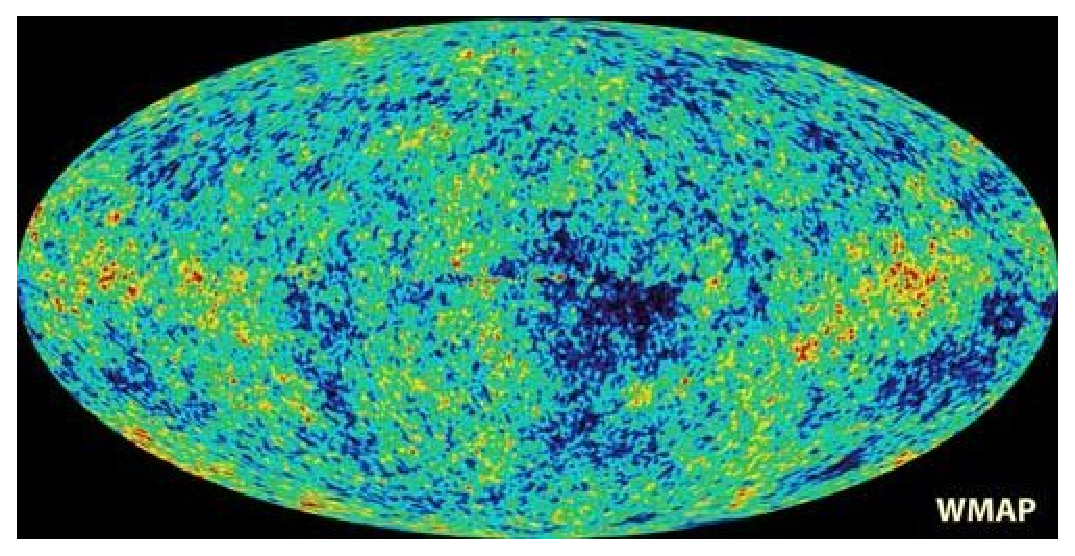
\includegraphics[width=1in]{pictures/wmap.eps}}
	\end{minipage}&
	\hspace{0.0in}
	\begin{minipage}[b]{2.4in}\textcolor{white}{%
	Close examination of slight CMB intensity variations in different parts of the sky help cosmologists study the formation of galaxies.
	\textcolor{gray}{WMAP photo by NASA}
	}
	\end{minipage}
	\end{tabular}
	}
	}
	}
}}
}


}

  %Title
  \rput[B]{0}(10.1,34.15){\titlefont \white The Electromagnetic Radiation Spectrum}

  %sine wave down the side of the poster
  \rput{270}(22.4,35.5){
  	\psplot[linestyle=solid,linewidth=2pt,fillstyle=none, linecolor=white, plotpoints=5000]{1}{36000}{3000000 div x mul x sin 4 div}
  }


{
  %Left side notes
  %Notes, table of conversions
  \psset{cornersize=absolute,linearc=4pt,fillstyle=solid,fillcolor=Black, linecolor=white}
  \white

  \rput[bl]{0}(12.6,22.15){
    \parbox[t]{4.8in}{

	\psframebox{\parbox[t]{4.8in}{\white{
\psset{linearc=0}
{\Large How to read this chart}
\begin{itemize}

\item This chart is organized in octaves (frequency doubling/halving) starting at 1Hz and going higher (2,4,8, etc) and lower (1/2, 1/4, etc). The octave is a natural way to represent frequency.

\item Frequency increases on the vertical scale in the upward direction.

\item The horizontal bars wrap around from far right to far left as the frequency increases upwards.

%\item This chart was also designed so that the spectrum section could be cut our and wrapped around a standard 3 inch diameter by 36 inches long mailing tube to represent a continuous frequency from the bottom to the top and beyond.

\item There is no limit to either end of this chart, however, due to limited space, only the ``known" items have been shown here. A frequency of 0Hz is the lowest possible frequency but the method of depicting octaves used here does not allow for ever reaching 0Hz, only approaching it. Also, by the definition of frequency (Cycles per second), there is no such thing as negative frequency.

\item Values on the chart have been labelled with the following colours: \psframebox[framesep=1pt,fillstyle=solid,fillcolor=Black]{\textcolor{FColor}{Frequency}}  measured in Hertz, \psframebox[framesep=1pt,fillstyle=solid,fillcolor=Black]{\textcolor{WColor}{Wavelength}} measured in meters, \psframebox[framesep=1pt,fillstyle=solid,fillcolor=Black]{\textcolor{EColor}{Energy}} measured in electronVolts.

\end{itemize}
}
}}

	\vspace{\VerticalSeparation}

	\psframebox{\parbox[t]{4.8in}{{\Large Ultraviolet Light}
\begin{itemize}
\item Ultraviolet light is just beyond the range of human vision.

\item Physicists have divided ultraviolet light ranges into Vacuum Ultraviolet (VUV), Extreme Ultraviolet (EUV), Far Ultraviolet (FUV), Medium Ultraviolet (MUV), and Near Ultraviolet (NUV).

\item UV-A, UV-B, and UV-C were introduced in the 1930's by the International Commission on Illumination (CIE) for photobiological spectral bands. UV-A is subdivided into UVA1 and UVA2, with the latter considered more harmful.


% possibly biased source for most of the below info: https://www.skincancer.org/prevention/uva-and-uvb
\item The sun produces a wide range of frequencies including all the ultraviolet light, however, UV-B is mostly filtered by the ozone layer and UV-C is entirely blocked by the earth's atmosphere.

\item UV-A makes up  95\% of the UV radiation reaching us from the sun and is the primary cause of skin-tanning. UV-B does not penetrate the deeper layers of the skin but plays a key role in sunburn, skin reddening, and skin cancer. UV-B is usually blocked by glass. UV-C is very harmful and is artifically generated for use as a germicide.

\item Ultraviolet ``blacklights`` used in theatres and nightclubs mostly emit invisible UV light in the 350-380nm range, though some visible purple light is also emitted. Phosphors absorb UV and re-emit visible light causing the characteristic blacklight glow. Your nails and teeth contain naturally occuring phosphors. Blacklights are very low energy and are not conisdered harmful in most situations.
% The natural UV-A in sunlight causes the same absorbption and re-emission of visible light, but this affect isn't noticed in the midst of other bright visible light. %%% <---- need to clean that up

% \item The CIE originally divided UVA and UVB at 315nm, later some photo-dermatologists divided it at 320nm.

\item Bumblebees can see into the UV-A range which helps them identify certain flowers.
\end{itemize}




% From: http://www.ping.at/cie/publ/abst/134-99.html
% Press Release:
% CIE Collection in Photobiology and Photochemistry, 1999
% CIE 134-1999 ISBN 3 900 734 94 1
% This volume contains short Technical Reports prepared by various Technical Committees within CIE Division 6.

% 134/1: TC 6-26 report: Standardization of the Terms UV-A1, UV-A2 and UV-B
% The terms UV-A, UV-B and UV-C were introduced in the 1930's by CIE Committee 41 on Ultraviolet Radiation as a short-hand notation for photobiological spectral bands. It was never intended that the bands were exclusive for different effects. The bands have been in widespread use in different medical fields and scientific research. UV-A and UV-B were divided at 315 nm by the CIE. In recent decades, some photo-dermatologists and others have used different dividing lines such as 320 nm without recognizing the importance of maintaining an international standardized terminology. Because the terminology is used in many fields, this report recommends that the 315 nm division between UV-A and UV-B be maintained. However, recent research has clearly shown a difference in the photobiological interaction of long and short wavelength UV-A radiation with DNA. This led to a further division of UV-A into UV-A1 and UV-A2 with a dividing line at approximately 340 nm. While this division may be of value, the committee does not recommend officially to split UV-A into these two sub-bands at this time. Further research may justify a dividing line different from 340 nm in the future.
}}

	\vspace{\VerticalSeparation}

	\psframebox{\parbox[t]{4.8in}{%Emission and Absorption lines
{\Large Emission and Absorption}
\begin{itemize}

%\item The fluorescent lamp uses luminescent material (phosphor) to convert ultraviolet radiation using photoluminescence into visible light. The phosphor absorbs UV light and emits visible light.

\item As EMR passes through elements, certain wavelength bands get absorbed and some new ones get emitted. This absorption and emission produces characteristic spectral lines for each element which are useful in determining the makeup of distant stars. These lines are used to prove the red-shift amount of distant stars.

\item
 When a photon hits an atom it may be absorbed if the energy is just right.
 The energy level of the electron is raised -- essentially holding the radiation.
 A new photon of specific wavelength is created when the energy is released.
 The jump in energy is a discrete step and many possible levels of energy exist in an atom.

\item Johann Balmer created this formula defining the photon emission wavelength ($\lambda$); where $m$ is the initial electron energy level and $n$ is the final electron energy level:

\hspace{1in}$\lambda = 364.56nm \left( \frac{\D m^2}{\D m^2 - n^2} \right)$

\item Much of the interstellar matter is made of the simplest atom hydrogen. The hydrogen visible-spectrum emission and absorption lines are shown below:

\end{itemize}

%what happens if the photons energy is slightly higher than required to elevate the electrons energy level? Where does the excess energy go after raising the electrons energy level?


%Start X, End X, Label, label offset
\newcommand{\absorbemit}[4]{
	\psframe(#1,.075)(#2,.165)
	\psline[linestyle=solid](#2,0)(#2,.083)
	\uput{2pt}[270](#2,#4){#3}
}
\vspace{0.2in}
\psframebox[fillstyle=none,linestyle=none]{
	\rput(0.1,0){
	%Start at 760nm (0in)
		\psset{xunit=.0120in,linestyle=none, linewidth=1pt, linecolor=Black, fillstyle=solid, fillcolor=Black,linearc=0}
{
%  Red 		760-620 nm
%  Orange 	620-570 nm
%  Yellow 	570-550 nm
%  Green 	550-470 nm
%  Blue 	470-440 nm
%  Violet 	440-380 nm
\psset{gradlines=100,fillstyle=gradient,gradangle=90,gradmidpoint=1.0,linewidth=0pt,linestyle=none}
\definecolor{StartColor}{hsb}{.0,1,1} \definecolor{EndColor}{hsb}{.1,1,1} \psframe[gradbegin=StartColor,gradend=EndColor](0,0)(165,.15) %Red to Orange
\definecolor{StartColor}{hsb}{.1,1,1} \definecolor{EndColor}{hsb}{.2,1,1} \psframe[gradbegin=StartColor,gradend=EndColor](165,0)(200,.15) %Orange to Yellow
\definecolor{StartColor}{hsb}{.2,1,1} \definecolor{EndColor}{hsb}{.38,1,1}\psframe[gradbegin=StartColor,gradend=EndColor](200,0)(250,.15) %Yellow to Green
\definecolor{StartColor}{hsb}{.4,1,1} \definecolor{EndColor}{hsb}{.5,1,1} \psframe[gradbegin=StartColor,gradend=EndColor](250,0)(305,.15) %Green to Blue
\definecolor{StartColor}{hsb}{.5,1,1} \definecolor{EndColor}{hsb}{.8,1,1} \psframe[gradbegin=StartColor,gradend=EndColor](305,0)(380.25,.15) %Blue to Violet
}
		\absorbemit{-2}{103.715}{$H_\alpha$}{0}
		\absorbemit{103.715}{273.867}{$H_\beta$}{0}
		\absorbemit{273.867}{325.953}{$H_\gamma$}{0}
		\absorbemit{325.953}{349.826}{$H_\delta$}{0}
		\absorbemit{349.826}{363.03}{$H_\epsilon$}{0}
		\absorbemit{363.03}{371.14}{$H_\zeta$}{-.13in}
		\absorbemit{371.14}{376.5}{$H_\eta$}{.32in}
		\absorbemit{376.5}{380.25}{$H_\theta$}{0}
		\absorbemit{380.25}{385}{}{0}
{
	\psset{linearc=2pt,linecolor=white,linestyle=solid,linewidth=1pt,fillstyle=none}
	\uput{2pt}[180](70,.17){Emission line}\psline{->}(70,.17)(86,.17)(86,.12)(102,.12)
	\uput{2pt}[180](70,-.10){Absorption line}\psline{->}(70,-.10)(86,-.10)(86,.04)(102,.04)
	\uput{2pt}[0](140,-.16){Balmer series name}\psline{->}(140,-.16)(127,-.16)(127,-.09)(113,-.09)
}
	}
}
\vspace{0.2in}

%longer at opposite end, must use negative co-ordinates (Ex. subtract from the beginning of red visible light 760nm )
%$H_\alpha$% 656.285nm  103.715
%$H_\beta$% 486.133nm 273.867
%$H_\gamma$% 434.047nm 325.953
%$H_\delta$% 410.174nm 349.826
%$H_\epsilon$% 396.97nm 363.03
%$H_\zeta$% 388.86nm 371.14
%$H_\eta$% 383.50nm 376.5
%$H_\theta$% 379.75nm 380.25

%from http://hyperphysics.phy-astr.gsu.edu/hbase/quantum/atspect.html#c1

%Emission
%Wavelength	Relative	Transition	Color
%(nm)		Intensity
%383.5384 	5 		9 -> 2 		Violet
%388.9049 	6 		8 -> 2 		Violet
%397.0072 	8 		7 -> 2 		Violet
%410.174 	15 		6 -> 2 		Violet
%434.047 	30 		5 -> 2 		Violet
%486.133 	80 		4 -> 2 		Bluegreen (cyan)
%656.272 	120 		3 -> 2 		Red
%656.2852 	180 		3 -> 2 		Red


\textcolor{gray}{\hrule}
\vspace{.4in}
\hspace{.3in}
\begin{tabular}{rl}
%blackbody radiation
\begin{minipage}[b]{1.1in}
	\psframebox[linestyle=none]{
		%
		%The following picture was created using the above Plank formula in a 
		% spreadsheet (balmer_series.gnumeric) then plotted.
		%The vertical scale is log(x), temperatures are 2000K, 1000K, 700K.
		\rput[bl](0,0){
\includegraphics{pictures/blackbody.eps}}
		%
		\psline[fillstyle=none, linearc=0]{<->}(1.1,0)(0,0)(0,.9)
		\rput[b]{90}(-.05,.45){Power}
		\rput[t](.5,-.05){Wavelength}
		\psset{border=1pt, bordercolor=Black, fillstyle=none, linearc=0,linecolor=green}
		\psline{o-}(.08,.6)(.5,.6)\uput{2pt}[0](.5,.6){White Hot}
		\psline{o-}(.12,.43)(.7,.43)\uput{2pt}[0](.7,.43){Red Hot}
		\psline{o-}(.18,.25)(.9,.25)\uput{2pt}[0](.9,.25){Hot}
		\psline{o-}(.7,0)(.88,.1)(1.05,.1)\uput{2pt}[0](1.05,.1){CMB}
	}
\end{minipage}&
\hspace{0.0in}
\begin{minipage}[b]{3in}
\begin{itemize}
\item Max Planck determined the relationship between the temperature of an object and its radiation profile; where $R_\lambda$ is the radiation power, $\lambda$ is the wavelength, $T$ is the temperature:

\hspace{.7in} $R_\lambda = \frac{\D 37418}{\D \lambda^5 \epsilon^{\left( \frac{\D 14388}{\D \lambda T}\D - 1 \right) }}$

\end{itemize}
\end{minipage}
\end{tabular}
\vspace{.15in}




%Fluorescent lamp 12,000K
%Sun 6,000K
%Incandescent lamp 3000K
%Cosmic Microwave Background radiation 3K

}}

	\vspace{\VerticalSeparation}

    }
  }

%   \rput[tl]{0}(12.6,19.31){
  \rput[tl]{0}(12.6,19.23){
    \parbox[t]{4.8in}{

	\psframebox{\parbox[t]{4.8in}{%TV text


%%% Update this to take into account the analog -> digital transition for TV transmissions
% - UHF tv bands only goes up to channel 38 now!
% - add in digital tv bands?

{\Large Television}
{
\definecolor{HumanAudioColor}{rgb}{0.2,0.2,0.6}
\begin{itemize}

\item Terrestrial broadcast TV uses the VHF and UHF ranges (30MHz - 3GHz)  \psframebox[linestyle=none]{\rput(0.05,.05){\psframebox[fillstyle=solid,framearc=0.25,fillcolor=red]{\textcolor{white}{\tiny 05}}}}\hspace{.1in}.

\item Satellite television is transmitted in the C-band (4 - 8 GHz)
\psframebox[linestyle=none]{\rput(0.05,.05){\psframebox[fillstyle=solid,framearc=.25,fillcolor=green]{\textcolor{black}{\tiny 05}}}}\hspace{.1in} and Ku-band (12 - 18 GHz)  \psframebox[linestyle=none]{\rput(0.04,0.02){\psdots[framesep=1pt,fillcolor=BrightGreen,fillstyle=solid,dotstyle=triangle,linecolor=BrightGreen](0,0)}}\hspace{.08in} where one of many satellites is shown. To eliminate interference, the stations are broadcast in alternating polarities, for example, Ch 1 is vertical and Ch 2 is horizontal and vice versa on neighbouring satellites.

%\item Each station is transmitted in its own band.
\item TV channels transmitted through cable (CATV) are shown as  \psframebox[linestyle=none]{\rput(0.05,.05){\psframebox[fillstyle=solid,framearc=0.1,fillcolor=blue]{\textcolor{white}{\tiny 05}}}}\hspace{.1in}. CATV channels starting with ``T-" are channels fed back to the cable TV station (like news feeds).
\item Air and cable analog TV stations are broadcast with the separate video, colour, and audio frequency carriers grouped together in a channel band as follows:\vspace{.31in}\\
	\psframebox[linestyle=none]{\psset{xunit=1.7in}
		\psline{|<->|}(0,.28)(2.5,.28)\uput{1pt}[90](1.25,.28){6MHz}
		\white
		\psframe[linestyle=solid,framearc=0.25,fillcolor=red,fillstyle=solid](0,0)(2.5,.25)
		\psdots[linecolor=white,dotstyle=triangle*](0.625,0.02)(1.915,0.02)(2.375,0.02)
		\psline[linecolor=white](0.625,0)(0.625,.25)
		\psline[linecolor=white](1.915,0)(1.915,.15)
		\psline[linecolor=white](2.375,0)(2.375,.25)
		\psline[linecolor=white]{<->}(0,.125)(.625,.125)\rput(.29,.125){
			\psframebox[linearc=1pt,linestyle=none,framesep=0pt,fillcolor=white,fillstyle=solid]{\textcolor{Black}{1.25MHz}}}
		\psline[linecolor=white]{<->}(.625,.07)(1.915,.07)\rput(1.27,.07){
			\psframebox[linearc=1pt,linestyle=none,framesep=0pt,fillcolor=white,fillstyle=solid]{\textcolor{Black}{3.58MHz}}}
		\psline[linecolor=white]{<->}(.625,.18)(2.375,.18)\rput(1.50,.18){
			\psframebox[linearc=1pt,linestyle=none,framesep=0pt,fillcolor=white,fillstyle=solid]{\textcolor{Black}{4.5MHz}}}
		\uput{1pt}[270](.625,0){Video}
		\uput{1pt}[270](1.915,0){Colour}
		\uput{1pt}[270](2.375,0){Audio}
		}\vspace{0.1in}

%TV horizontal refresh
\item 15.7 kHz horizontal sweep signal is a common contaminant to VLF listening \hspace{.05in}
  \psframebox[framearc=0,linearc=0]{\rput(0,.05){
	\psframe[cornersize=relative,linecolor=white, linestyle=solid, linewidth=0.8pt,fillstyle=solid,framearc=.25,fillcolor=red,linearc=0.25](-.1,-.1)(.1,.1)
	\psline[linecolor=white,linestyle=solid,linewidth=1pt]{<->}(-.1,0)(.1,0)
  }}\hspace{0.07in}.
\item Digital compression methods are used for HDTV broadcasts in order to pack more channels into the same 6MHz bandwidth as analog TV.

\end{itemize}

}



}}

	\vspace{\VerticalSeparation}

	\psframebox{\parbox[t]{4.8in}{%Radio description
{\Large Radio Bands}
%Draw a sinewave with
%	{Initial Amplitude x.xxx}{Initial Time-width x.xxx}{Initial Number of cycles x}
%	{Second Amplitude x.xxx}{Second Time-width x.xxx}{Second Number of cycles x}
%	{Total repeats}
\newlength{\nAmplitude}		\newlength{\nAmplitudeNeg}
\newlength{\nTime}		\newlength{\nTimeTwo}		\newlength{\nTimeThree}		\newlength{\nTimeFour}
\newlength{\nSAmplitude}	\newlength{\nSAmplitudeNeg}
\newlength{\nSTime}		\newlength{\nSTimeTwo}		\newlength{\nSTimeThree}	\newlength{\nSTimeFour}
\newlength{\nTimeEnd}		\newlength{\nSTimeEnd}		\newlength{\nSTimeStart}
\newcommand{\sinewave}[7]{
	\setlength{\nAmplitude}{#1}
	\setlength{\nAmplitudeNeg}{\nAmplitude*-1}
	\setlength{\nTime}{#2}
	\setlength{\nTimeTwo}{\nTime*2}
	\setlength{\nTimeThree}{\nTime*3}
	\setlength{\nTimeFour}{\nTime*4}
	\setlength{\nTimeEnd}{\nTime*4*#3}
	\setlength{\nSAmplitude}{#4}
	\setlength{\nSAmplitudeNeg}{\nSAmplitude*-1}
	\setlength{\nSTime}{#5}
	\setlength{\nSTimeTwo}{\nSTime*2}
	\setlength{\nSTimeThree}{\nSTime*3}
	\setlength{\nSTimeFour}{\nSTime*4}
	\setlength{\nSTimeEnd}{\nTime*4*#3+\nSTime*4*#6}
	\multido{\dXTimePosition=0.000in+\nSTimeEnd}{#7}{
		\multido{\dXPosition=\dXTimePosition+\nTimeFour}{#3}{
			\rput(\dXPosition,0){
			\parabola(0.00,0)(\nTime,\nAmplitude)\parabola(\nTimeTwo,0)(\nTimeThree,\nAmplitudeNeg)
			}
		}
		\setlength{\nSTimeStart}{\dXTimePosition+\nTimeEnd}
		\multido{\dXPosition=\nSTimeStart+\nSTimeFour}{#6}{
			\rput(\dXPosition,0){
			\parabola(0.00,0)(\nSTime,\nSAmplitude)\parabola(\nSTimeTwo,0)(\nSTimeThree,\nSAmplitudeNeg)
			}
		}
	}
}
%
\begin{itemize}

\item The radio spectrum (ELF to EHF) is populated by many more items than can be shown on this chart. Only a small sampling of bands used around the world have been shown.

\item Communication using EMR is done using either:
\begin{itemize}
\item Amplitude Modulation (AM)
%Amplitude Modulation
\psframebox[linestyle=none,fillstyle=none]{\rput(.1,0.05){\sinewave{.1in}{0.015in}{5}{.05in}{0.015in}{5}{4}}}\vspace{0.1in}\\
\vspace{0.04in}OR
\item Frequency Modulation (FM)
%Frequency Modulation
\psframebox[linestyle=none,fillstyle=none]{\rput(.1,0.05){\sinewave{.1in}{0.010in}{7}{.1in}{0.020in}{4}{4}}}
\vspace{0.1in}
\end{itemize}

\item Each country has its own rules and regulations for allotting bands in this region. Refer to the authority in your area (Ex. FCC in the USA, DOC in Canada).

\item Not all references agree on the ULF band range, the HAARP range is used here.

\item {\bfseries RA}dio {\bfseries D}etecting {\bfseries A}nd {\bfseries R}anging (RADAR) uses EMR in the microwave range to detect the distance and speed of objects.

\item {\bfseries C}itizens {\bfseries B}and Radio (CB) contains 40 stations between 26.965 - 27.405MHz.

\item Schumann resonance is produced in the cavity between the Earth and the ionosphere. The resonant peaks are depicted as \psframebox[fillstyle=none,linestyle=none]{\blip{0,-.07}{S}}

\item Hydrogen gas emits radio band EMR at 21cm \psframebox[fillstyle=none,linestyle=none]{\blip{0,-.07}{H}}

\item Some individual frequencies are represented as icons:\vspace{0.1in}\\
\begin{tabular}{cp{1.9in}cp{1.1in}}
\psframebox[linestyle=none]{\submarine{0.02,.05}{xxHz}}\hspace{0.2in}\vspace{0.05in} & Submarine communications&
\psframebox[linestyle=none]{\rput(0.15,.05)\pager}&Pager\\
\psframebox[linestyle=none]{\rput(0.15,.05){\timestandard}\hspace{.03in}}\vspace{0.05in} & Time / frequency standards&\psframebox[linestyle=none]{\rput(0.15,.05){\weatherstation}\hspace{.03in}\vspace{0.08in}} & Weather stations\\
\psframebox[linestyle=none]{\rput(0.14,0.01){\psframebox[fillstyle=solid,fillcolor=green,linecolor=green,linearc=0]{\textcolor{Black}{xxm}}}}\hspace{.1in}\vspace{0.05in} & Ham / international meter bands&
\psframebox[linestyle=none]{\rput(0.15,.04){
	\psframe[linestyle=solid,linecolor=gray,fillstyle=solid,fillcolor=gray,linearc=0](-.2,-.08)(.2,.08)
	\psframe[hatchwidth=2pt, hatchsep=1.5pt,linestyle=solid,linecolor=yellow,fillstyle=hlines,hatchangle=45,hatchcolor=yellow,fillcolor=gray,linearc=0](-.2,-.08)(.2,.08)
	}
	\hspace{.2in}}\vspace{0.05in}
 	& Short wave radio\\
\psframebox[linestyle=none]{\rput(0.05,.05){\psframebox[fillstyle=solid,fillcolor=Itinerant,linecolor=Itinerant,linearc=0,framesep=1pt]{\textcolor{Black}{GMRS}}}}&General Mobile Radio Service&
\psframebox[linestyle=none]{\rput(0.15,-0.05){\wirelessmic}}&Wireless Microphone\\
\psframebox[linestyle=none]{\rput(0.11,.05){\psframebox[fillstyle=solid,fillcolor=Itinerant,linecolor=Itinerant,linearc=0,framesep=1pt]{\textcolor{Black}{FRS}}}}&Family Radio Service&
\psframebox[linestyle=none]{\rput(0.15,.05){\psframebox[fillstyle=solid,linearc=0,linecolor=yellow,framesep=1pt,fillcolor=yellow,linewidth=1pt,linestyle=solid]{\textcolor{Black}{CP}}}\hspace{.03in}\vspace{0.08in}} & Cellular Phones\\
\psframebox[linestyle=none]{\rput(0.11,.05){\psframebox[linestyle=none,framesep=1pt,fillcolor=red,linearc=0]{\white SOS}}}&
	\psset{dotsize=1pt 1}Distress signal, in Morse code:\vspace{0.18in}
\rput(-1.4,-0.18){\rput(0,0.05){\psdots(0,0)(.1,0)(.2,0)\psline{cc-cc}(0.3,0)(0.42,0)\psline{cc-cc}(0.49,0)(0.61,0)\psline{cc-cc}(0.68,0)(0.8,0)\psdots(.9,0)(1,0)(1.1,0)}}&\hspace{0.1in}&\hspace{0.1in}\\
\end{tabular}

\end{itemize}
}}

    }
  }

  %\rput[tl]{0}(15.6,14){\psframebox{\parbox[t]{2.3in}{%NOAA Weather Radio Frequencies

{
\centering

NOAA Weather Radio Frequencies\\
\begin{tabular}{|l|}\hline
162.400  MHz *      \\
162.425  MHz        \\
162.450  MHz        \\
162.475  MHz *      \\
162.500  MHz        \\
162.525  MHz        \\
162.550  MHz *      \\
\hline
\end{tabular}\\

* most common

}

}}}
  %\rput[tl]{0}(15.4,15.8){\psframebox\parbox[t]{2.1in}{%Satellite signal table

{

\centering

Satellite TVRO Bands\\
\begin{tabular}{|c|c|}\hline
Band     & Frequency range      \\ \hline
S-Band   & 1700-3000 MHz        \\
C-Band   & 3700-4200 MHz        \\
Ku1-Band & 10.9-11.75 GHz       \\
Ku2-Band & 11.75-12.5 GHz (DBS) \\
Ku3-Band & 12.5-12.75 GHz       \\
Ka-Band  & 18.0-20.0 GHz        \\
\hline
\end{tabular}\\

\vspace{0.1in}

Satellite Downlink Frequency Assignments\\
\begin{tabular}{|c|c|}\hline
Band     & Frequency range          \\ \hline
C-Band downlink   & 3.4-4.8 GHz     \\
Ku-Band downlink  & 10.7-12.75 GHz  \\
\hline
\end{tabular}\\

}
}}}
  %\rput[tl]{0}(18.1,19.4){\psframebox{\parbox[t]{1.3in}{%Citizen's Band Radio

{ \scriptsize
\centering

Citizen's Band (CB) Radio\\
\begin{tabular}{|c|c|}\hline
Channel     & Frequency \\ \hline
01 & 26.965 MHz        \\
02 & 26.975 MHz        \\
03 & 26.985 MHz        \\
04 & 27.005 MHz        \\
05 & 27.015 MHz        \\
06 & 27.025 MHz        \\
07 & 27.035 MHz        \\
08 & 27.055 MHz        \\
09 & 27.065 MHz        \\
10 & 27.075 MHz        \\
11 & 27.085 MHz        \\
12 & 27.105 MHz        \\
13 & 27.115 MHz        \\
14 & 27.125 MHz        \\
15 & 27.135 MHz        \\
16 & 27.155 MHz        \\
17 & 27.165 MHz        \\
18 & 27.175 MHz        \\
19 & 27.185 MHz        \\
20 & 27.205 MHz        \\
21 & 27.215 MHz        \\
22 & 27.225 MHz        \\
23 & 27.255 MHz        \\
24 & 27.235 MHz        \\
25 & 27.245 MHz        \\
26 & 27.265 MHz        \\
27 & 27.275 MHz        \\
28 & 27.285 MHz        \\
30 & 27.305 MHz        \\
31 & 27.315 MHz        \\
32 & 27.325 MHz        \\
33 & 27.335 MHz        \\
34 & 27.345 MHz        \\
35 & 27.355 MHz        \\
36 & 27.365 MHz        \\
37 & 27.375 MHz        \\
38 & 27.385 MHz        \\
29 & 27.295 MHz        \\
39 & 27.395 MHz        \\
40 & 27.405 MHz        \\

\hline
\end{tabular}\\

\vspace{0.05in}

}
}}}

  \rput[tl]{0}(13.4,10.5){
    \parbox[t]{4in}{

	%Description of Sound
	\psframebox{\parbox[t]{4in}{{\Large Sound}
{
\definecolor{HumanAudioColor}{rgb}{0.2,0.2,0.6}
%
\begin{itemize}

\item Although sound, ocean waves, and heartbeats are not electromagnetic, they are included on this chart as a frequency reference. Other properties of electromagnetic waves are different from sound waves.

\item Sound waves are caused by an oscillating compression of molecules. Sound cannot travel in a vacuum such as outer space.

\item The speed of sound in air at sea level is 1240kph (770mph).

\item Humans can only hear sound between $\approx$20Hz to $\approx$20kHz.

\item Infrasound (below 20Hz) can be sensed by internal organs and touch.
%
%from http://www.worldtravelers.org/motionsickness.htm
Frequencies in the 0.2Hz range are often the cause of motion sickness.

\item Bats can hear sound up to $\approx$50kHz.

\item The 88 piano keys of the Equal Temperament scale are accurately located on the frequency chart.

\item Over the ages people have striven to divide the continuous audio frequency spectrum into individual musical notes that have harmonious relationships. Microtonal musicians study various scales. One recent count lists 4700 different musical scales.

\item The musical note A is depicted on the chart as \pscirclebox[fillstyle=solid,fillcolor=HumanAudioColor]{\textcolor{white}{A}}

\textcolor{gray}{\hrule}
\vspace{.1in}

%\item This image depicts air being compressed as sound waves in a tube from a speaker and then travelling through the tube towards the ear.\\
%%picture of sound
%\vspace{1.75in}
%\rput[t]{0}(1,-.5){%Description: Sound wave schematic travelling through air

\psset{unit=0.5in}

\psset{viewpoint=1 -1 1}

\definecolor{EarColour}{rgb}{1,0.8,0.8}

%Draw speaker
\ThreeDput[normal=1 0 0](0,0,0){
	\pscircle[fillstyle=solid,fillcolor=red,linecolor=red](0,0){0.4}
	}


\input{pictures/waves.tex}

% Speaker label
\ThreeDput[normal=0 -1 0]{
	\uput{0.2in}[180](0,0){\white Speaker}
	}

%Draw ear
\ThreeDput[normal=1 0 0](5,0,0){
	\pscircle[fillstyle=solid,fillcolor=EarColour,linecolor=gray](0,0){0.4}
	}



% Ear label
\ThreeDput[normal=1 0 0](5,0,0){
	\rput(0,0){Ear}
	}
}
\end{itemize}
	\vspace{0.1in}
	%
	\begin{tabular}{rl}
	%\begin{minipage}[b]{2.45in}\rput(.65,1){%Description: Sound wave schematic travelling through air

\psset{unit=0.5in}

\psset{viewpoint=1 -1 1}

\definecolor{EarColour}{rgb}{1,0.8,0.8}

%Draw speaker
\ThreeDput[normal=1 0 0](0,0,0){
	\pscircle[fillstyle=solid,fillcolor=red,linecolor=red](0,0){0.4}
	}


\input{pictures/waves.tex}

% Speaker label
\ThreeDput[normal=0 -1 0]{
	\uput{0.2in}[180](0,0){\white Speaker}
	}

%Draw ear
\ThreeDput[normal=1 0 0](5,0,0){
	\pscircle[fillstyle=solid,fillcolor=EarColour,linecolor=gray](0,0){0.4}
	}



% Ear label
\ThreeDput[normal=1 0 0](5,0,0){
	\rput(0,0){Ear}
	}
}
	\begin{minipage}[b]{2.45in}\rput(1.3,.55){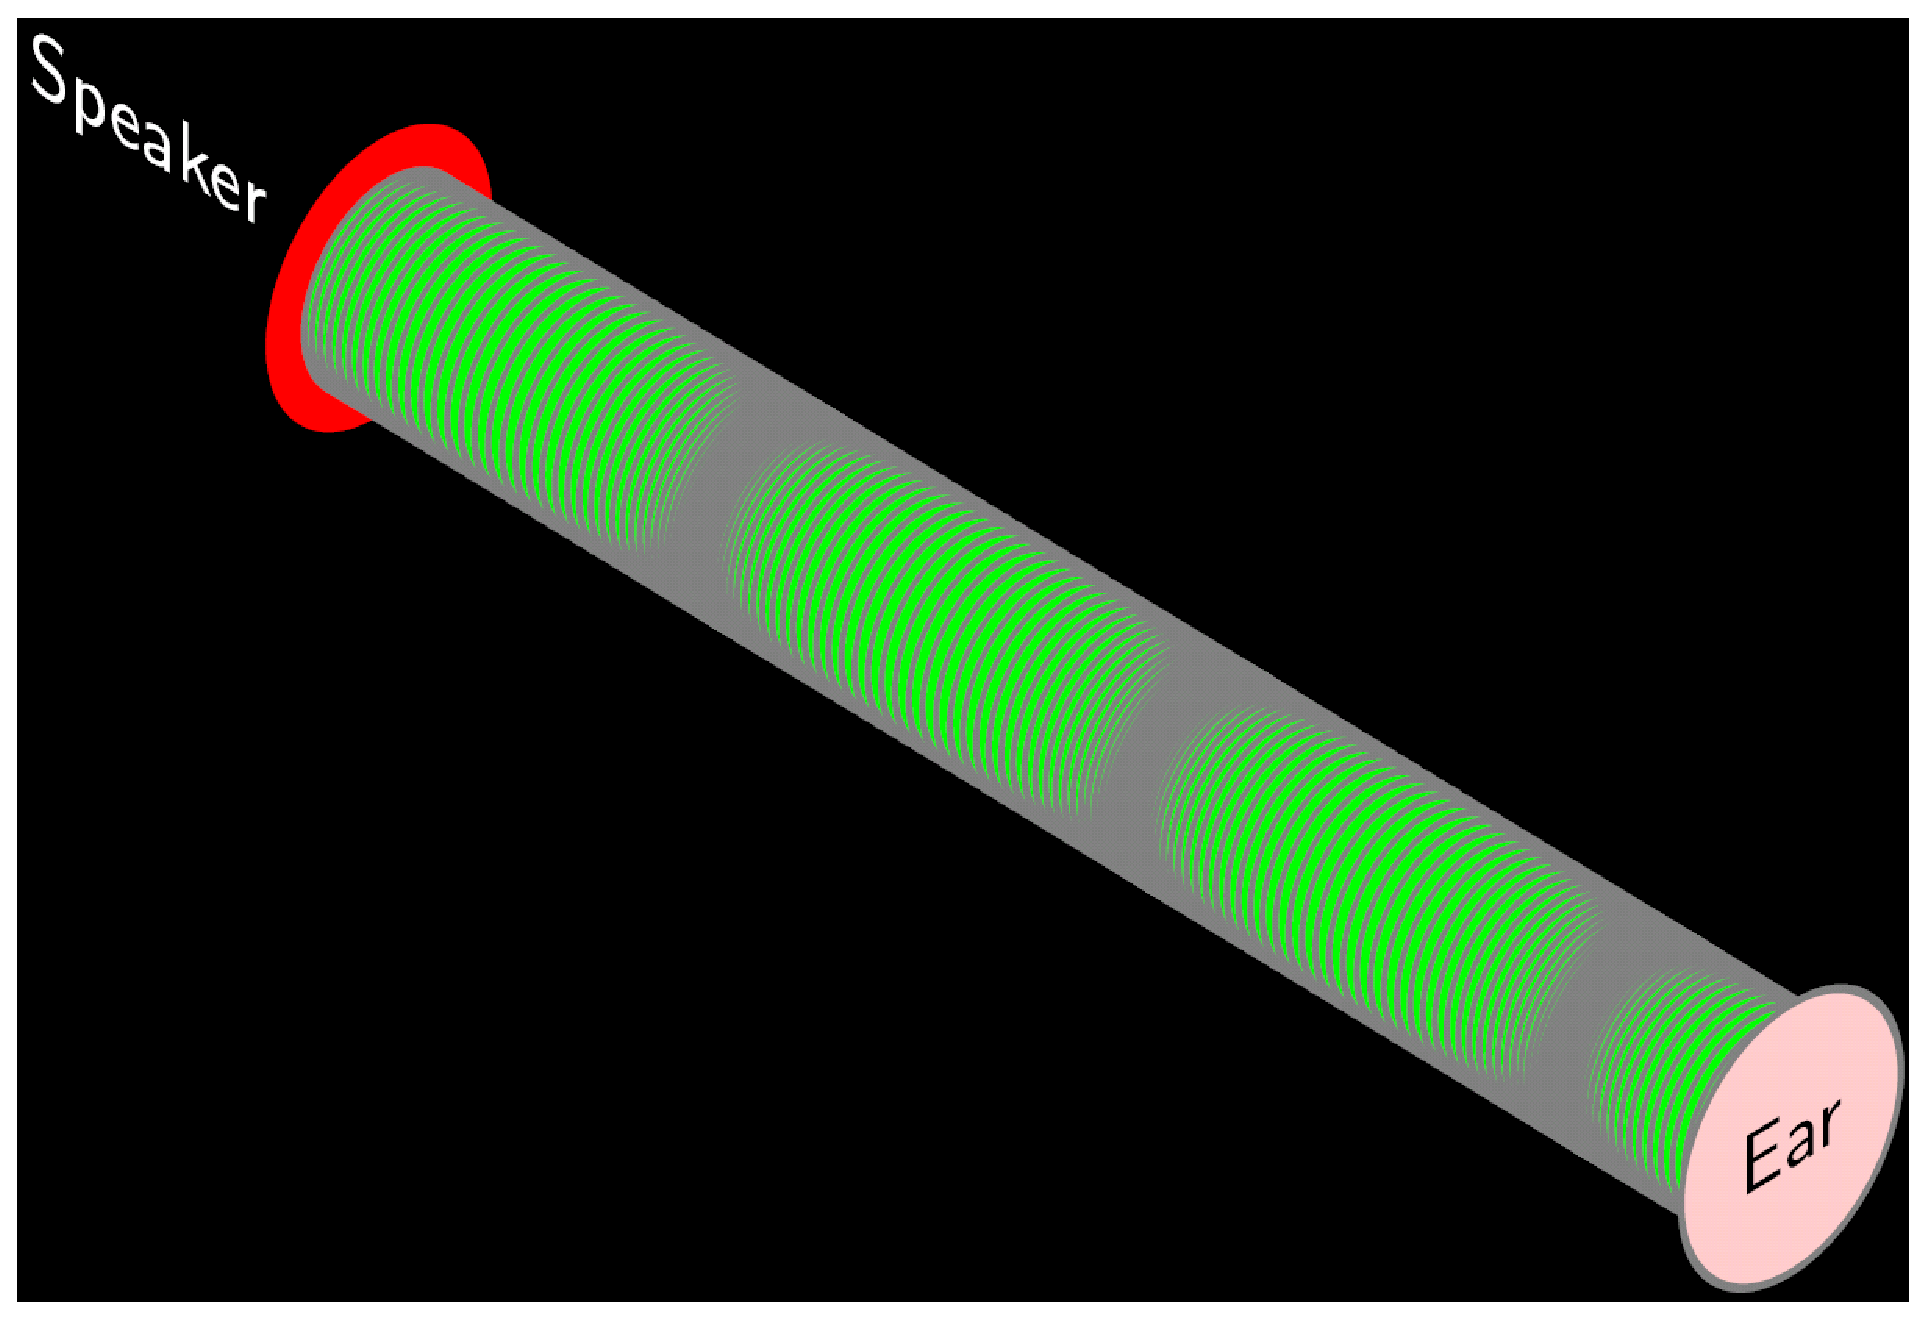
\includegraphics[width=2.2in]{pictures/soundbmp.eps}}
	\end{minipage}&
	\hspace{0.0in}
	\begin{minipage}[b]{1.2in}\textcolor{white}{%
	This image depicts air being compressed as sound waves in a tube from a speaker and then travelling through the tube towards the ear.\\	}
	\end{minipage}
	\end{tabular}
	\vspace{.2in}
}
}}

	\vspace{\VerticalSeparation}

	%Description of Gravity and gravity waves
	\psframebox{\parbox[t]{4in}{{\white

{\Large Gravitational Waves}

\begin{itemize}

\item Gravity is the mysterious force that holds large objects together and binds our planets, stars, and galaxies together. Many people have unsuccessfully theorized about the details of gravity and its relationship to other forces. There have been no links between gravity waves and electromagnetic radiation.

\item Gravity is theorized to warp space and time. In fact, gravity is responsible for bending light as observed by the gravity-lens example of distant galaxies.

\item ``Gravitational waves" would appear as ripples in space-time formed by large objects moving through space that might possibly be detected in the future by very sensitive instruments.

\item The speed that gravity propagates through space has not yet been been determined.

\end{itemize}
}

}}

	\vspace{\VerticalSeparation}

	%Description of Brain waves
	\psframebox{\parbox[t]{4in}{{\Large Brain Waves}
\begin{itemize}
\item By connecting electrodes from the human head to an electroencephalograph (EEG), it is possible to measure very small cyclic electrical signals.
\item There has been much study on this topic, but like all effects on humans, the findings are not as sound as the science of materials.
\item Generally, lower brain wave frequencies relate to sleep, and the higher frequencies relate to alertness.
\item Devices have been made for measuring and stimulating brain waves to achieve a desired state.
\end{itemize}
}}
    }
  }
}



\rput[bl]{0}(17.8,-.55){\white
  	\parbox[t]{4in}{
\psset{cornersize=absolute,linearc=4pt,fillstyle=solid,fillcolor=Black, linecolor=white}

	\psframebox{\parbox[t]{4in}{{\Large {\bfseries E}lectro{\bfseries m}agnetic {\bfseries R}adiation (EMR)}
\begin{itemize}
\item EMR is emitted in discrete units called photons but has properties of waves as seen by the images below. EMR can be created by the oscillation or acceleration of electrical charge or magnetic field. EMR travels through space at the speed of light (2.997 924 58 $\times 10^{8}$ \metrepersecond ). EMR consists of an oscillating electrical and magnetic field which are at right angles to each other and spaced at a particular wavelength.
% There is some controversy about the phase relationship between the electrical and magnetic fields of EMR, one of the theoretical representations is shown here:
%Continuous electromagnetic radiation represented as a wave.

\rput[t]{0}(0.5,-.8){%Description: Electromagnetic radiation schematic with travelling photon

\definecolor{DarkGreen}{rgb}{0,0.6,0}
\definecolor{MagneticBlue}{rgb}{.7,.7,1}
\definecolor{ElectricRed}{rgb}{1,.7,.7}

\psset{unit=0.5in}

\psset{viewpoint=1 1 1}

\psset{hatchsep=2pt}

%Axis labels
\ThreeDput[normal=1 0 0 ]{\textcolor{ElectricRed}{
       \psline[linecolor=ElectricRed]{<->}(0,-1.5)(0,1.5)
       \uput{2pt}[90](0,1.5){+E}
       \uput{2pt}[270](0,-1.5){-E}}
}

\ThreeDput[normal=0 0 1,embedangle=90]{\textcolor{MagneticBlue}{
	\psline[linecolor=MagneticBlue]{<->}(0,-1.5)(0,1.5)
	\uput{2pt}[270](0,-1.5){+B}
	\uput{2pt}[90](0,1.5){-B}}
}



%% In-phase magnetic (all three humps)
\ThreeDput[normal=0 0 1,embedangle=90]{
	\psset{linestyle=none, fillstyle=hlines,hatchangle=90,hatchcolor=MagneticBlue}
	\parabola(0,0)(.5,-1)
	\parabola(1,0)(1.5,1)
	\parabola(2,0)(2.5,-1)
      }

%% Out-of-phase magnetic (first half-hump)
% \ThreeDput[normal=0 0 1,embedangle=90]{
% 	\psset{linestyle=none, fillstyle=hlines,hatchangle=90,hatchcolor=MagneticBlue}
% 	\psclip{\psframe[linestyle=none, fillstyle=none](0,0)(0.5,-1)}
% 	\parabola(-0.5,0)(0,-1)
% 	\endpsclip	
%        }
%% Out-of-phase magnetic (second hump)
% \ThreeDput[normal=0 0 1,embedangle=90]{
% 	\psset{linestyle=none, fillstyle=hlines,hatchangle=90,hatchcolor=MagneticBlue}
% 	\parabola(0.5,0)(1,1)
%        }

\ThreeDput[normal=1 0 0]{
	\psset{linestyle=none, fillstyle=hlines,hatchangle=90,hatchcolor=ElectricRed}
	\parabola(0,0)(.5,1)
       }

%% Out-of-phase magnetic (fourth half-hump)
% \ThreeDput[normal=0 0 1,embedangle=90]{
% 	\psset{linestyle=none, fillstyle=hlines,hatchangle=90,hatchcolor=MagneticBlue}
% 	\psclip{\psframe[linestyle=none, fillstyle=none](2.5,0)(3,1)}
% 	\parabola(2.5,0)(3,1)
% 	\endpsclip	
%        }

\ThreeDput[normal=1 0 0]{
	\psset{linestyle=none, fillstyle=hlines,hatchangle=90,hatchcolor=ElectricRed}
	\parabola(1,0)(1.5,-1)
       }

%% Out-of-phase magnetic (third hump)
% \ThreeDput[normal=0 0 1,embedangle=90]{
% 	\psset{linestyle=none, fillstyle=hlines,hatchangle=90,hatchcolor=MagneticBlue}
% 	\parabola(1.5,0)(2,-1)
%        }



\ThreeDput[normal=1 0 0]{
	\psset{linestyle=none, fillstyle=hlines,hatchangle=90,hatchcolor=ElectricRed}
	\parabola(2,0)(2.5,1)
       }

%%Draw photon
%\ThreeDput[normal=1 -1 1](4,0,0){
%	\pscircle[fillstyle=solid,fillcolor=DarkGreen,linecolor=DarkGreen](0,0){0.1}
%	\psarc[linestyle=solid,linecolor=white,linewidth=0.5pt]{cc-cc}(0,0){0.065}{100}{150}
%	}

% Space label
\ThreeDput[normal=1 0 0]{
       \psline[linecolor=white,linestyle=solid]{cc->}(0,0)(3.4,0)
       \uput{5pt}[180](0,0){\white Source}
       \uput{4pt}[270](2.8,0){\white Space}
       }


\rput[l](-1,-2.2){\parbox[t]{2in}{
	\textcolor{ElectricRed}{E = Electric Field Strength}\\
	\textcolor{MagneticBlue}{B = Magnetic Field Strength}\\
	\textcolor{white}{Wave Nature}}}

}
\rput[t]{0}(2.8,-.8){%Description: Electromagnetic radiation schematic with travelling photon

\definecolor{DarkGreen}{rgb}{0,0.6,0}
\definecolor{MagneticBlue}{rgb}{.7,.7,1}
\definecolor{ElectricRed}{rgb}{1,.7,.7}

\psset{unit=0.5in}

\psset{viewpoint=1 1 1}

\psset{hatchsep=2pt}

%Axis labels
\ThreeDput[normal=1 0 0 ]{\psline[linecolor=ElectricRed]{<->}(0,-1.5)(0,1.5)}

\ThreeDput[normal=0 0 1,embedangle=90]{\psline[linecolor=MagneticBlue]{<->}(0,-1.5)(0,1.5)}


% Source and Space label
\ThreeDput[normal=1 0 0]{
       \psline[linecolor=white,linestyle=solid]{cc->}(0,0)(1.65,0)
       \uput{5pt}[180](0,0){\white Source}
       \uput{4pt}[270](1,0){\white Space}
       }

%Draw photon (position approximate since THREED system is confusing and circle must not be squashed)
\rput(1.3,-.74){
	\pscircle[fillstyle=solid,fillcolor=DarkGreen,linecolor=DarkGreen](0,0){0.1}
	\psarc[linestyle=solid,linecolor=white,linewidth=0.5pt]{cc-cc}(0,0){0.065}{100}{150}
	}

\rput[l](-1,-2.2){\parbox[t]{2in}{
	\textcolor{white}{Particle Nature}}}

}

\vspace{2.2in}

\item The particle nature of EMR is exhibited when a solar cell emits individual electrons when struck with very dim light.

\item The wave nature of EMR is demonstrated by the famous double slit experiment that shows cancelling and addition of waves.

\item Much of the EMR properties are based on theories since we can only see the effects of EMR and not the actual photon or wave itself.

\item Albert Einstein theorized that the speed of light is the fastest that anything can travel. So far he has not been proven wrong.

\item EMR can have its wavelength changed if the source is receding or approaching as in the red-shift example of distant galaxies and stars that are moving away from us at very high speeds. The emitted spectral light from these receding bodies appears more red than it would be if the object was not moving away from us.

\item We only have full electronic control over frequencies in the microwave range and lower. Higher frequencies must be created by waiting for the energy to be released from elements as photons. We can either pump energy into the elements (ex. heating a rock with visible EMR and letting it release infrared EMR) or let it naturally escape (ex. uranium decay).

\item We can only see the visible spectrum. All other bands of the spectrum are depicted as hatched colours \psframebox[fillstyle=none,linestyle=none,framesep=0in]{\psframe[linearc=0,framearc=0,fillstyle=crosshatch,linewidth=0pt,linestyle=none, hatchwidth=2pt, hatchsep=1.5pt,hatchcolor=white](0,-.04)(.4,.1)}\hspace{0.4in}.


\end{itemize}
}}

	\vspace{\VerticalSeparation}

	%description of How to read this chart
	\psframebox{\parbox[t]{4in}{%Notes:

%  Symbols here require \usepackage{SIunits}

{\centering

\begin{tabular}{|c|c|l|l|}\hline
\multicolumn{4}{|c|}{\bfseries  Syst�me International d'unit� prefixes (SI unit prefixes)}\\ \hline
Symbol & Name & Exp. & Multiplier\\ \hline
\rule[0mm]{0mm}{4mm}\yotta& yotta   & \yottad  & 1,000,000,000,000,000,000,000,000\\
\zetta& zetta   & \zettad  & 1,000,000,000,000,000,000,000\\
\exa& exa   & \exad  & 1,000,000,000,000,000,000\\
\peta& peta  & \petad  & 1,000,000,000,000,000\\
\tera& tera  & \terad  & 1,000,000,000,000\\
\giga& giga  & \gigad   & 1,000,000,000\\
\mega& mega  & \megad   & 1,000,000\\
\kilo& kilo  & \kilod   & 1,000\\
 &       & $10^{0}$   & 1\\
\milli& milli & \millid  & 0.001\\
\micro& micro & \microd  & 0.000 001\\
\nano& nano  & \nanod  & 0.000 000 001\\
\pico& pico  & \picod & 0.000 000 000 001\\
\femto& femto & \femtod & 0.000 000 000 000 001\\
\atto& atto  & \attod & 0.000 000 000 000 000 001\\
\zepto& zepto & \zeptod & 0.000 000 000 000 000 000 001\\
\yocto& yocto & \yoctod & 0.000 000 000 000 000 000 000 001\\
\hline
\end{tabular}\\

\vspace{0.1in}

\begin{tabular}{|c|c|c|}\hline
\multicolumn{3}{|c|}{\bfseries Measurements on this chart}\\ \hline
Symbol     & Name                          & Value                                             \\ \hline
\rule[0mm]{0mm}{4mm}$c$        & Speed of Light                & 2.997 924 58 $\times 10^{8}$ \metrepersecond      \\
$h$        & Planck's Constant             & 6.626 1 $\times 10^{-34}$  \joule$\cdot$\second   \\
$\hbar$    & Planck's Constant (freq)      & 1.054 592 $\times 10^{-34}$  \joule$\cdot$\second \\
\textcolor{FColor}{$f$}        & Frequency (cycles / second) & Hz                                                \\
\textcolor{WColor}{$\lambda$}  & Wavelength (meters)           & \metre                                            \\
\textcolor{EColor}{$E$}        & Energy (Joules)               & J                                                 \\
\hline
\end{tabular}\\

\vspace{0.1in}
}
{

\centering

%%Conversions:\\
%\fbox{\parbox{1.6in}{\begin{eqnarray}
%  E             &=& h \cdot f          \nonumber\\
%  \lambda       &=& \frac{c}{f}        \nonumber\\
%  1\angstrom    &=& 0.1\nano\metre     \nonumber\\
%  1\nano\metre  &=& 10\angstrom        \nonumber\\
%  1Joule        &=& 6.24 \times 10^{18} \electronvolt \nonumber
%\end{eqnarray}}
%}
% FColor
% WColor
% EColor

\parbox{1in}{\centering
\setlength{\tabcolsep}{2pt}
\hspace{0.4in}\begin{tabular}{|rcl|}\hline
\multicolumn{3}{|c|}{\bfseries Formulas}\\ \hline
  {\textcolor{EColor}{$E$}}        &=& $h \cdot \textcolor{FColor}{f}$\rule[0.1in]{0in}{0.01in}          \\
  {\textcolor{WColor}{$\lambda$}}   &=& $\frac{\D c}{\D \textcolor{FColor}{f}}$\rule[-0.1in]{0in}{0.15in}\\
  {\textcolor{FColor}{$f$}}         &=& $\frac{\D c}{\D \textcolor{WColor}{\lambda}}$\rule[-0.1in]{0in}{0.15in} \\ \hline
\end{tabular}}\hfill\parbox{2in}{\centering
\setlength{\tabcolsep}{2pt}
\begin{tabular}{|rcl|}\hline
\multicolumn{3}{|c|}{\bfseries Conversions}\\ \hline
  \rule{0in}{0.15in}1\angstrom    &=& 0.1\nano\metre     \\
  1\nano\metre  &=& 10\angstrom        \\
  1Joule        &=& 6.24 $\times 10^{18}$ \electronvolt \\ \hline
\end{tabular}}\vspace{0.07in}

%\begin{tabular}{|rcl|}\hline
%\multicolumn{3}{|c|}{\bfseries Conversions}\\ \hline
%  E             &=&
%  E             &=&
%  $f$     &=& $\frac{\D 2.997 924 58 $\times 10^{8}$}{\D \lambda}$        \\
%  $f$     &=&
%  $\lambda$     &=& $\frac{\D 2.997 924 58 $\times 10^{8}$}{\D f}$        \\
%
%  $\lambda$     &=&
%
%\end{tabular}\\

}



}}

	\vspace{\VerticalSeparation}

	\psframebox{\parbox[t]{4in}{\white%gammarays
{\Large Gamma Rays}
\begin{itemize}

\item Gamma radiation is the highest energy radiation (up to $\approx 10^{20}$ eV) that has been measured. At this energy, the radiation could be from gamma-rays, protons, electrons, or something else.

\item Alpha, beta, and delta radiation are not electromagnetic but are actually parts of the atom being released from a radioactive element. In some cases this can cause gamma radiation. These are not to be confused with brain waves of similar names.

\end{itemize}
}}

	\vspace{\VerticalSeparation}

	\psframebox{\parbox[t]{4in}{\white{\psset{gradlines=100,
 fillstyle=gradient,
 gradangle=90,
 gradmidpoint=1.0,
 linewidth=0pt,
 linestyle=none,
 linearc=0pt}
{\Large Visible Spectrum \hspace{0.05in}
	\psframebox[fillstyle=none,linestyle=none]{\psset{xunit=2.8in}
		\multido{%
			\nStartColor=0.00+0.1,
			\nEndColor=0.1+0.1,
			\nLeftSide=0.00+0.10,
			\nRightSide=0.10+0.10}{8}{%
			\definecolor{StartColor}{hsb}{\nStartColor,1,1}
			\definecolor{EndColor}{hsb}{\nEndColor,1,1}
			\psframe[fillstyle=gradient,
				gradangle=90,
				gradbegin=StartColor,
				gradend=EndColor,
				gradmidpoint=1.0,
				linewidth=0pt,
				linestyle=none]
			(\nLeftSide,0)(\nRightSide,0.15)}
			}
}
\begin{itemize}

\item The range of EMR visible to humans is called ``Light". The visible spectrum also closely resembles the range of EMR that filters through our atmosphere from the sun.

\item Other creatures see different ranges of visible light; for example bumble-bees can see ultraviolet light and dogs have a different response to colours than do humans.

\item The sky is blue because our atmosphere scatters light and the shorter wavelength blue gets scattered the most. It appears that the entire sky is illuminated by a blue light but in fact that light is scattered from the sun. The longer wavelengths like red and orange move straight through the atmosphere which makes the sun look like a bright white ball containing all the colours of the visible spectrum.

\item Interestingly, the visible spectrum covers approximately one octave.

\item Astronomers use filters to capture specific wavelengths and reject unwanted wavelengths. The major astronomical (visual) filter bands are depicted as  \psframebox[fillstyle=none,linestyle=none]{\astrofilter{0.07,0.03}{X}}

\end{itemize}
}
}}

	\vspace{\VerticalSeparation}

	\psframebox{\parbox[t]{4in}{{\Large Infrared Radiation}
\begin{itemize}

\item Infrared radiation (IR) is sensed by humans as heat and is below the range of human vision. Humans (and anything at room temperature) are emitters of IR.

\item IR remote control signals are invisible to the human eye but can be detected by most camcorders.

\item Night vision scopes/goggles use a special camera that senses IR and converts the image to visible light. Some IR cameras employ an IR lamp to help illuminate the view.

\item IR LASERs are used for burning objects.

\item A demonstration of IR is to hold a metal bowl in front of your face. The IR emitted by your body  will be reflected back using the parabolic shape of the bowl and you will feel the heat.

%Information provided by Edward  Alan Dowdell:
%http://www.fiber-optics.info/fiber-history.htm
%http://www.thefoa.org/tech/wavelength.htm
%http://www.webopedia.com/TERM/E/EDFA.html
\item Fiber-optic based infrared communication signals are sometimes amplified with Erbium-Doped Fiber Amplifiers  \scalebox{.8}{\psframebox[linestyle=none]{\fiberoptics{0.13,-.13}{EDFA}}}
\end{itemize}
}}

	\vspace{\VerticalSeparation}

	\psframebox{\parbox[t]{4in}{{\Large LASER}
\begin{itemize}

\item LASER is an acronym for {\bfseries L}ight {\bfseries A}mplification by {\bfseries S}timulated {\bfseries E}mission of {\bfseries R}adiation.
\item A LASER is a device that produces monochromatic EMR of high intensity.
\item With proper equipment, any EMR can be made to operate like a LASER. For example, microwaves are used to create a MASER.

%\item Junk/reword: Photons can be brought together and the resultant sum of forces is seen. If the polarization and phase are the same for the photons the the resultant light appears to be amplified. Some LASERs achieve this by constantly pumping photons into a filter to get the same frequency then bouncing those filtered photons off opposing mirrors to get the phase and polarization just right. Once the light has been ``amplified" enough it will escape from one of the mirrors.

\end{itemize}
}}

	\vspace{\VerticalSeparation}

	\psframebox{\parbox[t]{4in}{{\Large Polarization}
\begin{itemize}

\item As a photon (light particle) travels through space, its axis of electrical and magnetic fluctuations does not rotate. Therefore, each photon has a fixed linear polarity of somewhere between 0\degree\ to 360\degree. Light can also be circularly and elliptically polarized.

\item Some crystals can cause the photon to rotate its polarization.

\item Receivers that expect polarized photons will not accept photons that are in other polarities. (ex.\ satellite dish receivers have horizontal and vertical polarity positions).

\item A polarized filter (like Polaroid\texttrademark\  sunglasses) can be used to demonstrate polarized light. One filter will only let photons that have one polarity through. Two overlapping filters at right angles will almost completely block the light that exits; however, a third filter inserted between the first two at a 45\degree\ angle will rotate the polarized light and allow some light to come out the end of all three filters.

\item Light that reflects off an electrical insulator becomes polarized. Conductive reflectors do not polarize light.

% from Doug Welch
\item Perhaps the most reliably polarized light is a rainbow.

\item Moonlight is also slightly polarized. You can test this by viewing the moonlight through a Polaroid\texttrademark sunglass lens, then rotate that lens, the moonlight will dim and brighten slightly.

\end{itemize}


}}

	\vspace{\VerticalSeparation}

	\psframebox{\parbox[t]{4in}{%Refraction
{
\psset{linestyle=none}
\textcolor{white}{\Large Refraction}

\begin{itemize}
\item Refraction of EMR is dependent on wavelength as can be seen by the prism example below.
\end{itemize}

\begin{tabular}{cl}
%Prism
\begin{minipage}[b]{1.8in}
\includegraphics{pictures/prism.eps}
\end{minipage}&
\hspace{0.0in}
\begin{minipage}[b]{1.8in}\textcolor{white}{%
	By using a glass prism, white light can be
	spread by refraction into a spectrum of its composite colours.
	All wavelengths of EMR can be refracted by using the proper materials.
	Not all glass prisms behave alike; a right-angle prism will act as a mirror instead of a light refractor.  The critical angle of a true light-refracting prism is 42\degree.
	}
\end{minipage}
\vspace{0.3in}\\
%
%Convex
\vspace{0.3in}
\psframebox{
	\psset{linestyle=solid,fillstyle=solid,fillcolor=gray}
	\psarc{c-c}(+.693,0){.8}{150}{210}
	\psarc{c-c}(-.693,0){.8}{330}{30}
	\rput(-.6,0){Source}
	\rput(.5,.2){Focal point}
	\psset{linestyle=solid,fillstyle=none}
	\psline(-.4,+.207)(-0.08,+.207)(.086,+.180)(.6,-.1)
	\psline(-.4,-.207)(-0.08,-.207)(.086,-.180)(.6,+.1)
}&
\hspace{0.0in}
\begin{minipage}[b]{1.8in}\textcolor{white}{%
	Convex lenses make objects appear closer and are used to correct far-sightedness.}
\end{minipage}
\vspace{0.3in}\\
%
%Concave
\vspace{0.3in}
\psframebox{
	\psclip{\psframe[fillstyle=none,linestyle=none,linearc=0,framearc=0](-.157,-.4)(.157,.4)}
	\psframe[fillstyle=solid,fillcolor=gray,linestyle=none,linearc=0,framearc=0](-.15,-.4)(.15,.4)
	\psset{linestyle=solid,fillstyle=solid,fillcolor=Black}
	\pscircle(+.85,0){.8}
	\pscircle(-.85,0){.8}
	\psline(-.157,-.389)(+.157,-.389)
	\psline(-.157,+.389)(+.157,+.389)
	\endpsclip
	\rput(-.6,0){\white Source}
	\psset{linestyle=solid,fillstyle=none}
	\psline(-.4,+.180)(-0.086,+.180)(.08,+.207)(.6,+.4)
	\psline(-.4,-.180)(-0.086,-.180)(.08,-.207)(.6,-.4)
}&
\hspace{0.0in}
\begin{minipage}[b]{1.8in}\textcolor{white}{%
	Concave lenses make objects appear farther away and are used to correct near-sightedness.}
\end{minipage}
\vspace{0.3in}\\
%
%
%Gravity lens
\vspace{0.0in}
\psframebox{
%	\rput(-.75,0){
%		\PstStarFive[unit=.1,
%			fillstyle=solid,
%			fillcolor=white,
%			linestyle=solid,
%			linecolor=white,
%			PolyIntermediatePoint=0.3,
%			PolyRotation=45]
%	}
%	\pscircle[linestyle=solid,
%		linecolor=white,
%		fillstyle=solid,
%		fillcolor=Black](0,-.1){.2}
%	\pscurve[linestyle=solid,linecolor=white,fillstyle=none](-.6,.05)(0,+.15)(.6,.05)
%	\rput(.85,0){
%		\psclip{\psline[fillstyle=none,linestyle=solid,linecolor=white,linearc=0](.3;150)(0,0)(.3;210)}
%			\psclip{\pscircle[linestyle=solid,linecolor=white,fillstyle=solid,fillcolor=white]{.2}}% Eyeball
%			\rput(-.2,0){
%				\pscircle[fillstyle=solid,fillcolor=gray]{.10}% Iris
%				\pscircle[fillstyle=solid,fillcolor=Black]{.05}% Pupil
%			}
%			\endpsclip
%		\endpsclip
%	}
%http://imgsrc.hubblesite.org/hu/db/2004/08/images/a/formats/large_web.jpg
	\rput[tl]{90}(-0.15,0){\textcolor{gray}{Photo by STScI}}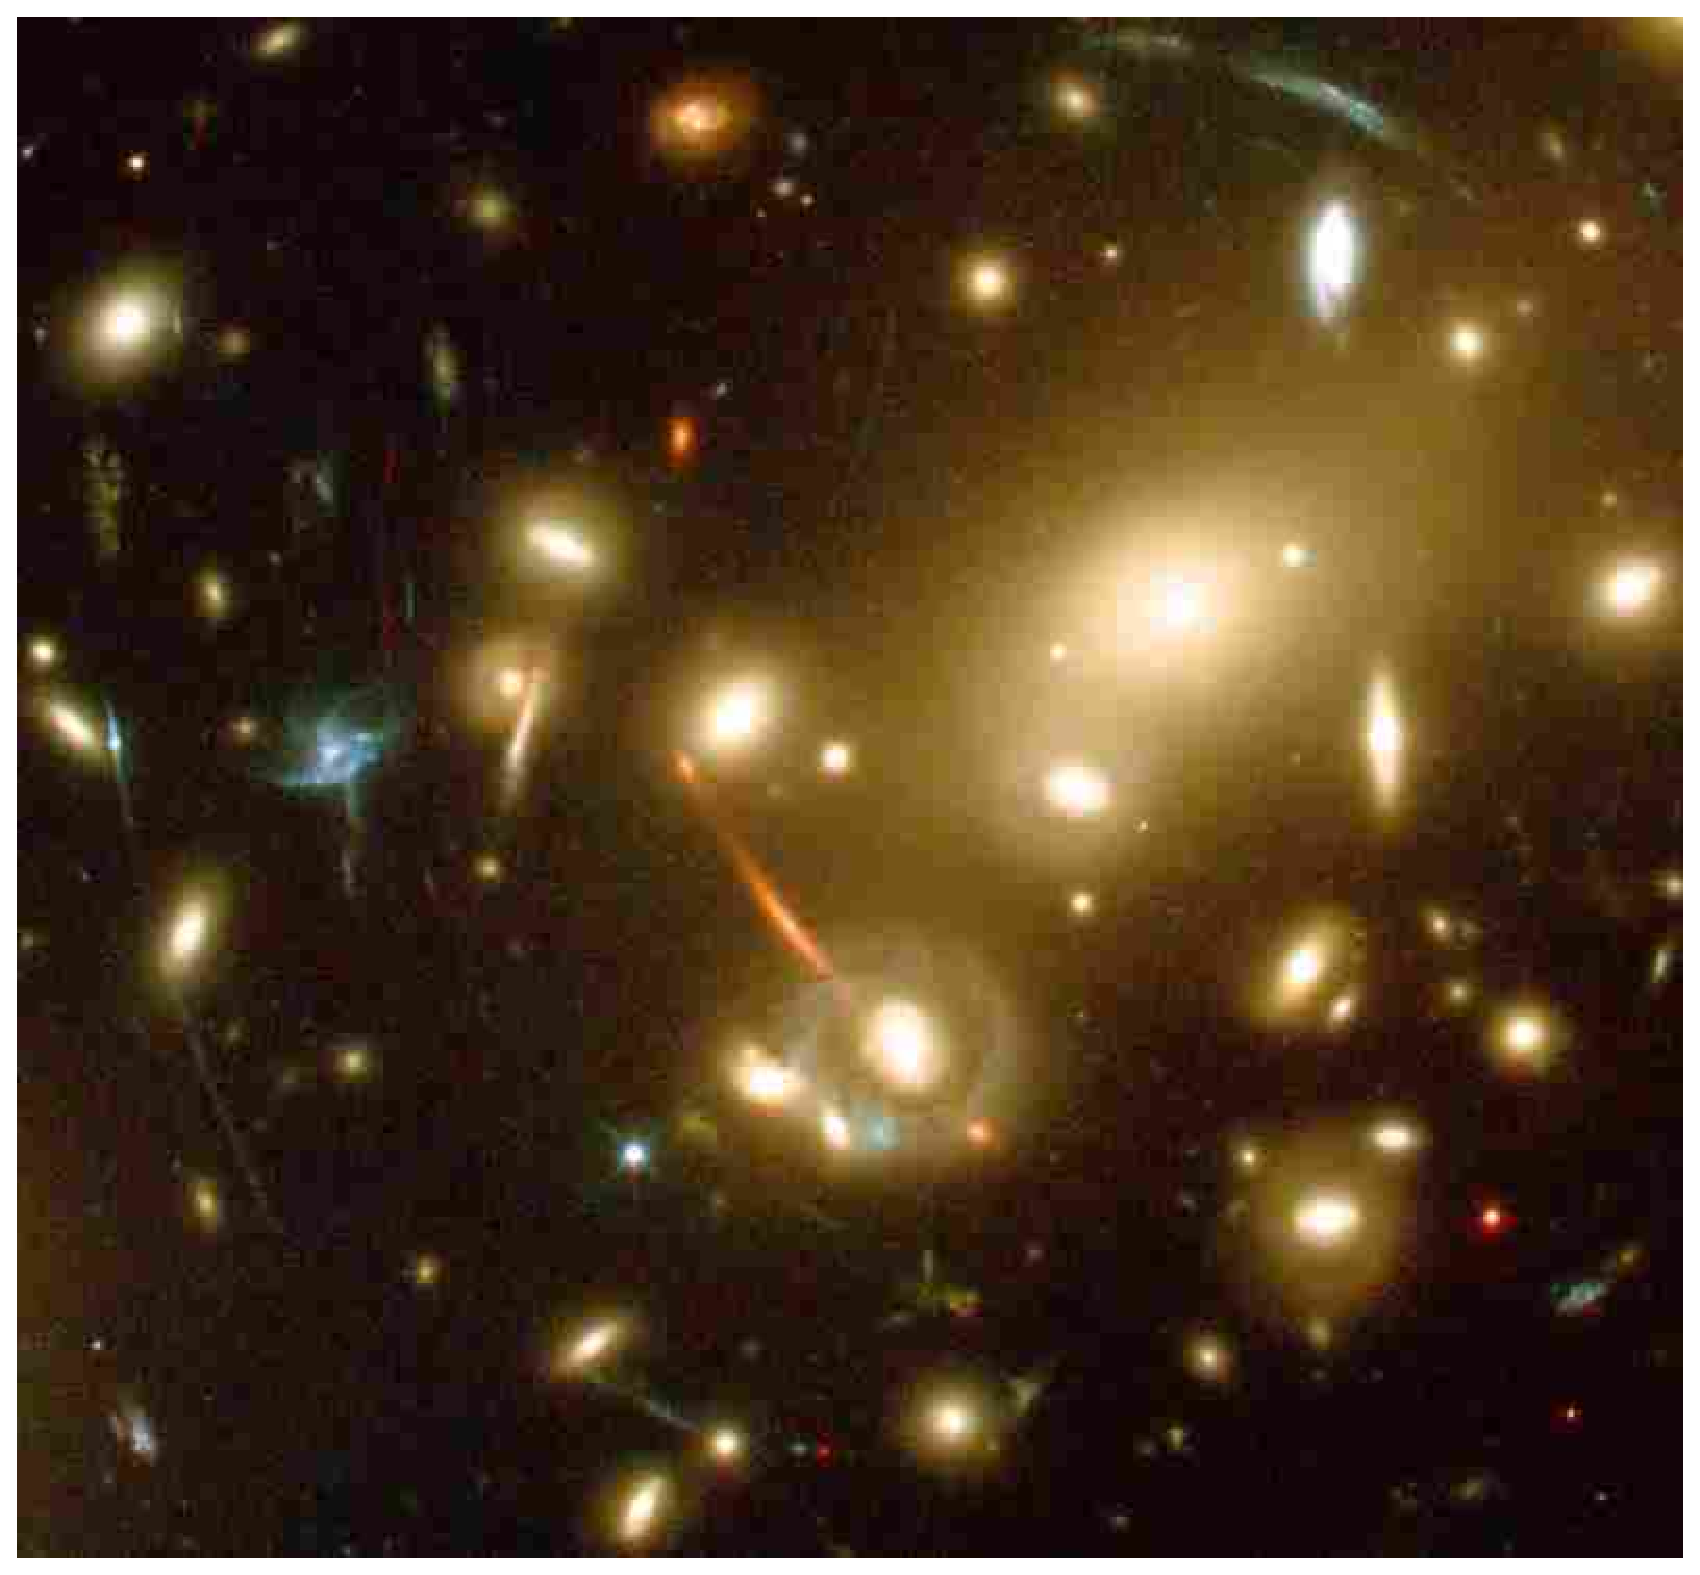
\includegraphics[width=1in]{pictures/gravlens.eps}
}&
\begin{minipage}[b]{1.8in}\textcolor{white}{%
	Heavy objects like dense galaxies and large planets cause light to bend due to gravitational lensing.\vspace{0.2in}}
\end{minipage}
\vspace{0.0in}\\
%
\end{tabular}
}
}}

	\vspace{\VerticalSeparation}

	\psframebox{\parbox[t]{4in}{%Reflection
{
\psset{linestyle=solid}
\textcolor{white}{\Large Reflection}

\begin{itemize}
\item Reflection of EMR is dependent on wavelength as demonstrated when visible light and radio waves bounce off objects that X-Rays would pass through. Microwaves, which have a large wavelength compared to visible light, will bounce off metal mesh in a microwave oven whereas visible light will pass through.
\end{itemize}

\begin{tabular}{cl}
%Mirror
\begin{minipage}[b]{1.8in}\rput(0.97,.3){%Description: reflection schematic
{
\psset{linearc=0}
\psframe[fillstyle=solid,fillcolor=gray,linestyle=solid,linecolor=gray](-.8,.04)(.8,.1)	% Mirror body
\psline[linestyle=dashed,linecolor=gray](0,.1)(0,.7)
\psline[linecolor=gray](-.1,.1)(-.1,.2)(0,.2)
\psline[linecolor=white]{-}(-.8,0.1)(.8,0.1)	%Mirror surface
\rput(0,.1){
	\uput{4pt}[90](-.8;-30){\textcolor{white}{Source}}
	\psline[linecolor=white,fillstyle=none]{->}(-.8;-30)(0,0)(.8;30)
}
\rput(-.2,.5){\textcolor{white}{$\theta_i$}}
\rput(.2,.5){\textcolor{white}{$\theta_r$}}
\psarc[linecolor=white]{<->}(0,.1){.3}{30}{90}
\psarc[linecolor=white]{<->}(0,.1){.3}{90}{150}
\rput[t](0,0){\textcolor{white}{Reflector}}

}
}\end{minipage}&
\hspace{0.0in}\begin{minipage}[b]{1.8in}
	\textcolor{white}{EMR of any wavelength can be reflected, however,
	the reflectivity of a material depends on many factors including
	the wavelength of the incident beam.\vspace{3pt}\\
	The angle of incidence ($\theta_i$) and angle of reflection ($\theta_r$) are the same.}
\end{minipage}\\
\end{tabular}
}



}}

}
}


%If/when copyright permission is ever given for most of these images then this can be restored
%%People

  % People/Discoverers
  %Image specs, mode=greyscale, width=1.00in, dpi=try to retain original up to 1200dpi
  \rput[l]{0}(20.42,17.1){
  	\parbox[t]{1.4in}{
	\scriptsize
	\psset{cornersize=absolute,linearc=4pt,fillstyle=solid,fillcolor=WColor, linecolor=WColor}

	\psframebox{\parbox[t]{1.4in}{\hspace{.18in}
	%\includegraphics{pictures/watt.eps}\\
	
\includegraphics{pictures/unavailable.eps}\\
	\input{pictures/watt.tex}}
	} %1736
	\vspace{0.1in}

	\psframebox{\parbox[t]{1.4in}{\hspace{.18in}
	%\includegraphics{pictures/coulomb.eps}\\
	
\includegraphics{pictures/unavailable.eps}\\
	\input{pictures/coulomb.tex}}
	} %1736
	\vspace{0.1in}

	\psframebox{\parbox[t]{1.4in}{\hspace{.18in}
	%\includegraphics{pictures/volta.eps}\\
	
\includegraphics{pictures/unavailable.eps}\\
	\input{pictures/volta.tex}}
	} %1745
	\vspace{0.1in}

	\psframebox{\parbox[t]{1.4in}{\hspace{.18in}
	%\includegraphics{pictures/ampere.eps}\\
	
\includegraphics{pictures/unavailable.eps}\\
	\input{pictures/ampere.tex}}
	} %1775
	\vspace{0.1in}

	\psframebox{\parbox[t]{1.4in}{\hspace{.18in}
	%\includegraphics{pictures/ohm.eps}\\
	
\includegraphics{pictures/unavailable.eps}\\
	\input{pictures/ohm.tex}}
	} %1789
	\vspace{0.1in}

	\psframebox{\parbox[t]{1.4in}{\hspace{.18in}
	%\includegraphics{pictures/meter.eps}\\
	
\includegraphics{pictures/unavailable.eps}\\
	\input{pictures/meter.tex}}
	} %1791
	\vspace{0.1in}

	\psframebox{\parbox[t]{1.4in}{\hspace{.18in}
	%\includegraphics{pictures/faraday.eps}\\
	
\includegraphics{pictures/unavailable.eps}\\
	\input{pictures/faraday.tex}}
	} %1791
	\vspace{0.1in}

	\psframebox{\parbox[t]{1.4in}{\hspace{.18in}\includegraphics{pictures/siemens.eps}
	\rput[tl]{90}(.05,0){Siemens-AG Siemens-Archiv}\\ \input{pictures/siemens.tex}}} %1816
	\vspace{0.1in}

	\psframebox{\parbox[t]{1.4in}{\hspace{.18in}
	%\includegraphics{pictures/joule.eps}\\
	
\includegraphics{pictures/unavailable.eps}\\
	\input{pictures/joule.tex}}
	} %1818
	\vspace{0.1in}

	\psframebox{\parbox[t]{1.4in}{\hspace{.18in}
	%\includegraphics{pictures/maxwell.eps}\\
	
\includegraphics{pictures/unavailable.eps}\\
	\input{pictures/maxwell.tex}}
	} %1831
	\vspace{0.1in}

	\psframebox{\parbox[t]{1.4in}{\hspace{.18in}
	%\includegraphics{pictures/bell.eps}\\
	
\includegraphics{pictures/unavailable.eps}\\
	\input{pictures/bell.tex}}
	} %1847
	\vspace{0.1in}

	\psframebox{\parbox[t]{1.4in}{\hspace{.18in}
	%\includegraphics{pictures/tesla.eps}\\
	\includegraphics{pictures/unavailable.eps}\\
	\input{pictures/tesla.tex}}
	} %1856
	\vspace{0.1in}

	\psframebox{\parbox[t]{1.4in}{\hspace{.18in}
	%\includegraphics{pictures/hertz.eps}\\
	\includegraphics{pictures/unavailable.eps}\\
	\input{pictures/hertz.tex}}
	} %1857
	\vspace{0.1in}

	\psframebox{\parbox[t]{1.4in}{\hspace{.18in}
	%\includegraphics{pictures/planck.eps}\\
	\includegraphics{pictures/unavailable.eps}\\
	\input{pictures/planck.tex}}
	} %1858

	}
  }


  \rput[B]{0}(15.4,-.6){
\psset{%
	fillcolor=white, 
	fillstyle=solid,
	cornersize=absolute,
	linearc=4pt,
	fillstyle=solid,
	fillcolor=white,
	linestyle=solid,
	linewidth=2pt,
	linecolor=FColor}


%\rput{0}(0,0){\psframebox{\parbox[t]
%	{1in}{\centering \url{unihedron.com}}}}

\rput{0}(0,0){\psframebox{\centering \copyright \hspace{0.1in} \url{unihedron.com}  \hspace{0.2in} \textcolor{gray}{\number\year-\number\month-\number\day}}}

}

\end{pspicture}

\end{document} %===============================================================
